\chapter{Bayes' Theorem and Bayesian Inference}\label{ch:05}

\providecommand{\FiveAMedJointD}{}\renewcommand{\FiveAMedJointD}{0.0095}
\providecommand{\FiveAMedJointH}{}\renewcommand{\FiveAMedJointH}{0.099}
\providecommand{\FiveAMedPpos}{}\renewcommand{\FiveAMedPpos}{0.1085}
\providecommand{\FiveAMedPost}{}\renewcommand{\FiveAMedPost}{0.08756}
\providecommand{\FiveAMontyPE}{}\renewcommand{\FiveAMontyPE}{0.5}
\providecommand{\FiveAMontyPostA}{}\renewcommand{\FiveAMontyPostA}{0.3333}
\providecommand{\FiveAMontyPostB}{}\renewcommand{\FiveAMontyPostB}{0.6667}
\providecommand{\FiveATrigJointS}{}\renewcommand{\FiveATrigJointS}{0.045}
\providecommand{\FiveATrigJointB}{}\renewcommand{\FiveATrigJointB}{0.019}
\providecommand{\FiveATrigPE}{}\renewcommand{\FiveATrigPE}{0.064}
\providecommand{\FiveATrigPost}{}\renewcommand{\FiveATrigPost}{0.7031}
\providecommand{\FiveABallPa}{}\renewcommand{\FiveABallPa}{0.1118}
\providecommand{\FiveABallPb}{}\renewcommand{\FiveABallPb}{0.5578}
\providecommand{\FiveABallPc}{}\renewcommand{\FiveABallPc}{0.311}
\providecommand{\FiveABallPd}{}\renewcommand{\FiveABallPd}{0.01937}
\providecommand{\FiveABallLRbc}{}\renewcommand{\FiveABallLRbc}{1.794}
\providecommand{\FiveAGrbPriorG}{}\renewcommand{\FiveAGrbPriorG}{0.3846}
\providecommand{\FiveAGrbPriorB}{}\renewcommand{\FiveAGrbPriorB}{0.1026}
\providecommand{\FiveAGrbPriorD}{}\renewcommand{\FiveAGrbPriorD}{0.5128}
\providecommand{\FiveAGrbSigOne}{}\renewcommand{\FiveAGrbSigOne}{0.4595}
\providecommand{\FiveAGrbLG}{}\renewcommand{\FiveAGrbLG}{0.004776}
\providecommand{\FiveAGrbLB}{}\renewcommand{\FiveAGrbLB}{0.004006}
\providecommand{\FiveAGrbLD}{}\renewcommand{\FiveAGrbLD}{6.629\times10^{-5}}
\providecommand{\FiveAGrbMaG}{}\renewcommand{\FiveAGrbMaG}{0.8051}
\providecommand{\FiveAGrbMaB}{}\renewcommand{\FiveAGrbMaB}{0.18}
\providecommand{\FiveAGrbMaD}{}\renewcommand{\FiveAGrbMaD}{0.0149}
\providecommand{\FiveAGrbMbG}{}\renewcommand{\FiveAGrbMbG}{0.4088}
\providecommand{\FiveAGrbMbB}{}\renewcommand{\FiveAGrbMbB}{0.04486}
\providecommand{\FiveAGrbMbD}{}\renewcommand{\FiveAGrbMbD}{0.5463}
\providecommand{\FiveAGrbForgotG}{}\renewcommand{\FiveAGrbForgotG}{0.9011}
\providecommand{\FiveAGrbForgotB}{}\renewcommand{\FiveAGrbForgotB}{0.09887}
\providecommand{\FiveAGrbNphot}{}\renewcommand{\FiveAGrbNphot}{68}
\providecommand{\FiveAGrbNtrue}{}\renewcommand{\FiveAGrbNtrue}{25}
\providecommand{\FiveAGrbNest}{}\renewcommand{\FiveAGrbNest}{23.65}
\providecommand{\FiveABdtPostNine}{}\renewcommand{\FiveABdtPostNine}{0.8804}
\providecommand{\FiveABdtPostEight}{}\renewcommand{\FiveABdtPostEight}{0.3926}
\providecommand{\FiveABdtPostNineTiny}{}\renewcommand{\FiveABdtPostNineTiny}{0.06795}
\providecommand{\FiveABdtEffS}{}\renewcommand{\FiveABdtEffS}{0.3446}
\providecommand{\FiveABdtEffB}{}\renewcommand{\FiveABdtEffB}{0.0016}
\providecommand{\FiveABdtCutLR}{}\renewcommand{\FiveABdtCutLR}{215.4}
\providecommand{\FiveABdtCutPur}{}\renewcommand{\FiveABdtCutPur}{0.6851}
\providecommand{\FiveABdtMC}{}\renewcommand{\FiveABdtMC}{0.882}
\providecommand{\FiveABdtMCerr}{}\renewcommand{\FiveABdtMCerr}{0.006818}
\providecommand{\FiveABdtNsel}{}\renewcommand{\FiveABdtNsel}{2238}
\providecommand{\FiveABdtHalfOne}{}\renewcommand{\FiveABdtHalfOne}{0.8223}
\providecommand{\FiveABdtHalfTiny}{}\renewcommand{\FiveABdtHalfTiny}{0.9556}
\providecommand{\FiveACoinHeads}{}\renewcommand{\FiveACoinHeads}{16}
\providecommand{\FiveACoinN}{}\renewcommand{\FiveACoinN}{50}
\providecommand{\FiveACoinMaxDiff}{}\renewcommand{\FiveACoinMaxDiff}{1.041\times10^{-16}}
\providecommand{\FiveACoinPostMean}{}\renewcommand{\FiveACoinPostMean}{0.3269}
\providecommand{\FiveACoinModeFour}{}\renewcommand{\FiveACoinModeFour}{0.4}
\providecommand{\FiveACoinModeForty}{}\renewcommand{\FiveACoinModeForty}{0.268}
\providecommand{\FiveACoinLRh}{}\renewcommand{\FiveACoinLRh}{0.1461}
\providecommand{\FiveACoinLRt}{}\renewcommand{\FiveACoinLRt}{-0.2218}
\providecommand{\FiveACoinKLone}{}\renewcommand{\FiveACoinKLone}{0.03574}
\providecommand{\FiveACoinKLzero}{}\renewcommand{\FiveACoinKLzero}{0.03786}
\providecommand{\FiveACoinTossesHundred}{}\renewcommand{\FiveACoinTossesHundred}{55.97}
\providecommand{\FiveASeqPa}{}\renewcommand{\FiveASeqPa}{0.6154}
\providecommand{\FiveASeqPb}{}\renewcommand{\FiveASeqPb}{0.7191}
\providecommand{\FiveASeqPc}{}\renewcommand{\FiveASeqPc}{0.5059}
\providecommand{\FiveASeqPd}{}\renewcommand{\FiveASeqPd}{0.621}
\providecommand{\FiveASeqArea}{}\renewcommand{\FiveASeqArea}{0.08245}
\providecommand{\FiveAEvFlat}{}\renewcommand{\FiveAEvFlat}{0.08993}
\providecommand{\FiveAEvTri}{}\renewcommand{\FiveAEvTri}{0.0604}
\providecommand{\FiveAEvFair}{}\renewcommand{\FiveAEvFair}{0.009766}
\providecommand{\FiveAEvSumFlat}{}\renewcommand{\FiveAEvSumFlat}{1}
\providecommand{\FiveAEvSumTri}{}\renewcommand{\FiveAEvSumTri}{1}
\providecommand{\FiveAEvRatio}{}\renewcommand{\FiveAEvRatio}{9.208}
\providecommand{\FiveAScrLRMp}{}\renewcommand{\FiveAScrLRMp}{8.70}
\providecommand{\FiveAScrLRMm}{}\renewcommand{\FiveAScrLRMm}{0.144}
\providecommand{\FiveAScrLRUp}{}\renewcommand{\FiveAScrLRUp}{8.00}
\providecommand{\FiveAScrLRUm}{}\renewcommand{\FiveAScrLRUm}{0.222}
\providecommand{\FiveAScrLRBp}{}\renewcommand{\FiveAScrLRBp}{95.0}
\providecommand{\FiveAScrLRBm}{}\renewcommand{\FiveAScrLRBm}{0.0505}
\providecommand{\FiveAScrP}{}\renewcommand{\FiveAScrP}{0.0808}
\providecommand{\FiveAScrPP}{}\renewcommand{\FiveAScrPP}{0.413}
\providecommand{\FiveAScrPM}{}\renewcommand{\FiveAScrPM}{0.0192}
\providecommand{\FiveAScrPPP}{}\renewcommand{\FiveAScrPPP}{0.9852}
\providecommand{\FiveAScrPPM}{}\renewcommand{\FiveAScrPPM}{0.0343}
\providecommand{\FiveAScrPMP}{}\renewcommand{\FiveAScrPMP}{0.650}
\providecommand{\FiveAScrM}{}\renewcommand{\FiveAScrM}{0.00146}
\providecommand{\FiveAScrMCP}{}\renewcommand{\FiveAScrMCP}{0.0805}
\providecommand{\FiveAScrMCPP}{}\renewcommand{\FiveAScrMCPP}{0.413}
\providecommand{\FiveAScrMCPM}{}\renewcommand{\FiveAScrMCPM}{0.0189}
\providecommand{\FiveAScrMCPPP}{}\renewcommand{\FiveAScrMCPPP}{0.9847}
\providecommand{\FiveAScrCorrHH}{}\renewcommand{\FiveAScrCorrHH}{0.0526}
\providecommand{\FiveAScrCorrLR}{}\renewcommand{\FiveAScrCorrLR}{13.2}
\providecommand{\FiveAScrCorrPost}{}\renewcommand{\FiveAScrCorrPost}{0.118}
\providecommand{\FiveAScrCorrMC}{}\renewcommand{\FiveAScrCorrMC}{0.119}
\providecommand{\FiveAPrbLAp}{}\renewcommand{\FiveAPrbLAp}{11.25}
\providecommand{\FiveAPrbLBp}{}\renewcommand{\FiveAPrbLBp}{17.0}
\providecommand{\FiveAPrbLBm}{}\renewcommand{\FiveAPrbLBm}{0.1579}
\providecommand{\FiveAPrbOzero}{}\renewcommand{\FiveAPrbOzero}{0.005025}
\providecommand{\FiveAPrbA}{}\renewcommand{\FiveAPrbA}{0.0535}
\providecommand{\FiveAPrbAB}{}\renewcommand{\FiveAPrbAB}{0.490}
\providecommand{\FiveAPrbAb}{}\renewcommand{\FiveAPrbAb}{0.00885}
\providecommand{\FiveAPrbOAB}{}\renewcommand{\FiveAPrbOAB}{0.9611}
\providecommand{\FiveAPrbOAb}{}\renewcommand{\FiveAPrbOAb}{0.008926}
\providecommand{\FiveAPrbN}{}\renewcommand{\FiveAPrbN}{4}
\providecommand{\FiveAPrbNminus}{}\renewcommand{\FiveAPrbNminus}{0.877}
\providecommand{\FiveAPrbNpost}{}\renewcommand{\FiveAPrbNpost}{0.9877}
\providecommand{\FiveAPrbqA}{}\renewcommand{\FiveAPrbqA}{0.05155}
\providecommand{\FiveAPrbqB}{}\renewcommand{\FiveAPrbqB}{0.02062}
\providecommand{\FiveAPrbHAB}{}\renewcommand{\FiveAPrbHAB}{0.03103}
\providecommand{\FiveAPrbHAb}{}\renewcommand{\FiveAPrbHAb}{0.04897}
\providecommand{\FiveAPrbABc}{}\renewcommand{\FiveAPrbABc}{0.110}
\providecommand{\FiveAPrbAbc}{}\renewcommand{\FiveAPrbAbc}{0.0137}
\providecommand{\FiveAPrbLRABc}{}\renewcommand{\FiveAPrbLRABc}{24.7}
\providecommand{\FiveAPrbLRABi}{}\renewcommand{\FiveAPrbLRABi}{191}
\providecommand{\FiveAPrbMCAB}{}\renewcommand{\FiveAPrbMCAB}{0.489}
\providecommand{\FiveAPrbMCAb}{}\renewcommand{\FiveAPrbMCAb}{0.00898}
\providecommand{\FiveAPrbMCABc}{}\renewcommand{\FiveAPrbMCABc}{0.110}
\providecommand{\FiveAPrbMCAbc}{}\renewcommand{\FiveAPrbMCAbc}{0.0139}
 
\section*{Where this chapter is going}
\label{5a:sec:roadmap}

Nature produced one set of data. Several situations could have produced it: a
disease or no disease, signal or background, a fair coin or a biased one, a
universe with one value of $\Omega_m$ or another. Physics usually tells us how
each situation \emph{generates} data. What we want is the reverse: given the
data we actually have, how should probability be spread over the situations that
could have produced them? Bayes' theorem is the rule that turns the first kind
of knowledge into the second, and one picture carries it throughout. Before the
evidence, the whole sample space is in play. The evidence tells us that we are
somewhere in the region where it is true, so the sample space shrinks to that
region, and every hypothesis is re-measured by the share of the surviving region
it occupies.

With a handful of discrete hypotheses the picture can be drawn and computed by
hand. Credibility is reallocated: hypotheses that predicted the observation well
gain, the others lose, and the total stays one. The ratio of two hypotheses
changes by a single factor, the likelihood ratio, so evidence multiplies odds and
adds in logarithms. Observations arriving one by one are absorbed one by one, the
posterior of each step becoming the prior of the next, and the order does not
matter. The denominator of the theorem is the sum over every path that could have
led to the observation. When the hypotheses become the values of a continuous
parameter, the list becomes a density, the likelihood comes from a model of the
noise, and we need ways to summarise a posterior and to integrate out parameters
we do not care about. Finally the hypotheses can be whole models with their own
parameters. Then the denominator, the evidence, is what compares them, and
computing it in many dimensions is so hard that it motivates the sampling methods
of \cref{ch:09}.

Bayes' theorem is the last arrow of the pipeline of \cref{0a:sec:pipeline}: it
takes the sampling distribution $P(S\given\theta)$ of a summary $S$ and turns it
into a statement about the physics. \Cref{ch:02,ch:03,ch:04} built the forward object $P(S\given\theta)$; here
it is read backwards.

\begin{figure}[htbp]
\centering
\begin{tikzpicture}[
  node distance=6mm and 5mm,
  blk/.style={draw=accent,thick,rounded corners=2pt,fill=ideabg,
              align=center,font=\small,minimum height=10mm,text width=27mm},
  hot/.style={blk,fill=defbg,draw=fibreorange!80!black},
  flow/.style={->,thick,accent}]
  \node[blk] (fwd) {forward model\\ $\Prob(E\given H_i)$\\ \footnotesize(\cref{ch:02,ch:03,ch:04})};
  \node[hot,right=of fwd] (shrink) {evidence shrinks\\ the sample\\ space:\\ $\Prob(H_i\given E)$};
  \node[hot,right=of shrink] (odds) {odds $\times$\\ likelihood ratio;\\ sequential updates};
  \node[hot,right=of odds] (den) {denominator $=$\\ sum over all paths};
  \node[hot,below=10mm of den] (cont) {continuous $\theta$:\\ $p(\theta\given\data)$, priors,\\ marginalisation};
  \node[hot,left=of cont] (model) {models $M_i$:\\ evidence $Z$,\\ Bayes factors};
  \node[blk,left=of model] (mcmc) {why we sample:\\ MCMC \footnotesize(\cref{ch:09})};
  \node[blk,left=of mcmc] (fish) {curvature of\\ the log posterior:\\ Fisher \footnotesize(\cref{ch:10})};
  \draw[flow] (fwd) -- (shrink);
  \draw[flow] (shrink) -- (odds);
  \draw[flow] (odds) -- (den);
  \draw[flow] (den) -- (cont);
  \draw[flow] (cont) -- (model);
  \draw[flow] (model) -- (mcmc);
  \draw[flow] (cont.south) to[out=-150,in=-30] (fish.south);
\end{tikzpicture}
\caption{How the ideas of Bayesian inference connect. The top row works with a
list of discrete hypotheses: a forward model gives the probability of the
observation under each, the observation shrinks the sample space, odds change by
the likelihood ratio, and the denominator collects every path to the
observation. The bottom row replaces the list by a continuous parameter and then
by competing models; the cost of the denominator in many dimensions leads to
Markov chain Monte Carlo, and the curvature of the log posterior near its peak
leads to the Fisher matrix. The boxes with blue borders belong to other chapters.}
\label{5a:fig:roadmap}
\end{figure}

\section{One joint table, read in two directions}
\label{5a:sec:two-directions}

A collider experiment writes an event to disk because its first-level trigger
fired. Three independent trigger paths can fire it: the muon system, the
calorimeter, and a fast track trigger. From the trigger rates we know what share
of the recorded events each path is responsible for: $25\%$ muon, $60\%$
calorimeter, $15\%$ track. The event record of one particular event has lost the
flag that says which path fired. Offline, the reconstruction finds an isolated
muon with large transverse momentum in it. Which path most probably fired the
trigger?

The physics of each trigger tells us something in the \emph{forward} direction. If
the muon path fired, the event contains an isolated high-$p_T$ muon $70\%$ of the
time (the rest are fakes and muons outside the offline acceptance). If the
calorimeter path fired, only $5\%$ of such events contain one. If the track path
fired, $20\%$ do. These numbers answer ``given the path, what do we see?''. We
want the reverse: ``given what we see, which path?''.

The two questions use probability in two opposite directions. In the first, we
fix one possible situation (here, the path that fired) and ask what it can lead
to: which outcomes, and how probable each one is. The outcome is still
uncertain, and probability forecasts it. This is \newterm{prediction}. In the
second, the outcome has already happened: the muon is on disk. Several
situations could have led to it, and we want to know which one did. So we start
from the outcome and work back to its possible sources. We ask which hypotheses
could have produced what we saw, and how probable each one is now that we have
seen it. This is \newterm{inference}. We met the two directions in \cref{ch:00}
and read a first tree backwards in \cref{ch:01}. All of Bayesian inference rests
on this one step: turning the forward question into the backward one.

\paragraph{The question in words.}
Every backward question can be put into four short questions before a single
symbol is written:
\begin{enumerate}[itemsep=1pt]
  \item What did we actually see?
  \item Which hypotheses could have given rise to it?
  \item Under each of those hypotheses, how probable was what we saw?
  \item In the light of that evidence, how must the probabilities we gave the
        hypotheses beforehand be revised?
\end{enumerate}
For the trigger: (1) we observed an isolated high-$p_T$ muon, call it $E$;
(2) the three paths $H_\mu$, $H_{\rm cal}$, $H_{\rm trk}$ could have produced
it, and exactly one of them fired this event (we ignore the rare events fired
by two paths at once); (3) the observation had probability $0.70$, $0.05$ and
$0.20$ under them; (4) the original probabilities $0.25$, $0.60$, $0.15$ must
be updated in the light of $E$.
Steps 1 to 3 are prediction, done once for each hypothesis. Only step 4 is new.

\subsection{Deduction runs forward, inference runs backward}

The same two directions appear in the difference between deduction and
inference \srcref{Sivia}{\S1.1, Fig.~1.1}. In \emph{deductive} reasoning the
cause is given and we work out its consequences. If a coin is fair, the
probability of seven heads in ten tosses follows by counting. Pure mathematics,
and every game of chance, runs this way. Most of science runs the other way. We
see the effects and ask for the cause: ten tosses gave seven heads; is the coin
fair? Several causes could have produced the same effect, so no amount of logic
makes the answer certain. Sivia calls this \emph{plausible reasoning}. The
question is whether plausible reasoning has rules we can compute with.

It does, and they are the rules of probability we already know. Cox asked a
plain question: if we give numbers to degrees of belief, what rules must those
numbers obey for the reasoning to be consistent? Consistent means, among other
things, that two different ways of using the same information must give the same
answer. His answer was that any such numbers can be relabelled so that they obey
exactly two rules \srcref{Sivia}{\S1.2, (1.1)--(1.2)}:
\begin{align}
  \Prob(X\given I)+\Prob(\bar X\given I)&=1
  &&\text{(sum rule)},\label{5a:eq:sum}\\
  \Prob(X,Y\given I)&=\Prob(X\given Y,I)\,\Prob(Y\given I)
  &&\text{(product rule)}.\label{5a:eq:product}
\end{align}
Here $\bar X$ \unpack{``$X$ is false''} is the complement, the comma means
``and'', and $I$ is the \newterm{background information}
\unpack{everything we take as given, such as the trigger rates and the detector
model}. Every probability in inference is conditional on some $I$, even when we
stop writing it. Many heated arguments about data analysis are really arguments
about an $I$ that nobody wrote down \srcref{Sivia}{\S1.2}.

The product rule already contains Bayes' theorem. The joint statement ``$X$ and
$Y$'' is the same statement as ``$Y$ and $X$'', so the product rule can be applied
in either order and must give the same number:
\begin{align}
  \Prob(X\given Y,I)\,\Prob(Y\given I)
  &\eqby{1}\Prob(X,Y\given I)
  \eqby{2}\Prob(Y,X\given I)
  \eqby{3}\Prob(Y\given X,I)\,\Prob(X\given I).\nonumber
\intertext{Dividing by $\Prob(Y\given I)>0$,}
  \Prob(X\given Y,I)
  &\eqby{4}\frac{\Prob(Y\given X,I)\,\Prob(X\given I)}{\Prob(Y\given I)} .
  \label{5a:eq:bayes-xy}
\end{align}
\begin{explain}
  \item Product rule \eqref{5a:eq:product}.
  \item ``$X$ and $Y$'' is logically the same proposition as ``$Y$ and $X$''.
  \item Product rule again, with the roles of $X$ and $Y$ exchanged.
  \item Divide both sides of the first line by $\Prob(Y\given I)$.
\end{explain}
Put $X=H$, a hypothesis, and $Y=E$, the observed evidence. The theorem turns the
quantity physics hands us, $\Prob(E\given H,I)$, into the quantity we want,
$\Prob(H\given E,I)$ \srcref{Sivia}{\S1.3}, \srcref{Kruschke}{\S5.1.1},
\srcref{Lambert}{\S3.6}.

Bayes' theorem is the first consequence of the two rules. The second is
\newterm{marginalisation} \srcref{Sivia}{(1.5)--(1.7)}: it answers ``how
probable is $E$ when we do not know which hypothesis is true?''. If $H_1,\dots,H_k$ are \newterm{mutually exclusive
and exhaustive} \unpack{exactly one of them is true}, then
\begin{align}
  \Prob(E\given I)
  &\eqby{1}\sum_{i=1}^k\Prob(E,H_i\given I)
  \eqby{2}\sum_{i=1}^k\Prob(E\given H_i,I)\,\Prob(H_i\given I) .
  \label{5a:eq:marg}
\end{align}
\begin{explain}
  \item $E$ happens together with exactly one of the $H_i$, so its probability
        is the sum of the probabilities of the $k$ disjoint pieces $E\cap H_i$.
        This is the law of total probability of \cref{ch:01}; Sivia derives it
        from the sum and product rules alone.
  \item Product rule on each term.
\end{explain}
It is the denominator of Bayes' theorem, and it will get a section of its own
(\cref{5a:sec:denominator}).

Put $X=H_i$ in \eqref{5a:eq:bayes-xy} and replace the denominator by the
marginalisation \eqref{5a:eq:marg}. For mutually exclusive and exhaustive hypotheses
$H_1,\dots,H_k$ and an observation $E$ with $\Prob(E)>0$ this gives the working form
of Bayes' theorem:
\begin{equation}
  \underbrace{\Prob(H_i\given E)}_{\text{posterior}}
  =\frac{\overbrace{\Prob(E\given H_i)}^{\text{likelihood}}\;
         \overbrace{\Prob(H_i)}^{\text{prior}}}
        {\underbrace{\textstyle\sum_{j}\Prob(E\given H_j)\,\Prob(H_j)}_{\text{evidence }\Prob(E)}} .
  \label{5a:eq:bayes}
\end{equation}

\begin{keyidea}[Bayes' theorem in words]
Posterior $=$ likelihood $\times$ prior $/$ evidence. It is the product rule applied in
both orders. The numerator is one path through the tree; the denominator is the sum
over every path that ends in $E$.
\end{keyidea}

\subsection{The tree and the trigger}

Draw the trigger problem as a tree (\cref{5a:fig:trigger-tree}). The first split
is nature's choice of path, with the priors on the branches. The second split is
what the offline reconstruction sees, with the forward probabilities on the
branches. Multiplying along a path gives the probability of the leaf, the joint
probability $\Prob(H_i\cap E)$.

\begin{figure}[htbp]
\centering
\begin{tikzpicture}[
  font=\small,
  lvl/.style={draw=accent,rounded corners=2pt,fill=ideabg,minimum width=14mm,
              minimum height=6mm,align=center},
  leafE/.style={draw=formblue,thick,fill=formblue!12,rounded corners=2pt,
                minimum width=12mm,minimum height=6mm},
  leafN/.style={draw=softgray,rounded corners=2pt,minimum width=12mm,
                minimum height=6mm,text=softgray}]
  \node[lvl] (root) at (0,0) {event};
  \node[lvl] (mu)  at (-4.2,-1.8) {$H_\mu$};
  \node[lvl] (cal) at ( 0.0,-1.8) {$H_{\rm cal}$};
  \node[lvl] (trk) at ( 4.2,-1.8) {$H_{\rm trk}$};
  \draw (root) -- (mu) node[pos=0.5,anchor=south east,xshift=1pt] {$0.25$};
  \draw (root) -- (cal) node[pos=0.5,right=2pt] {$0.60$};
  \draw (root) -- (trk) node[pos=0.5,anchor=south west,xshift=-1pt] {$0.15$};
  \foreach \h/\x/\pe/\pn/\j in {mu/-4.2/0.70/0.30/0.175, cal/0.0/0.05/0.95/0.030, trk/4.2/0.20/0.80/0.030}{
    \node[leafE] (\h E) at (\x-0.9,-3.7) {$E$};
    \node[leafN] (\h N) at (\x+0.9,-3.7) {$\bar E$};
    \draw (\h) -- (\h E) node[pos=0.45,left=2pt] {$\pe$};
    \draw[softgray] (\h) -- (\h N) node[pos=0.45,right=2pt] {$\pn$};
    \node[font=\footnotesize,formblue!70!black] at (\x-0.9,-4.35) {$\j$};
  }
  \node[anchor=west,font=\footnotesize,align=left] at (-6.4,-5.0)
    {leaf probabilities of the observed branch $E$ (products along each path)};
\end{tikzpicture}
\caption{The trigger problem as a tree. Nature first chooses the path that fires,
with the priors on the upper branches; the lower branches give the probability
that each path's events contain an isolated high-$p_T$ muon ($E$) or not
($\bar E$). The observed branch is outlined in blue, and the number under each
blue leaf is the product along its path. Inference keeps only the blue leaves
and asks what share of their total each one carries.}
\label{5a:fig:trigger-tree}
\end{figure}

Prediction reads the tree top-down: pick a path, follow it, get the probability of
each outcome. Inference starts at the bottom. We saw the muon, so we know we are
on a blue leaf, but not on which one. So we collect the three blue leaves and ask
what share of their total each one holds:
\begin{align*}
  \Prob(E)
  &\eqby{1}0.25\times0.70+0.60\times0.05+0.15\times0.20
   =0.175+0.030+0.030=0.235,\\
  \Prob(H_\mu\given E)
  &\eqby{2}\frac{0.175}{0.235}\approx0.745,\qquad
  \Prob(H_{\rm cal}\given E)=\Prob(H_{\rm trk}\given E)=\frac{0.030}{0.235}\approx0.128 .
\end{align*}
\begin{explain}
  \item Marginalisation \eqref{5a:eq:marg}: the sum of the three blue leaves.
  \item Bayes' theorem \eqref{5a:eq:bayes}: one blue leaf over all of them.
\end{explain}
The muon path most probably fired the trigger. The calorimeter path was the most
probable before we looked ($0.60$), and it is now one of the two least probable.
It lost because it rarely produces what we saw. The track path was the least
probable before, and it ends level with the calorimeter path. Only the product of
prior and likelihood enters, so a small prior times a larger likelihood
($0.15\times0.20$) can match a large prior times a small likelihood
($0.60\times0.05$). The prior still matters: the posteriors are \emph{not} the
likelihoods rescaled to sum to one. Those would be $0.70$, $0.05$, $0.20$ divided
by their sum $0.95$, that is $0.74$, $0.05$, $0.21$.

\subsection{The joint table: a column for prediction, a row for inference}

A tree is one way to store a joint distribution. A table is another, and it makes
the two directions of reading especially plain \srcref{Kruschke}{\S5.1.2,
Tables~5.1 and~5.5}. Let the columns be the hypotheses and the rows be the
possible observations. Each cell holds the joint probability
$\Prob(E_r,H_c)=\Prob(E_r\given H_c)\Prob(H_c)$. Summing a column gives the
prior $\Prob(H_c)$ in the bottom margin; summing a row gives $\Prob(E_r)$ in the
right margin. \Cref{5a:fig:joint-table} shows it for the trigger.

\begin{figure}[htbp]
\centering
\begin{tikzpicture}[font=\small]
  \def\cw{2.1}\def\rh{0.75}
  \fill[formblue!16] (0,-\rh) rectangle (4*\cw,0);
  \fill[fibreorange!30,opacity=0.6] (0,-2*\rh) rectangle (\cw,0);
  \draw[fibreorange!80!black,thick] (0,-2*\rh) rectangle (\cw,0);
  \draw[formblue,thick] (0,-\rh) rectangle (4*\cw,0);
  \foreach \i in {0,...,4} \draw[softgray] (\i*\cw,\rh) -- (\i*\cw,-3*\rh);
  \foreach \j in {1,0,-1,-2,-3} \draw[softgray] (-1.4,\j*\rh) -- (4*\cw,\j*\rh);
  \draw[thick] (3*\cw,\rh) -- (3*\cw,-3*\rh);
  \draw[thick] (-1.4,-2*\rh) -- (4*\cw,-2*\rh);
  \node at (0.5*\cw,0.5*\rh) {$H_\mu$};
  \node at (1.5*\cw,0.5*\rh) {$H_{\rm cal}$};
  \node at (2.5*\cw,0.5*\rh) {$H_{\rm trk}$};
  \node at (3.5*\cw,0.5*\rh) {row sum};
  \node[anchor=east] at (-0.1,-0.5*\rh) {$E$};
  \node[anchor=east] at (-0.1,-1.5*\rh) {$\bar E$};
  \node[anchor=east] at (-0.1,-2.5*\rh) {column sum};
  \node at (0.5*\cw,-0.5*\rh) {$0.175$};
  \node at (1.5*\cw,-0.5*\rh) {$0.030$};
  \node at (2.5*\cw,-0.5*\rh) {$0.030$};
  \node at (3.5*\cw,-0.5*\rh) {$0.235$};
  \node at (0.5*\cw,-1.5*\rh) {$0.075$};
  \node at (1.5*\cw,-1.5*\rh) {$0.570$};
  \node at (2.5*\cw,-1.5*\rh) {$0.120$};
  \node at (3.5*\cw,-1.5*\rh) {$0.765$};
  \node at (0.5*\cw,-2.5*\rh) {$0.25$};
  \node at (1.5*\cw,-2.5*\rh) {$0.60$};
  \node at (2.5*\cw,-2.5*\rh) {$0.15$};
  \node at (3.5*\cw,-2.5*\rh) {$1$};
  \fill[fibreorange!18,draw=fibreorange!80!black,thick] (0,-3.9*\rh) rectangle (0.4,-3.5*\rh);
  \node[anchor=west] at (0.5,-3.7*\rh) {prediction: one column, divided by its sum};
  \fill[formblue!16,draw=formblue,thick] (0,-4.7*\rh) rectangle (0.4,-4.3*\rh);
  \node[anchor=west] at (0.5,-4.5*\rh) {inference: the observed row, divided by its sum};
\end{tikzpicture}
\caption{The joint probabilities of trigger path (columns) and offline
observation (rows). A prediction fixes a hypothesis and looks down its column:
$0.175/0.25=0.70$ is the probability of seeing the muon if the muon path fired.
An inference fixes the observation and looks along its row: $0.175/0.235=0.745$
is the probability that the muon path fired given that we see the muon. Both
divide the same cell, by different sums.}
\label{5a:fig:joint-table}
\end{figure}

Now the two directions are two ways of dividing the same cell. Prediction fixes a
column and divides by the column sum: $\Prob(E\given H_\mu)=0.175/0.25$.
Inference fixes the row we observed and divides by the row sum:
$\Prob(H_\mu\given E)=0.175/0.235$. Observing $E$ means \emph{restricting
attention to one row of the table} \srcref{Kruschke}{\S5.2}. The other row, $\bar
E$, is still a perfectly good row. It is simply not what happened, and it drops out
of every calculation. That is the shrinking of the sample space in its most
compact form. \Cref{5a:sec:shrink} draws it to scale.

The table also shows why the forward numbers are called a
\newterm{likelihood} rather than a probability once we read them the inference
way \srcref{Lambert}{\S4.4}. Along a column, the forward probabilities of all
possible observations sum to one: $0.70+0.30=1$. Along the observed row, the
forward probabilities $\Prob(E\given H_c)$ of that \emph{one} observation under the
different hypotheses are $0.70$, $0.05$, $0.20$. They sum to $0.95$, and nothing
forces them to sum to one. Read along a row they are a function of the
hypothesis, not a distribution over it.

\paragraph{Example: a coin table.}
Lambert makes the same point with a coin allowed only six values of its
probability of heads, $\theta\in\{0,0.2,0.4,0.6,0.8,1\}$, tossed twice
\srcref{Lambert}{\S4.4, Table~4.1}. The number of heads $X$ is binomial, so the
table entries are $\Prob(X\given\theta)=\binom{2}{X}\theta^X(1-\theta)^{2-X}$:
\begin{center}
\small
\begin{tabular}{@{}c|ccc|c@{}}
\toprule
$\theta$ & $X=0$ & $X=1$ & $X=2$ & sum over $X$\\
\midrule
0.0 & 1.00 & 0.00 & 0.00 & 1\\
0.2 & 0.64 & 0.32 & 0.04 & 1\\
0.4 & 0.36 & 0.48 & 0.16 & 1\\
0.6 & 0.16 & 0.48 & 0.36 & 1\\
0.8 & 0.04 & 0.32 & 0.64 & 1\\
1.0 & 0.00 & 0.00 & 1.00 & 1\\
\midrule
sum over $\theta$ & 2.20 & 1.60 & 2.20 & \\
\bottomrule
\end{tabular}
\end{center}
Each row (fixed $\theta$) is a probability distribution for the data: it sums to
one. Each column (fixed data) is a likelihood: for $X=1$ it sums to $1.60$. The
same happens for a continuous $\theta\in[0,1]$. With one head in two tosses,
\begin{align*}
  \int_0^1\Prob(X=1\given\theta)\,\dd\theta
  \eqby{1}\int_0^1 2\theta(1-\theta)\,\dd\theta
  \eqby{2}2\Bigl(\frac12-\frac13\Bigr)=\frac13\neq1 .
\end{align*}
\begin{explain}
  \item The binomial probability of one head in two tosses.
  \item $\int_0^1\theta\,\dd\theta=\frac12$ and $\int_0^1\theta^2\,\dd\theta=\frac13$.
\end{explain}
A likelihood has no reason to integrate to one over the parameter. That is why
Bayes' theorem needs both a prior, to turn it into a joint probability, and a
denominator, to normalise the row.

\begin{pitfall}[A likelihood is not a probability of the hypothesis]
$\Prob(E\given H)$ read as a function of $H$ is a likelihood. It can be large for
two hypotheses at once, and its sum over hypotheses means nothing. ``The muon
path explains the data with probability $0.70$'' is a misreading: $0.70$ is the
probability of the data if the muon path fired. The probability of the path is
$0.745$ here, and only because of the particular priors.
\end{pitfall}

\subsection{Logical, not causal, connections}

Inference runs backwards in logic, not in time. A later event cannot cause an
earlier one, but it can still tell us about it. Jaynes' example shows this
\srcref{Sivia}{\S1.4}.

\paragraph{Example: the second ball tells us about the first.}
A bag holds five red and seven green balls. We draw two, one after the other,
without putting the first back.

\emph{The event.} We are not told the colour of the first ball. We are told that
the second is green. Call this $G_2$.

\emph{The question.} Is the probability that the first ball was red still
$5/12$, as it was before we heard about the second? The first draw happened
before the second, so the second cannot have caused it. But the second can be
evidence about it.

\emph{The candidates.} There are two: the first ball was red ($R_1$) or green
($G_1$). Under each, the second draw is a draw from a different bag. After a red
first ball the bag holds $4$ red and $7$ green, so a green second ball has
probability $7/11$. After a green first ball it holds $5$ red and $6$ green, so a
green second ball has probability $6/11$. A green second ball is a little more
likely if the first was red, because the first draw then left all seven greens
in the bag.

\emph{Only then the numbers.} The priors are $\Prob(R_1)=5/12$ and
$\Prob(G_1)=7/12$:
\begin{align*}
  \Prob(G_2)
  &\eqby{1}\Prob(G_2\given R_1)\Prob(R_1)+\Prob(G_2\given G_1)\Prob(G_1)
   =\frac{7}{11}\cdot\frac{5}{12}+\frac{6}{11}\cdot\frac{7}{12}
   =\frac{35+42}{132}=\frac{7}{12},\\
  \Prob(R_1\given G_2)
  &\eqby{2}\frac{\Prob(G_2\given R_1)\Prob(R_1)}{\Prob(G_2)}
   =\frac{35/132}{77/132}=\frac{5}{11} .
\end{align*}
\begin{explain}
  \item Marginalisation over the first draw, with $\Prob(G_2\given R_1)=7/11$ and
        $\Prob(G_2\given G_1)=6/11$ found above.
  \item Bayes' theorem.
\end{explain}
The answer moved from $5/12\approx0.417$ to $5/11\approx0.455$. The extreme case
makes it obvious: with one red and one green ball in the bag, a green second ball
means the first was red with certainty. A conditional probability records what
one statement \emph{tells us} about another, not what causes what. Inference from
the leaves of a tree back to its first split works the same way: the observation
comes later in the physics, but it tells us about what happened first.

\subsection{What the probabilities mean}

There are two readings of what a probability is, and Wasserman sets them side by
side \mainref{pp.~175--176}. The frequentist reading rests on three postulates.
Probability is a long-run relative frequency. Parameters are fixed constants, so
no probability statements are made about them. A procedure is judged by how
often it gives the right answer over many repetitions. The Bayesian reading rests
on three others. Probability describes a degree of belief. We may therefore make
probability statements about parameters. Inference about a parameter means
producing a probability distribution for it. The second reading is the one that
lets us give a probability to a one-off event. The weather forecast's ``$90\%$
chance of rain tomorrow'' is such a probability \srcref{SeeingTheory}{p.~49}. So is
Laplace's posterior for the mass of Saturn. He summarised it as a bet of
$11\,000$ to $1$ that his estimate was not wrong by more than $1\%$. A further
$150$ years of data changed the estimate by only $0.63\%$ \srcref{Sivia}{\S1.4}.

For the trigger path both readings work. Which path fires is the outcome of a
process that repeats with every event, and $0.745$ is the fraction of recorded
events with an isolated muon that were fired by the muon path. A physical
constant is different: nature chose its value once, so only the degree-of-belief
reading is available. The arithmetic of \eqref{5a:eq:bayes} is the same either
way. A degree of belief is not arbitrary: two people with the same background
information $I$ must assign the same probabilities \srcref{Sivia}{\S1.4}. When
they disagree, they disagree about $I$, and Bayes' theorem forces each of them
to write $I$ down.
\section{Information shrinks the sample space}
\label{5a:sec:shrink}

A disease affects one person in a hundred. A test for it comes out positive for
$95\%$ of the people who have the disease and, falsely, for $10\%$ of the people
who do not. A person picked at random tests positive. How worried should they
be? Most people's first answer is ``about $95\%$''. The right answer is about
$9\%$. We computed it by formula in
\cref{ch:01}. Here we want to \emph{see} it, in one picture that works for every
inference problem.

The picture rests on one idea. Before the evidence, every possibility in the
sample space is still in play, and the probability of a hypothesis is the
fraction of the whole space it occupies. The evidence tells us that we are
somewhere in the region where the evidence is true. Everything outside that
region is ruled out. The sample space has shrunk, and each hypothesis is now
measured by the fraction of the \emph{surviving} region that it occupies.
Bayes' theorem is nothing more than
this re-measurement. What makes it a useful calculating tool is that the
surviving region can be built out of numbers we know: priors and forward
probabilities.

\subsection{The unit square}

Take a square of side one. Its area, one, is the total probability. Cut it by a
vertical line into a strip of width $\Prob(H)$ on the left, the hypothesis, and a
strip of width $\Prob(\neg H)=1-\Prob(H)$ on the right, its negation. Inside the
left strip, shade from the bottom a bar of height $\Prob(E\given H)$: the fraction
of the $H$-world in which the evidence $E$ occurs. Inside the right strip, shade a
bar of height $\Prob(E\given\neg H)$. That is the whole construction
(\cref{5a:fig:square}, top left).

\begin{figure}[htbp]
\centering
\begin{tikzpicture}[font=\small]
  \def\S{3.0}
  \pgfmathsetmacro{\pH}{0.30}\pgfmathsetmacro{\lH}{0.70}\pgfmathsetmacro{\lN}{0.20}
  \pgfmathsetmacro{\A}{\pH*\S}\pgfmathsetmacro{\B}{\lH*\S}\pgfmathsetmacro{\C}{\lN*\S}
  \begin{scope}
    \fill[formblue!8] (0,0) rectangle (\A,\S);
    \fill[fibreorange!8] (\A,0) rectangle (\S,\S);
    \fill[formblue!65] (0,0) rectangle (\A,\B);
    \fill[fibreorange!75] (\A,0) rectangle (\S,\C);
    \draw[thick] (0,0) rectangle (\S,\S);
    \draw (\A,0) -- (\A,\S);
    \node at ({\A/2},{\S-0.25}) {$H$};
    \node at ({(\A+\S)/2},{\S-0.25}) {$\neg H$};
    \draw[decorate,decoration={brace,mirror,amplitude=4pt}]
      (0,-0.08) -- (\A,-0.08) node[midway,below=5pt] {$\Prob(H)$};
    \draw[decorate,decoration={brace,mirror,amplitude=4pt}]
      (\A,-0.08) -- (\S,-0.08) node[midway,below=5pt] {$\Prob(\neg H)$};
    \draw[decorate,decoration={brace,amplitude=4pt}]
      (-0.08,0) -- (-0.08,\B) node[midway,left=5pt] {$\Prob(E\given H)$};
    \draw[decorate,decoration={brace,mirror,amplitude=3pt}]
      ({\S+0.08},0) -- ({\S+0.08},\C) node[midway,right=4pt] {$\Prob(E\given\neg H)$};
    \node[font=\small\bfseries,anchor=south] at ({\S/2},{\S+0.1}) {before the evidence};
  \end{scope}
  \begin{scope}[xshift=6.6cm]
    \fill[black!55] (0,\B) rectangle (\A,\S);
    \fill[black!55] (\A,\C) rectangle (\S,\S);
    \fill[formblue!65] (0,0) rectangle (\A,\B);
    \fill[fibreorange!75] (\A,0) rectangle (\S,\C);
    \draw[thick] (0,0) rectangle (\S,\S);
    \draw (\A,0) -- (\A,\S);
    \node[white,align=center,font=\footnotesize] at ({(\A+\S)/2},{(\C+\S)/2}) {$E$ is false here:\\ discarded};
    \node[white,font=\footnotesize] at ({\A/2},{\S-0.25}) {$\bar E$};
    \node[white,font=\footnotesize,align=center] at ({\A/2},{\B/2}) {$H\!\cap\! E$};
    \node[font=\footnotesize,align=center] at ({(\A+\S)/2},{\C/2}) {$\neg H\cap E$};
    \node[font=\small\bfseries,anchor=south] at ({\S/2},{\S+0.1}) {after observing $E$};
  \end{scope}
  \begin{scope}[shift={(2.2,-3.3)}]
    \pgfmathsetmacro{\W}{\A+\S-\A+0.5}
    \fill[formblue!65] ({(\W-\A)/2},0.12) rectangle ({(\W+\A)/2},{0.12+\B});
    \draw[thick] (0,0) -- (\W,0);
    \fill[formblue!65] (0,-0.12) rectangle (\A,{-0.12-\B});
    \node at ({\A+0.25},{-0.12-\B/2}) {$+$};
    \fill[fibreorange!75] ({\A+0.5},{-0.12-\B/2-\C/2}) rectangle (\W,{-0.12-\B/2+\C/2});
    \node[anchor=west] at ({\W+0.3},0)
      {$=\;\Prob(H\given E)\;=\;\dfrac{0.21}{0.21+0.14}\;=\;0.60$};
  \end{scope}
\end{tikzpicture}
\caption{Bayes' theorem as information shrinking the sample space, for
$\Prob(H)=0.3$, $\Prob(E\given H)=0.7$, $\Prob(E\given\neg H)=0.2$. Top left: the
square is split at the prior, and each strip carries a bar whose height is the
probability that its hypothesis produces the evidence. Top right: once $E$ is
observed, everything above the bars is greyed out; only the two bars survive.
Bottom: the posterior is the blue rectangle divided by the sum of the two
surviving rectangles, drawn at the same scale as the square.}
\label{5a:fig:square}
\end{figure}

Every number in the problem now has a shape. A prior is a \emph{width}. A forward
probability, the likelihood of the evidence under one hypothesis, is a
\emph{height} measured inside that hypothesis's strip. The joint probability of
``$H$ and $E$'' is the \emph{area} of the blue bar, because the product rule says
\begin{align}
  \text{area of the blue bar}
  \eqby{1}\Prob(H)\times\Prob(E\given H)
  \eqby{2}\Prob(H\cap E) .
  \label{5a:eq:area}
\end{align}
\begin{explain}
  \item A rectangle's area is its width times its height.
  \item Product rule \eqref{5a:eq:product}.
\end{explain}
The orange bar, likewise, has area $\Prob(\neg H\cap E)$. The two bars are
disjoint and together they are all of $E$, so their total area is $\Prob(E)$.

Now observe $E$. Every point of the square above the bars is a possibility in
which $E$ did \emph{not} happen, and we grey it out (\cref{5a:fig:square}, top
right). What survives is the two bars. The probability of $H$ is now the fraction
of the surviving area that lies in the $H$ strip:
\begin{align}
  \Prob(H\given E)
  &\eqby{1}\frac{\text{area}(H\cap E)}{\text{area}(E)}
  \eqby{2}\frac{\text{area}(H\cap E)}{\text{area}(H\cap E)+\text{area}(\neg H\cap E)}\nonumber\\
  &\eqby{3}\frac{\Prob(E\given H)\,\Prob(H)}
               {\Prob(E\given H)\,\Prob(H)+\Prob(E\given\neg H)\,\Prob(\neg H)} .
  \label{5a:eq:bayes-area}
\end{align}
\begin{explain}
  \item Definition of conditional probability: $E$ is the new, shrunk sample
        space, and $\Prob(\cdot\given E)$ measures areas relative to it.
  \item The surviving region $E$ is the union of the two disjoint bars.
  \item Each bar's area is width times height, \eqref{5a:eq:area}.
\end{explain}
The last line is Bayes' theorem \eqref{5a:eq:bayes} for the two hypotheses $H$
and $\neg H$. The picture has derived it with no algebra beyond ``area is width
times height''.

The same overlap also gives the forward probability. Measured against the $H$
strip instead of against $E$,
\begin{equation*}
  \Prob(E\given H)=\frac{\text{area}(H\cap E)}{\text{area}(H)} .
\end{equation*}
The numerator is the same blue bar in both conditional probabilities. What
changes is the region we divide by: the whole $H$ strip for prediction, the
surviving region $E$ for inference.

Once the square is drawn, Bayes' theorem is hard to avoid. There is a single
overlap, the blue bar $H\cap E$, and two places to stand when we measure it.
Standing in $H$, we ask how much of the $H$ strip the evidence also covers, and
the answer is $\Prob(E\given H)$. Standing in $E$, we ask how much of the
surviving region belongs to $H$, and the answer is $\Prob(H\given E)$. Bayes'
theorem is the algebra that turns the first measurement of this one overlap into
the second.

\begin{workdef}[prior, likelihood, posterior, evidence]
For hypotheses $H_i$ that partition the sample space and an observation $E$:
\begin{itemize}[itemsep=1pt,leftmargin=1.2em]
  \item the \newterm{prior} $\Prob(H_i)$ \unpack{how plausible $H_i$ was before
        $E$} is the width of strip $i$;
  \item the \newterm{likelihood} $\Prob(E\given H_i)$ \unpack{how probable the
        observed $E$ would be if $H_i$ were true, read as a function of $i$} is the
        height of the bar in strip $i$ (in the box picture of \cref{1a:fig:shrink},
        the share of strip $i$ that $E$ covers);
  \item the \newterm{evidence} $\Prob(E)=\sum_j\Prob(E\given H_j)\Prob(H_j)$
        \unpack{the total probability of the observation} is the total surviving
        area;
  \item the \newterm{posterior} $\Prob(H_i\given E)$ \unpack{how plausible $H_i$ is
        after $E$} is the area of $E$ inside strip $i$ divided by the total
        surviving area.
\end{itemize}
\emph{Operationally:} multiply each prior by its likelihood, add the products,
divide each product by the sum.
\end{workdef}

\subsection{The medical test, to scale}

Now draw the medical test with its true proportions. The disease strip has width
$\Prob(D)=0.01$; on a rectangle $5\,$cm wide that is half a millimetre. On the
square of \cref{5a:fig:square} its bar would be a needle of that width, too thin
to see. So we use the box picture of \cref{1a:fig:shrink} instead. It shows the
same areas, but draws the evidence as one region, the box
(\cref{5a:fig:medical}). A positive test covers
$0.95$ of the thin disease strip, because the test catches the disease $95\%$ of
the time, and $0.10$ of the healthy strip, which is $0.99$ wide. The two pieces
sit side by side and make one box, the event $+$. The reason for the surprising
answer is visible at once: the box is almost all healthy piece. That piece covers
only a tenth of its strip, but its strip is ninety-nine times wider.

\begin{figure}[htbp]
\centering
\begin{tikzpicture}[scale=0.8]
  \begin{scope}
    \fill[formblue!18] (0,0) rectangle (6,4);
    \fill[tangentgreen!45] (0.003,0) rectangle (0.654,4);
    \draw[thick] (0,0) rectangle (6,4);
    \draw[line width=1.6pt,fibreorange] (0.003,0) rectangle (0.654,4);
    \node[lbl] at (3.33,2) {$D^c$};
    \draw[faint] (0.35,2.9) -- (1.1,3.2) node[lbl,font=\footnotesize,anchor=west,black,inner sep=1pt] {$D^c$ and $+$: $\FiveAMedJointH$};
    \fill[black] (0.03,0.9) circle (1.1pt);
    \draw[faint] (0.03,0.9) -- (1.1,0.7) node[lbl,font=\footnotesize,anchor=west,black,inner sep=1pt,align=left] {$D$ and $+$: $\FiveAMedJointD$\\(the sliver at the edge)};
    \node[lbl,fibreorange!80!black,anchor=south west] at (0,4.05) {$+$: the test is positive};
    \node[lbl] at (6.25,3.75) {$\Omega$};
    \foreach \a/\b in {0/0.06,0.06/6} {\draw[faint] (\a,-0.15) -- (\a,-0.3) -- (\b,-0.3) -- (\b,-0.15);}
    \node[lbl] at (3.03,-0.6) {$D^c$: $0.99$};
    \draw[faint] (0.03,-0.3) -- (-0.2,-0.6) node[lbl,anchor=east,inner sep=1pt,black] {$D$: $0.01$};
    \node[lbl,align=center,text width=6.2cm,anchor=north] at (3,-1.25) {before: the disease strip is $1\%$ of $\Omega$};
  \end{scope}
  \draw[->,thick,accent] (6.7,2) -- (8.1,2);
  \node[lbl,accent,align=center] at (7.4,2.75) {observe\\$+$};
  \begin{scope}[xshift=8.7cm]
    \draw[faint,dashed] (0,0) rectangle (6,4);
    \fill[tangentgreen!45] (0.003,0) rectangle (0.654,4);
    \draw[line width=1.6pt,fibreorange] (0.003,0) rectangle (0.654,4);
    \node[lbl,fibreorange!80!black,anchor=south east] at (5.95,0.08) {$+$, area $\FiveAMedPpos$};
    \foreach \wx/\wy/\ix/\iy in {0.003/0/1.0/1.6, 0.654/0/5.68/1.6, 0.003/4/1.0/5.6, 0.654/4/5.68/5.6}
      {\draw[black!38,line width=0.6pt] (\wx,\wy) -- (\ix,\iy);}
    \begin{scope}[shift={(1.0,1.6)}]
      \fill[tangentgreen!45] (0,0) rectangle (4.68,4);
      \draw[black!45] (0.41,0) -- (0.41,4);
      \draw[line width=1.6pt,fibreorange] (0,0) rectangle (4.68,4);
      \draw[faint] (0.2,0.35) -- (0.6,-0.12) node[lbl,anchor=north west,black,inner sep=1pt] {$D$: $\FiveAMedPost$};
      \node[lbl,align=center] at (2.55,2) {$D^c$\\[2pt]$0.912$};
      \node[lbl,font=\footnotesize,accent,anchor=south] at (2.34,4.05) {the whole box, $\times7.2$ wide};
    \end{scope}
    \node[lbl,align=center,text width=6.2cm,anchor=north] at (3,-1.25) {after: $+$ is the new sample space,\\ $D$ fills only $\FiveAMedPost$ of it};
  \end{scope}
\end{tikzpicture}
\caption{The medical test drawn to scale, in the picture of \cref{1a:fig:shrink}.
Left: $\Omega$ has area 1, cut into the disease strip $D$, of width $0.01$, and the
healthy strip $D^c$, of width $0.99$. The event $+$ (orange outline) covers $0.95$
of the $D$ strip, because the test catches the disease $95\%$ of the time, and
$0.10$ of the $D^c$ strip, because it gives a false alarm to one healthy person in
ten. Its two pieces have areas $0.01\times0.95=\FiveAMedJointD$ and
$0.99\times0.10=\FiveAMedJointH$; at this scale the $D$ piece hides under the
orange outline. Right: a positive result discards everything outside the box.
The raised inset magnifies the whole box about seven times horizontally, with the height unchanged (the grey lines join each corner of the box to the matching corner of the inset): the $D$ piece is the narrow piece at the start of the box, and it fills only $\FiveAMedPost$ of the box's area.}
\label{5a:fig:medical}
\end{figure}

\emph{The event.} What we observed is a positive test, written $+$.

\emph{What could have produced it?} The one thing we do not know about the person
is whether they are ill, so there are two candidate explanations: $D$, they have
the disease, and $D^c$, they do not. Each is a route by which a positive result
can arise.

\emph{How probable was the event along each route?} If the person is ill, the
test catches the disease $95\%$ of the time, so $\Prob(+\given D)=0.95$. If they
are healthy, a positive result is a false alarm, which the test gives $10\%$ of
the time, so $\Prob(+\given D^c)=0.10$. These are the shares of the two strips
that the box covers.

\emph{Only then the priors, and the normalisation.} Before the test, the person
was ill with probability $\Prob(D)=0.01$ and healthy with $\Prob(D^c)=0.99$: the
widths of the strips. The numbers are the areas:
\begin{align*}
  \Prob(+)
  &\eqby{1}\Prob(+\given D)\Prob(D)+\Prob(+\given D^c)\Prob(D^c)
   =0.95\times0.01+0.10\times0.99\\
  &=\FiveAMedJointD+\FiveAMedJointH=\FiveAMedPpos,\\
  \Prob(D\given +)
  &\eqby{2}\frac{\FiveAMedJointD}{\FiveAMedPpos}=\FiveAMedPost .
\end{align*}
\begin{explain}
  \item The area of the box: the sum of its two pieces.
  \item The $D$ piece's share of it, \eqref{5a:eq:bayes-area}.
\end{explain}
The arithmetic is not the lesson. A positive result can come by two routes:
through the disease, or through a false alarm on a healthy person. The disease
route begins with little weight, $0.01$, and the test favours it over the healthy
route by a factor of only about $9.5$ ($0.95$ against $0.10$). A factor of $9.5$
applied to so small a start cannot lift the posterior anywhere near $95\%$.
In the box, the positive result covers $9.5$ times more of the disease strip than
of the healthy strip, but the healthy strip is $99$ times wider.

Other versions of the same problem teach the same lesson: prevalence $0.001$ with
sensitivity $0.99$ and false-alarm rate $0.05$ gives $0.019$
\srcref{Kruschke}{\S5.1.2, Table~5.4}; prevalence $0.001$ with $95\%$ accuracy
either way also gives $0.019$, a twentyfold increase on the prior that is still
far from certainty \srcref{SeeingTheory}{pp.~50--51}; breast-cancer screening with
prevalence $1\%$, sensitivity $80\%$ and false-positive rate $10\%$ gives $0.075$
\srcref{Lambert}{\S3.6.2}. In every case the healthy piece covers a small share of a very wide strip.

\begin{pitfall}[A share of the strip is not a share of the box]
The $95\%$ that people quote is the share of the disease strip that a positive
result covers, $\Prob(+\given D)$. The answer is the disease piece's share of the
box, $\Prob(D\given +)$. The first tells us how the test behaves on diseased
people; only the widths of both strips turn it into a statement about this
person.
\end{pitfall}

\subsection{More than two hypotheses: Monty Hall}

Nothing in the construction needs two strips. With $k$ hypotheses the sample
space is cut into $k$ strips of widths $\Prob(H_i)$, the evidence covers the
share $\Prob(E\given H_i)$ of strip $i$, and the posterior of $H_i$ is the share
of the evidence that lies in strip $i$.

\paragraph{Example: Monty Hall, to scale.}
Three doors hide one car and two goats. We choose door A. Monty, who knows where
the car is, always opens one of the two other doors to show a goat, choosing at
random when he has a choice. Then he opens door C.

\emph{The event.} What we observed is ``Monty opened door C''. Call it $M_C$.

\emph{What made him open that door?} Before any number, we ask which situations
could have produced this event. The only thing we do not know is where the car is,
so the possible explanations are the three possible locations of the car.
We call them $H_A$, $H_B$ and $H_C$, with the car behind A, B or C respectively.
The question is which of these locations could have led to the event we saw,
Monty opening C.

\emph{How probable was the event under each hypothesis?} We go through the three
locations one by one and ask how likely Monty was to open C if that location were
the truth. Monty knows where the car is, he never opens the door we chose, and he
never reveals the car.
\begin{itemize}[itemsep=1pt,leftmargin=1.2em]
  \item Under $H_A$ the car is behind our door. Both B and C hide goats, so he may
        open either, and he picks at random: $\Prob(M_C\given H_A)=\frac12$.
  \item Under $H_B$ the car is behind B. He cannot open A (ours) or B (the car), so
        he is forced to open C: $\Prob(M_C\given H_B)=1$.
  \item Under $H_C$ the car is behind C. He never reveals the car, so he would not
        open C: $\Prob(M_C\given H_C)=0$.
\end{itemize}
These three numbers are the shares of the three strips covered by the box in
\cref{5a:fig:monty} (the picture of \cref{1a:fig:monty-boxes}, here with doors A, B,
C). They are also the three branches ending in ``Monty opens
C'' of the tree in \cref{ch:01}.

\emph{Only then the priors, and the normalisation.} Before Monty acted, each
location was equally probable, $\Prob(H_A)=\Prob(H_B)=\Prob(H_C)=\frac13$: these are
the widths of the three strips. Multiplying each width by the share the box covers
gives the area of each piece of the box: half of the A strip, all of the B strip
and none of the C strip. Dividing each piece by the whole box,
\begin{align*}
  \Prob(H_B\given M_C)
  &\eqby{1}\frac{\Prob(M_C\given H_B)\Prob(H_B)}
     {\Prob(M_C\given H_A)\Prob(H_A)+\Prob(M_C\given H_B)\Prob(H_B)+\Prob(M_C\given H_C)\Prob(H_C)}\\
  &\eqby{2}\frac{1\cdot\tfrac13}{\tfrac12\cdot\tfrac13+1\cdot\tfrac13+0\cdot\tfrac13}
  =\frac{1/3}{1/2}=\frac23,
  \qquad \Prob(H_A\given M_C)=\frac{1/6}{1/2}=\frac13,\qquad \Prob(H_C\given M_C)=0 .
\end{align*}
\begin{explain}
  \item Bayes' theorem \eqref{5a:eq:bayes}: the B piece over the whole box, the
        denominator being the sum over the three paths
        that can end in ``Monty opens C''.
  \item The shares found above and the widths $\frac13$. The area of the box is
        $\FiveAMontyPE$.
\end{explain}

\Cref{5a:fig:monty} draws the last line. Bayes' theorem is a division of areas:
the piece of the box that lies in the $B$ strip, divided by the whole box, which is
the $A$ piece and the $B$ piece side by side.

\begin{figure}[htbp]
\centering
\begin{tikzpicture}[scale=0.62]
  \begin{scope}
    \fill[formblue!18] (0,0) rectangle (6,4);
    \fill[tangentgreen!45] (1,0) rectangle (4,4);
    \draw (2,0) -- (2,4); \draw (4,0) -- (4,4);
    \draw[thick] (0,0) rectangle (6,4);
    \draw[line width=1.6pt,fibreorange] (1,0) rectangle (4,4);
    \node[lbl] at (0.5,2) {$H_A$};
    \node[lbl] at (3,3.5) {$H_B$};
    \node[lbl] at (5,2) {$H_C$};
    \node[lbl] at (1.5,1.4) {$\tfrac16$};
    \node[lbl] at (3,1.4) {$\tfrac13$};
    \node[lbl,fibreorange!80!black] at (2.5,4.45) {$M_C$: Monty opens $C$};
    \node[lbl] at (6.35,3.7) {$\Omega$};
    \foreach \a/\b in {0/2,2/4,4/6} {\draw[faint] (\a,-0.15) -- (\a,-0.3) -- (\b,-0.3) -- (\b,-0.15);
      \node[lbl] at ({(\a+\b)/2},-0.65) {$\tfrac13$};}
    \node[lbl,align=center,text width=7cm,anchor=north] at (3,-1.05) {priors are the strip widths; the box covers\\ half of $A$, all of $B$, none of $C$};
  \end{scope}
  \begin{scope}[xshift=11.4cm]
    \node[lbl,anchor=east] at (-0.15,2.4) {$\Prob(H_B\given M_C)=$};
    \fill[tangentgreen!45] (0.5,2.75) rectangle (2.5,4.75);
    \draw (0.5,2.75) rectangle (2.5,4.75);
    \node[lbl] at (1.5,3.75) {$B$};
    \draw[thick] (0,2.4) -- (4.6,2.4);
    \fill[tangentgreen!45] (0,0) rectangle (1,2);
    \draw (0,0) rectangle (1,2);
    \node[lbl] at (0.5,1) {$A$};
    \node[lbl] at (1.5,1) {$+$};
    \fill[tangentgreen!45] (2,0) rectangle (4,2);
    \draw (2,0) rectangle (4,2);
    \node[lbl] at (3,1) {$B$};
    \node[lbl,anchor=west] at (4.8,2.4) {$=\dfrac{1/3}{1/6+1/3}=\dfrac23$};
    \node[lbl,align=center,text width=6cm,anchor=north] at (2.3,-1.05) {Bayes: the $B$ piece over the whole box};
  \end{scope}
\end{tikzpicture}
\caption{Monty Hall drawn to scale, and Bayes' theorem as a division of areas.
Left: the sample space $\Omega$ has area 1. The three places the car can be fill
it in strips of width $\tfrac13$, the priors. The box $M_C$, ``Monty opens door
$C$'', covers half of the $A$ strip (with the car behind our door he picks $B$ or
$C$ at random), all of the $B$ strip (he is forced to open $C$) and none of the
$C$ strip (he never reveals the car); each green piece has area prior $\times$
likelihood. Right: the posterior of $H_B$ is the $B$ piece divided by the whole
box, the $A$ piece and the $B$ piece together. All three pieces are shrunk by the same factor,
so the ratio of areas you see is the posterior, $\tfrac23$.
The posterior of $H_A$ is the $A$ piece over the same box, $\tfrac13$.}
\label{5a:fig:monty}
\end{figure}

\paragraph{Why not fifty--fifty?}
The tempting argument says that Monty has taken one door away, so the two that
remain must be equally likely. It ignores what Monty's choice tells us. Opening
C was not equally probable under the two hypotheses still standing: if the car
is behind B he had to open C, while if it is behind A he opened C only half the
time. The evidence is twice as probable under $H_B$ as under $H_A$, and with
equal priors that factor of two passes straight into the posteriors.
In the box the factor of two is visible directly: the B piece is twice as wide as
the A piece, cut from strips of the same width.

The two-strip picture still works if we lump hypotheses together. Take $H=H_B$ and
$\neg H=$ ``$H_A$ or $H_C$'' (the car is behind A or behind C). Then $\Prob(H)=\frac13$, $\Prob(M_C\given
H)=1$, and the share of the $\neg H$ strip that the evidence covers is the average
of the shares it replaces, weighted by their widths:
\begin{align*}
  \Prob(M_C\given\neg H)
  \eqby{1}\frac{\Prob(M_C\cap H_A)+\Prob(M_C\cap H_C)}{\Prob(H_A)+\Prob(H_C)}
  =\frac{\tfrac13\cdot\tfrac12+\tfrac13\cdot0}{\tfrac23}=\frac14 ,
\end{align*}
\begin{explain}
  \item Definition of conditional probability, with the event $\neg H=H_A\cup H_C$
        split into its disjoint parts.
\end{explain}
and \eqref{5a:eq:bayes-area} gives $\frac{1/3}{1/3+(2/3)(1/4)}=\frac23$ again. Merging
strips merges their pieces into one piece of the same total area.

\paragraph{Example: two urns.}
The urn problem is the simplest picture of
all. Urn A holds 8 red and 2 blue balls, urn B holds 2 red and 8 blue, and one urn
is picked with probability $\frac12$ each. A red ball is drawn.

The event is the red ball, $R$. What could have produced it? Either urn: the
two candidate sources are $A$ and $B$. How probable was a red ball from each?
Urn A is eight-tenths red, so $\Prob(R\given A)=0.8$; urn B is two-tenths red, so
$\Prob(R\given B)=0.2$. These are the shares of the two strips that the evidence
covers. Only then the priors:
each urn was picked with probability $\frac12$, so the strips are equal, and
normalising the surviving areas gives
$\Prob(A\given R)=0.4/(0.4+0.1)=0.8$ and $\Prob(B\given R)=0.2$.

Drawing the red ball did nothing to the urns: each still holds what it held.
What changed is our belief about which urn the ball came from, and that belief
is fixed by two things together, the probability with which each urn was picked
and the probability that each urn gives a red ball.

\subsection{A physics example: signal or background after the trigger}

Before the trigger, $5\%$ of the collisions entering an analysis preselection are
signal ($S$) and $95\%$ are background ($B$). The trigger keeps $90\%$ of signal
events and $2\%$ of background events.

\emph{The event.} An event has been triggered.

\emph{The question.} Is it signal? There are two candidate explanations, $S$ and
$B$. Under $S$ the trigger fires with probability $0.90$; under $B$ with
probability $0.02$.

\emph{The numbers.} Drawn to scale (\cref{5a:fig:trigger-area}), the $S$ strip has
width $0.05$ and the trigger keeps $0.90$ of it; the $B$ strip has width $0.95$ and
the trigger keeps only $0.02$ of it. The two pieces of the triggered box have areas
$\FiveATrigJointS$ for signal and $\FiveATrigJointB$ for background, so the
triggered sample has signal fraction
\begin{align*}
  \Prob(S\given\text{trig})
  \eqby{1}\frac{0.05\times0.90}{0.05\times0.90+0.95\times0.02}
  =\frac{\FiveATrigJointS}{\FiveATrigPE}=\FiveATrigPost .
\end{align*}
\begin{explain}
  \item Bayes' theorem \eqref{5a:eq:bayes-area}; $\FiveATrigPE$ is the fraction of
        all preselected events that the trigger keeps.
\end{explain}
The trigger has raised the signal fraction from $5\%$ to $70\%$. In detector
language, $\Prob(\text{trig}\given S)$ is the \emph{efficiency} and
$\Prob(S\given\text{trig})$ is the \emph{purity} of the triggered sample. The
picture shows the difference. The efficiency is a share of the $S$ strip, so it
does not depend on the strip widths. The purity is a share of the box, so it
does.

\begin{figure}[htbp]
\centering
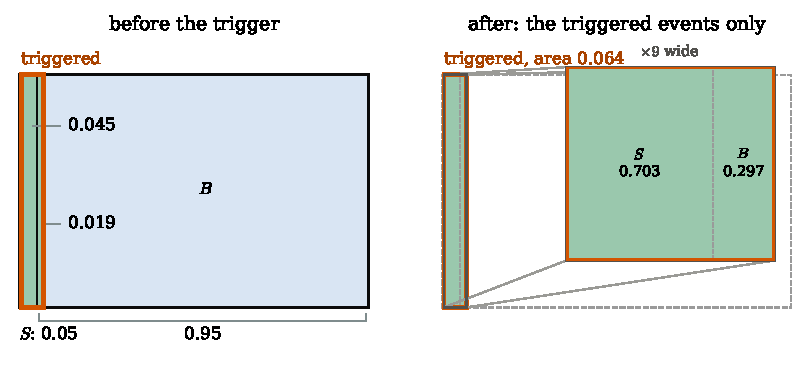
\includegraphics[width=\linewidth]{figures/ch05/area_trigger.pdf}
\caption{The trigger drawn to scale, in the picture of \cref{1a:fig:shrink}. Left:
the signal strip $S$ has width $0.05$ and the background strip $B$ width $0.95$; the
triggered events (orange outline) cover $0.90$ of the signal strip but only $0.02$
of the background strip, so the two pieces have areas $\FiveATrigJointS$ and
$\FiveATrigJointB$. The background piece covers a small share of its strip, but its
strip is nineteen times wider. Right: once we keep only triggered events, the box
is the new sample space; the inset magnifies it horizontally. Signal fills
$\FiveATrigPost$ of it.}
\label{5a:fig:trigger-area}
\end{figure}

\subsection{Drawing the boxes in Python}

The trigger figure was drawn by one short function, \pyname{box_diagram}, which
takes any list of priors and likelihoods and draws the box picture to scale. Its
geometry is the loop over strips:

\pyfile[firstline=143,lastline=156,firstnumber=143]{code/ch05/lib_area.py}{The
strips and the pieces of the evidence}\label{5a:lst:area}

Line 145 turns the priors into the positions of the strip edges, so strip $i$ runs
from the sum of the earlier priors to that sum plus its own prior. Line 149 is the
whole of the likelihood's role: the piece of $E$ in strip $i$ is as wide as the strip
times $\Prob(E\given H_i)$, and it runs the full height, so its area is prior times
likelihood. Lines 150--155 only decide where the piece sits inside its strip: it is
pushed against a neighbouring strip that also has a piece, so that the pieces join
into one box, as in \cref{1a:fig:monty-boxes}. The companion function
\pyname{posterior} in the same file computes the numbers: the joint areas are
\pyname{priors * likes}, their sum is $\Prob(E)$, and the posterior is their ratio.
The same file keeps \pyname{area_diagram}, which draws the square of
\cref{5a:fig:square} with bars. The script \pyname{code/ch05/01_area_diagrams.py}
computes the medical test, Monty Hall and the trigger, draws the trigger, and writes
the posteriors quoted above.
\section{Reallocating credibility across possibilities}
\label{5a:sec:reallocation}

We step outside in the morning and the pavement is wet. Rain? A garden sprinkler?
A burst pipe? A passer-by who spilled a drink? Each possibility has some
credibility before we look further, rain more than a spilled drink. Then we look
around. If the trees and the parked cars are wet as far as we can see, credibility
flows to rain. If the wet patch is small and there is an empty cup beside it,
credibility flows to the spilled drink, although it started low. Kruschke puts the
whole of Bayesian inference into one sentence: it is the \newterm{reallocation of
credibility across possibilities} \srcref{Kruschke}{\S2.1}.

The phrase says two things, and the square of \cref{5a:sec:shrink} makes both
exact. First, the total credibility is fixed. It is always one, shared among
possibilities that exclude each other and together cover everything we consider.
Second, credibility moves towards the possibilities that account well for what
was seen. Which ones gain? The posterior of a possibility is its prior times its
likelihood, divided by $\Prob(E)$. And $\Prob(E)$ is the average of all the
likelihoods, each weighted by its prior. So a possibility gains exactly when its
likelihood, the height of its bar in the square, is above that average. This
means any inference problem needs only three things: a list of possibilities, a
prior over the list, and, for each item, the probability of what we saw.

\begin{keyidea}[Posterior is proportional to likelihood times prior]
\[
  \Prob(H_i\given E)\;\propto\;\Prob(E\given H_i)\,\Prob(H_i),
\]
with the constant fixed by $\sum_i\Prob(H_i\given E)=1$ \mainref{p.~177, (11.2)}. Equivalently, the posterior of $H_i$ is its prior
multiplied by the factor $\Prob(E\given H_i)/\Prob(E)$, which exceeds one exactly when
$H_i$ predicted $E$ better than the prior-weighted average of all hypotheses.
\end{keyidea}

\subsection{The Bayes box}

The bookkeeping fits in a table with one row per possibility, which Lambert calls a
\newterm{Bayes box} \srcref{Lambert}{\S5.5.1}. Columns: the possibility, its prior,
its likelihood, their product, and the product divided by the column sum.

\paragraph{Example: the fish game.}
A covered bowl holds five fish, each red or white. We want the number $\alpha$ of red
fish. We pull out one fish at random and it is red: that is the event. The
candidates are the six possible bowls, $\alpha\in\{0,1,\dots,5\}$. We have no idea
beforehand, so each gets prior $\frac16$. How probable is a red fish under each
candidate? A bowl with $\alpha$ red fish out of five gives a red fish with
probability $\alpha/5$.
\begin{center}
\small
\begin{tabular}{@{}ccccc@{}}
\toprule
$\alpha$ & prior & likelihood $\alpha/5$ & prior $\times$ likelihood & posterior\\
\midrule
0 & 1/6 & 0   & 0    & 0\\
1 & 1/6 & 1/5 & 1/30 & 1/15\\
2 & 1/6 & 2/5 & 2/30 & 2/15\\
3 & 1/6 & 3/5 & 3/30 & 3/15\\
4 & 1/6 & 4/5 & 4/30 & 4/15\\
5 & 1/6 & 1   & 5/30 & 5/15\\
\midrule
sum & 1 & 3 & 15/30 $=\Prob(\text{red})$ & 1\\
\bottomrule
\end{tabular}
\end{center}
The posterior column is the product column divided by its sum, $\frac12$. The
table shows three things. First, the likelihood column sums to $3$, not to $1$:
as in \cref{5a:sec:two-directions}, a likelihood is not a distribution over the
possibilities. Second, $\alpha=0$ is eliminated, because a bowl with no red fish
cannot produce a red fish. Third, with a flat prior the posterior has the same
shape as the likelihood, here a straight line rising to $\alpha=5$. Suppose
instead we believed that the game-maker likes mixed bowls. A prior peaked at
$\alpha=2,3$ would then pull the posterior back towards the middle. The posterior
is a compromise between prior and likelihood \srcref{Lambert}{\S5.5.1},
\srcref{Kruschke}{\S5.3}.

\subsection{Elimination and exoneration}

Sherlock Holmes said: ``when you have eliminated the impossible, whatever remains,
however improbable, must be the truth''. In the Bayes box this is a likelihood of
zero. If the observation is impossible under $H_j$, then $\Prob(E\given H_j)=0$, and
that row's posterior is zero. If the other possibilities all have the same
likelihood, their posteriors are just their priors rescaled to sum to one. Kruschke
draws four suspects at $0.25$ each: rule out A, and B, C, D get $\frac13$ each;
rule out B as well, and C, D get $\frac12$; rule out C, and D gets $1$
\srcref{Kruschke}{\S2.1, Fig.~2.1}. The reverse, \emph{exoneration}, is an
observation that only one possibility can produce: then that possibility gets
credibility one and all the others are cleared \srcref{Kruschke}{Fig.~2.2}.

\paragraph{Example: the trigger path, continued.}
Recall the event of \cref{5a:sec:two-directions} that had lost its trigger flag.
One of three paths fired it: muon ($H_\mu$), calorimeter ($H_{\rm cal}$) or track
($H_{\rm trk}$). The isolated muon $E$ moved their credibility from
$(0.25,0.60,0.15)$ to $(0.745,0.128,0.128)$. Now we read the run log and find that
during this run the muon trigger was masked: it could not fire. How probable is
that log entry under each path? If the muon path fired the event, a mask is
impossible, so the probability is $0$. If either other path fired it, the mask
is certain to be in the log, so the probability is $1$. The new likelihoods
multiply the old posteriors:
\begin{align*}
  \Prob(H_\mu\given E,\text{mask})
  &\eqby{1}\frac{0\times0.745}{0\times0.745+1\times0.128+1\times0.128}=0,\\
  \Prob(H_{\rm cal}\given E,\text{mask})=\Prob(H_{\rm trk}\given E,\text{mask})
  &\eqby{2}\frac12 .
\end{align*}
\begin{explain}
  \item Bayes' theorem with the previous posterior as the new prior (justified in
        \cref{5a:sec:sequential}); the mask entry has likelihoods $(0,1,1)$.
  \item The two survivors have equal likelihood, so they keep the ratio of their
        previous credibilities, which was $1:1$.
\end{explain}
The muon path, the favourite a moment ago, is gone. Its $0.745$ has been shared
between the two survivors in proportion to what they had. \Cref{5a:fig:cred-trigger}
shows the whole sequence as bars.

\begin{figure}[htbp]
\centering
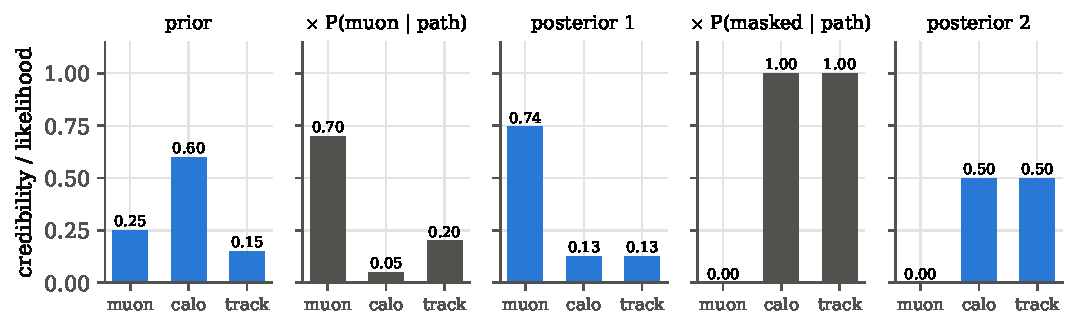
\includegraphics[width=\linewidth]{figures/ch05/credibility_trigger.pdf}
\caption{Credibility of the three trigger paths. From left: the prior (share of
recorded events); the likelihood of an isolated high-$p_T$ muon under each path; the
posterior; the likelihood of the run-log entry ``muon trigger masked''; the final
posterior. Blue bars always sum to one; grey bars need not. Each blue panel is the
previous blue panel times the grey panel, renormalised.}
\label{5a:fig:cred-trigger}
\end{figure}

\begin{pitfall}[A zero prior can never be revived]
If a possibility has prior zero, its posterior is zero whatever is observed, because
$0\times\Prob(E\given H)=0$. Lambert's example is someone so certain that the Earth
is flat that the round Earth gets prior zero; no amount of astronomical data can
then move it \srcref{Lambert}{\S5.7.1}. Truncating a prior (``the prevalence is surely
below $25\%$'') does the same to every value beyond the cut. Give every possibility
you cannot rule out on physical grounds a nonzero prior.
\end{pitfall}

\subsection{Noisy data only nudge}

Holmes' clues were decisive: each one set some likelihoods exactly to zero. Real
measurements are noisy. A noisy measurement is only somewhat more probable under one
possibility than under another, so credibility moves gradually and nothing is
ruled out.

\paragraph{Example: which ball size?}
A factory makes balls in four sizes, with nominal diameters $1,2,3,4$ (in some
unit). Inflation varies, so a ball of size $s$ has a diameter spread around $s$; take
it Gaussian with standard deviation $\sigma=1.17$.\footnote{This value reproduces
Kruschke's percentages; he does not state the spread he used.} We ordered three balls
of size $2$.

\emph{The event.} We measure the three diameters $d=(1.77,2.23,2.70)$.

\emph{The question.} Did we get what we ordered
\srcref{Kruschke}{\S2.1.1, Fig.~2.3}? Which size could have produced these three
diameters?

\emph{The candidates.} The four sizes $s=1,2,3,4$. The factory may have lost our
order, so we do not trust the label and give each size prior $\frac14$.

\emph{How probable are the data under each size?} The three diameters are
independent once the size is fixed, so the likelihood is a product of three
Gaussian densities:
\begin{align}
  p(\data\given s)
  &\eqby{1}\prod_{i=1}^3\frac{1}{\sqrt{2\pi}\,\sigma}
          \exp\!\Bigl[-\frac{(d_i-s)^2}{2\sigma^2}\Bigr]
  \eqby{2}\frac{1}{(2\pi\sigma^2)^{3/2}}
          \exp\!\Bigl[-\frac{1}{2\sigma^2}\sum_{i=1}^3(d_i-s)^2\Bigr] .
  \label{5a:eq:balls}
\end{align}
\begin{explain}
  \item Independence given $s$: the joint density is the product of the three
        single-ball densities $\Normal(d_i;s,\sigma^2)$.
  \item Collect the three exponentials into one.
\end{explain}
The prefactor is the same for every $s$, so it cancels in the posterior. Only the
sum of squared distances from the data to $s$ matters, and the smaller it is, the
larger the likelihood. The sums are $5.00$, $0.60$, $2.20$ and $9.80$ for
$s=1,2,3,4$: size $2$ is closest to the three measurements.

\emph{Only then the numbers.} With equal priors, the posterior
(\cref{5a:fig:balls}) is $\FiveABallPa$, $\FiveABallPb$, $\FiveABallPc$,
$\FiveABallPd$ for sizes $1$ to $4$. Size $2$ is the most credible, but far from
certain. Its likelihood is only $\FiveABallLRbc$ times that of size $3$, because
the spread of a single ball, $\sigma=1.17$, is larger than the distance between
sizes. No size is ruled out, since a Gaussian is never exactly zero. Size $4$ is
merely very unlikely.

\begin{figure}[htbp]
\centering
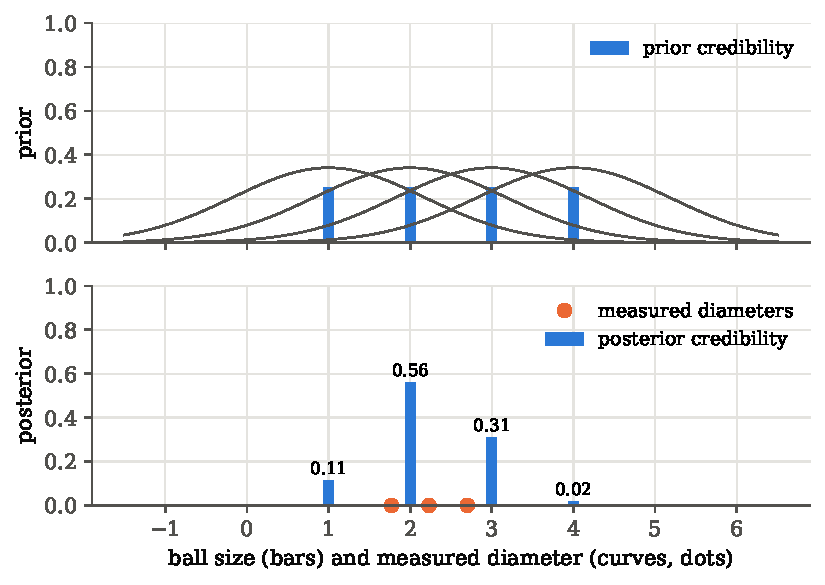
\includegraphics[width=0.78\linewidth]{figures/ch05/credibility_balls.pdf}
\caption{Top: four candidate ball sizes with equal prior credibility (bars), and the
spread of diameters each size produces (curves). Bottom: the three measured diameters
(dots on the axis) and the posterior credibility of each size. The data sit between
sizes 2 and 3, closer to 2, and the credibility moves accordingly, without ruling
anything out.}
\label{5a:fig:balls}
\end{figure}

Data analysis is exactly this, with the balls replaced by physical parameters. We
list the possible sources of the data, write down how each would produce data,
and let the data reallocate the credibility \srcref{Kruschke}{\S2.1.1}. The recipe
has the same steps in every textbook. Identify the data. Write a model that gives
the probability of the data for each possibility. Put a prior on the
possibilities. Apply Bayes' theorem. Check that the most credible possibilities
actually reproduce the data \srcref{Kruschke}{\S2.3}, \mainref{p.~176}. Repeat as
new data arrive \srcref{SeeingTheory}{p.~51}. The possibilities are usually the
values of the parameters of a model \srcref{Kruschke}{\S2.2}. When a parameter is
continuous, the row of bars becomes a density over it. Each value of the parameter, here
the ball size $s$, is then one candidate explanation of the measured data, and
its likelihood says how easily that value could have produced them; this is
parameter estimation, taken up for continuous parameters in
\cref{5b:sec:continuous}.

\subsection{Which source produced this photon?}

A gamma-ray burst goes off, and in the $100\,$s after it a gamma-ray telescope
records photons from a $10^\circ\times10^\circ$ patch of sky around it. Each photon
comes with a reconstructed direction $\bm r$ and energy $E$. Three sources can produce
a photon in this patch: the burst itself (G), a steady blazar $1.3^\circ$ away (Bz),
and the diffuse gamma-ray background spread over the whole patch (D). For each
photon we ask: which source produced it? This is the trigger-path problem again.
The candidates are the three sources, and the evidence is the photon's direction
and energy, which are continuous.

\paragraph{Priors from rates.}
Before we look at a photon's direction or energy, the probability that it came from
source $k$ is that source's share of the expected photon count in the window. We
take $30$ expected burst photons, $8$ from the blazar and $40$ from the diffuse
background, so the priors are $\FiveAGrbPriorG$, $\FiveAGrbPriorB$ and
$\FiveAGrbPriorD$. The diffuse background is the most probable source of a random
photon.

\paragraph{Likelihoods from the instrument.}
The telescope does not report a direction exactly. A photon from a point source at
$\bm r_k$ is reconstructed at $\bm r$ with a probability density given by the
\newterm{point-spread function} \unpack{the density of reconstructed directions for a
point source, here a 2-D Gaussian of width $\sigma(E)$}, which is wide at low energy
and narrow at high energy; we take $\sigma(E)=0.8^\circ\,(E/1\,\text{GeV})^{-0.8}$. The
energy of a photon from source $k$ is distributed according to that source's spectrum,
a power law $p(E\given k)\propto E^{-\gamma_k}$ with $\gamma=2.0$ for the burst,
$2.4$ for the blazar and $2.6$ for the diffuse emission. Direction and energy are
independent given the source, apart from the energy dependence of the PSF width, so
\begin{align}
  p(\bm r,E\given k)
  \eqby{1}p(E\given k)\;p(\bm r\given E,k)
  \eqby{2}
  \begin{cases}
    p(E\given k)\,\dfrac{1}{2\pi\sigma(E)^2}
      \exp\!\Bigl[-\dfrac{|\bm r-\bm r_k|^2}{2\sigma(E)^2}\Bigr],
      & k=\text{G, Bz},\\[3mm]
    p(E\given \text{D})\,\dfrac{1}{A}, & k=\text{D}.
  \end{cases}
  \label{5a:eq:grb-like}
\end{align}
\begin{explain}
  \item Product rule for densities.
  \item For a point source the direction density is the PSF centred on the source.
        For the diffuse background every direction in the patch of area $A=100\,\text{deg}^2$
        is equally likely.
\end{explain}

\paragraph{Densities as likelihoods.}
The observation ``the photon arrived exactly at $\bm r$ with exactly energy $E$'' has
probability zero under every source. What the telescope really reports is ``in a
small cell $\dd^2\bm r\,\dd E$ around $(\bm r,E)$'', and that has probability
$p(\bm r,E\given k)\,\dd^2\bm r\,\dd E$. The cell size is the same factor for every
source and cancels between the numerator and the denominator of Bayes' theorem. So
densities can stand in for probabilities as likelihoods, as long as all of them are
densities in the same variables.

\paragraph{Example: one photon.}
A photon arrives at $\bm r=(0.7^\circ,0.3^\circ)$ with $E=2\,$GeV, between the burst
and the blazar and a little closer to the blazar. At this energy the PSF width is
$\FiveAGrbSigOne^\circ$. The three likelihoods \eqref{5a:eq:grb-like} are
$\FiveAGrbLG$, $\FiveAGrbLB$ and $\FiveAGrbLD$ per $\text{deg}^2$ per GeV. Then
\begin{align*}
  \Prob(\text{G}\given\bm r,E)
  \eqby{1}\frac{\FiveAGrbPriorG\times\FiveAGrbLG}
   {\FiveAGrbPriorG\times\FiveAGrbLG+\FiveAGrbPriorB\times\FiveAGrbLB
    +\FiveAGrbPriorD\times\FiveAGrbLD}
  \eqby{2}\FiveAGrbMaG ,
\end{align*}
\begin{explain}
  \item Bayes' theorem with the three sources as the partition.
  \item Numerically, $1.84\times10^{-3}/2.28\times10^{-3}$.
\end{explain}
and likewise $\Prob(\text{Bz}\given\bm r,E)=\FiveAGrbMaB$,
$\Prob(\text{D}\given\bm r,E)=\FiveAGrbMaD$. The burst wins, and each source's
result has a plain reason. The photon is closer to the blazar, so the direction
alone slightly favours the blazar. But the burst is nearly four times brighter in
this window, which gives it the larger prior, and its harder spectrum makes a
$2\,$GeV photon more probable. The product of prior and likelihood is therefore
largest for the burst. The diffuse background was the most probable source before
we looked at the photon. It loses because its likelihood is spread evenly over the
whole patch: it predicts \emph{this} direction no better than any other.

\Cref{5a:fig:grb-sky} does this for every photon of one simulated window. Photons near
the burst are dark (almost surely burst photons), photons far from both point sources
are pale (mostly background), and photons between the two point sources are shared.
A soft photon far out, at $(-3^\circ,2^\circ)$ with $E=0.3\,$GeV, still has
$\Prob(\text{G}\given\bm r,E)=\FiveAGrbMbG$: at $0.3\,$GeV the PSF is about
$2^\circ$ wide, so the burst can put a photon there.

\begin{figure}[htbp]
\centering
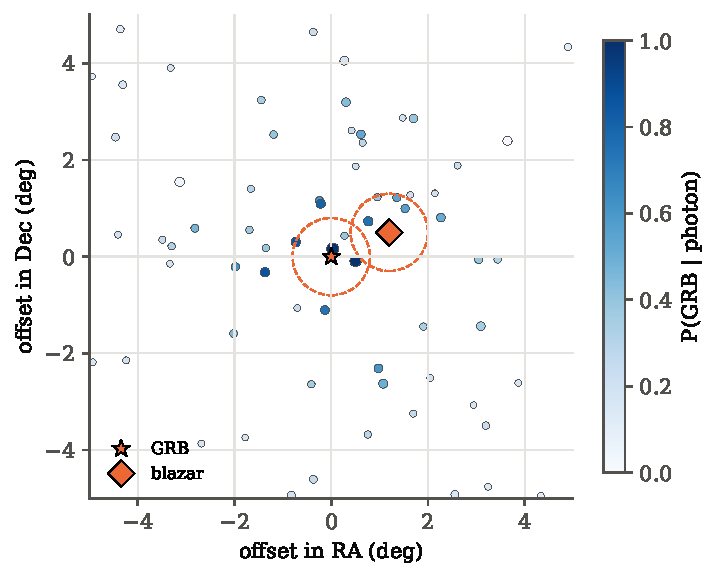
\includegraphics[width=0.68\linewidth]{figures/ch05/grb_sky.pdf}
\caption{One simulated $100\,$s window of photons around a gamma-ray burst (star),
with a blazar nearby (diamond) and a diffuse background. Each dot is a photon, larger
for higher energy, shaded by its posterior probability of having come from the
burst. The dashed circles have the radius of the point-spread function at $1\,$GeV.
Dark dots cluster on the burst; photons far from both point sources are pale.}
\label{5a:fig:grb-sky}
\end{figure}

\pyfile[firstline=56,lastline=67,firstnumber=56]{code/ch05/03_grb_source.py}{Posterior
source probabilities for a photon}

Lines 58--60 are the three cases of \eqref{5a:eq:grb-like}, one column per source.
Line 66 multiplies each column by its prior (the expected counts; their common
normalisation cancels), and line 67 divides by the sum over sources. It works on a
whole array of photons at once. Adding the burst column over all photons of the
window gives $\FiveAGrbNest$, an estimate of the number of burst photons; the
simulation actually contained $\FiveAGrbNtrue$ of the $\FiveAGrbNphot$. Such
per-photon source probabilities are used in gamma-ray astronomy to weight photons
when searching for pulsations or transients, so that background photons dilute the
signal less.
\section{Odds and the likelihood ratio: evidence as a multiplier}
\label{5a:sec:odds}

A search for a rare process uses a boosted decision tree, a classifier that gives
every event a score $x$ between $0$ and $1$. Signal events tend to score high,
background events low, and both distributions are known from simulation. Before we
look at its score, an event is signal with probability $\pi$, the signal fraction of
the sample. Then one event scores $x=0.9$. How probable is it that this event is
signal? And how would the answer change in another analysis with the same classifier
but a hundred times less signal?

The answer splits into two factors. One depends only on the classifier and the
score. The other depends only on the sample. The second question then needs no new
work: we keep the first factor and change the second. This split is the odds form
of Bayes' theorem, and it gives the simplest working rule for the question
``which hypothesis produced this?''.

\subsection{Odds}

The \newterm{odds} on a hypothesis are its probability divided by the probability of
its negation, $O(H)=\Prob(H)/\Prob(\neg H)$. Odds and probability carry the same
information:
\begin{equation}
  O=\frac{p}{1-p}
  \qquad\Longleftrightarrow\qquad
  p=\frac{O}{1+O} .
  \label{5a:eq:odds-prob}
\end{equation}
A probability of $\frac12$ is odds $1$ (``evens''), $0.9$ is odds $9$, $0.01$ is odds
$1/99$. More generally, for any two hypotheses $H_1$, $H_2$ in a partition, the ratio
$\Prob(H_1)/\Prob(H_2)$ is the odds of $H_1$ against $H_2$.

How do the odds of $H_1$ against $H_2$ change when we observe $E$? Write Bayes'
theorem \eqref{5a:eq:bayes} for $H_1$ and for $H_2$ and divide:
\begin{align}
  \frac{\Prob(H_1\given E)}{\Prob(H_2\given E)}
  &\eqby{1}\frac{\Prob(E\given H_1)\,\Prob(H_1)/\Prob(E)}
               {\Prob(E\given H_2)\,\Prob(H_2)/\Prob(E)}
  \eqby{2}\underbrace{\frac{\Prob(E\given H_1)}{\Prob(E\given H_2)}}_{\text{likelihood ratio}}
   \times\underbrace{\frac{\Prob(H_1)}{\Prob(H_2)}}_{\text{prior odds}} .
  \label{5a:eq:odds}
\end{align}
\begin{explain}
  \item Bayes' theorem in numerator and denominator.
  \item The evidence $\Prob(E)$ is common to both and cancels.
\end{explain}
We write $\Lambda$ for the likelihood ratio.

\begin{keyidea}[Evidence multiplies odds]
\[
  \text{posterior odds}=\Lambda\times\text{prior odds},
  \qquad
  \Lambda=\frac{\Prob(E\given H_1)}{\Prob(E\given H_2)} .
\]
The \newterm{likelihood ratio} $\Lambda$ is everything the observation has to say
about $H_1$ versus $H_2$. It does not involve the priors, it does not involve any
other hypothesis, and it does not need $\Prob(E)$.
\end{keyidea}

In the square of \cref{5a:sec:shrink} every factor of \eqref{5a:eq:odds} is a ratio of
shapes. The prior odds are the ratio of the two strip \emph{widths}. The likelihood
ratio is the ratio of the two bar \emph{heights}. Their product, width ratio times
height ratio, is the ratio of the two surviving \emph{areas}, which is the posterior
odds. Take the medical test of \cref{5a:fig:medical}. The strip widths are
$\Prob(D)=0.01$ and $\Prob(D^c)=0.99$, a ratio of $1:99$. The positive result covers
$0.95$ of the disease strip and $0.10$ of the healthy one, a likelihood ratio of
$9.5:1$. So the surviving areas are in the ratio $9.5:99\approx1:10.4$, and the
posterior probability is $1/11.4\approx0.088$ by \eqref{5a:eq:odds-prob}. The test
is good evidence, a factor of $9.5$, but it is applied to odds that started at one
to ninety-nine.

\subsection{Evidence adds in logarithms}

Take logarithms of \eqref{5a:eq:odds}. Products become sums:
\begin{equation}
  \log O(H_1{:}H_2\given E)=\log\Lambda+\log O(H_1{:}H_2) .
  \label{5a:eq:logodds}
\end{equation}
So each piece of evidence \emph{adds} its log likelihood ratio to the log odds. We
call $\log\Lambda$ the \emph{weight of evidence}. A convenient unit is the
\newterm{decibel}: $10\log_{10}$ of the odds, the same unit physicists use for the
gains along an amplifier chain. Odds of $1:99$ are $-20\,$dB, evens are $0\,$dB,
odds of $99:1$ are $+20\,$dB. A positive medical test adds
$10\log_{10}9.5=+9.8\,$dB. One positive test takes the patient from $-20.0\,$dB to
$-10.2\,$dB, which is odds $0.096$ and probability $0.088$. Suppose a second
positive test is taken, independent of the first \emph{given} the disease status
(a condition examined in \cref{5a:sec:sequential}). It adds another $9.8\,$dB, to
$-0.4\,$dB, probability $0.48$. A third takes it to $+9.4\,$dB, probability $0.90$
(\cref{5a:fig:decibels}).

\begin{figure}[htbp]
\centering
\begin{tikzpicture}[font=\small,x=0.28cm]
  \draw[->] (-24,0) -- (24,0) node[right] {dB};
  \foreach \t in {-20,-10,0,10,20} {
    \draw (\t,0.12) -- (\t,-0.12) node[below,font=\footnotesize] {$\t$};
  }
  \node[font=\footnotesize,align=center,anchor=north] at (-20,-0.75) {odds $1{:}99$};
  \node[font=\footnotesize,align=center,anchor=north] at (0,-0.75) {evens};
  \node[font=\footnotesize,align=center,anchor=north] at (20,-0.75) {odds $99{:}1$};
  \foreach \x/\p/\n in {-19.96/0.010/prior, -10.18/0.088/1 test, -0.40/0.48/2 tests, 9.38/0.90/3 tests}{
    \fill[formblue] (\x,0) circle (2.2pt);
    \node[anchor=south,font=\footnotesize,align=center] at (\x,1.05) {\n\\ $p=\p$};
  }
  \foreach \a/\b in {-19.96/-10.18, -10.18/-0.40, -0.40/9.38}{
    \draw[->,thick,tangentgreen] (\a,0.12) to[out=60,in=120] (\b,0.12);
  }
  \node[font=\footnotesize,tangentgreen!60!black,anchor=west] at (11,0.55)
    {each green step: $+9.8$ dB};
\end{tikzpicture}
\caption{The medical test as a walk on a scale of log odds. The prior, one person in a
hundred, sits at $-20\,$dB. Each positive result from an independent test adds the
same weight of evidence, $10\log_{10}9.5\approx9.8\,$dB. The probability above each
dot follows from the odds by $p=O/(1+O)$: three positive tests are needed before the
disease becomes the likely explanation.}
\label{5a:fig:decibels}
\end{figure}

The additive form explains two habits of practising physicists. First, analyses
add log likelihoods rather than multiply likelihoods, because independent pieces of
evidence add in logarithms. Second, ``how strong is this evidence?'' has an answer
that does not depend on the prior: $\log\Lambda$. Whether it is strong \emph{enough} depends on where the
prior odds started. A $+10\,$dB piece of evidence decides a question that started at
evens, and barely dents one that started at $-40\,$dB.

\subsection{Signal or background, given a classifier score}

Back to the boosted decision tree of the opening, which gives each event a score
$x$ between $0$ and $1$, and to the question: given one event's score, is it
signal ($S$) or background ($B$)? Suppose the simulation shows that signal scores follow the
density $f_S(x)=30\,x^4(1-x)$ and background scores the density
$f_B(x)=30\,x(1-x)^4$ on $[0,1]$ (\cref{5a:fig:bdt}, left). Both are Beta densities,
$\mathrm{Beta}(5,2)$ and $\mathrm{Beta}(2,5)$; all we need is that each integrates to
one, which the factor $30$ ensures. The evidence is the score of one event, a
continuous quantity, so the likelihoods are densities, and the cell $\dd x$ cancels in
the ratio exactly as the cell $\dd^2\bm r\,\dd E$ did for the photon in
\cref{5a:sec:reallocation}. The likelihood ratio is
\begin{align}
  \Lambda(x)
  &\eqby{1}\frac{f_S(x)}{f_B(x)}
  \eqby{2}\frac{30\,x^4(1-x)}{30\,x(1-x)^4}
  \eqby{3}\Bigl(\frac{x}{1-x}\Bigr)^{3} .
  \label{5a:eq:bdt-lr}
\end{align}
\begin{explain}
  \item Likelihood ratio of signal to background for the observed score.
  \item The two densities.
  \item Cancel $30$, one power of $x$ and one power of $(1-x)$.
\end{explain}
With prior odds $\pi/(1-\pi)$, the posterior odds are
$\Lambda(x)\,\pi/(1-\pi)$. In logarithms, with the \newterm{logit}
$\operatorname{logit}p=\ln[p/(1-p)]$ \unpack{the natural log of the odds},
\begin{equation}
  \operatorname{logit}\Prob(S\given x)=\operatorname{logit}\pi+3\operatorname{logit}x .
  \label{5a:eq:bdt-logit}
\end{equation}
This is the split promised at the start. The score contributes a term,
$3\operatorname{logit}x$, that depends only on the classifier. The sample
contributes a term, $\operatorname{logit}\pi$, that depends only on the signal
fraction $\pi$.

\paragraph{Example: the same score in two analyses.}
For $x=0.9$ the likelihood ratio is $9^3=729$. With $\pi=0.01$ the prior odds are
$1/99$, the posterior odds $729/99=7.36$, and
\begin{align*}
  \Prob(S\given x=0.9)\eqby{1}\frac{7.36}{1+7.36}=\FiveABdtPostNine .
\end{align*}
\begin{explain}
  \item Posterior odds converted to a probability by \eqref{5a:eq:odds-prob}.
\end{explain}
In the analysis with a hundred times less signal, $\pi=10^{-4}$, the likelihood
ratio is unchanged and only the prior odds change. The same score gives posterior
odds $729/9999=0.073$, so $\Prob(S\given x=0.9)=\FiveABdtPostNineTiny$. Same event,
same classifier, and now it is probably background. A score of $0.8$ is weaker
evidence, $\Lambda=4^3=64$, and gives only $\FiveABdtPostEight$ at $\pi=0.01$. The score
at which an event becomes more likely signal than not, $\Prob(S\given x)=\frac12$, is
where $3\operatorname{logit}x=-\operatorname{logit}\pi$: $x_{1/2}=\FiveABdtHalfOne$ for
$\pi=0.01$ and $\FiveABdtHalfTiny$ for $\pi=10^{-4}$ (\cref{5a:fig:bdt}, right).

\begin{figure}[htbp]
\centering
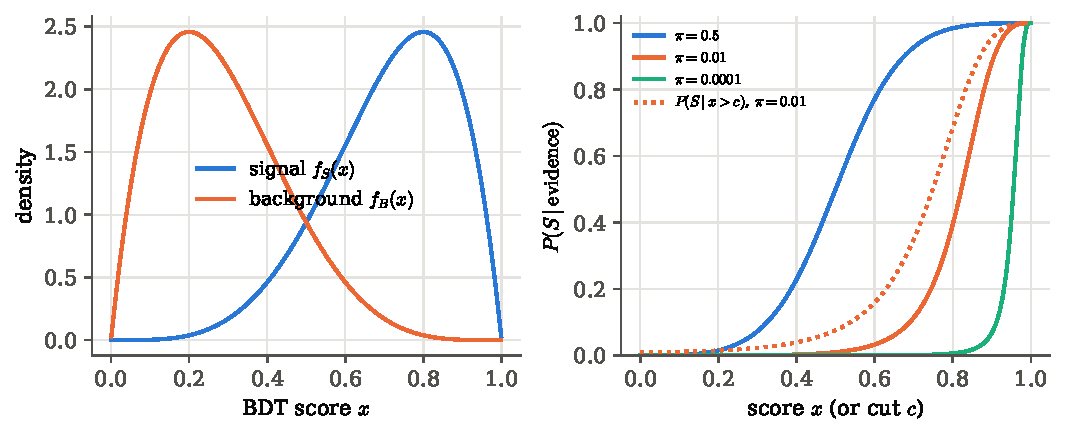
\includegraphics[width=\linewidth]{figures/ch05/bdt_posterior.pdf}
\caption{Left: the score densities of signal and background. Right: the probability
that an event is signal given its score $x$, for three signal fractions $\pi$ (solid).
The curves are the same likelihood ratio combined with different prior odds, so they
are shifted copies of one another on the logit scale. The dotted curve is a different
question: the signal fraction of the whole sample with $x>c$, plotted against the cut
$c$, for $\pi=0.01$.}
\label{5a:fig:bdt}
\end{figure}

\paragraph{Checking it by selection.}
We can check the formula without algebra, because conditioning on an observation
is the same as selecting the events that show it (\cref{ch:01}). The script \pyname{code/ch05/04_bdt_posterior.py} generates $10^7$ events
with $\pi=0.01$, draws each event's score from $f_S$ or $f_B$, keeps the
$\FiveABdtNsel$ events with $|x-0.9|<0.005$, and counts the signal among them: the
fraction is $\FiveABdtMC\pm\FiveABdtMCerr$, against $\FiveABdtPostNine$ from
\eqref{5a:eq:bdt-logit}. Bayes' theorem is the statement of what this selection
returns.

\subsection{Be exact about what you observed}

A score and a cut are different observations, and they give different answers.
The dotted curve in \cref{5a:fig:bdt} shows the cut. Suppose we do not look at each
event's score but select all events with $x>c$ and ask for the signal fraction of
the selected sample, its \newterm{purity}. The observed event is now
``$x>c$'', whose probability under each hypothesis is an efficiency,
$\varepsilon_S(c)=\int_c^1f_S\,\dd x$ and $\varepsilon_B(c)=\int_c^1f_B\,\dd x$. For
$c=0.8$ these are $\FiveABdtEffS$ and $\FiveABdtEffB$, so
\begin{align*}
  \Lambda(x>0.8)\eqby{1}\frac{\varepsilon_S}{\varepsilon_B}=\FiveABdtCutLR,
  \qquad
  \Prob(S\given x>0.8)\eqby{2}\FiveABdtCutPur .
\end{align*}
\begin{explain}
  \item The likelihood ratio of the event ``$x>0.8$'' is the ratio of the probabilities
        of that event, the two efficiencies.
  \item Posterior odds $\FiveABdtCutLR/99$, converted with \eqref{5a:eq:odds-prob}.
\end{explain}
This is much larger than $\Prob(S\given x=0.8)=\FiveABdtPostEight$. Why? The
selected sample contains all the events with $x$ between $0.8$ and $1$. Most of
them score well above $0.8$, and their scores are much stronger evidence. An event
that sits exactly at the cut is among the \emph{least} signal-like in the sample.
Bayes' theorem conditions on exactly the statement we say we know, nothing more. ``The score is
$0.8$'' and ``the score is above $0.8$'' are different observations with different
likelihood ratios, and mixing them is a common error in quoting per-event
probabilities.

\paragraph{Why the likelihood ratio is the right score.}
For two hypotheses, \eqref{5a:eq:odds} says that the posterior depends on the data
only through $\Lambda$. Any two events with the same $\Lambda$ are equally
signal-like, whatever else differs between them. This is the Bayesian face of the
Neyman--Pearson lemma of \cref{ch:04}: the most powerful selection at any background
rejection is a cut on $\Lambda$. A classifier whose score is a monotonic function of
$\Lambda$ is already optimal, and our score is one, since $(x/(1-x))^3$ increases with
$x$.

\begin{inpractice}[The likelihood-ratio trick]
A classifier trained with balanced samples of simulated signal and background, and a
loss such as the cross-entropy, learns in the limit of enough data and flexibility to
output $s(x)=\Prob(S\given x)$ at $\pi=\frac12$, that is
$s=\Lambda/(1+\Lambda)$. Then $\Lambda(x)=s/(1-s)$ is recovered from the output, and
\eqref{5a:eq:odds} converts it to the posterior for the actual signal fraction of any
sample. The same trick turns classifiers into estimators of likelihood ratios between
two parameter points, which is how simulation-based inference compares hypotheses
whose likelihoods cannot be written down.
\end{inpractice}
\section{Sequential updating: yesterday's posterior is today's prior}
\label{5a:sec:sequential}

We find a coin on the pavement and want to know how biased it is. We toss it once and
it lands heads. It is tempting to say that one toss tells us nothing. It tells us
something: the coin is not two-tailed, a possibility that was open a moment ago, and
coins that favour heads are now a little more credible than before
\srcref{SeeingTheory}{p.~53}. We toss again, and again. Each toss should move our
belief a little more, starting from wherever the previous tosses left it. Is that
legitimate? Do we get the same answer as if we had waited for all the tosses and
analysed them at once? And does it matter in which order the tosses came?

\subsection{The update rule}

Let $D_1$ be the first piece of data and $D_2$ the second. Everything we know after
both is $\Prob(H\given D_1,D_2)$. The question is whether we can reach it in two
steps: first update on $D_1$, then update the result on $D_2$. To see, apply Bayes'
theorem to $D_2$ alone, with $D_1$ added to the background information of every
probability:
\begin{align}
  \Prob(H\given D_1,D_2)
  &\eqby{1}\frac{\Prob(D_2\given H,D_1)\;\Prob(H\given D_1)}{\Prob(D_2\given D_1)}
  \label{5a:eq:seq-general}\\
  &\eqby{2}\frac{\Prob(D_2\given H)\;\Prob(H\given D_1)}
               {\sum_j\Prob(D_2\given H_j)\,\Prob(H_j\given D_1)} .
  \label{5a:eq:seq}
\end{align}
\begin{explain}
  \item Bayes' theorem \eqref{5a:eq:bayes-xy} with $X=H$, $Y=D_2$ and background
        information $I$ replaced by ``$I$ and $D_1$''. Every rule of probability holds
        with extra information in the conditioning, since $\Prob(\cdot\given D_1)$ is
        itself a probability \srcref{Sivia}{\S1.2}.
  \item \emph{If} $D_2$ is independent of $D_1$ given each hypothesis,
        $\Prob(D_2\given H_j,D_1)=\Prob(D_2\given H_j)$. The denominator is then the
        marginalisation \eqref{5a:eq:marg} over the $H_j$, done inside
        $\Prob(\cdot\given D_1)$.
\end{explain}
Line \eqref{5a:eq:seq} is Bayes' theorem for $D_2$ alone, with the posterior after
$D_1$ in the place of the prior. So the answer is yes: the posterior of one step is
the prior of the next. This needs one condition, that the data are
\newterm{conditionally independent} \unpack{independent once the hypothesis is
fixed, although not independent when the hypothesis is unknown}. Line
\eqref{5a:eq:seq-general} needs no assumption at all.

\paragraph{The order does not matter.}
Doing $D_2$ first and $D_1$ second must give the same answer. Both routes compute
the probability of $H$ given the \emph{single} statement ``$D_1$ and $D_2$'', and
``$D_1$ and $D_2$'' is the same statement as ``$D_2$ and $D_1$''. The formula shows
the same thing. Under conditional independence, doing the two updates in one go
gives \srcref{Kruschke}{\S5.2.1}
\begin{align*}
  \Prob(H\given D_1,D_2)
  &\eqby{1}\frac{\Prob(D_1,D_2\given H)\,\Prob(H)}{\sum_j\Prob(D_1,D_2\given H_j)\,\Prob(H_j)}
  \eqby{2}\frac{\Prob(D_1\given H)\,\Prob(D_2\given H)\,\Prob(H)}
              {\sum_j\Prob(D_1\given H_j)\,\Prob(D_2\given H_j)\,\Prob(H_j)}\\
  &\eqby{3}\frac{\Prob(D_2\given H)\,\Prob(D_1\given H)\,\Prob(H)}
              {\sum_j\Prob(D_2\given H_j)\,\Prob(D_1\given H_j)\,\Prob(H_j)}
  \eqby{4}\Prob(H\given D_2,D_1) .
\end{align*}
\begin{explain}
  \item Bayes' theorem for the combined data.
  \item Conditional independence: the joint likelihood is the product.
  \item Multiplication of numbers commutes.
  \item Bayes' theorem read backwards, with the data in the other order.
\end{explain}
Updating one datum at a time computes the same product in stages. Each stage
multiplies by one likelihood and renormalises. Renormalising early instead of at
the end changes nothing, because a constant factor cancels in the ratio.

\begin{keyidea}[Sequential updating]
For data that are independent given the hypothesis, updating one datum at a time,
each posterior serving as the next prior, gives exactly the posterior of updating
with all the data at once, in any order. In log-odds form each datum simply adds its
log likelihood ratio. Without conditional independence the general rule
\eqref{5a:eq:seq-general} still holds, and the order still does not matter, but each
datum's likelihood must then be conditioned on the data before it.
\end{keyidea}

\subsection{The sample space, toss by toss}

A coin is either fair, $\Prob(\text{heads})=0.5$, or biased, $\Prob(\text{heads})=0.8$,
and we give each prior $\frac12$. We toss it four times and see H, H, T, H.
\Cref{5a:fig:shrink-seq} shows two ways of watching the sample space shrink.

The top row keeps the original sample space, drawn as in \cref{1a:fig:shrink}: two
strips of width $\frac12$, the biased coin on the left. After each toss, the
evidence ``the tosses so far'' is a box, and the part of each strip that it covers is
the part that survives. The share of the strip it covers is the probability of the
whole sequence so far under that coin: $0.8$, $0.64$, $0.128$,
$0.1024$ for the biased coin and $0.5$, $0.25$, $0.125$, $0.0625$ for the fair one. The
box only ever shrinks. After all four tosses its area is
\begin{align*}
  \Prob(\text{HHTH})
  \eqby{1}\tfrac12\times0.8^3\times0.2+\tfrac12\times0.5^4
  =0.0512+0.03125=\FiveASeqArea ,
\end{align*}
\begin{explain}
  \item Marginalisation over the two coins, with the product of the four toss
        probabilities (conditionally independent given the coin) as each likelihood.
\end{explain}
the probability, before any toss, of seeing exactly this sequence.

The bottom row blows the surviving box back up to area one after each toss. The
dividing line is then the current posterior, which is the prior for the next toss:
$0.5$, then $\FiveASeqPa$ after H, $\FiveASeqPb$ after HH, $\FiveASeqPc$ after HHT, and
$\FiveASeqPd$ after HHTH. The box in each rescaled panel is the next toss, covering a share of each strip
equal to its likelihood. A head is $0.8/0.5=1.6$ times more likely from the biased coin and moves
the line right; the tail is $0.2/0.5=0.4$ times as likely and moves it back left.
Both rows give the same final posterior,
$0.0512/\FiveASeqArea=\FiveASeqPd$: renormalising at every step or only at the end is
the same calculation.

\begin{figure}[htbp]
\centering
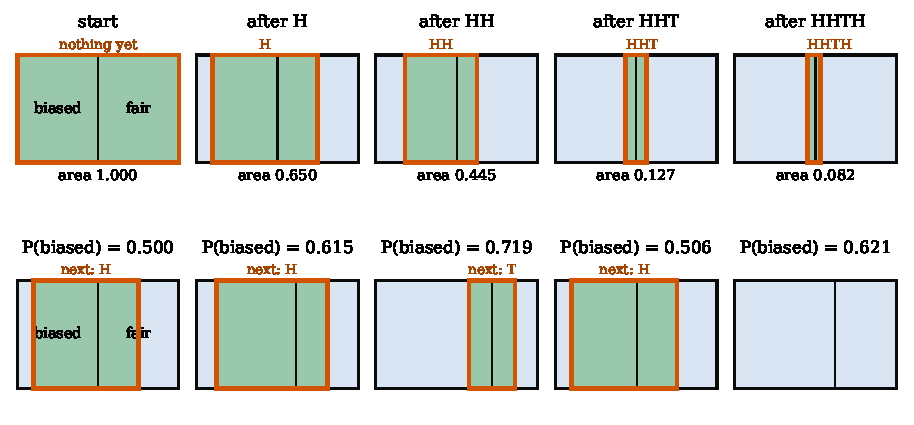
\includegraphics[width=\linewidth]{figures/ch05/shrinking_sequence.pdf}
\caption{The sample space shrinking toss by toss, for a biased coin (left strip)
against a fair one (right strip), drawn to scale as in \cref{1a:fig:shrink}. Top row:
the original sample space, with the tosses so far as a box (orange outline) that
covers $0.8$ or $0.5$ of each strip per head and $0.2$ or $0.5$ per tail; the number
under each panel is the area of the box, the probability of the sequence so far.
Bottom row: the surviving box rescaled to area one, so that the dividing line is the
current posterior of the biased coin; the box drawn in it is the next toss (the last
panel has no next toss).}
\label{5a:fig:shrink-seq}
\end{figure}

\subsection{A grid of biases}

Real coins are not limited to two types. The real question is: what is the coin's
probability of heads $\theta$, which could be anywhere in $[0,1]$? Kruschke's
answer is to allow a grid of candidate values, say
$\theta_j\in\{0,0.01,\dots,1\}$, as if a factory made coins of 101 types, and to
treat each $\theta_j$ as one hypothesis \srcref{Kruschke}{\S5.3}. A single toss $y$ ($y=1$ for heads, $0$ for tails) has the
Bernoulli likelihood \srcref{Kruschke}{(5.10)}
\begin{equation}
  \Prob(y\given\theta_j)=\theta_j^{\,y}(1-\theta_j)^{1-y},
  \label{5a:eq:bernoulli}
\end{equation}
which is $\theta_j$ for a head and $1-\theta_j$ for a tail. Updating is then one line of
code:

\pyfile[firstline=34,lastline=37,firstnumber=34]{code/ch05/05_coin_grid.py}{One toss:
multiply by the likelihood on the grid and renormalise}

Line 36 multiplies the whole array of credibilities by the array of likelihoods, one
value per grid point, and line 37 divides by the sum, the discrete evidence. This is the
Bayes box of \cref{5a:sec:reallocation} with 101 rows, recomputed after each toss.

The main lesson of \cref{5a:fig:coin-grid} is that with few data the prior matters,
and with many data it hardly does. The figure follows $50$ tosses of a coin with
true $\theta=0.3$, which produced $\FiveACoinHeads$ heads. It starts from two
priors. One is flat. The other is triangular, with its peak at $\frac12$ and zero
at $0$ and $1$; it encodes the belief that most coins are roughly fair.

Each toss acts in a way we can predict. After one tail, the flat-prior posterior
is the straight line $1-\theta$, because the likelihood of a tail is $1-\theta$.
The coin that always lands heads, $\theta=1$, is ruled out. After the first head,
$\theta=0$ is ruled out too. As tosses accumulate, the posterior narrows around
the observed fraction of heads. The two posteriors move towards each other, and
after $50$ tosses they nearly coincide; the flat-prior posterior has mean
$\FiveACoinPostMean$. So with few data the posterior is a compromise between prior
and likelihood, and with many the likelihood dominates
\srcref{Kruschke}{\S5.3.1--5.3.2}. Kruschke's numbers show the same thing on a grid
of $1001$ values with the triangular prior \srcref{Kruschke}{Fig.~5.2}. One head in
$4$ tosses gives a posterior mode of $\FiveACoinModeFour$, pulled far from the
observed fraction $0.25$ towards the prior's peak. Ten heads in $40$ tosses give
$\FiveACoinModeForty$, close to $0.25$.

\begin{figure}[htbp]
\centering
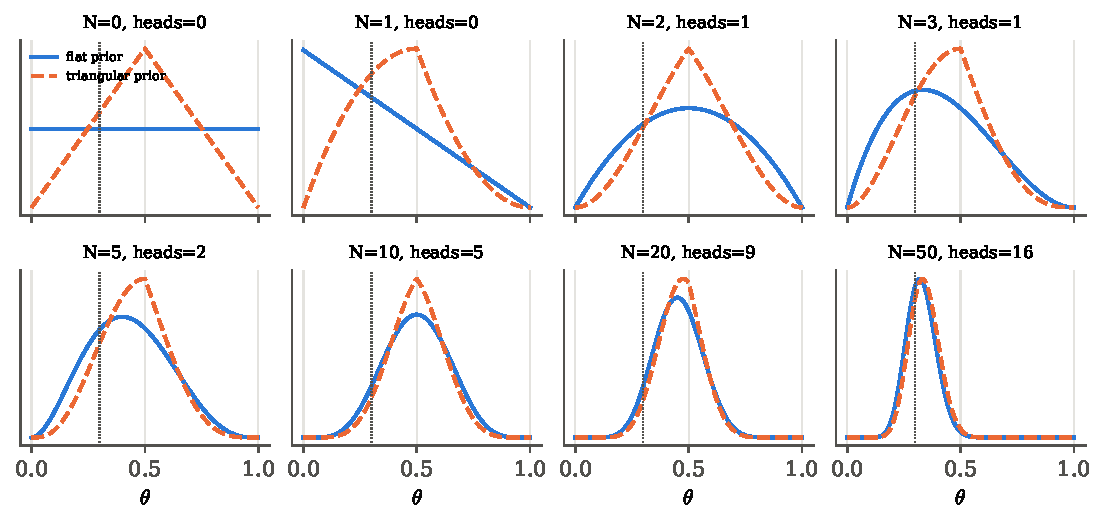
\includegraphics[width=\linewidth]{figures/ch05/coin_grid_panels.pdf}
\caption{Credibility of $101$ candidate biases $\theta$ after $N$ tosses of a coin whose
true bias is $0.3$ (dotted line), starting from a flat prior (solid) and from a
triangular prior peaked at $\frac12$ (dashed). Early on the two posteriors differ,
because the data are few; by $N=50$ both are narrow and nearly identical, centred near
the observed fraction of heads.}
\label{5a:fig:coin-grid}
\end{figure}

The script also checks the order claim numerically. It updates the flat prior with the
same $50$ tosses in $1000$ random orders and compares each result with the batch
posterior $\propto\theta^{z}(1-\theta)^{N-z}$ computed in one step ($z$ heads in $N$
tosses, \srcref{Kruschke}{(5.11)}). The largest difference at any grid point is
$\FiveACoinMaxDiff$, the size of floating-point rounding.

\subsection{Evidence accumulates as a random walk}

Return to two hypotheses, now a fair coin ($\theta_0=0.5$) against a biased one
($\theta_1=0.7$), with prior odds $1$. By \eqref{5a:eq:logodds} the $\log_{10}$ odds of
biased against fair add $\log_{10}(0.7/0.5)=\FiveACoinLRh$ for each head and
$\log_{10}(0.3/0.5)=\FiveACoinLRt$ for each tail. The log odds perform a random walk
(\cref{5a:fig:logodds}). If the coin really is biased, the average step per toss is
\begin{align}
  \E[\text{step}\given\theta_1]
  \eqby{1}\theta_1\log\frac{\theta_1}{\theta_0}+(1-\theta_1)\log\frac{1-\theta_1}{1-\theta_0}
  \equiv D_{\rm KL}(\theta_1\Vert\theta_0) ,
  \label{5a:eq:kl}
\end{align}
\begin{explain}
  \item A head, with probability $\theta_1$, contributes $\log(\theta_1/\theta_0)$; a
        tail, with probability $1-\theta_1$, contributes
        $\log[(1-\theta_1)/(1-\theta_0)]$.
\end{explain}
This average step is the \newterm{Kullback--Leibler divergence} between the two
coins \unpack{the average log likelihood ratio in favour of the true distribution;
in statistical mechanics it is the relative entropy}. It is never negative, and it
is zero only if the two coins are the same. So the walk drifts towards the truth,
whichever coin is true. The rate is $\FiveACoinKLone$ in $\log_{10}$ per toss when
the biased coin is true, and $\FiveACoinKLzero$ when the fair coin is true.
Reaching odds of $100:1$, which is $2$ in $\log_{10}$, therefore takes about
$2/\FiveACoinKLone\approx56$ tosses on average, with large scatter from one
sequence to the next. The more alike the two hypotheses, the smaller the divergence and the longer
the wait: telling apart two nearly identical coins, like two nearly identical
cosmologies, needs a lot of data.

\begin{figure}[htbp]
\centering
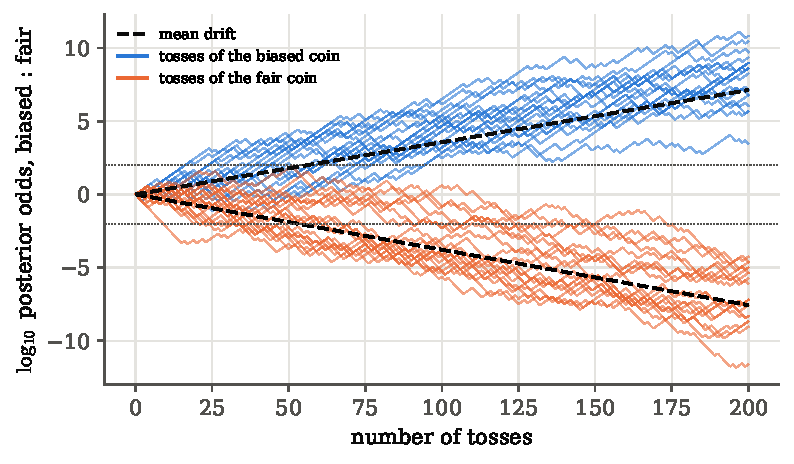
\includegraphics[width=0.82\linewidth]{figures/ch05/coin_logodds.pdf}
\caption{Log posterior odds of ``biased ($\theta=0.7$)'' against ``fair'' along $20$
simulated sequences of $200$ tosses from each coin, starting at odds $1$. Every head
steps up, every tail steps down. Sequences from the biased coin (blue) drift upward and
those from the fair coin (orange) downward, each at the rate given by a
Kullback--Leibler divergence (dashed lines). The dotted lines mark odds of $100:1$ each
way.}
\label{5a:fig:logodds}
\end{figure}

\subsection{When the data are not independent given the hypothesis}

Conditional independence is an assumption about how the data are produced, and it
can fail. When it fails, repeated evidence is worth less than the product of its
parts. Take the medical test again (prevalence $0.01$, $\Prob(+\given D)=0.95$,
$\Prob(+\given D^c)=0.10$), and suppose its false positives have two causes. Half of
them come from a harmless antibody that $5\%$ of healthy people carry, and it makes
the test positive every time. The other half are random, and happen to the other
healthy people with probability $r=0.05/0.95$ per test. The single-test false
positive rate is still $0.05+0.95\,r=0.10$. But for a healthy person two positive
tests in a row are now much more likely than $0.10^2$:
\begin{align*}
  \Prob({+}{+}\given D^c)
  \eqby{1}0.05\times1+0.95\times r^2
  =0.05+0.95\times0.00277=0.0526 .
\end{align*}
\begin{explain}
  \item Split the healthy population into antibody carriers (both tests positive
        for sure) and the others (two independent random false positives).
\end{explain}
For the diseased we keep independent tests, $\Prob({+}{+}\given D)=0.95^2=0.9025$. The
likelihood ratio of two positives is $0.9025/0.0526=17.1$, not $9.5^2=90$. Starting
from odds $1/99$, the posterior odds are $0.173$ and $\Prob(D\given{+}{+})=0.15$,
where the naive product would have given $0.48$. The second test is weaker evidence
because a large part of what made the first test positive in a healthy person repeats
itself.

\begin{pitfall}[Correlated data are not independent evidence]
Multiplying likelihoods, or adding log likelihood ratios, assumes that the data are
independent \emph{given} each hypothesis. Repeated measurements that share a
calibration offset, a common background mismodelling, overlapping sky patches or the
same patient-specific cause are correlated even given the hypothesis. Treating them as
independent double-counts the shared part and makes the evidence look far stronger
than it is. The remedy is to write the joint likelihood with its correlations, as a
multivariate Gaussian with a full covariance matrix $\Cmat$ does for Gaussian data.
\end{pitfall}

\subsection{Screening for breast cancer, test by test}
\label{5a:sec:screening}

A woman of fifty with no symptoms goes for a routine screening mammogram. The result
is positive. She is recalled for an ultrasound, and if that is positive too, for a
biopsy. After each result she, and her doctor, want to know one thing: how probable is
it now that she has cancer? We use round numbers of the right size for this age group,
illustrative rather than taken from a particular study: a \newterm{prevalence}
\unpack{the fraction of women screened at this age who have breast cancer at the time
of screening} of $1\%$; for the mammogram a sensitivity of $0.87$ and a specificity of
$0.90$; for the ultrasound $0.80$ and $0.90$; for the biopsy $0.95$ and $0.99$.
Sensitivity is $\Prob(+\given C)$, the chance that the test is positive if she has
cancer ($C$); specificity is $\Prob(-\given C^c)$, the chance that it is negative if
she has none ($C^c$).

There are two hypotheses throughout, $C$ and $C^c$, and each test redistributes the
whole unit of probability between them. The posterior after one test is the prior for
the next, by \eqref{5a:eq:seq}, as long as the tests are conditionally independent
given her true state; we come back to that assumption at the end.

\paragraph{Test 1: the mammogram.}
\emph{The event.} What we observed is ``the mammogram is positive''. Call it $M_+$.

\emph{What could have produced it?} The only thing we do not know is whether she has
cancer. So there are two explanations: she has cancer and the mammogram detected it,
or she has none and the mammogram raised a false alarm.

\emph{How probable was the event under each hypothesis?}
\begin{itemize}[itemsep=1pt,leftmargin=1.2em]
  \item Under $C$ the mammogram is positive when it detects the tumour, which is the
        sensitivity: $\Prob(M_+\given C)=0.87$.
  \item Under $C^c$ it is positive only by a false alarm, from dense tissue, a benign
        lump or a shadow: $\Prob(M_+\given C^c)=1-0.90=0.10$.
\end{itemize}

\emph{Only then the priors, and the update.} Before the test her probability of cancer
was the prevalence, $0.01$, so her prior odds were $1/99$. With the odds form
\eqref{5a:eq:odds},
\begin{align*}
  O(C\given M_+)
  &\eqby{1}\frac{\Prob(M_+\given C)}{\Prob(M_+\given C^c)}\cdot\frac{\Prob(C)}{\Prob(C^c)}
   \eqby{2}\frac{0.87}{0.10}\cdot\frac{0.01}{0.99}
   =\frac{8.7}{99}=0.0879,
  \qquad
  \Prob(C\given M_+)\eqby{3}\frac{0.0879}{1.0879}=\FiveAScrP .
\end{align*}
\begin{explain}
  \item Posterior odds are the likelihood ratio times the prior odds.
  \item The two likelihoods just found, and the prevalence.
  \item Odds back to probability, \eqref{5a:eq:odds-prob}.
\end{explain}
A positive mammogram leaves her with about an $8\%$ chance of cancer. The positive
result is $8.7$ times more probable if she has cancer, but cancer was $99$ to $1$
against, and $8.7$ times $1/99$ is still about $1$ to $11$. The low base rate is the
whole reason: among a hundred women screened, about one has cancer and is very likely
to test positive, while about ten of the ninety-nine healthy women test positive too.
This is the picture of \cref{5a:fig:medical}, drawn for the mammogram's numbers in the
first panel of \cref{5a:fig:screening-squares}.

\paragraph{A positive and a negative result do not carry the same information.}
For any test, write the odds update for each result:
\begin{align*}
  O(C\given +)
  &\eqby{1}\frac{\Prob(+\given C)}{\Prob(+\given C^c)}\,O(C)
   =\underbrace{\frac{\text{sens}}{1-\text{spec}}}_{\mathrm{LR}_+}\,O(C),
  \qquad
  O(C\given -)
  \eqby{2}\frac{\Prob(-\given C)}{\Prob(-\given C^c)}\,O(C)
   =\underbrace{\frac{1-\text{sens}}{\text{spec}}}_{\mathrm{LR}_-}\,O(C).
\end{align*}
\begin{explain}
  \item \eqref{5a:eq:odds} with $E=+$; $\Prob(+\given C^c)=1-\Prob(-\given C^c)$.
  \item \eqref{5a:eq:odds} with $E=-$; $\Prob(-\given C)=1-\Prob(+\given C)$.
\end{explain}
These two numbers are the \newterm{positive and negative likelihood ratios} of the
test. For the mammogram $\mathrm{LR}_+=\FiveAScrLRMp$ and
$\mathrm{LR}_-=\FiveAScrLRMm$: a positive multiplies the odds by $8.7$, a negative
divides them by $6.9$. They are not reciprocals, and they are controlled by different
numbers. $\mathrm{LR}_+$ is large when the false-alarm rate $1-\text{spec}$ is small, so
a highly specific test is good at confirming (the biopsy has
$\mathrm{LR}_+=\FiveAScrLRBp$). $\mathrm{LR}_-$ is small when the miss rate
$1-\text{sens}$ is small, so a highly sensitive test is good at excluding. On the
probability scale the low prior sharpens the asymmetry: a negative mammogram would
have moved her from $1\%$ to $\FiveAScrM$, less than one percentage point, while the
positive moved her to $8\%$.

\paragraph{Test 2: the ultrasound.}
\emph{The event.} The ultrasound is positive, $U_+$.

\emph{What could have produced it?} The same two explanations, but their weights are
no longer $0.01$ and $0.99$. They are the posteriors after the mammogram,
$\FiveAScrP$ and $1-\FiveAScrP$: the first result is now part of the prior.

\emph{How probable was the event under each?} Under $C$, $\Prob(U_+\given C)=0.80$.
Under $C^c$, $\Prob(U_+\given C^c)=0.10$, provided the ultrasound's false alarms have
nothing to do with the mammogram's once her state is fixed. So
$\mathrm{LR}_+=\FiveAScrLRUp$, and
\begin{align*}
  O(C\given M_+,U_+)
  \eqby{1}8.0\times0.0879=0.703,
  \qquad
  \Prob(C\given M_+,U_+)=\frac{0.703}{1.703}=\FiveAScrPP .
\end{align*}
\begin{explain}
  \item The update \eqref{5a:eq:seq} in odds form: the posterior odds after the
        mammogram are the prior odds for the ultrasound.
\end{explain}
A second positive multiplies the odds again, and she is now at about $41\%$. Had the
ultrasound been negative, its $\mathrm{LR}_-=\FiveAScrLRUm$ would have pulled the odds
down by a factor $4.5$, to $0.0195$ and $\Prob(C)=\FiveAScrPM$. One positive and one
negative do not cancel: $8.7\times0.222=1.93$, so she would still be about twice as
likely to have cancer as before screening.

\paragraph{Test 3: the biopsy.}
\emph{The event.} The biopsy is positive, $B_+$.

\emph{What could have produced it?} The same two explanations, now weighted by the
posterior after two positive images, odds $0.703$.

\emph{How probable was the event under each?} A pathologist looking at the tissue
finds the cancer with probability $0.95$ if it is there, and reports cancer in
healthy tissue with probability $0.01$. So $\mathrm{LR}_+=0.95/0.01=95$.

\emph{The update.} The odds become $95\times0.703=66.8$, and
$\Prob(C\given M_+,U_+,B_+)=\FiveAScrPPP$. A negative biopsy instead would give odds
$0.703\times\FiveAScrLRBm=0.0355$ and $\Prob(C)=\FiveAScrPPM$. That is still above
the prevalence, which is why a negative biopsy after two positive images is often
repeated.

\Cref{5a:fig:screening-paths} shows all eight sequences of results at once, and
\cref{5a:fig:screening-squares} the sample space re-drawn before each test along the path
$+,+,+$, with the current posterior as the width of the cancer strip. The calculation
is one function, called once per test:

\pyfile[firstline=32,lastline=49,firstnumber=32]{code/ch05/30_screening.py}{One test is
one Bayes update; three tests are three updates in a row}

Line 34 picks the likelihoods of the observed result under $C$ and $C^c$, line 35 is
Bayes' theorem through \texttt{posterior} of \pyname{lib_area.py} (\cref{5a:lst:area}),
and lines 44--49 feed
each posterior into the next test for every one of the $2^3$ sequences. The script also
simulates $4\times10^6$ women, gives each a true state and three test results, and
keeps those with the observed results, conditioning by filtering as in \cref{ch:01}.
The fraction with cancer among them is $\FiveAScrMCP$ after $M_+$, $\FiveAScrMCPP$
after $M_+U_+$ and $\FiveAScrMCPPP$ after all three, agreeing with the exact values
within the Monte Carlo error.

\begin{figure}[htbp]
\centering
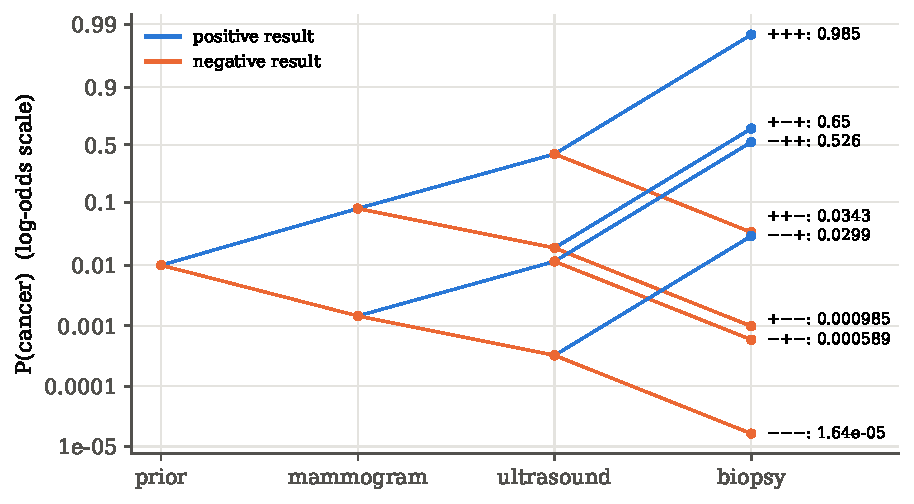
\includegraphics[width=0.86\linewidth]{figures/ch05/screening_paths.pdf}
\caption{The probability of cancer after each test, for every sequence of results,
on a log-odds axis, where each test moves the curve by the same step whatever came
before. A positive (blue) steps up by $\log_{10}\mathrm{LR}_+$, a negative (orange)
down by $\log_{10}\mathrm{LR}_-$; the end labels give the final probability for each
sequence. The biopsy's steps are much longer than the imaging tests', because its
likelihood ratios are much further from one.}
\label{5a:fig:screening-paths}
\end{figure}

\begin{figure}[htbp]
\centering
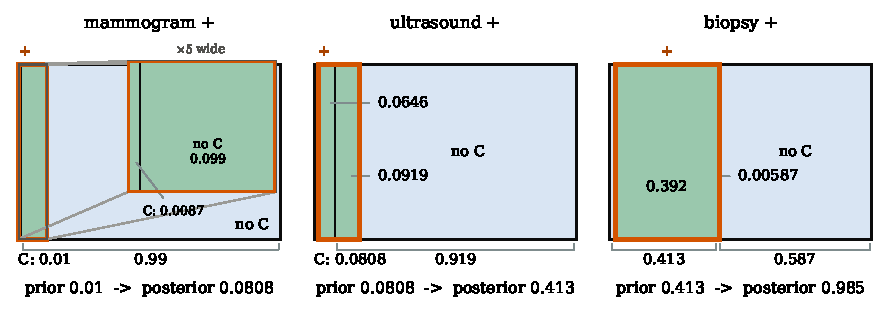
\includegraphics[width=\linewidth]{figures/ch05/screening_squares.pdf}
\caption{The sample space re-drawn before each test along the path $+,+,+$, in the
box picture of \cref{1a:fig:shrink}, with the function of \cref{5a:lst:area}. In each
panel the width of the cancer strip ($C$) is the current prior, and the positive
result is the box (orange outline): it covers the sensitivity's share of the $C$
strip and the false-alarm rate's share of the other, and the numbers are the areas
of its two pieces. Before the mammogram the cancer strip is $1\%$ of the width
(magnified in the inset); after it, the posterior $0.081$ becomes the width of the
strip for the ultrasound, and after the ultrasound, $0.41$ becomes the width for the
biopsy.}
\label{5a:fig:screening-squares}
\end{figure}

\paragraph{The assumption behind the multiplication.}
Multiplying the odds by each test's likelihood ratio assumes that the tests are
independent given her true state. For a healthy woman this says that a false alarm
on the mammogram makes a false alarm on the ultrasound neither more nor less likely.
That can fail: two imaging tests can be fooled by the same thing, since a benign
lump or very dense tissue may look suspicious to both. Model it as for the antibody
in the previous subsection. Say $5\%$ of healthy women carry such a feature and test
positive on both. The rest have independent false alarms at the rate $r=0.05/0.95$,
chosen so that each test alone still has false-positive rate $0.10$. Then three
numbers change:
$\Prob(M_+U_+\given C^c)=0.05+0.95\,r^2=\FiveAScrCorrHH$ instead of $0.01$; the
pair of positives has likelihood ratio
$0.87\times0.80/\FiveAScrCorrHH=\FiveAScrCorrLR$ instead of $8.7\times8.0=70$; and
her probability after two positive images is $\FiveAScrCorrPost$ (simulation
$\FiveAScrCorrMC$), not $\FiveAScrPP$. The second positive is worth less, because
much of what made the first one positive in a healthy woman repeats itself. The biopsy
examines the tissue itself, a different failure mode altogether, which is why it is
the test that settles the question.

\paragraph{Problem.}
In a younger screening population the prevalence is $0.5\%$. Test A has sensitivity
$0.90$ and specificity $0.92$; test B has sensitivity $0.85$ and specificity $0.95$.
(a) Assuming the tests are conditionally independent, find $\Prob(C\given A_+,B_+)$ and
$\Prob(C\given A_+,B_-)$. (b) How many independent positive results of test A are
needed for the probability of cancer to exceed $95\%$? (c) Now suppose that $3\%$ of
healthy women carry a benign feature that makes both A and B positive, while the
other healthy women have independent false positives at rates chosen so that each test
alone keeps its specificity. Redo (a), and say why the answers moved.

\paragraph{Solution.}
(a) The prior odds are $O_0=0.005/0.995=\FiveAPrbOzero$. The likelihood ratios are
$\mathrm{LR}_+^A=0.90/0.08=\FiveAPrbLAp$, $\mathrm{LR}_+^B=0.85/0.05=\FiveAPrbLBp$ and
$\mathrm{LR}_-^B=0.15/0.95=\FiveAPrbLBm$. Then
\begin{align*}
  O(C\given A_+,B_+)
  &\eqby{1}\mathrm{LR}_+^B\,\mathrm{LR}_+^A\,O_0
   =17.0\times11.25\times\FiveAPrbOzero=\FiveAPrbOAB,
  &\Prob(C\given A_+,B_+)&\eqby{2}\FiveAPrbAB,\\
  O(C\given A_+,B_-)
  &\eqby{3}\mathrm{LR}_-^B\,\mathrm{LR}_+^A\,O_0
   =\FiveAPrbOAb,
  &\Prob(C\given A_+,B_-)&=\FiveAPrbAb .
\end{align*}
\begin{explain}
  \item Two sequential updates in odds form; conditional independence lets each test
        enter through its own likelihood ratio.
  \item $p=O/(1+O)$.
  \item The same with the negative ratio of B.
\end{explain}
After a positive A alone the probability is $\FiveAPrbA$; a positive B brings it to
about one half, while a negative B brings it back to under $1\%$, still above the
prevalence of $0.5\%$.

(b) After $n$ independent positives of A the odds are $(\mathrm{LR}_+^A)^nO_0$, and
$95\%$ means odds of $19$:
\begin{align*}
  (\mathrm{LR}_+^A)^n\,O_0\ge19
  \;\relby{1}{\Longleftrightarrow}\;
  n\ge\frac{\ln(19/O_0)}{\ln\mathrm{LR}_+^A}
  =\frac{\ln3781}{\ln11.25}=3.40 .
\end{align*}
\begin{explain}
  \item Take logarithms; $\ln\mathrm{LR}_+^A>0$, so the inequality keeps its direction.
\end{explain}
So $n=\FiveAPrbN$: three positives give $\FiveAPrbNminus$, four give $\FiveAPrbNpost$.
This assumes that repeating test A on the same woman gives independent errors, which
for a repeated image of the same breast is exactly the assumption that part (c)
questions.

(c) With a fraction $g=0.03$ of healthy women carrying the feature, the other healthy
women must have false-positive rates $q_A=(0.08-g)/(1-g)=\FiveAPrbqA$ and
$q_B=(0.05-g)/(1-g)=\FiveAPrbqB$, so that each test alone is unchanged. For a healthy
woman,
\begin{align*}
  \Prob(A_+B_+\given C^c)
  &\eqby{1}g+(1-g)\,q_Aq_B=\FiveAPrbHAB,
  \qquad
  \Prob(A_+B_-\given C^c)
  \eqby{2}(1-g)\,q_A(1-q_B)=\FiveAPrbHAb,
\end{align*}
\begin{explain}
  \item Carriers are positive on both; the others are positive on both by two
        independent false alarms.
  \item A carrier is never negative on B, so only non-carriers contribute.
\end{explain}
while for a woman with cancer nothing changes,
$\Prob(A_+B_+\given C)=0.90\times0.85$ and $\Prob(A_+B_-\given C)=0.90\times0.15$.
The joint likelihood ratios replace the products of (a):
\begin{align*}
  \Prob(C\given A_+,B_+)
  &\eqby{1}\frac{O_0\cdot0.765/\FiveAPrbHAB}{1+O_0\cdot0.765/\FiveAPrbHAB}
   =\FiveAPrbABc,
  \qquad
  \Prob(C\given A_+,B_-)
  \eqby{2}\FiveAPrbAbc .
\end{align*}
\begin{explain}
  \item Odds form with the likelihood ratio of the \emph{pair} of results,
        $0.765/\FiveAPrbHAB=\FiveAPrbLRABc$, instead of $11.25\times17=\FiveAPrbLRABi$.
  \item The same with $0.135/\FiveAPrbHAb$.
\end{explain}
Both answers moved towards the prior. Two positives are now worth a factor
$\FiveAPrbLRABc$ rather than $\FiveAPrbLRABi$, because a healthy woman who is positive
on A is quite likely to be a carrier ($0.03/0.08$ of them), and a carrier is positive on
B for certain. The negative B is less reassuring for the same reason: among healthy
women positive on A, a negative B is now rarer, so it says less about health. The
script checks all four numbers by simulation, $\FiveAPrbMCAB$, $\FiveAPrbMCAb$,
$\FiveAPrbMCABc$ and $\FiveAPrbMCAbc$.
\section{The denominator: the sum over all paths}
\label{5a:sec:denominator}

The denominator $\Prob(E)$ of Bayes' theorem is the model's prediction for the
data. So far it has looked like bookkeeping: the number we divide by so that the
posteriors add up to one. In the odds form it cancelled altogether. But it is a
probability in its own right, and a meaningful one. Recall the trigger problem of
\cref{5a:sec:two-directions}, where $E$ was an isolated high-$p_T$ muon and three
trigger paths could have fired the event. There $\Prob(E)=0.235$. This says that,
\emph{before} we looked at the event, the model of the three paths predicted that
$23.5\%$ of recorded events would contain such a muon. Suppose a large sample of
events showed $60\%$. No reallocation of credibility among the three paths could
explain that. The trouble would lie in the list of paths or in the forward
probabilities, not in the priors. The denominator is also the one place in Bayes'
theorem that needs every hypothesis at once.

\subsection{Every path, and only paths}

The denominator is the marginalisation \eqref{5a:eq:marg}: the sum, over every
hypothesis, of the probability of reaching the observation along that hypothesis's
path (\cref{5a:fig:paths}),
\begin{equation}
  \Prob(E)=\sum_{i}\Prob(E\given H_i)\,\Prob(H_i)
  \quad\text{(discrete)},\qquad
  p(\data)=\int p(\data\given\theta)\,p(\theta)\,\dd\theta
  \quad\text{(continuous)} .
  \label{5a:eq:evidence}
\end{equation}
In the square of \cref{5a:sec:shrink} it is the total surviving area. It does not
depend on which hypothesis we are asking about. It depends only on the observation
and on the whole list of hypotheses with their priors. Two names are in use: the \newterm{evidence}, and the \newterm{marginal
likelihood}, because it is the likelihood averaged over the hypotheses with the prior
as the weight \srcref{Kruschke}{\S5.2, (5.8)--(5.9)}. Wasserman calls its continuous version $c_n=\int\Like_n(\theta)f(\theta)\,\dd\theta$ the
\newterm{normalizing constant} and notes that it can be dropped and recovered later
\mainref{p.~177, (11.3)}.

\begin{figure}[htbp]
\centering
\begin{tikzpicture}[
  font=\small,
  lvl/.style={draw=accent,rounded corners=2pt,fill=ideabg,minimum width=14mm,
              minimum height=6mm,align=center},
  leafE/.style={draw=formblue,thick,fill=formblue!12,rounded corners=2pt,
                minimum width=16mm,minimum height=6mm,align=center},
  path/.style={formblue,thick}]
  \node[lvl] (root) at (0,0) {event};
  \node[lvl] (mu)  at (-4.0,-1.6) {$H_\mu$};
  \node[lvl] (cal) at ( 0.0,-1.6) {$H_{\rm cal}$};
  \node[lvl] (trk) at ( 4.0,-1.6) {$H_{\rm trk}$};
  \draw[path] (root) -- (mu);
  \draw[path] (root) -- (cal);
  \draw[path] (root) -- (trk);
  \node[leafE] (mE) at (-4.0,-3.2) {$E$};
  \node[leafE] (cE) at ( 0.0,-3.2) {$E$};
  \node[leafE] (tE) at ( 4.0,-3.2) {$E$};
  \draw[path] (mu) -- (mE);
  \draw[path] (cal) -- (cE);
  \draw[path] (trk) -- (tE);
  \node[font=\footnotesize,anchor=west] at (-3.7,-2.4) {$0.25\times0.70$};
  \node[font=\footnotesize,anchor=west] at (0.3,-2.4) {$0.60\times0.05$};
  \node[font=\footnotesize,anchor=west] at (4.3,-2.4) {$0.15\times0.20$};
  \node[draw=formblue,thick,fill=formblue!8,rounded corners=2pt,align=center]
    (sum) at (0,-4.9) {$\Prob(E)=0.175+0.030+0.030=0.235$};
  \draw[path] (mE.south) -- (sum.north west);
  \draw[path] (cE.south) -- (sum.north);
  \draw[path] (tE.south) -- (sum.north east);
\end{tikzpicture}
\caption{The denominator of Bayes' theorem as the sum over paths. Each hypothesis
contributes one path from the root to the observed leaf $E$, with probability equal to
the product of its two branch probabilities (written beside the path). The evidence
collects all of them. A hypothesis missing from the tree is a path missing from the
sum.}
\label{5a:fig:paths}
\end{figure}

\subsection{The denominator is a prediction}

Now read \eqref{5a:eq:evidence} as a function of the data rather than as one number.
Before the data are taken, ask: how probable is each possible observation $E$? The
answer, $\Prob(E)$ for every $E$, is the model's forecast of what we are going to
see, averaged over our uncertainty about which hypothesis is true. It is called the \newterm{prior predictive distribution}
\srcref{Lambert}{\S6.3.4}. Unlike the likelihood, it is a genuine probability
distribution over the data: summed over all possible observations it gives one,
because $\sum_E\Prob(E\given H_i)=1$ for each $i$ and the priors sum to one.

\paragraph{Example: what did we expect from ten tosses?}
Take the grid of $101$ coin biases of \cref{5a:sec:sequential} with a flat prior, and
ask for the probability of $z$ heads in $N=10$ tosses before any toss is made. In the
continuum limit of the grid, the flat prior density is $p(\theta)=1$ on $[0,1]$, and
\begin{align}
  \Prob(z)
  &\eqby{1}\int_0^1\binom{N}{z}\theta^z(1-\theta)^{N-z}\,\dd\theta
   \eqby{2}\binom{N}{z}\frac{z!\,(N-z)!}{(N+1)!}
   \eqby{3}\frac{N!}{z!\,(N-z)!}\cdot\frac{z!\,(N-z)!}{(N+1)!}
   =\frac{1}{N+1} .
  \label{5a:eq:prior-pred}
\end{align}
\begin{explain}
  \item The evidence \eqref{5a:eq:evidence} with the binomial likelihood and the flat
        prior.
  \item The Beta integral $\int_0^1\theta^a(1-\theta)^b\,\dd\theta=a!\,b!/(a+b+1)!$ for
        integers $a,b\ge0$; it follows by integrating by parts $b$ times.
  \item Write out the binomial coefficient; the factorials cancel.
\end{explain}
Every number of heads from $0$ to $10$ was equally expected, with probability
$\frac{1}{11}=0.091$. The $101$-point grid gives $\FiveAEvFlat$ for $z=9$, the small
difference being the grid's approximation of the integral. A prior concentrated on
fair coins predicts something quite different (\cref{5a:fig:prior-pred}). If we are
certain that the coin is fair, $\Prob(z=9)=\binom{10}{9}2^{-10}=\FiveAEvFair$. The
triangular prior sits in between, $\FiveAEvTri$. Each prior predictive sums to one over
$z=0,\dots,10$, as the script confirms.

\begin{figure}[htbp]
\centering
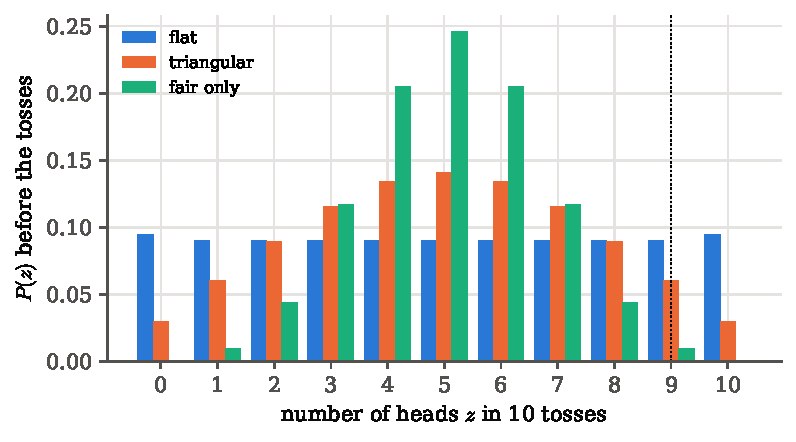
\includegraphics[width=0.8\linewidth]{figures/ch05/prior_predictive.pdf}
\caption{The denominator of Bayes' theorem as a forecast. For each of three beliefs
about the coin, the bars give the probability of each number of heads in ten tosses,
computed before any toss as a sum over all candidate biases. The flat prior spreads its
forecast evenly; ``the coin is fair'' concentrates it near five heads. The dotted line
marks the observed nine heads.}
\label{5a:fig:prior-pred}
\end{figure}

The whole computation is one matrix product:

\pyfile[firstline=33,lastline=35,firstnumber=33]{code/ch05/07_evidence.py}{The prior
predictive as a sum over paths}

Line 34 builds the table of \cref{5a:sec:two-directions}: one row per possible
observation $z$, one column per hypothesis $\theta_j$, entries $\Prob(z\given\theta_j)$.
Line 35 multiplies it by the vector of priors, which for each row is the sum over the
paths $\theta_j$ of likelihood times prior.

Now nine heads have been observed. Which model predicted that better? The
flat-prior model had given this outcome probability $\FiveAEvFlat$, the fair-coin
model only $\FiveAEvFair$. So the flat model predicted the observation
$\FiveAEvRatio$ times better. A ratio of two evidences is a likelihood ratio in which
each ``hypothesis'' is a whole model together with its prior. By \eqref{5a:eq:odds}
it multiplies the prior odds of one model against the other. This ratio, the
\emph{Bayes factor}, is the tool for comparing models, and comparing models is the
one job for which the denominator cannot be skipped.

\subsection{A missing path distorts every posterior}

Because the denominator sums over the hypotheses we listed, it silently assumes that
the list is complete. If the truth is not on the list, Bayes' theorem still returns
posteriors that sum to one, now shared among the wrong candidates. Kruschke's example
is the wet pavement caused by something nobody listed \srcref{Kruschke}{\S2.2}.

\paragraph{Example: forgetting the background.}
In the gamma-ray example of \cref{5a:sec:reallocation}, the soft photon at
$(-3^\circ,2^\circ)$ had source probabilities $\FiveAGrbMbG$ (burst), $\FiveAGrbMbB$
(blazar) and $\FiveAGrbMbD$ (diffuse background). Suppose we forget the diffuse
background and keep only the two point sources. The denominator loses the largest of
its three paths, and the same photon now gets $\FiveAGrbForgotG$ for the burst and
$\FiveAGrbForgotB$ for the blazar. Nothing in the output warns us: the posteriors still
sum to one. The warning is in the denominator itself. Without the background, the model
predicts that almost no photons arrive far from the two point sources, so the evidence
of a map full of such photons is tiny compared with that of the model with the
background. Comparing evidences, or checking whether the most credible hypotheses
actually reproduce the data \srcref{Kruschke}{\S2.2}, is how a missing path is found.

\begin{pitfall}[A small evidence is not by itself a refutation]
Every particular data set has a small probability: any one sequence of ten tosses has
probability $2^{-10}\approx0.001$ under a fair coin. The value of $\Prob(E)$ alone says
little. It becomes informative when compared, either with the evidence of another
model for the same data, or with the spread of $\Prob(E)$ over the data sets the model
itself would typically produce.
\end{pitfall}

\subsection{Why the denominator is the hard part}

The denominator is hard because it needs every hypothesis at once, and in many
dimensions there are far too many. For a handful of hypotheses the sum
\eqref{5a:eq:evidence} is trivial. For a continuous parameter it is an integral,
which a grid approximates by a sum, as in the $101$-point coin grid. For $D$
parameters a grid with $n$ points per axis has $n^D$ points. With $n=1000$ and
$D=6$, the number of parameters of the standard cosmological model, that is
$10^{18}$ evaluations of the likelihood \srcref{Kruschke}{\S5.4},
\srcref{Lambert}{\S6.4}.

There are two ways out. The first is to choose priors that match the form of the
likelihood, so that the integral can be done by hand; these \emph{conjugate}
priors give posteriors of a known shape. The second is to notice that estimating
parameters never needs the denominator at all. It cancels in every ratio of
posteriors, exactly as it cancelled in the odds \eqref{5a:eq:odds}. A method that
only ever compares the posterior at two points,
$p(\theta'\given\data)/p(\theta\given\data)=p(\data\given\theta')p(\theta')/p(\data\given\theta)p(\theta)$,
can explore the posterior without knowing its normalisation. That is the idea behind
Markov chain Monte Carlo (\cref{ch:09}) \srcref{Lambert}{\S6.5}. Only when models
themselves are compared must the evidence be computed, and that needs its own methods.

The trigger paths, the medical test, Monty's door, the urns and the ball sizes
were all solved in the same way, and the way is worth making a habit: put the
question into words before touching a symbol. First ask: which hypotheses could
have produced what we observed? With that list settled, ask: how probable would
the observation have been if each of them were true? These two answers sort the
whole problem. The first answer says what the posterior is a distribution over,
and so fixes the list of paths that the denominator sums over. The second answer
is the likelihood: it fixes the height of each bar in the square.

\begin{recap}
\begin{itemize}[itemsep=2pt,leftmargin=1.2em]
  \item Prediction reads $\Prob(E\given H)$, inference wants $\Prob(H\given E)$. Both
        come from one joint distribution: a column of the joint table for prediction,
        the observed row for inference.
  \item Bayes' theorem is the product rule applied in both orders. Observing $E$
        shrinks the sample space to $E$; each hypothesis is re-measured by its share of
        the surviving region.
  \item In the unit square: priors are widths, likelihoods are heights, joint
        probabilities are areas, the evidence is the surviving area, and the posterior
        is one surviving rectangle over all of them.
  \item Base rates matter: evidence covering most of a thin strip (medical test,
        trigger purity, rare signal) can lose to evidence covering a small share of
        a wide strip.
  \item Inference is reallocation of credibility: a zero likelihood eliminates, a zero
        prior can never be revived, noisy data only nudge.
  \item Posterior odds $=$ likelihood ratio $\times$ prior odds. The likelihood ratio is
        all the evidence says about two hypotheses; in logarithms, independent evidence
        adds (decibels, log-odds random walk with drift equal to a Kullback--Leibler
        divergence).
  \item Condition on exactly what was observed: ``score $=0.8$'' and ``score $>0.8$'' are
        different evidence.
  \item Sequential updating: the posterior becomes the prior; the order of the data
        does not matter; multiplying likelihoods requires independence given the
        hypothesis.
  \item The denominator is the sum over all paths: the normaliser, the prior
        predictive forecast of the data, and the quantity that compares models. It
        needs the complete list of hypotheses and is hard to compute in many
        dimensions, which is why parameter estimation works with ratios of posteriors.
\end{itemize}
\end{recap}

\providecommand{\FiveBGd}{}\renewcommand{\FiveBGd}{0.6041}
\providecommand{\FiveBGsig}{}\renewcommand{\FiveBGsig}{0.1}
\providecommand{\FiveBGtrue}{}\renewcommand{\FiveBGtrue}{0.8}
\providecommand{\FiveBGpeak}{}\renewcommand{\FiveBGpeak}{0.777}
\providecommand{\FiveBGsqrtd}{}\renewcommand{\FiveBGsqrtd}{0.7772}
\providecommand{\FiveBGmasspos}{}\renewcommand{\FiveBGmasspos}{0.5}
\providecommand{\FiveBGevid}{}\renewcommand{\FiveBGevid}{0.4336}
\providecommand{\FiveBTauN}{}\renewcommand{\FiveBTauN}{2000}
\providecommand{\FiveBTauRawMax}{}\renewcommand{\FiveBTauRawMax}{\infty}
\providecommand{\FiveBTauRawMaxPct}{}\renewcommand{\FiveBTauRawMaxPct}{0}
\providecommand{\FiveBTauLogLmax}{}\renewcommand{\FiveBTauLogLmax}{3149}
\providecommand{\FiveBTauMean}{}\renewcommand{\FiveBTauMean}{1.996}
\providecommand{\FiveBTauSd}{}\renewcommand{\FiveBTauSd}{0.007948}
\providecommand{\FiveBTauSigd}{}\renewcommand{\FiveBTauSigd}{0.05}
\providecommand{\FiveBBetaModeS}{}\renewcommand{\FiveBBetaModeS}{0.5321}
\providecommand{\FiveBBetaModeL}{}\renewcommand{\FiveBBetaModeL}{0.7965}
\providecommand{\FiveBBetaModeF}{}\renewcommand{\FiveBBetaModeF}{0.85}
\providecommand{\FiveBBetaHdiSlo}{}\renewcommand{\FiveBBetaHdiSlo}{0.466}
\providecommand{\FiveBBetaHdiShi}{}\renewcommand{\FiveBBetaHdiShi}{0.5975}
\providecommand{\FiveBBetaHdiLlo}{}\renewcommand{\FiveBBetaHdiLlo}{0.6629}
\providecommand{\FiveBBetaHdiLhi}{}\renewcommand{\FiveBBetaHdiLhi}{0.8966}
\providecommand{\FiveBBetaHdiFlo}{}\renewcommand{\FiveBBetaHdiFlo}{0.6599}
\providecommand{\FiveBBetaHdiFhi}{}\renewcommand{\FiveBBetaHdiFhi}{0.9591}
\providecommand{\FiveBBetaErr}{}\renewcommand{\FiveBBetaErr}{1.247\times10^{-11}}
\providecommand{\FiveBCountsSum}{}\renewcommand{\FiveBCountsSum}{28}
\providecommand{\FiveBCountsList}{}\renewcommand{\FiveBCountsList}{3, 5, 7, 4, 9}
\providecommand{\FiveBGamA}{}\renewcommand{\FiveBGamA}{31}
\providecommand{\FiveBGamB}{}\renewcommand{\FiveBGamB}{6}
\providecommand{\FiveBGamMean}{}\renewcommand{\FiveBGamMean}{5.167}
\providecommand{\FiveBGamSd}{}\renewcommand{\FiveBGamSd}{0.928}
\providecommand{\FiveBGamErr}{}\renewcommand{\FiveBGamErr}{1.018\times10^{-11}}
\providecommand{\FiveBGamMLE}{}\renewcommand{\FiveBGamMLE}{5.6}
\providecommand{\FiveBNxa}{}\renewcommand{\FiveBNxa}{10.2}
\providecommand{\FiveBNxb}{}\renewcommand{\FiveBNxb}{9.936}
\providecommand{\FiveBNxc}{}\renewcommand{\FiveBNxc}{10.07}
\providecommand{\FiveBNmPost}{}\renewcommand{\FiveBNmPost}{10.1}
\providecommand{\FiveBNsPost}{}\renewcommand{\FiveBNsPost}{0.4319}
\providecommand{\FiveBNmIvw}{}\renewcommand{\FiveBNmIvw}{10.15}
\providecommand{\FiveBNsIvw}{}\renewcommand{\FiveBNsIvw}{0.4364}
\providecommand{\FiveBNErr}{}\renewcommand{\FiveBNErr}{2.260\times10^{-14}}
\providecommand{\FiveBPred}{}\renewcommand{\FiveBPred}{0.4853}
\providecommand{\FiveBPlugin}{}\renewcommand{\FiveBPlugin}{0.5102}
\providecommand{\FiveBULzero}{}\renewcommand{\FiveBULzero}{2.996}
\providecommand{\FiveBULone}{}\renewcommand{\FiveBULone}{4.744}
\providecommand{\FiveBULthree}{}\renewcommand{\FiveBULthree}{7.754}
\providecommand{\FiveBCmbModeTwo}{}\renewcommand{\FiveBCmbModeTwo}{0.7143}
\providecommand{\FiveBCmbMeanTwo}{}\renewcommand{\FiveBCmbMeanTwo}{1.667}
\providecommand{\FiveBCmbLoTwo}{}\renewcommand{\FiveBCmbLoTwo}{0.6303}
\providecommand{\FiveBCmbHiTwo}{}\renewcommand{\FiveBCmbHiTwo}{2.421}
\providecommand{\FiveBCmbLoFifty}{}\renewcommand{\FiveBCmbLoFifty}{0.8776}
\providecommand{\FiveBCmbHiFifty}{}\renewcommand{\FiveBCmbHiFifty}{1.162}
\providecommand{\FiveBCmbModeFifty}{}\renewcommand{\FiveBCmbModeFifty}{0.9806}
\providecommand{\FiveBGwAhat}{}\renewcommand{\FiveBGwAhat}{1.06}
\providecommand{\FiveBGwAsd}{}\renewcommand{\FiveBGwAsd}{0.1}
\providecommand{\FiveBGwSpread}{}\renewcommand{\FiveBGwSpread}{0.1008}
\providecommand{\FiveBGwHH}{}\renewcommand{\FiveBGwHH}{100}
\providecommand{\FiveBSumAboveMode}{}\renewcommand{\FiveBSumAboveMode}{78}
\providecommand{\FiveBSumMean}{}\renewcommand{\FiveBSumMean}{1.667}
\providecommand{\FiveBSumMedian}{}\renewcommand{\FiveBSumMedian}{1.149}
\providecommand{\FiveBSumMode}{}\renewcommand{\FiveBSumMode}{0.7143}
\providecommand{\FiveBSumEtiLo}{}\renewcommand{\FiveBSumEtiLo}{0.3896}
\providecommand{\FiveBSumEtiHi}{}\renewcommand{\FiveBSumEtiHi}{6.015}
\providecommand{\FiveBSumHdiLo}{}\renewcommand{\FiveBSumHdiLo}{0.2294}
\providecommand{\FiveBSumHdiHi}{}\renewcommand{\FiveBSumHdiHi}{4.389}
\providecommand{\FiveBSumHdiSLo}{}\renewcommand{\FiveBSumHdiSLo}{0.2275}
\providecommand{\FiveBSumHdiSHi}{}\renewcommand{\FiveBSumHdiSHi}{4.356}
\providecommand{\FiveBSumHdiYLo}{}\renewcommand{\FiveBSumHdiYLo}{0.348}
\providecommand{\FiveBSumHdiYHi}{}\renewcommand{\FiveBSumHdiYHi}{5.054}
\providecommand{\FiveBSumWater}{}\renewcommand{\FiveBSumWater}{0.02375}
\providecommand{\FiveBBiLoA}{}\renewcommand{\FiveBBiLoA}{-0.8394}
\providecommand{\FiveBBiHiA}{}\renewcommand{\FiveBBiHiA}{-0.7096}
\providecommand{\FiveBBiLoB}{}\renewcommand{\FiveBBiLoB}{0.7096}
\providecommand{\FiveBBiHiB}{}\renewcommand{\FiveBBiHiB}{0.8394}
\providecommand{\FiveBBiMean}{}\renewcommand{\FiveBBiMean}{0.000}
\providecommand{\FiveBLapHa}{}\renewcommand{\FiveBLapHa}{0.2812}
\providecommand{\FiveBLapSa}{}\renewcommand{\FiveBLapSa}{0.07948}
\providecommand{\FiveBLapMeanA}{}\renewcommand{\FiveBLapMeanA}{0.2941}
\providecommand{\FiveBLapSdA}{}\renewcommand{\FiveBLapSdA}{0.07702}
\providecommand{\FiveBLapHb}{}\renewcommand{\FiveBLapHb}{0.1}
\providecommand{\FiveBLapSb}{}\renewcommand{\FiveBLapSb}{0.09487}
\providecommand{\FiveBLapNegB}{}\renewcommand{\FiveBLapNegB}{0.1459}
\providecommand{\FiveBLapMeanB}{}\renewcommand{\FiveBLapMeanB}{0.1667}
\providecommand{\FiveBLapSdB}{}\renewcommand{\FiveBLapSdB}{0.1034}
\providecommand{\FiveBLhModeFive}{}\renewcommand{\FiveBLhModeFive}{1.096}
\providecommand{\FiveBLhSdFive}{}\renewcommand{\FiveBLhSdFive}{0.06506}
\providecommand{\FiveBLhXbarFive}{}\renewcommand{\FiveBLhXbarFive}{1.197}
\providecommand{\FiveBLhModeSix}{}\renewcommand{\FiveBLhModeSix}{1.34}
\providecommand{\FiveBLhSdSix}{}\renewcommand{\FiveBLhSdSix}{0.2039}
\providecommand{\FiveBLhLapSix}{}\renewcommand{\FiveBLhLapSix}{0.2026}
\providecommand{\FiveBLhXbarSix}{}\renewcommand{\FiveBLhXbarSix}{3.578}
\providecommand{\FiveBLhSqrtTwoN}{}\renewcommand{\FiveBLhSqrtTwoN}{0.0625}
\providecommand{\FiveBMaRhoWide}{}\renewcommand{\FiveBMaRhoWide}{-0.6688}
\providecommand{\FiveBMaRhoNarrow}{}\renewcommand{\FiveBMaRhoNarrow}{-0.9331}
\providecommand{\FiveBMaSigWide}{}\renewcommand{\FiveBMaSigWide}{0.2075}
\providecommand{\FiveBMaSigCondWide}{}\renewcommand{\FiveBMaSigCondWide}{0.1538}
\providecommand{\FiveBMaSigNarrow}{}\renewcommand{\FiveBMaSigNarrow}{0.4197}
\providecommand{\FiveBMaSigCondNarrow}{}\renewcommand{\FiveBMaSigCondNarrow}{0.1517}
\providecommand{\FiveBVolMargMode}{}\renewcommand{\FiveBVolMargMode}{0}
\providecommand{\FiveBVolProfMode}{}\renewcommand{\FiveBVolProfMode}{0.83}
\providecommand{\FiveBVolMargMean}{}\renewcommand{\FiveBVolMargMean}{0.5447}
\providecommand{\FiveBVolPsmallMarg}{}\renewcommand{\FiveBVolPsmallMarg}{0.5375}
\providecommand{\FiveBVolPsmallProf}{}\renewcommand{\FiveBVolPsmallProf}{0.2077}
\providecommand{\FiveBVolAtrue}{}\renewcommand{\FiveBVolAtrue}{1.2}
\providecommand{\FiveBVolLoopR}{}\renewcommand{\FiveBVolLoopR}{500}
\providecommand{\FiveBVolLoopPsmallMarg}{}\renewcommand{\FiveBVolLoopPsmallMarg}{0.20}
\providecommand{\FiveBVolLoopPsmallProf}{}\renewcommand{\FiveBVolLoopPsmallProf}{0.07}
\providecommand{\FiveBVolLoopErr}{}\renewcommand{\FiveBVolLoopErr}{0.01}
\providecommand{\FiveBVolLoopModeZero}{}\renewcommand{\FiveBVolLoopModeZero}{50}
\providecommand{\FiveBPrFracCentral}{}\renewcommand{\FiveBPrFracCentral}{0.763}
\providecommand{\FiveBPrFlatTop}{}\renewcommand{\FiveBPrFlatTop}{0.9001}
\providecommand{\FiveBPrFlatBottom}{}\renewcommand{\FiveBPrFlatBottom}{9.001\times10^{-4}}
\providecommand{\FiveBPrLogDecade}{}\renewcommand{\FiveBPrLogDecade}{0.25}
\providecommand{\FiveBPrFlatMeanTen}{}\renewcommand{\FiveBPrFlatMeanTen}{0.1667}
\providecommand{\FiveBPrFlatUpTen}{}\renewcommand{\FiveBPrFlatUpTen}{0.3644}
\providecommand{\FiveBPrFlatMeanThou}{}\renewcommand{\FiveBPrFlatMeanThou}{0.1008}
\providecommand{\FiveBPrFlatUpThou}{}\renewcommand{\FiveBPrFlatUpThou}{0.1169}
\providecommand{\FiveBPrJefMeanTen}{}\renewcommand{\FiveBPrJefMeanTen}{0.1364}
\providecommand{\FiveBPrJefUpTen}{}\renewcommand{\FiveBPrJefUpTen}{0.3306}
\providecommand{\FiveBPrJefMeanThou}{}\renewcommand{\FiveBPrJefMeanThou}{0.1004}
\providecommand{\FiveBPrJefUpThou}{}\renewcommand{\FiveBPrJefUpThou}{0.1165}
\providecommand{\FiveBPrHalMeanTen}{}\renewcommand{\FiveBPrHalMeanTen}{0.1}
\providecommand{\FiveBPrHalUpTen}{}\renewcommand{\FiveBPrHalUpTen}{0.2831}
\providecommand{\FiveBPrHalMeanThou}{}\renewcommand{\FiveBPrHalMeanThou}{0.1}
\providecommand{\FiveBPrHalUpThou}{}\renewcommand{\FiveBPrHalUpThou}{0.116}
\providecommand{\FiveBBvmGapTen}{}\renewcommand{\FiveBBvmGapTen}{1.452}
\providecommand{\FiveBBvmGapThou}{}\renewcommand{\FiveBBvmGapThou}{2.949}
\providecommand{\FiveBBvmGapLast}{}\renewcommand{\FiveBBvmGapLast}{0.3407}
\providecommand{\FiveBBvmGapPeak}{}\renewcommand{\FiveBBvmGapPeak}{5.885}
\providecommand{\FiveBBvmNpeak}{}\renewcommand{\FiveBBvmNpeak}{122}
\providecommand{\FiveBBvmNone}{}\renewcommand{\FiveBBvmNone}{12999}
\providecommand{\FiveBBvmNtot}{}\renewcommand{\FiveBBvmNtot}{5068}
\providecommand{\FiveBChainFlatA}{}\renewcommand{\FiveBChainFlatA}{0.3147}
\providecommand{\FiveBChainFlatB}{}\renewcommand{\FiveBChainFlatB}{0.3182}
\providecommand{\FiveBChainStrA}{}\renewcommand{\FiveBChainStrA}{0.7172}
\providecommand{\FiveBChainStrB}{}\renewcommand{\FiveBChainStrB}{0.716}
\providecommand{\FiveBChainExactFlat}{}\renewcommand{\FiveBChainExactFlat}{0.3182}
\providecommand{\FiveBChainExactStr}{}\renewcommand{\FiveBChainExactStr}{0.7167}
\providecommand{\FiveBSaTwoHeads}{}\renewcommand{\FiveBSaTwoHeads}{0.4839}
\providecommand{\FiveBSaTwoHeadsExact}{}\renewcommand{\FiveBSaTwoHeadsExact}{0.4853}
\providecommand{\FiveBSaPredLo}{}\renewcommand{\FiveBSaPredLo}{0}
\providecommand{\FiveBSaPredHi}{}\renewcommand{\FiveBSaPredHi}{4}
\providecommand{\FiveBSaPlugHi}{}\renewcommand{\FiveBSaPlugHi}{2}
\providecommand{\FiveBSaPredZero}{}\renewcommand{\FiveBSaPredZero}{0.2612}
\providecommand{\FiveBSaPlugZero}{}\renewcommand{\FiveBSaPlugZero}{0.3487}
\providecommand{\FiveBSaPpos}{}\renewcommand{\FiveBSaPpos}{0.9877}
\providecommand{\FiveBSaTauLo}{}\renewcommand{\FiveBSaTauLo}{0.03117}
\providecommand{\FiveBSaTauHi}{}\renewcommand{\FiveBSaTauHi}{0.4355}
\providecommand{\FiveBSaB}{}\renewcommand{\FiveBSaB}{200000}
 
\section{From a list of hypotheses to a continuous parameter}
\label{5b:sec:continuous}

A theorist hands us a formula. If a parameter $\lambda$ of nature has a certain value,
an instrument should read $\mu(\lambda)$. The parameter could be the mass of a
particle, a coupling, a lifetime or the matter density of the universe. The instrument
is not perfect, so what it actually reads is the prediction plus some noise. We take
one reading, $d$. Which values of $\lambda$ could have produced it, and how much
credibility should each value get?

We answer it in the same order as the Monty Hall problem (\cref{5a:fig:monty}).
\emph{The event.} What we observed is ``the instrument showed $d$''.
\emph{The question.} What made it show that value? The possible explanations are the
possible values of $\lambda$, each one a possible state of nature.
\emph{Each candidate in turn.} For each value of $\lambda$ we ask how probable the
reading $d$ was if that value were the truth. The prediction would then have been
$\mu(\lambda)$, so the question is how likely the noise was to push $\mu(\lambda)$ to
exactly the $d$ we saw.
\emph{Only then the priors, and the normalisation.} We multiply by the prior weight of
each value and divide by the total.

This is the question ``which urn did the ball come from?'' or ``is this event signal
or background?'' with one change. There the candidate explanations formed a short
list, $H_1,H_2,\dots$. Here every real number in some range is a candidate. Bayes'
theorem still holds, but three things need care. A probability spread over a continuum
is a density. The sum over paths in the denominator becomes an integral. And a computer
can evaluate the density only at finitely many points.

\subsection{The tree, continuous in spirit}

Write the reading as prediction plus noise,
\begin{equation}
  d=\mu(\lambda)+\epsilon,\qquad \epsilon\sim\Normal(0,\sigma^2),
  \label{5b:eq:model}
\end{equation}
where $\sigma$ is the known size of the noise. The forward question, prediction, asks:
if nature chose $\lambda$, what readings would we see, and how often? Its answer is a
Gaussian centred on the prediction,
\begin{equation}
  p(d\given\lambda)=\frac{1}{\sqrt{2\pi\sigma^2}}
  \exp\!\left[-\frac{\bigl(d-\mu(\lambda)\bigr)^2}{2\sigma^2}\right].
  \label{5b:eq:gauss-like}
\end{equation}
Held at the reading we have and read as a function of $\lambda$, it is the
\newterm{likelihood} $\Like(\lambda)$, which scores each candidate by the
probability of the noise, $d-\mu(\lambda)$, it would have needed
(\cref{3b:sec:likelihood}).

The inference question runs the other way, and its picture is a probability tree with
one branch per candidate value (\cref{5b:fig:tree}). The first split chooses $\lambda$
with prior weight $p(\lambda)$. The second step produces the reading, with probability
$p(d\given\lambda)$ along each branch. Every branch can reach the same leaf $d$,
because Gaussian noise can turn any prediction into any reading, only with very
different probabilities. With infinitely many branches the tree cannot be drawn
literally, but it can be drawn in spirit: pick three candidates $\lambda_1,\lambda_2,
\lambda_3$ and remember that there is one branch for every value in between.

\begin{figure}[htbp]
\centering
\begin{tikzpicture}[x=1cm,y=1cm]
  \draw[faint,->] (-4.2,3.0) -- (4.4,3.0) node[right,lbl,black] {$\lambda$};
  \draw[form,domain=-4:4,samples=80] plot (\x,{3.0+0.9*exp(-(\x+0.6)^2/5)});
  \node[lbl,formblue,anchor=east] at (-4.25,3.55) {$p(\lambda)$};
  \node[lbl,draw,rounded corners,fill=white] (root) at (0,4.6) {possible values of $\lambda$};
  \foreach \xx/\nm in {-2.8/1,0/2,2.8/3}{
    \pgfmathsetmacro{\yy}{3.0+0.9*exp(-(\xx+0.6)^2/5)}
    \fill[formblue] (\xx,\yy) circle (1.4pt);
    \draw[->,thick,black!70] (root.south) -- (\xx,2.3);
    \node[lbl,anchor=east] at (\xx-0.1,2.05) {$\lambda_\nm$};
    \draw[->,thick,black!70] (\xx,1.85) -- (\xx,0.75);
    \node[lbl] at (\xx,0.45) {$d$};
    \node[lbl] at (\xx,0.0) {$p(d\given\lambda_\nm)$};
  }
  \foreach \xx in {-3.6,-2.2,-1.6,-1.0,-0.5,0.5,1.0,1.6,2.2,3.6}{
    \draw[faint,black!25] (root.south) -- (\xx,2.3);
  }
  \draw[faint,->] (-4.2,-1.4) -- (4.4,-1.4) node[right,lbl,black] {$\lambda$};
  \draw[thick,tangentgreen,domain=-4:4,samples=80] plot (\x,{-1.4+0.9*exp(-(\x-0.9)^2/1.2)});
  \node[lbl,tangentgreen,anchor=east] at (-4.25,-0.8) {$p(d\given\lambda)$};
\end{tikzpicture}
\caption{The probability tree for a continuous parameter, drawn in spirit. The top
curve is the prior density, the weight with which each branch is chosen. Three branches
are drawn in full and the faint fan stands for the continuum of branches between them.
Every branch can end at the same observed reading $d$, each with its own probability.
The bottom curve collects those probabilities as a function of $\lambda$: the
likelihood.}
\label{5b:fig:tree}
\end{figure}

\begin{keyidea}[Parameter estimation is inference with a continuum of explanations]
Every candidate value of the parameter $\lambda$ is one possible explanation of
the data. The reading $d$ is the event that actually happened. The likelihood
$\Like(\lambda)=p(d\given\lambda)$ measures, value by value, how easily that
$\lambda$ could have produced the event.
\end{keyidea}

\subsection{From a sum over branches to a density}

What does Bayes' theorem become when the hypotheses form a continuum? We reduce the
question to the case we already know, a finite list. Chop the $\lambda$ axis into cells
of small width $\Delta\lambda$, centred on the points $\lambda_j$, and call
``$\lambda$ lies in cell $j$'' hypothesis $H_j$. Exactly one cell contains the true
value, so these hypotheses are a partition and the discrete theorem applies to them.
The prior probability of cell $j$ is $\Prob(H_j)\approx p(\lambda_j)\,\Delta\lambda$,
because a density times a small width is a probability. Then
\begin{align}
  \frac{\Prob(H_j\given d)}{\Delta\lambda}
  &\eqby{1}\frac{1}{\Delta\lambda}\,
     \frac{p(d\given\lambda_j)\,p(\lambda_j)\,\Delta\lambda}
          {\sum_k p(d\given\lambda_k)\,p(\lambda_k)\,\Delta\lambda}
   \nonumber\\
  &\eqby{2}\frac{p(d\given\lambda_j)\,p(\lambda_j)}
          {\sum_k p(d\given\lambda_k)\,p(\lambda_k)\,\Delta\lambda}
   \nonumber\\
  &\xrightarrow{\ \Delta\lambda\to0\ }
   \frac{p(d\given\lambda_j)\,p(\lambda_j)}{\int p(d\given\lambda)\,p(\lambda)\,\dd\lambda} .
  \label{5b:eq:bayes-cont}
\end{align}
\begin{explain}
  \item Discrete Bayes' theorem for the cells, with the prior probability of each cell
        written as density times width.
  \item The $\Delta\lambda$ in the numerator cancels the $1/\Delta\lambda$ in front.
        The one in the denominator stays inside the sum.
\end{explain}
Now let the cells shrink. In the denominator each term is multiplied by its width, so
the sum is a Riemann sum and becomes an integral. On the left, the probability of a cell
divided by its width becomes a probability per unit $\lambda$: the
\newterm{posterior density} $p(\lambda\given d)$. So the continuous theorem is
\mainref{p.~177, (11.1)}
\begin{equation}
  p(\lambda\given d)=\frac{p(d\given\lambda)\,p(\lambda)}{p(d)},\qquad
  p(d)=\int p(d\given\lambda)\,p(\lambda)\,\dd\lambda .
  \label{5b:eq:bayes}
\end{equation}
The denominator $p(d)$ is the old sum over every path to the observation, now an
integral over every branch of the tree in \cref{5b:fig:tree}. It does not depend on
$\lambda$, so the shape of the posterior is set by the numerator alone
\mainref{p.~177, (11.2)--(11.3)}:
\begin{equation}
  p(\lambda\given d)\;\propto\;\Like(\lambda)\,p(\lambda),
  \label{5b:eq:prop}
\end{equation}
``posterior is proportional to likelihood times prior''. The constant is recovered at
the end by demanding that $\int p(\lambda\given d)\,\dd\lambda=1$.

\begin{workdef}[posterior density]
The \newterm{posterior density} of a continuous parameter $\lambda$ given data $d$ is
$p(\lambda\given d)=\Like(\lambda)\,p(\lambda)/p(d)$, where $\Like(\lambda)=p(d\given
\lambda)$ is the likelihood \unpack{the probability density of the data actually
observed, read as a function of $\lambda$}, $p(\lambda)$ is the prior density
\unpack{credibility per unit $\lambda$ before the data}, and $p(d)$ is the evidence
\unpack{the same product integrated over all $\lambda$. It makes the posterior
integrate to one}. \emph{Operationally:} evaluate $\Like(\lambda)p(\lambda)$ at every
$\lambda$ you care about, and divide by its integral. The probability that $\lambda$
lies between $a$ and $b$ is $\int_a^bp(\lambda\given d)\,\dd\lambda$.
\end{workdef}

A density is not itself a probability. Its value at a point, say $p(\lambda\given d)=
3$, means ``probability $3\,\Delta\lambda$ for a small cell of width $\Delta\lambda$
around this point'', and it carries units of one over the units of $\lambda$. Only areas
under the curve are probabilities. This matters as soon as we change variables
(\cref{5b:sec:priors}): the height of a density changes when we stretch the axis,
while the probabilities of corresponding intervals do not.

\paragraph{Example: a linear prediction and a flat prior.}
Let $\mu(\lambda)=\lambda$, so the instrument reads the parameter itself plus noise,
and take a prior that is constant, $p(\lambda)=1/(\lambda_{\max}-\lambda_{\min})$, over
a range much wider than $\sigma$ and containing $d$. Then
\begin{align*}
  p(\lambda\given d)
  &\eqby{1}\frac{\Like(\lambda)\,p(\lambda)}{\int\Like(\lambda')\,p(\lambda')\,\dd\lambda'}
   \eqby{2}\frac{e^{-(d-\lambda)^2/2\sigma^2}}{\int_{\lambda_{\min}}^{\lambda_{\max}}
       e^{-(d-\lambda')^2/2\sigma^2}\dd\lambda'}
   \eqby{3}\frac{1}{\sqrt{2\pi\sigma^2}}\,e^{-(\lambda-d)^2/2\sigma^2}.
\end{align*}
\begin{explain}
  \item Bayes' theorem \eqref{5b:eq:bayes}.
  \item The flat prior is the same constant in numerator and denominator and cancels,
        and so does the factor $1/\sqrt{2\pi\sigma^2}$ of the likelihood.
  \item The range is many $\sigma$ wide around $d$, so the integral is, to excellent
        accuracy, the full Gaussian integral $\int_{-\infty}^\infty e^{-u^2/2\sigma^2}
        \dd u=\sqrt{2\pi\sigma^2}$.
\end{explain}
The posterior is a Gaussian in $\lambda$, centred on the reading $d$, with width equal
to the noise size $\sigma$. Values of $\lambda$ whose prediction lies close to the
reading get the most credibility. The formula looks like the likelihood with $d$ and
$\lambda$ swapped, and here it is exactly that. But this is a coincidence of the linear
prediction $\mu(\lambda)=\lambda$, as the next example shows.

\paragraph{Example: a rate that depends on the square of a coupling.}
Many rates in particle physics are proportional to the square of a coupling $g$: a
decay width, a cross-section, an oscillation probability. Take $\mu(g)=g^2$ in suitable
units, with noise $\sigma=\FiveBGsig$, and suppose the true coupling is
$g=\FiveBGtrue$.
\emph{The event.} One simulated reading came out as $d=\FiveBGd$.
\emph{The question.} Which couplings could have produced it? A coupling $g$ predicts
the rate $g^2$, so the candidates that explain the reading well are those with $g^2$
close to $d$.
\emph{The candidates.} There are two groups of them, not one: $g$ near $+\sqrt d$ and
$g$ near $-\sqrt d$. The reason is that $g$ and $-g$ predict the same rate, so no
reading can tell them apart.
\emph{Only then the numbers.} With a flat prior on $g\in[-1.5,1.5]$,
\begin{equation*}
  p(g\given d)\propto\exp\!\left[-\frac{(d-g^2)^2}{2\sigma^2}\right].
\end{equation*}
This is largest where $g^2=d$, that is at the \emph{two} points $g=\pm\sqrt d=
\pm\FiveBGsqrtd$ (\cref{5b:fig:coupling}). The function is even in $g$, so exactly half
the posterior probability lies on each side: the computed mass at $g>0$ is
$\FiveBGmasspos$.
\emph{What it means.} The data say ``$|g|$ is about $\FiveBGsqrtd$'' and nothing about
the sign. The posterior reports this honestly with two peaks; a single ``best value
with an error bar'' could not. If theory tells us that $g>0$, that is prior
information. Put it in the prior, $p(g)=0$ for $g<0$, and the posterior becomes the
right-hand peak alone, renormalised.

\begin{figure}[htbp]
\centering
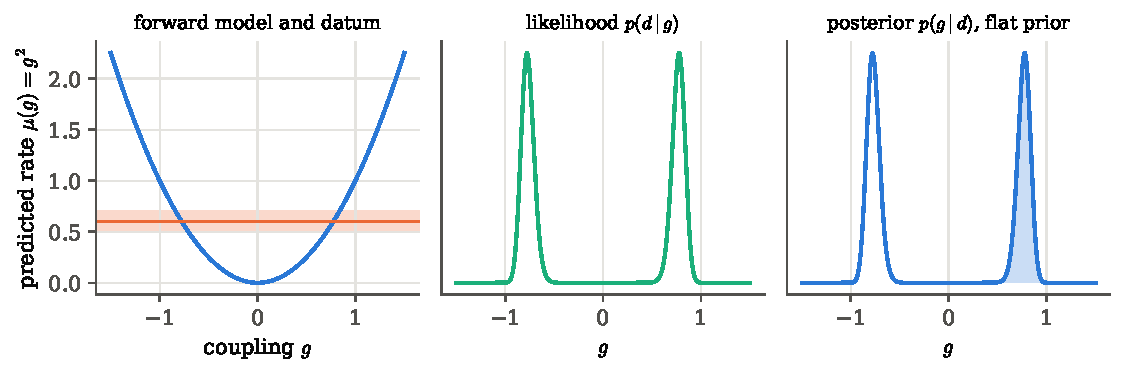
\includegraphics[width=\linewidth]{figures/ch05/grid_coupling.pdf}
\caption{Inferring a coupling from a rate proportional to its square. Left: the
forward model $g^2$ and the measured rate with its noise band. Two ranges of $g$, one
on each side of zero, predict rates inside the band. Middle: the likelihood as a
function of $g$ has a peak at each of them. Right: with a flat prior the posterior has
the same two peaks, and the shaded half, $g>0$, holds exactly half the probability.}
\label{5b:fig:coupling}
\end{figure}

\subsection{Many data points}

A real experiment gives many readings. Let the model predict a whole data vector
$\bm m(\lambda)=(m_1(\lambda),\dots,m_N(\lambda))$ and let the measured values be
$\data=(d_1,\dots,d_N)$ with independent Gaussian noise of sizes $\sigma_i$.
Independence means the joint density of all readings
is the product of the single-reading densities \mainref{p.~177}, so
\begin{align}
  \ln\Like(\lambda)
  &\eqby{1}\ln\prod_{i=1}^N\frac{1}{\sqrt{2\pi\sigma_i^2}}
     \exp\!\left[-\frac{(d_i-m_i(\lambda))^2}{2\sigma_i^2}\right]
   \nonumber\\
  &\eqby{2}-\frac12\sum_{i=1}^N\frac{(d_i-m_i(\lambda))^2}{\sigma_i^2}
     -\frac12\sum_{i=1}^N\ln(2\pi\sigma_i^2)
   \;=\;-\frac12\chi^2(\lambda)+\text{const}.
  \label{5b:eq:chi2}
\end{align}
\begin{explain}
  \item The likelihood of independent readings is the product of
        \eqref{5b:eq:gauss-like} over $i$.
  \item The log of a product is the sum of the logs, and $\ln e^{x}=x$.
\end{explain}
Here $\chi^2(\lambda)=\sum_i(d_i-m_i(\lambda))^2/\sigma_i^2$ is the sum of squared
residuals, each measured in units of its error bar, and the constant does not depend on
$\lambda$. With correlated noise of covariance matrix
$\Cmat$ the product is replaced by one multivariate Gaussian and
$\chi^2=(\data-\bm m)\T\Cmat^{-1}(\data-\bm m)$ (\cref{ch:03}). Either way the posterior
is
\begin{equation}
  p(\lambda\given\data)\propto e^{-\chi^2(\lambda)/2}\,p(\lambda),
  \label{5b:eq:post-chi2}
\end{equation}
and nothing in the logic has changed. The observed event is now the whole vector
$\data$. Each hypothesis $\lambda$ is judged by how plausible the whole vector of
fluctuations $\data-\bm m(\lambda)$ that it requires would be. Only the model for the
probability of the data changes from problem to problem. With a flat prior, $p(\lambda)$
is a constant, so the peak of the posterior is where $\chi^2$ is smallest: the
least-squares estimate. Least squares is therefore the special case ``flat prior,
Gaussian noise'' of Bayesian estimation \srcref{Sivia}{\S3.5}.

The same reasoning works at the scale of a whole survey; only the space of hypotheses
grows. In cosmology $\data$ may be thousands of band powers of the CMB and $\lambda$ the
handful of parameters of the standard cosmological model (see the cosmology notes). What we observed is the whole data
vector $\data$, every band power at once. The candidate explanations are the
possible values of $\lambda$, each one a different cosmological model. For each
of them the likelihood asks: had nature picked this model, how plausible would
it have been for exactly the data we hold to come out? Bayes' theorem combines
these likelihoods with the prior distribution and returns a posterior
distribution over the models.

\subsection{The posterior on a grid}

For one or two parameters the safest way to compute a posterior is to evaluate it on a
grid of values and look \srcref{Sivia}{\S3.4, ``brute force and ignorance''}. The grid
works whether the posterior is skewed, has several peaks, or has a sharp edge where the
prior stops. Its one trap is numerical: a product of many likelihoods is too large or
too small for a computer to store.

\paragraph{Example: a lifetime from 2000 readings.}
A source decays with lifetime $\tau$. We record the signal at $N=\FiveBTauN$ times,
$d_i=e^{-t_i/\tau}+\epsilon_i$ with $\sigma=\FiveBTauSigd$, and put a flat prior on
$\tau$. The obvious code multiplies the $N$ Gaussian densities for each grid value of
$\tau$. Each density near the curve is about $1/(\sqrt{2\pi}\,\sigma)\approx8$, and
$8^{2000}$ is far beyond the largest floating-point number, so the product comes out
as $\FiveBTauRawMax$. Now quote the same data in per cent. Every density is a hundred
times smaller, about $0.08$, and the product underflows to $\FiveBTauRawMaxPct$. The
posterior cannot depend on the units the data are quoted in, so neither answer means
anything. The cure is to work with logarithms \srcref{Sivia}{p.~34}:
\begin{enumerate}
  \item compute $L_j=\ln\Like(\tau_j)+\ln p(\tau_j)$ on the grid, as a \emph{sum} of
        logs;
  \item subtract the largest value, $L_j\to L_j-L_{\max}$, so that the largest is $0$;
  \item exponentiate, $w_j=e^{L_j-L_{\max}}$, which lies between $0$ and $1$;
  \item normalise, $p(\tau_j\given\data)=w_j/\sum_kw_k\Delta\tau$.
\end{enumerate}
Step 2 is legitimate because it multiplies every $w_j$ by the same constant
$e^{-L_{\max}}$, and a common constant cancels in the normalisation of step 4. For our
data $L_{\max}=\FiveBTauLogLmax$: the likelihood at the peak is $e^{\FiveBTauLogLmax}$,
a number no computer stores, but the \emph{ratios} of likelihoods between grid points
are perfectly ordinary numbers.

\pyfile[firstline=58,lastline=74,firstnumber=58]{code/ch05/08_grid_posterior.py}{The
lifetime posterior on a grid: the raw product fails, the log-sum with the maximum
subtracted works}

Line~63 builds the model prediction for every grid value of $\tau$ at every time at
once, as an $801\times2000$ array, and line~64 the Gaussian density of every reading.
Lines~65--68 form the raw products and show them overflow and, in per cent, underflow.
Line~69 is the log-likelihood as a sum, line~71 subtracts the maximum and
exponentiates, line~72 normalises, and lines~73--74 compute the posterior mean and
standard deviation by summing over the grid. The result is
$\tau=\FiveBTauMean\pm\FiveBTauSd$ (\cref{5b:fig:lifetime}), consistent with the true
value $2$ used in the simulation.

\begin{figure}[htbp]
\centering
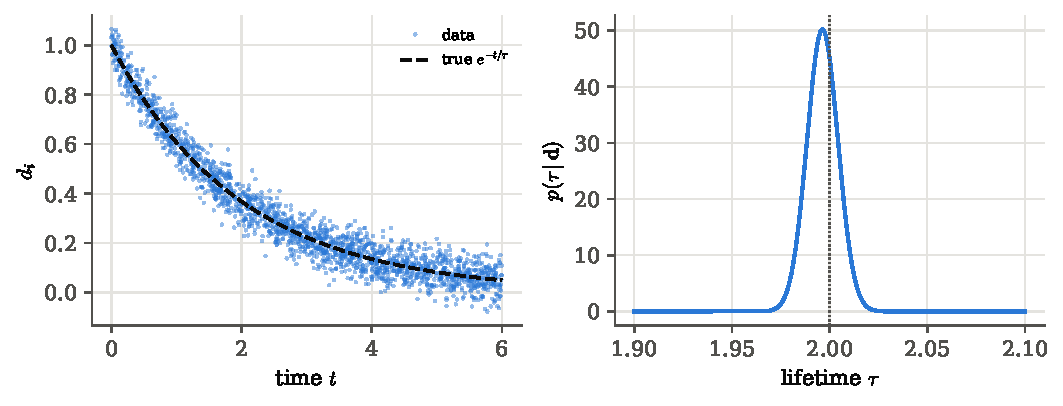
\includegraphics[width=0.9\linewidth]{figures/ch05/grid_lifetime.pdf}
\caption{A lifetime from 2000 noisy readings. Left: the readings (dots) and the true
decay curve (dashed). Right: the posterior for the lifetime computed on a grid of 801
values by summing log-likelihoods and subtracting their maximum. The dotted line marks
the value used to simulate the data.}
\label{5b:fig:lifetime}
\end{figure}

\begin{pitfall}[Never multiply raw likelihoods]
The product of many densities overflows or underflows depending only on the units the
data are quoted in. Always sum log-likelihoods and subtract the maximum before
exponentiating. The same rule applies to every sampler of \cref{ch:09}: they compare
$\ln p$ values, never $p$ values.
\end{pitfall}

A grid fails in many dimensions, because its cost grows as a power of the number of
parameters. With $n$ points per axis, a posterior in $D$ parameters needs $n^D$
evaluations: 100 points per axis is $10^4$
evaluations in two dimensions and $10^{12}$ in six, the size of a minimal cosmological
model. That cost, and the evidence integral it makes impossible, are what drive us to
sampling methods (\cref{ch:06,ch:09}).
\section{Conjugate priors: posteriors on the back of an envelope}
\label{5b:sec:conjugate}

For the likelihoods physicists meet most often, the product ``likelihood times prior''
can be worked out on paper. These are counts of successes, counts of events and
Gaussian readings. A grid (\cref{5b:sec:continuous}) also gives the posterior, but only
as a table of numbers. On paper the posterior comes out in the same family of curves as
the prior, with a few constants shifted by the data. We can then see at a glance how
much of the answer comes from the data and how much from the prior. Updating becomes
bookkeeping: add the number of heads here, the number of counts there.

The question is: for which pairs of likelihood and prior does the product have the same
functional form as the prior, and what are the update rules?

\begin{workdef}[conjugate prior]
A family of prior densities is \newterm{conjugate} to a likelihood if, for every data
set, prior from the family $\times$ likelihood is again a member of the family
\unpack{same functional form in the parameter, different values of its constants}
\mainref{p.~179}. Conjugacy is a property of the \emph{pair}: a prior is conjugate only
with respect to a particular likelihood \srcref{Kruschke}{\S6.2}. \emph{Operationally:}
write the likelihood as a function of the parameter, drop every factor that does not
contain it, and look for a density with the same $\theta$-dependence.
\end{workdef}

\subsection{Coins: the Beta--Binomial pair}

A coin, or any process with two outcomes, has unknown probability $\theta$ of
``success''. One toss $y\in\{0,1\}$ has the Bernoulli probability
$\theta^y(1-\theta)^{1-y}$, and $N$ independent tosses with $z$ successes have
\srcref{Kruschke}{(6.2)}
\begin{align*}
  p(\{y_i\}\given\theta)
  \eqby{1}\prod_{i=1}^N\theta^{y_i}(1-\theta)^{1-y_i}
  \eqby{2}\theta^{\sum_iy_i}(1-\theta)^{\sum_i(1-y_i)}
  =\theta^{z}(1-\theta)^{N-z}.
\end{align*}
\begin{explain}
  \item Independent tosses: the joint probability is the product.
  \item Powers of the same base multiply by adding exponents.
\end{explain}
As a function of $\theta$ this is a power of $\theta$ times a power of $1-\theta$. A
prior of the same shape is the \newterm{Beta distribution} (\cref{ch:02}),
\begin{equation}
  p(\theta)=\mathrm{Beta}(\theta\given a,b)=\frac{\theta^{a-1}(1-\theta)^{b-1}}{B(a,b)},
  \qquad
  B(a,b)=\int_0^1\theta^{a-1}(1-\theta)^{b-1}\dd\theta=\frac{\Gamma(a)\Gamma(b)}{\Gamma(a+b)},
  \label{5b:eq:beta}
\end{equation}
with $a,b>0$ \srcref{Kruschke}{(6.3)--(6.4)}. The Beta function $B(a,b)$ is only a
normalising number. Recall $\Gamma(n)=(n-1)!$ for integers and $\Gamma(x+1)=x\Gamma(x)$
in general. The flat prior is $\mathrm{Beta}(1,1)$. Multiply prior and likelihood:
\begin{align}
  p(\theta\given z,N)
  &\eqby{1}\frac{\theta^{z}(1-\theta)^{N-z}\;\theta^{a-1}(1-\theta)^{b-1}/B(a,b)}{p(z,N)}
   \eqby{2}\frac{\theta^{(z+a)-1}(1-\theta)^{(N-z+b)-1}}{B(a,b)\,p(z,N)}
   \nonumber\\
  &\eqby{3}\frac{\theta^{(z+a)-1}(1-\theta)^{(N-z+b)-1}}{B(z+a,\,N-z+b)}
   =\mathrm{Beta}(\theta\given z+a,\;N-z+b).
  \label{5b:eq:beta-post}
\end{align}
\begin{explain}
  \item Bayes' theorem with the Bernoulli likelihood and the Beta prior.
  \item Collect the powers of $\theta$ and of $1-\theta$.
  \item The numerator is the $\theta$-dependence of a Beta density with parameters
        $z+a$ and $N-z+b$. A density must integrate to one, and there is only one
        constant that makes this one do so, $B(z+a,N-z+b)$. So the denominator must be
        that constant, and no integral was needed \srcref{Kruschke}{\S6.3}.
\end{explain}
The update rule is: \emph{add the successes to $a$ and the failures to $b$}. Adding is
done in any order, so the result is the same whether the tosses arrive one at a time
or all at once, as sequential updating requires (\cref{5a:sec:sequential}). The rule
also tells us how to read a prior. $\mathrm{Beta}(a,b)$ behaves like the posterior we
would hold after seeing about $a$ successes and $b$ failures. So $\kappa=a+b$ counts how
many tosses' worth of information the prior carries \srcref{Kruschke}{\S6.2.1}.

\paragraph{The posterior mean is a compromise.}
The mean of a Beta density is
\begin{align*}
  \E[\theta]
  \eqby{1}\frac{1}{B(a,b)}\int_0^1\theta^{a}(1-\theta)^{b-1}\dd\theta
  \eqby{2}\frac{B(a+1,b)}{B(a,b)}
  \eqby{3}\frac{\Gamma(a+1)\,\Gamma(a+b)}{\Gamma(a)\,\Gamma(a+b+1)}
  \eqby{4}\frac{a}{a+b}.
\end{align*}
\begin{explain}
  \item Definition of the mean, $\int\theta\,p(\theta)\dd\theta$, with one extra power
        of $\theta$.
  \item The integral is the Beta function with $a\to a+1$.
  \item Write both Beta functions with Gammas. $\Gamma(b)$ cancels.
  \item $\Gamma(a+1)=a\Gamma(a)$ and $\Gamma(a+b+1)=(a+b)\Gamma(a+b)$.
\end{explain}
For the posterior \eqref{5b:eq:beta-post} this gives \srcref{Kruschke}{(6.9)},
\mainref{p.~179}
\begin{align}
  \frac{z+a}{N+a+b}
  \eqby{1}\frac{z}{N}\cdot\frac{N}{N+a+b}+\frac{a}{a+b}\cdot\frac{a+b}{N+a+b} .
  \label{5b:eq:beta-mean}
\end{align}
\begin{explain}
  \item Multiply out the right side: the $N$ and the $a+b$ cancel, leaving
        $(z+a)/(N+a+b)$.
\end{explain}
The posterior mean is a weighted average of two numbers: the observed fraction $z/N$
(the maximum likelihood estimate) and the prior mean $a/(a+b)$. Their weights are
proportional to the number of tosses $N$ and to the prior's worth in tosses,
$\kappa=a+b$. So the data win once $N\gg\kappa$. For a flat prior, $a=b=1$, it is
$(z+1)/(N+2)$, Laplace's rule of succession \mainref{p.~178, (11.5)--(11.6)}. For
example, Kruschke's prior $\mathrm{Beta}(5,5)$ with $z=1$ success in $N=10$ gives
posterior mean $(1+5)/(10+10)=0.3$, exactly halfway between the prior mean $0.5$ and the
data fraction $0.1$, because $N=\kappa$ \srcref{Kruschke}{Fig.~6.3}.

\paragraph{Example: the same data, three priors.}
\emph{The event.} A two-outcome process is tried 20 times and gives 17 successes, 85\%.
\emph{The question.} What should we now believe about its success probability $\theta$?
The answer depends on what we knew before, that is, on what the process is
\srcref{Kruschke}{\S6.4.1}.
\emph{Three cases in turn.} If it is a freshly minted government coin, we are confident
it is fair: prior $\mathrm{Beta}(100,100)$, worth 200 tosses of evidence for $0.5$. If a
success is a professional basketball player making a free throw, we know such players
make about 75\% of them: prior $\mathrm{Beta}(18.25,6.75)$, mode $0.75$ and $\kappa=25$.
If it is the colour of samples of a substance on a distant planet, we know only that
both outcomes are possible: $\mathrm{Beta}(1,1)$.
\emph{Only then the numbers.} Adding 17 to $a$ and 3 to $b$, the three posteriors are $\mathrm{Beta}(117,103)$,
$\mathrm{Beta}(35.25,9.75)$ and $\mathrm{Beta}(18,4)$, with modes
$\FiveBBetaModeS$, $\FiveBBetaModeL$ and $\FiveBBetaModeF$ (\cref{5b:fig:three-priors}).
The 17 successes barely move the government coin, pull the basketball player just above his
league's typical rate, and fully determine the planetary substance. None of the three
analysts is wrong. They started from different knowledge, and twenty tosses are not
enough to overwhelm a prior worth two hundred.

\begin{figure}[htbp]
\centering
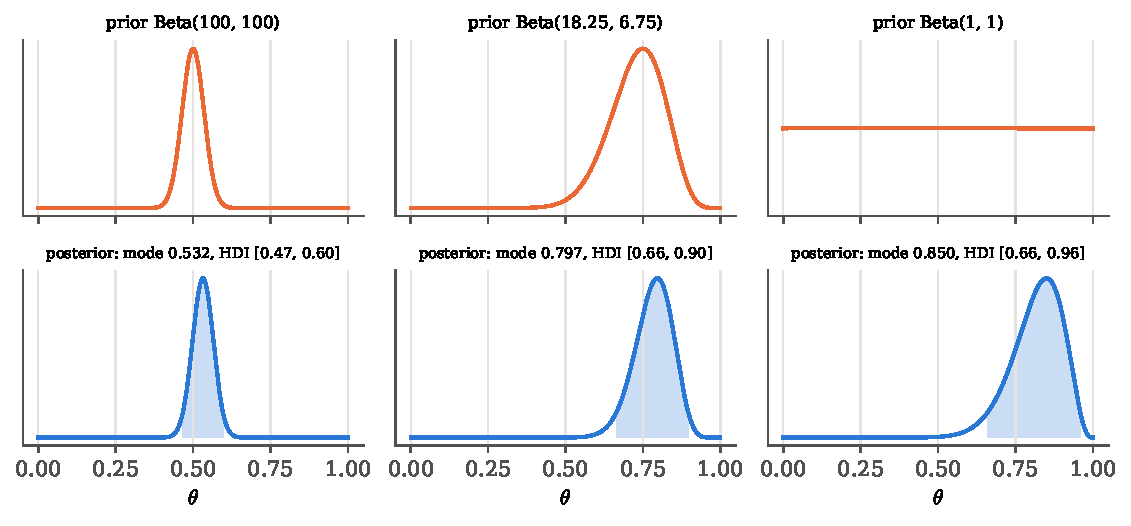
\includegraphics[width=\linewidth]{figures/ch05/conjugate_three_priors.pdf}
\caption{Seventeen heads in twenty tosses, analysed with three priors. Top row: a
confident fair-coin prior, a basketball league's free-throw rate, and a flat prior.
Bottom row: the three posteriors, each a Beta density, with the shaded 95\% highest
density interval (\cref{5b:sec:summaries}). The same data move the three beliefs by
very different amounts.}
\label{5b:fig:three-priors}
\end{figure}

\paragraph{Example: predicting the next two tosses.}
Conjugacy also gives predictions in closed form. A coin gave 10 heads in 14 tosses. What
is the probability that the next two tosses are both heads \srcref{Padilla}{\S2.3,
\S3.1}? With a flat prior, $\mathrm{Beta}(1,1)$, the posterior is $\mathrm{Beta}(1+10,
1+4)=\mathrm{Beta}(11,5)$. If we knew $\theta$, two heads would have probability
$\theta^2$. We do not know $\theta$, so we average $\theta^2$ over the posterior, that
is, we marginalise $\theta$:
\begin{align*}
  \Prob(\text{HH}\given\data)
  \eqby{1}\int_0^1\theta^2\,\frac{\theta^{10}(1-\theta)^{4}}{B(11,5)}\,\dd\theta
  \eqby{2}\frac{B(13,5)}{B(11,5)}
  \eqby{3}\frac{12\cdot11}{17\cdot16}
  =\FiveBPred .
\end{align*}
\begin{explain}
  \item Sum over the paths ``$\theta$, then two heads'': the probability of HH given
        $\theta$ times the posterior density of $\theta$.
  \item The integral is a Beta function with the first argument raised by two.
  \item $B(13,5)/B(11,5)=\Gamma(13)\Gamma(16)/[\Gamma(11)\Gamma(18)]$, and
        $\Gamma(13)/\Gamma(11)=12\cdot11$, $\Gamma(18)/\Gamma(16)=17\cdot16$.
\end{explain}
Plugging in the single best value $\hat\theta=10/14$ instead gives
$(10/14)^2=\FiveBPlugin$. The posterior predictive is smaller, and it is the honest
answer. It remembers that $\theta$ might be lower than $10/14$; the plug-in pretends that
14 tosses fixed $\theta$ exactly.

\subsection{Counts: the Gamma--Poisson pair}

A detector counts cosmic-ray muons in one-minute windows. The counts $n_1,\dots,n_M$ are
Poisson with unknown rate $\lambda$ per minute, so the likelihood is
\srcref{Lambert}{(9.8)}
\begin{align*}
  p(\{n_i\}\given\lambda)
  \eqby{1}\prod_{i=1}^M\frac{\lambda^{n_i}e^{-\lambda}}{n_i!}
  \eqby{2}\frac{\lambda^{\sum_in_i}\,e^{-M\lambda}}{\prod_in_i!}
  \;\propto\;\lambda^{S}e^{-M\lambda},\qquad S=\sum_in_i .
\end{align*}
\begin{explain}
  \item Independent windows: the product of Poisson probabilities.
  \item Add the exponents of $\lambda$, and $M$ copies of $e^{-\lambda}$ make
        $e^{-M\lambda}$. The factorials do not contain $\lambda$.
\end{explain}
A power of $\lambda$ times a decaying exponential in $\lambda$ is the shape of the
\newterm{Gamma distribution}, $\mathrm{Gamma}(\lambda\given\alpha,\beta)=\beta^\alpha
\lambda^{\alpha-1}e^{-\beta\lambda}/\Gamma(\alpha)$ for $\lambda>0$, with mean
$\alpha/\beta$ and variance $\alpha/\beta^2$ (\cref{ch:02}). Multiplying,
\begin{align}
  p(\lambda\given\{n_i\})
  \eqby{1}\lambda^{S}e^{-M\lambda}\cdot\lambda^{\alpha-1}e^{-\beta\lambda}
  \eqby{2}\lambda^{(\alpha+S)-1}e^{-(\beta+M)\lambda}
  \;\Rightarrow\;
  \lambda\given\{n_i\}\sim\mathrm{Gamma}(\alpha+S,\;\beta+M).
  \label{5b:eq:gamma-post}
\end{align}
\begin{explain}
  \item Posterior $\propto$ likelihood $\times$ prior, dropping constants.
  \item Collect powers and exponents. The normalisation follows as in the Beta case.
\end{explain}
The rule is: \emph{add the total count to $\alpha$ and the number of windows to $\beta$}
\srcref{Lambert}{(9.11)}. So $\mathrm{Gamma}(\alpha,\beta)$ is like having already seen
about $\alpha$ counts in $\beta$ windows, and the posterior mean $(\alpha+S)/(\beta+M)$ is
again a weighted average, of the prior mean $\alpha/\beta$ and the observed mean $S/M$.

\paragraph{Example: the muon rate.}
A previous run suggested ``about 3 per minute, not very sure'': prior
$\mathrm{Gamma}(3,1)$, mean 3, standard deviation $\sqrt3\approx1.7$. Five windows gave
$\FiveBCountsList$ counts, total $S=\FiveBCountsSum$, observed mean $\FiveBGamMLE$. The
posterior is $\mathrm{Gamma}(\FiveBGamA,\FiveBGamB)$ with mean $\FiveBGamMean$ and
standard deviation $\FiveBGamSd$: pulled a little from the data's $\FiveBGamMLE$ towards
the prior's 3, since the prior is worth one window against the data's five
(\cref{5b:fig:conjugate}, middle).

\subsection{Gaussian readings: inverse-variance weighting emerges}

Several laboratories measure the same quantity $\mu$ with different instruments. Reading
$x_k$ has Gaussian error $\sigma_k$, and we have a Gaussian prior $\Normal(a,b^2)$ of
mean $a$ and width $b$. We work with the logarithm, because the log of a product of
Gaussians is a sum of squares, which is easy to collect. Up to constants that do not
contain $\mu$,
\begin{align}
  -2\ln p(\mu\given\{x_k\})
  &\eqby{1}\sum_k\frac{(x_k-\mu)^2}{\sigma_k^2}+\frac{(\mu-a)^2}{b^2}
   \nonumber\\
  &\eqby{2}\mu^2\Bigl(\sum_kw_k+\frac1{b^2}\Bigr)
     -2\mu\Bigl(\sum_kw_kx_k+\frac{a}{b^2}\Bigr)+\text{const}
   \nonumber\\
  &\eqby{3}P\,(\mu-m)^2+\text{const},\qquad
   P=\sum_kw_k+\frac1{b^2},\quad m=\frac{\sum_kw_kx_k+a/b^2}{P}.
  \label{5b:eq:normal-post}
\end{align}
\begin{explain}
  \item Log of Gaussian likelihoods times a Gaussian prior, multiplied by $-2$.
  \item Expand the squares and write $w_k=1/\sigma_k^2$. Terms without $\mu$ go into
        the constant.
  \item Complete the square: $P\mu^2-2\mu Pm=P(\mu-m)^2-Pm^2$, and $Pm^2$ is a constant.
\end{explain}
The posterior is therefore Gaussian, $\mu\given\{x_k\}\sim\Normal(m,1/P)$
\mainref{p.~179, (11.7)}. Two rules have appeared by themselves.
\begin{itemize}
  \item \emph{Precisions add.} The precision (inverse variance) of the posterior is
        the sum of the precisions of the measurements and of the prior.
  \item \emph{Means are precision-weighted.} Each measurement counts in proportion to
        $1/\sigma_k^2$, and the prior counts as one more measurement, of value $a$ and
        error $b$.
\end{itemize}
With a very broad prior, $b\to\infty$, we get the familiar inverse-variance weighted
mean $\bar\mu=\sum_kw_kx_k/\sum_kw_k$ with error $(\sum_kw_k)^{-1/2}$
\srcref{Sivia}{(2.30)--(2.31)}. For $N$ equal errors this is the sample mean with error
$\sigma/\sqrt N$. Wasserman writes the same result as $m=w\bar X+(1-w)a$ with
$w=(1/\mathrm{se}^2)/(1/\mathrm{se}^2+1/b^2)$ and $\mathrm{se}=\sigma/\sqrt n$
\mainref{p.~179}.

\paragraph{Example: three laboratories.}
Three simulated measurements are $\FiveBNxa\pm0.5$, $\FiveBNxb\pm1.0$ and
$\FiveBNxc\pm2.0$, and a vague earlier estimate gives the prior $\Normal(8,3^2)$. The
posterior is $\mu=\FiveBNmPost\pm\FiveBNsPost$. Without the prior, the inverse-variance
weighted mean is $\FiveBNmIvw\pm\FiveBNsIvw$. The prior counts as one more measurement,
of error 3. It shifts the answer by a tenth of its error bar and shrinks the error bar
slightly (\cref{5b:fig:conjugate}, right).

\begin{figure}[htbp]
\centering
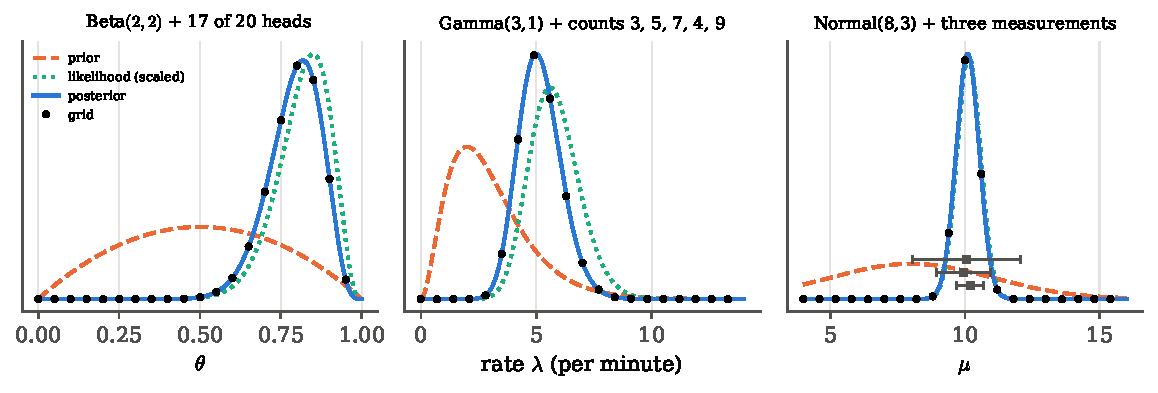
\includegraphics[width=\linewidth]{figures/ch05/conjugate_pairs.pdf}
\caption{The three conjugate pairs. In each panel the dashed curve is the prior, the
dotted curve the likelihood (scaled to unit area), the solid curve the closed-form
posterior and the dots the posterior computed by brute force on a grid. Left: a Beta
prior and 17 heads in 20. Middle: a Gamma prior and five minutes of muon counts.
Right: a Gaussian prior and three measurements with different error bars (squares with
bars). The dots lie on the curves, to a relative accuracy of $10^{-11}$.}
\label{5b:fig:conjugate}
\end{figure}

The update rules are exact, and the grid check in \cref{5b:fig:conjugate} confirms it.
The largest relative difference between the brute-force and closed-form posteriors is
$\FiveBBetaErr$ for the Beta case, $\FiveBGamErr$ for the Gamma case and $\FiveBNErr$ for
the Gaussian case: pure round-off.

\begin{taxonomy}[common conjugate pairs]
\centering\small
\begin{tabular}{@{}lll@{}}
\toprule
likelihood (data) & conjugate prior & posterior \\
\midrule
Bernoulli/binomial ($z$ of $N$) & $\mathrm{Beta}(a,b)$ & $\mathrm{Beta}(a+z,\,b+N-z)$\\
Poisson (total $S$ in $M$ windows) & $\mathrm{Gamma}(\alpha,\beta)$ & $\mathrm{Gamma}(\alpha+S,\,\beta+M)$\\
multinomial (counts $\bm n$) & $\mathrm{Dirichlet}(\bm\alpha)$ & $\mathrm{Dirichlet}(\bm\alpha+\bm n)$\\
Gaussian, known $\sigma_k$ & $\Normal(a,b^2)$ & $\Normal(m,1/P)$, \eqref{5b:eq:normal-post}\\
Gaussian, known mean, variance $v$ & $\text{Inv-Gamma}(\alpha,\beta)$ &
  $\text{Inv-Gamma}\bigl(\alpha+\frac N2,\,\beta+\frac12\sum(x_i-\mu)^2\bigr)$\\
\bottomrule
\end{tabular}
\par\smallskip\raggedright
Sources: \srcref{Lambert}{Table~9.1}, \mainref{pp.~178--179}. The last row is the one
used for a power-spectrum amplitude below.
\end{taxonomy}

\paragraph{The limits of conjugacy.}
Conjugate pairs exist only for a handful of simple likelihoods, and even then only
priors of one particular shape are allowed. A coin factory that makes coins biased
either near $0.25$ or near $0.75$ has a two-humped prior that no Beta density can
represent. Its posterior after 14 heads in 27 has three bumps, a compromise between the
two humps of the prior and the single peak of the likelihood, and must be computed on a
grid \srcref{Kruschke}{\S6.4.2}. Likewise, replacing a Gaussian likelihood by a more
robust Student-$t$ destroys conjugacy altogether \srcref{Lambert}{\S9.7}. The lesson is
not to bend the model to fit a conjugate prior. Conjugacy is a source of exact test
cases and of intuition. Realistic models are handled by grids in low dimension and by
sampling (\cref{ch:09}) in high dimension.

\subsection{One calculation, three instruments}

The same few lines of algebra appear in three very different corners of physics. Only
the likelihood changes: counts at a collider are Poisson, a CMB map is a Gaussian random
field, and a gravitational-wave strain is a known waveform in Gaussian noise described
by a power spectral density (\cref{5b:fig:instruments}).

\paragraph{A collider search with no background.}
A search for a rare process expects $s$ signal events and, after cuts, essentially no
background. The number observed is Poisson with mean $s$. Suppose nothing is seen. How
large could $s$ be? The flat prior on $s\ge0$ is the $\mathrm{Gamma}(1,0)$ limit, and
the search is a single window, so the Gamma update \eqref{5b:eq:gamma-post} with $n$
events gives $s\given n\sim\mathrm{Gamma}(n+1,1)$. For $n=0$ the posterior is $e^{-s}$.
The 95\% credible upper limit $s_{95}$ is the value below which $s$ lies with
probability 95\%, so it solves
\begin{align*}
  0.95\eqby{1}\int_0^{s_{95}}e^{-s}\,\dd s\eqby{2}1-e^{-s_{95}}
  \quad\Rightarrow\quad s_{95}=\ln 20=\FiveBULzero .
\end{align*}
\begin{explain}
  \item The posterior probability that $s$ is below the limit is 95\%.
  \item Elementary integral.
\end{explain}
This is the famous ``three events'' upper limit for an empty search. With one or three
events observed the limits are $\FiveBULone$ and $\FiveBULthree$.

\paragraph{The CMB: a power-spectrum amplitude from $2\ell+1$ numbers.}
The temperature map is expanded in spherical harmonics, and at multipole $\ell$ the
coefficients $\alm$ amount to $2\ell+1$ independent real Gaussian numbers of zero mean
and variance $\Cell$ (see the cosmology notes, and \cref{ch:07}). Their likelihood is
\begin{align*}
  p(\{\alm\}\given\Cell)
  \eqby{1}\prod_{m=-\ell}^{\ell}\frac{e^{-|\alm|^2/2\Cell}}{\sqrt{2\pi\Cell}}
  \;\propto\;\Cell^{-(2\ell+1)/2}\exp\!\left[-\frac{(2\ell+1)\Chat}{2\Cell}\right],
  \qquad \Chat=\frac{1}{2\ell+1}\sum_m|\alm|^2 .
\end{align*}
\begin{explain}
  \item $2\ell+1$ independent Gaussians of variance $\Cell$, and the sum of their squares
        written through the estimator $\Chat$.
\end{explain}
As a function of $\Cell$ this is an inverse power times $e^{-\text{const}/\Cell}$. That
is the shape of an inverse-Gamma density, the last row of the table. With the scale-invariant prior
$p(\Cell)\propto1/\Cell$ (\cref{5b:sec:priors}) the posterior is
$\text{Inv-Gamma}\bigl(\tfrac{2\ell+1}2,\tfrac{(2\ell+1)\Chat}2\bigr)$. For the
quadrupole, $\ell=2$, only five numbers exist in the whole sky. The posterior of
$\Cell/\Chat$ has its mode at $\FiveBCmbModeTwo$, its mean at $\FiveBCmbMeanTwo$, and its
central 68\% interval from $\FiveBCmbLoTwo$ to $\FiveBCmbHiTwo$. So five numbers cannot
pin the quadrupole power to better than a factor of about two, however good the
telescope. This is cosmic variance seen as a posterior. At $\ell=50$ the interval has shrunk to
$[\FiveBCmbLoFifty,\FiveBCmbHiFifty]$ and the posterior is nearly Gaussian.

\paragraph{A gravitational-wave amplitude.}
A detector records $d=A\,h_0+n$, where $h_0$ is a known waveform, $A$ an unknown
amplitude and $n$ stationary Gaussian noise with power spectral density $S_n(f)$. The
likelihood is $\Like\propto\exp[-\frac12(d-Ah_0\,|\,d-Ah_0)]$ with the noise-weighted
inner product $(a|b)=4\,\mathrm{Re}\int_0^\infty\tilde a\tilde b^*/S_n\,\dd f$
(\cref{ch:03}). The inner product is linear in each slot, so
\begin{align*}
  (d-Ah_0\,|\,d-Ah_0)
  \eqby{1}(d|d)-2A\,(d|h_0)+A^2\,(h_0|h_0)
  \eqby{2}(h_0|h_0)\,\bigl(A-\hat A\bigr)^2+\text{const},
  \\ \hat A=\frac{(d|h_0)}{(h_0|h_0)} .
\end{align*}
\begin{explain}
  \item Expand, using $(h_0|d)=(d|h_0)$ for the real inner product.
  \item Complete the square in $A$.
\end{explain}
The posterior for $A$ with a flat or Gaussian prior is Gaussian, centred on the
matched-filter estimate $\hat A$, with standard deviation $1/\sqrt{(h_0|h_0)}$. For our
toy chirp in coloured noise, normalised to $(h_0|h_0)=\FiveBGwHH$, the posterior is
$A=\FiveBGwAhat\pm\FiveBGwAsd$ for true $A=1$, and over 4000 independent noise
realisations the estimate $\hat A$ scatters by $\FiveBGwSpread$, the posterior width, as
it should.

\begin{figure}[htbp]
\centering
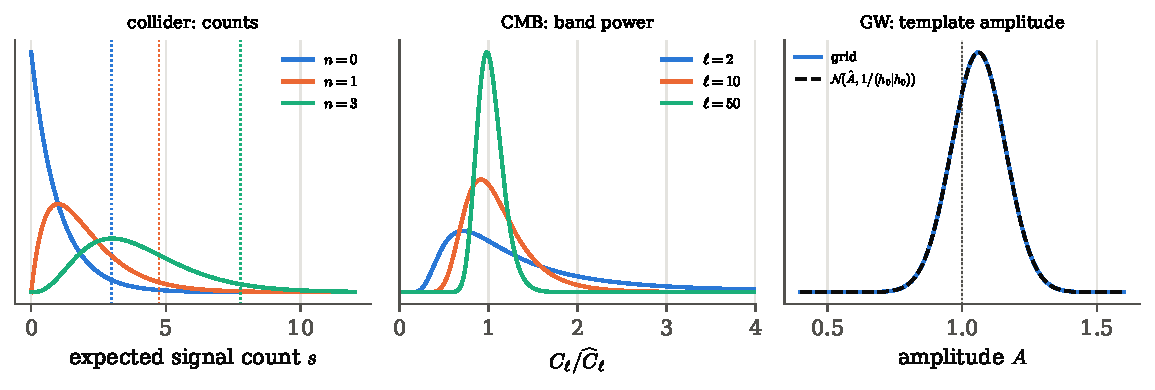
\includegraphics[width=\linewidth]{figures/ch05/three_instruments.pdf}
\caption{One posterior calculation in three instruments. Left: a background-free
collider search, posterior for the expected signal after 0, 1 and 3 observed events,
with the 95\% upper limits dotted. Middle: the posterior of a CMB band power relative to
its estimate, for $\ell=2$, 10 and 50. The quadrupole's posterior is broad and skewed.
Right: the amplitude of a known gravitational-wave template in coloured noise, computed
on a grid (solid) and from the closed form (dashed).}
\label{5b:fig:instruments}
\end{figure}

\begin{inpractice}[closed forms inside large analyses]
Conjugate results survive as building blocks inside big pipelines. Collider limits for
counting experiments are routinely quoted as Bayesian upper limits with a flat prior on
the signal rate, exactly the Gamma calculation above, and physicists check them against
frequentist constructions (\cref{ch:04}). CMB likelihoods at low $\ell$ use the exact
inverse-Gamma shape rather than a Gaussian, because the quadrupole's posterior is far
from Gaussian (\cref{ch:07}). Gravitational-wave pipelines marginalise analytically over
parameters that enter linearly, such as an amplitude or a phase, before sampling the
rest (\cref{ch:09}). Everywhere, the closed forms are also the test cases that a new
sampler must reproduce.
\end{inpractice}
\section{Summarising a posterior: best values and credible intervals}
\label{5b:sec:summaries}

The posterior is the complete answer: every statement we can make about the parameter
is an integral of it. But papers quote only a handful of numbers, such as
``$\theta=0.28\pm0.08$'' or ``$s<3$ events at 95\%''. A decision, such as building the
next detector or claiming a discovery, also needs one number or one interval. So which
numbers should we quote, and what exactly does each one mean?

Our running example is the posterior of the CMB quadrupole power $C_2$ from
\cref{5b:sec:conjugate}. There the five numbers $a_{2m}$ ($m=-2,\dots,2$) measured over
the whole sky gave an inverse-Gamma posterior. Write it in terms of the ratio
$x=C_2/\widehat C_2$ of the power to its estimate $\widehat C_2=\frac15\sum_m|a_{2m}|^2$.
Then its parameters are $\alpha=\beta=5/2$, and it is strongly skewed, with a long tail
to large $x$ (\cref{5b:fig:summaries}, left).

\subsection{Three best values, three losses}

There are three standard point summaries \srcref{Lambert}{\S7.6}: the
\newterm{posterior mean} $\E[\theta\given\data]=\int\theta\,p(\theta\given\data)
\dd\theta$ \mainref{p.~177, (11.4)}, the \newterm{posterior median} (half the
probability on each side), and the \newterm{posterior mode} or MAP, \emph{maximum a
posteriori}, the highest point of the density. For a symmetric single-peaked posterior
they coincide. For the quadrupole they are
\[
  \text{mode }\FiveBSumMode,\qquad\text{median }\FiveBSumMedian,\qquad
  \text{mean }\FiveBSumMean .
\]
Which one is ``right''? Each is the best answer to a different question: what does it
cost us to be wrong? Suppose we must announce one number $M$, and we pay a penalty
$\mathrm{loss}(\theta-M)$ if the truth turns out to be $\theta$. We do not know
$\theta$, so we average the penalty over the posterior. The expected penalty is
$R(M)=\int\mathrm{loss}(\theta-M)\,p(\theta\given\data)\,\dd\theta$, and the best $M$ is
the one that makes it smallest \srcref{Kruschke}{\S4.3.3}. We take three penalties in
turn.

\paragraph{Squared loss gives the mean.}
With $\mathrm{loss}=(\theta-M)^2$,
\begin{align*}
  \frac{\dd R}{\dd M}
  \eqby{1}\int\frac{\partial}{\partial M}(\theta-M)^2\,p(\theta\given\data)\,\dd\theta
  \eqby{2}-2\int(\theta-M)\,p(\theta\given\data)\,\dd\theta
  \eqby{3}-2\bigl(\E[\theta\given\data]-M\bigr),
\end{align*}
\begin{explain}
  \item Differentiate under the integral, since the limits do not depend on $M$.
  \item $\partial_M(\theta-M)^2=-2(\theta-M)$.
  \item Split the integral: $\int\theta p\,\dd\theta$ is the mean and $\int Mp\,\dd\theta
        =M$ because $p$ is normalised.
\end{explain}
which vanishes at $M=\E[\theta\given\data]$. A large miss costs the square of its size,
so the rare values far out in a long tail weigh heavily, and they drag the answer
towards that tail.

\paragraph{Absolute loss gives the median.}
With $\mathrm{loss}=|\theta-M|$,
\begin{align*}
  \frac{\dd R}{\dd M}
  \eqby{1}\int_{-\infty}^{M}p(\theta\given\data)\,\dd\theta
         -\int_{M}^{\infty}p(\theta\given\data)\,\dd\theta
  \eqby{2}\Prob(\theta<M\given\data)-\Prob(\theta>M\given\data),
\end{align*}
\begin{explain}
  \item $\partial_M|\theta-M|$ is $+1$ for $\theta<M$ and $-1$ for $\theta>M$.
  \item Each integral of the density over a half-line is a probability.
\end{explain}
which vanishes when half the probability lies on each side: the median.

\paragraph{``All or nothing'' gives the mode.}
If we win only when $M$ lands within a tiny window $\pm\delta$ of the truth, the
expected reward is $\int_{M-\delta}^{M+\delta}p\,\dd\theta\approx2\delta\,p(M\given
\data)$, largest where the density is highest: the MAP.

The mode is the easiest to compute. The evidence does not depend on $\theta$, so the
mode is simply the maximum of likelihood times prior, and no normalisation is needed.
With a flat prior it is the maximum-likelihood estimate. But it is the most fragile of
the three, for two reasons. First, it depends on the parametrisation: a density changes
shape when the axis is stretched (\cref{5b:sec:priors}). Second, for a skewed posterior
it can sit far from the bulk of the probability. For the quadrupole,
$\FiveBSumAboveMode$\% of the posterior probability lies \emph{above} the mode.

The median does not have the first weakness. If $y=g(\theta)$ is increasing, the median
of $y$ is $g$ of the median of $\theta$. The reason is that ``half the probability lies
below'' is a statement about the probabilities of corresponding intervals, and a change
of variable does not alter those. Lambert ranks the mean first, the median second and
the MAP last \srcref{Lambert}{\S7.6}. Whichever is quoted, say which one it is, and give
an interval with it.

\subsection{Credible intervals}

A \newterm{credible interval} of level $1-\alpha$ is any region holding posterior
probability $1-\alpha$. Many regions do so, and two conventions pick one of them.

The \newterm{equal-tailed interval} (ETI) puts probability $\alpha/2$ in each tail: find
$a,b$ with $\int_{-\infty}^ap\,\dd\theta=\int_b^\infty p\,\dd\theta=\alpha/2$
\mainref{p.~178}. It is the interval between two quantiles, easy to compute from a
cumulative distribution or from samples (\cref{5b:sec:sampling}), and, like the median,
it maps onto itself under any increasing change of variable.

The \newterm{highest density interval} (HDI) instead takes the most credible values
first \srcref{Kruschke}{\S4.3.4}. Picture the posterior curve as a landscape, with a
water level $W$ that is lowered from above. The HDI is the set of $\theta$ that stick out above the
water, $p(\theta\given\data)>W$, with $W$ lowered until that set holds probability
$1-\alpha$ (\cref{5b:fig:hdi-water}).

\begin{workdef}[highest density interval]
The $(1-\alpha)$ \newterm{HDI} is the set $\{\theta:\,p(\theta\given\data)>W\}$, where
the level $W$ is chosen so that $\int_{p>W}p(\theta\given\data)\,\dd\theta=1-\alpha$.
Every point inside has higher density than every point outside
\unpack{so it contains the most credible values}. For a single-peaked posterior it is
the \emph{shortest} interval with probability $1-\alpha$ \srcref{Sivia}{(2.21)}. For a
posterior with several peaks it can be several disjoint intervals.
\emph{Operationally:} on a grid, sort the grid values by density and accumulate them from
the top until the probability reaches $1-\alpha$. From samples, take the shortest
interval that contains a fraction $1-\alpha$ of the sorted samples.
\end{workdef}

\begin{figure}[htbp]
\centering
\begin{tikzpicture}[x=1.15cm,y=2.2cm]
  \def\dens(#1){0.55*exp(-(#1-1.6)^2/0.35)+0.38*exp(-(#1-4.6)^2/0.45)}
  \fill[formblue!18,domain=0.943:2.257,samples=60] (0.943,0) -- plot (\x,{\dens(\x)}) -- (2.257,0) -- cycle;
  \fill[formblue!18,domain=3.976:5.224,samples=60] (3.976,0) -- plot (\x,{\dens(\x)}) -- (5.224,0) -- cycle;
  \draw[form,domain=0:6.3,samples=160] plot (\x,{\dens(\x)});
  \draw[faint,->] (-0.1,0) -- (6.6,0) node[right,black,lbl] {$\theta$};
  \draw[bdryred,thick,dashed] (-0.1,0.16) -- (6.4,0.16);
  \node[lbl,bdryred,anchor=east] at (-0.15,0.16) {level $W$};
  \draw[very thick,formblue] (0.943,-0.08) -- (2.257,-0.08);
  \draw[very thick,formblue] (3.976,-0.08) -- (5.224,-0.08);
  \node[lbl,anchor=north] at (3.1,-0.14) {HDI $=$ two intervals, total probability $1-\alpha$};
  \node[lbl,anchor=west] at (5.6,0.45) {$p(\theta\given\data)$};
\end{tikzpicture}
\caption{The highest density interval as a water level. The level $W$ is lowered until
the parts of the posterior above it (shaded) hold probability $1-\alpha$. Every value
inside the shaded region is more credible than every value outside. With two peaks, the
HDI is two separate intervals.}
\label{5b:fig:hdi-water}
\end{figure}

\paragraph{Why the HDI is the shortest interval.}
For a single-peaked density, look for the shortest interval $[a,b]$ with fixed
probability $F(b)-F(a)=1-\alpha$, where $F$ is the cumulative distribution. Minimise
$b-a$ with a Lagrange multiplier $\eta$ for the constraint:
\begin{align*}
  0\eqby{1}\frac{\partial}{\partial a}\Bigl[(b-a)-\eta\bigl(F(b)-F(a)-(1-\alpha)\bigr)\Bigr]
  \eqby{2}-1+\eta\,p(a),\qquad
  0\eqby{3}\frac{\partial}{\partial b}\Bigl[\cdots\Bigr]=1-\eta\,p(b),
\end{align*}
\begin{explain}
  \item Stationarity of the Lagrangian with respect to the lower end.
  \item $\partial_aF(a)=p(a)$, the density at the lower end.
  \item The same with respect to the upper end.
\end{explain}
So $p(a)=p(b)=1/\eta$: the shortest interval has the same density at both ends. That
is exactly the water level picture, with the level at height $1/\eta$. For a skewed
posterior the two conventions therefore differ. The HDI is shifted towards the peak and
has unequal tails. The ETI has equal tails and unequal densities at its ends.

\paragraph{Example: the quadrupole.}
Recall that $x=C_2/\widehat C_2$ is the quadrupole power relative to its estimate. Its
95\% ETI is $[\FiveBSumEtiLo,\FiveBSumEtiHi]$ and its 95\% HDI is
$[\FiveBSumHdiLo,\FiveBSumHdiHi]$, at water level $W=\FiveBSumWater$
(\cref{5b:fig:summaries}, left). The HDI is shorter and starts lower. Why? Values of $x$
between $\FiveBSumHdiLo$ and $\FiveBSumEtiLo$ have higher density than values near
$\FiveBSumEtiHi$, yet the ETI leaves out the former and keeps the latter
\srcref{Kruschke}{\S12.1.2.2}. From $10^5$ posterior samples, the shortest interval
containing 95\% of them is $[\FiveBSumHdiSLo,\FiveBSumHdiSHi]$, the same up to sampling
noise.

The HDI has a price: it depends on the variable it is computed in. Compute the HDI of
the same posterior in the variable $y=\ln x$ and map its ends back to $x$. It becomes
$[\FiveBSumHdiYLo,\FiveBSumHdiYHi]$, a different interval. The reason is that the HDI is
built from density heights, and heights change when the axis is stretched. The ETI is
built from probabilities of intervals, so it is the same whichever variable it is
computed in. Kruschke still prefers the HDI whenever the parameter has a natural scale,
because on that scale it is the interval of the most credible values.

\paragraph{Example: two peaks.}
The coupling posterior of \cref{5b:sec:continuous} has two peaks at $g=\pm\FiveBGsqrtd$.
Its 68\% HDI is two intervals, $[\FiveBBiLoA,\FiveBBiHiA]\cup[\FiveBBiLoB,\FiveBBiHiB]$
(\cref{5b:fig:summaries}, right). Its posterior mean is $\FiveBBiMean$, in the gap
between the peaks, where the posterior density is essentially zero. So the mean is the
one value of $g$ that the data rule out most firmly \srcref{Sivia}{\S2.2, Fig.~2.6}.
When a posterior has several peaks, no single number is an honest summary. Quote each
peak with its own interval, or show the curve.
Lambert's pirate makes the same point with money: if treasure is buried along a beach
with a two-humped posterior, digging up the split HDI costs less than digging the whole
central interval for the same chance of finding the gold \srcref{Lambert}{\S7.7.2}.

\begin{figure}[htbp]
\centering
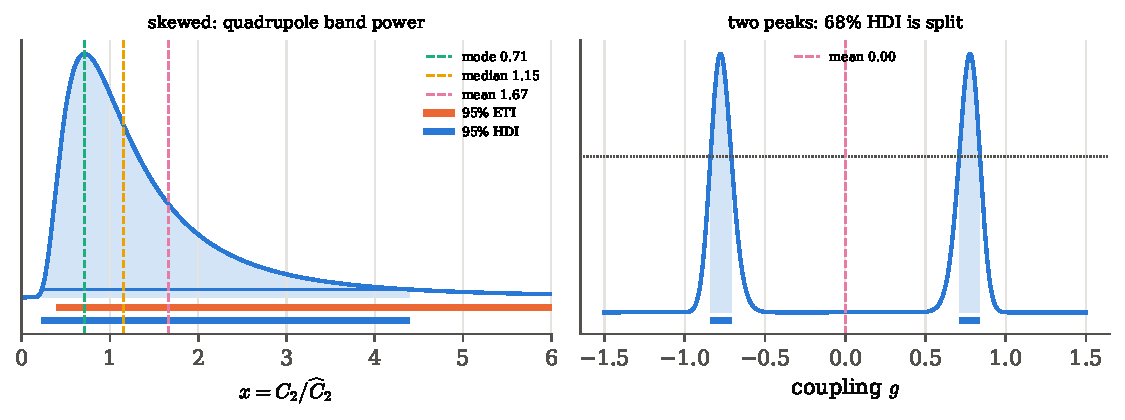
\includegraphics[width=\linewidth]{figures/ch05/summaries.pdf}
\caption{Summaries of two posteriors. Left: the skewed posterior of the quadrupole
power relative to its estimate, with its mode, median and mean (vertical dashed lines),
the 95\% equal-tailed interval (upper bar, orange) and the 95\% HDI (lower bar, blue,
shaded, with its water level). Right: the two-peaked coupling posterior. Its 68\% HDI is
two intervals, and its mean falls in the gap between the peaks.}
\label{5b:fig:summaries}
\end{figure}

\subsection{What a credible interval says, and what a confidence interval says}

A 95\% credible interval makes a direct statement about the parameter: given these data
and this prior, the probability that $\theta$ lies in the interval is 0.95. A 95\%
confidence interval (\cref{ch:03,ch:04}) makes a statement about a procedure: if the
experiment were repeated many times, intervals built this way would cover the fixed true
value in 95\% of the repetitions \srcref{Lambert}{\S7.7}. The two are different
statements and need not agree. Often, though, the numbers are the same. For a
Gaussian likelihood and a flat or broad prior the posterior is $\Normal(\bar\theta,\tau^2)$ with
$\bar\theta\approx\hat\theta$ and $\tau\approx\mathrm{se}$, where $\hat\theta$ is the
maximum-likelihood estimate and $\mathrm{se}$ its standard error. So the 95\% credible
interval $\bar\theta\pm1.96\tau$ is approximately the frequentist $\hat\theta\pm1.96\,
\mathrm{se}$ \mainref{p.~179}. For large samples this agreement is general
(\cref{5b:sec:laplace}). For small samples, skewed posteriors, parameters near a
physical boundary, or informative priors, they can differ substantially, and in high
dimensions a 95\% credible region need not cover the truth 95\% of the time
\mainref{p.~189}.

\begin{pitfall}[Credible is not confidence]
``The parameter lies in $[a,b]$ with 95\% probability'' is a correct reading of a
credible interval and an incorrect reading of a confidence interval. Conversely,
``this interval covers the truth in 95\% of repeated experiments'' is guaranteed for a
confidence interval and not, in general, for a credible interval. When a result is
quoted, say which kind it is, and for a credible interval say which prior was used and
whether it is an HDI or an equal-tailed interval.
\end{pitfall}
\section{The Gaussian approximation: a peak and its curvature}
\label{5b:sec:laplace}

Most posteriors in a mature experiment look like a single smooth bump. Then two numbers
describe the whole curve well: where the bump is and how wide it is. The result is
quoted as ``$\theta=\theta_0\pm\sigma$''. Where do these two numbers come from, in one
parameter and in many? And when does this description mislead?

\subsection{One parameter}

We work with the logarithm of the posterior, $L(\theta)=\ln p(\theta\given\data)$, for
two reasons. It turns products of likelihoods into sums. And near a peak it varies much
more gently than the posterior itself, so a short Taylor series describes it well
\srcref{Sivia}{(2.10)}. Let $\theta_0$ be the peak, so $L'(\theta_0)=0$ and
$L''(\theta_0)<0$, and Taylor-expand about it:
\begin{align}
  L(\theta)
  &\eqby{1}L(\theta_0)+L'(\theta_0)(\theta-\theta_0)
     +\tfrac12L''(\theta_0)(\theta-\theta_0)^2+\dots
   \nonumber\\
  &\eqby{2}L(\theta_0)-\frac{(\theta-\theta_0)^2}{2\sigma^2}+\dots,
   \qquad \sigma\equiv\bigl(-L''(\theta_0)\bigr)^{-1/2}.
  \label{5b:eq:laplace}
\end{align}
\begin{explain}
  \item Taylor's theorem to second order about $\theta_0$.
  \item The linear term vanishes at a maximum, and $L''(\theta_0)$ is negative, so we
        may write it as $-1/\sigma^2$.
\end{explain}
Exponentiate and drop the higher terms. The exponential of $-(\theta-\theta_0)^2/
2\sigma^2$ is a Gaussian, so $p(\theta\given\data)\approx\Normal(\theta_0,\sigma^2)$
\srcref{Sivia}{(2.13)--(2.15)}. This is the \newterm{Gaussian} or \newterm{Laplace
approximation}. In words: the error bar is one over the square root of the curvature of
the log-posterior at its peak. A sharply curved peak means a small error bar. Within the approximation, $\theta_0\pm\sigma$ holds 68\% of
the probability and $\theta_0\pm2\sigma$ holds 95\%.

\paragraph{Example: Gaussian readings.}
For $N$ readings of equal error $\sigma_x$ and a flat prior, $L=\text{const}-\sum_k(x_k-
\mu)^2/2\sigma_x^2$. Then $L'=\sum_k(x_k-\mu)/\sigma_x^2=0$ gives $\mu_0=\bar x$, and
$L''=-N/\sigma_x^2$ gives $\sigma=\sigma_x/\sqrt N$ \srcref{Sivia}{(2.28)--(2.29)}. Here
the expansion is exact, because $L$ is a quadratic and all higher derivatives vanish.

\paragraph{Example: the coin.}
With a flat prior and $R$ heads in $N$ tosses, $L=\text{const}+R\ln\theta+(N-R)\ln(1-
\theta)$ \srcref{Sivia}{(2.17)}. Then
\begin{align*}
  L'(\theta)&\eqby{1}\frac R\theta-\frac{N-R}{1-\theta}=0
  \;\Rightarrow\;\theta_0=\frac RN,\\
  L''(\theta_0)&\eqby{2}-\frac{R}{\theta_0^2}-\frac{N-R}{(1-\theta_0)^2}
  \eqby{3}-\frac{N}{\theta_0}-\frac{N}{1-\theta_0}
  \eqby{4}-\frac{N}{\theta_0(1-\theta_0)} ,
\end{align*}
\begin{explain}
  \item Differentiate the logs, and solve $R(1-\theta_0)=(N-R)\theta_0$.
  \item Differentiate once more.
  \item Substitute $R=N\theta_0$ and $N-R=N(1-\theta_0)$.
  \item Common denominator: $\frac{1}{\theta_0}+\frac{1}{1-\theta_0}=\frac{1}{\theta_0(1-\theta_0)}$.
\end{explain}
so $\sigma=\sqrt{\theta_0(1-\theta_0)/N}$ \srcref{Sivia}{(2.19)--(2.20)}, the familiar
binomial error. The width shrinks like $1/\sqrt N$. At fixed $N$ it is largest for
$\theta_0=\frac12$, so it is easier to show that a coin is strongly biased than to show
that it is fair.

How good is the approximation? It depends on the data. For 9 heads in 32 tosses it
gives $\theta=\FiveBLapHa\pm\FiveBLapSa$. The exact posterior is a Beta density
(\cref{5b:sec:conjugate}) with mean $\FiveBLapMeanA$ and standard deviation
$\FiveBLapSdA$, so the two agree well (\cref{5b:fig:laplace-coin}, left). For 1 head in
10 the approximation gives $\FiveBLapHb\pm\FiveBLapSb$. It puts $\FiveBLapNegB$ of its
probability at $\theta<0$, which is impossible. The exact posterior is squeezed against
the boundary $\theta=0$ and skewed, with mean $\FiveBLapMeanB$. So near a physical
boundary, and with few data, an error bar is the wrong summary: quote an interval from
the posterior itself (\cref{5b:sec:summaries}).

\begin{figure}[htbp]
\centering
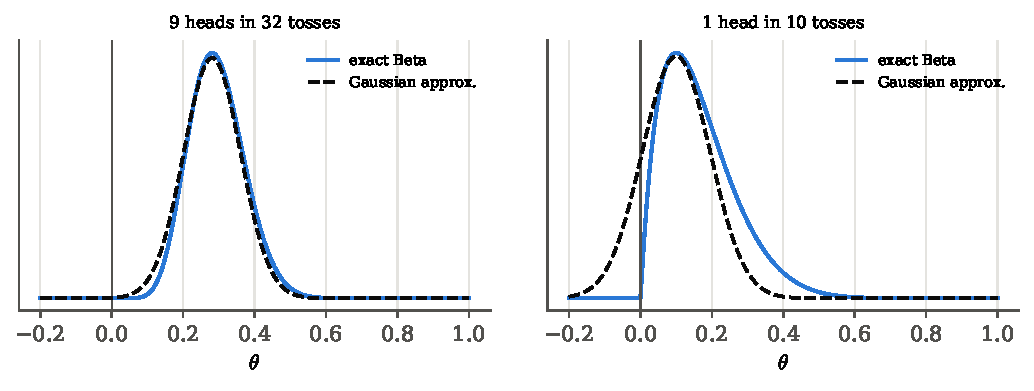
\includegraphics[width=0.92\linewidth]{figures/ch05/laplace_coin.pdf}
\caption{The Gaussian approximation (dashed) against the exact posterior (solid) for a
coin with a flat prior. Left: 9 heads in 32 tosses, where the two nearly agree. Right:
1 head in 10 tosses, where the exact posterior is pressed against the boundary
$\theta=0$ and the Gaussian spills probability into the impossible region to its left.}
\label{5b:fig:laplace-coin}
\end{figure}

\subsection{Several parameters: the Hessian and its inverse}

With parameters $\params=(\theta_1,\dots,\theta_M)$ the same expansion about the peak
$\params_0$ reads \srcref{Sivia}{(3.30)--(3.31)}
\begin{equation}
  L(\params)\approx L(\params_0)+\tfrac12(\params-\params_0)\T\mathbf H\,(\params-\params_0),
  \qquad H_{ij}=\left.\frac{\partial^2L}{\partial\theta_i\,\partial\theta_j}\right|_{\params_0},
  \label{5b:eq:hessian}
\end{equation}
where the linear term has again vanished because $\params_0$ is the peak. The matrix
$\mathbf H$ of second derivatives is the \newterm{Hessian}. Exponentiating, the
posterior is approximately a multivariate Gaussian with covariance matrix
$\Cmat=-\mathbf H^{-1}$ \srcref{Sivia}{(3.32)}, just as $\sigma^2=-1/L''$ in one
dimension. Its contours are ellipses (ellipsoids in more dimensions). Their axes point
along the eigenvectors of $\mathbf H$, and their lengths are proportional to
$|h_i|^{-1/2}$, where $h_i$ are the eigenvalues of $\mathbf H$ \srcref{Sivia}{Fig.~3.6}.
The peak really is a maximum only if all eigenvalues are negative.

\paragraph{Example: two parameters, done by hand.}
Write the second derivatives at the peak as $A=\partial_X^2L$, $B=\partial_Y^2L$,
$C=\partial_X\partial_YL$ \srcref{Sivia}{(3.19)}. A maximum needs $A<0$, $B<0$ and
$AB>C^2$. The inverse of a $2\times2$ matrix is
$\bigl(\begin{smallmatrix}A&C\\C&B\end{smallmatrix}\bigr)^{-1}
=\frac{1}{AB-C^2}\bigl(\begin{smallmatrix}B&-C\\-C&A\end{smallmatrix}\bigr)$, so
\begin{align}
  \Cmat=-\mathbf H^{-1}
  &\eqby{1}\frac{1}{C^2-AB}\begin{pmatrix}B&-C\\-C&A\end{pmatrix},
  \qquad
  \sigma_X^2\eqby{2}\frac{B}{C^2-AB},\quad
  \sigma_Y^2=\frac{A}{C^2-AB},\quad
  \sigma_{XY}\eqby{3}\frac{C}{AB-C^2}.
  \label{5b:eq:cov2}
\end{align}
\begin{explain}
  \item The $2\times2$ inverse, with the overall minus sign absorbed into the
        denominator.
  \item The diagonal entries are the variances. Both $B$ and $C^2-AB$ are negative,
        so $\sigma_X^2>0$ \srcref{Sivia}{(3.21)--(3.22)}.
  \item The off-diagonal entry is the covariance \srcref{Sivia}{(3.27)}.
\end{explain}
The correlation coefficient is $\rho=\sigma_{XY}/(\sigma_X\sigma_Y)=C/\sqrt{AB}$.

There are two different error bars for $X$, and they answer different questions. The
\newterm{marginal} error $\sigma_X$ of \eqref{5b:eq:cov2} answers: how far can $X$ move
if $Y$ may be anything the data permit (\cref{5b:sec:marginal})? The
\newterm{conditional} error answers: how far can $X$ move if $Y$ is held fixed at its
best value? With $Y$ fixed, only the curvature in $X$ matters, so
$\sigma_{X|Y}=(-A)^{-1/2}$. How much smaller is the second? Their ratio is
\begin{align*}
  \frac{\sigma_X^2}{\sigma_{X|Y}^2}
  \eqby{1}\frac{B}{C^2-AB}\,(-A)
  \eqby{2}\frac{AB}{AB-C^2}
  \eqby{3}\frac{1}{1-\rho^2}\;\ge1 .
\end{align*}
\begin{explain}
  \item Divide \eqref{5b:eq:cov2} by $1/(-A)$.
  \item Multiply numerator and denominator by $-1$.
  \item Divide numerator and denominator by $AB$ and use $\rho^2=C^2/(AB)$.
\end{explain}
So holding a correlated parameter fixed always makes the error bar look smaller, by a
factor $\sqrt{1-\rho^2}$. With $\rho=0.95$ the conditional error is a third of the honest
one \srcref{Sivia}{Fig.~3.8}. \Cref{5b:fig:ellipse} shows the geometry. The conditional
error is the width of a horizontal slice through the centre of the ellipse. The marginal
error is the width of the ellipse's shadow on the $X$ axis.

\begin{figure}[htbp]
\centering
\begin{tikzpicture}[x=1cm,y=1cm]
  \draw[faint,->] (-3.3,0) -- (3.4,0) node[right,black,lbl] {$X$};
  \draw[faint,->] (0,-2.3) -- (0,2.4) node[above,black,lbl] {$Y$};
  \draw[form,rotate=35] (0,0) ellipse (2.6 and 0.55);
  \draw[fibre,line width=2pt] (-0.918,0) -- (0.918,0);
  \draw[bdryred,dashed] (-2.153,-2.0) -- (-2.153,1.6);
  \draw[bdryred,dashed] (2.153,-1.6) -- (2.153,2.0);
  \draw[bdryred,very thick] (-2.153,-1.9) -- (2.153,-1.9);
  \node[lbl,bdryred,anchor=north] at (0,-1.95) {marginal: shadow on the $X$ axis};
  \node[lbl,fibreorange,align=center,anchor=north] at (1.35,-0.75) {conditional slice\\at $Y=Y_0$};
  \draw[fibreorange,thin] (1.0,-0.72) -- (0.55,-0.03);
\end{tikzpicture}
\caption{Conditional against marginal error for two correlated parameters. The ellipse
is a contour of the Gaussian posterior. Holding $Y$ at its best value and asking how
far $X$ may move gives the short orange slice, of half-width $(-A)^{-1/2}$. Letting $Y$
take any value gives the full shadow of the ellipse on the $X$ axis, between the red
dashed tangents, of half-width proportional to $\sqrt{B/(C^2-AB)}$.}
\label{5b:fig:ellipse}
\end{figure}

\begin{keyidea}[error bars from the curvature]
Near its peak, the log-posterior is a quadratic form with Hessian $\mathbf H$. The
posterior is then approximately Gaussian with covariance $\Cmat=-\mathbf H^{-1}$. The
honest (marginal) error bar on $\theta_i$ is $\sqrt{\Cmat_{ii}}=\sqrt{[(-\mathbf H)^{-1}]_{ii}}$,
the square root of a diagonal element of the \emph{inverse}. The inverse of a diagonal
element, $1/\sqrt{-H_{ii}}$, is the conditional error with all other parameters frozen,
and is always smaller or equal.
\end{keyidea}

\paragraph{The link to the Fisher matrix.}
The Laplace approximation and the Fisher forecast of \cref{ch:10} are the same object,
seen after and before the data are taken. Here is why. With a flat prior, $-\mathbf H$
is the curvature of the log-likelihood at its maximum, called the \emph{observed
information}. Average it over all the data sets the model could have produced, and we
get the \newterm{Fisher matrix} $\Fish$, with $F_{ij}=-\E[\partial_i\partial_j\ln
\Like]$. So $\Fish^{-1}$ is the expected posterior covariance. Then
$\sqrt{(\Fish^{-1})_{ii}}$ is the expected marginal error, and $1/\sqrt{F_{ii}}$ the
expected conditional one \srcref{Padilla}{\S3.8}.

For a Gaussian likelihood with a model linear in the parameters, $L$ is exactly
quadratic. The Hessian then does not depend on the parameters, and the approximation is
exact \srcref{Sivia}{\S3.4, (3.52)}. For nonlinear models the peak itself is usually
found step by step, by Newton--Raphson steps $\params_{k+1}=\params_k-\mathbf H^{-1}
\nabla L$ \srcref{Sivia}{(3.55)}, as in \cref{ch:03}.

\paragraph{Example: contours for two parameters.}
Which contour of a two-parameter posterior holds 68\% of the probability? Measure the
distance from the peak by $Q=(\params-\params_0)\T\Cmat^{-1}(\params-\params_0)$. Within
the Gaussian approximation, $Q=2[L(\params_0)-L(\params)]$, the ``$\Delta\chi^2$'' from
the peak. The contours are the curves $Q=k$, so we need the distribution of $Q$. Change
variables to $\bm u=\Cmat^{-1/2}(\params-\params_0)$. This turns the Gaussian into $M$
independent standard normals, so $Q=\sum_iu_i^2$ has a $\chi^2$ distribution with $M$
degrees of freedom (\cref{ch:02}). For $M=2$ that distribution is an exponential,
$p(Q)=\frac12e^{-Q/2}$, so
\begin{align*}
  \Prob(Q\le k)\eqby{1}\int_0^k\tfrac12e^{-Q/2}\dd Q\eqby{2}1-e^{-k/2}
  \\
  \Rightarrow\quad
  k_{68.3\%}=-2\ln(1-0.683)=2.30,\qquad k_{95.4\%}=6.17 .
\end{align*}
\begin{explain}
  \item The $\chi^2_2$ density is $\frac12e^{-Q/2}$.
  \item Elementary integral, then solve for $k$.
\end{explain}
These are the contour levels ``$\Delta\chi^2=2.30$ and $6.17$'' used in every
two-parameter plot in cosmology \srcref{Padilla}{Table~III}. In one dimension the same
argument gives $\Delta\chi^2=1$ and $4$ for $\pm1\sigma$ and $\pm2\sigma$: a one-parameter
interval and a two-parameter contour at the same confidence need different thresholds.

\subsection{When the approximation fails, and when it comes back: the lighthouse}

A lighthouse stands at unknown position $\alpha$ along a straight coast, a known
distance $\beta$ out to sea \srcref{Sivia}{\S2.4}. It emits short flashes in random
directions, uniformly in the azimuth $\vartheta\in(-\pi/2,\pi/2)$. Detectors along the
shore record \emph{where} each flash arrives, $x=\alpha+\beta\tan\vartheta$, but not its
direction (\cref{5b:fig:lighthouse-geom}). Where is the lighthouse?

\begin{figure}[htbp]
\centering
\begin{tikzpicture}[x=1cm,y=1cm]
  \fill[formblue!8] (-3.5,0) rectangle (4.5,2.4);
  \draw[thick] (-3.5,0) -- (4.5,0) node[right,lbl] {shore, $x$};
  \node[lbl,anchor=south west] at (-3.4,2.0) {sea};
  \fill (0,2) circle (2.2pt);
  \node[lbl,anchor=south east] at (-0.1,2.05) {lighthouse};
  \draw[faint,dashed] (0,2) -- (0,0);
  \node[lbl,anchor=east] at (-0.05,1.0) {$\beta$};
  \draw[->,thick,fibreorange] (0,2) -- (2.4,0);
  \draw[faint] (0,1.4) arc (-90:-50.2:0.6);
  \node[lbl,anchor=north west] at (0.25,1.35) {$\vartheta$};
  \fill (0,0) circle (1.5pt);
  \node[lbl,anchor=north] at (0,-0.08) {$\alpha$};
  \fill[fibreorange] (2.4,0) circle (1.5pt);
  \node[lbl,anchor=north] at (2.4,-0.08) {$x_k$};
\end{tikzpicture}
\caption{The lighthouse problem. A flash leaves at azimuth $\vartheta$, uniformly
distributed, and reaches the shore at $x_k=\alpha+\beta\tan\vartheta$. Only the arrival
point is recorded.}
\label{5b:fig:lighthouse-geom}
\end{figure}

The likelihood of one arrival point follows from the change of variables for densities
(\cref{ch:01}):
\begin{align*}
  p(x\given\alpha,\beta)
  \eqby{1}p(\vartheta)\left|\frac{\dd\vartheta}{\dd x}\right|
  \eqby{2}\frac1\pi\cdot\frac{1}{\beta\,(1+\tan^2\vartheta)}
  \eqby{3}\frac{\beta}{\pi\,[\beta^2+(x-\alpha)^2]} .
\end{align*}
\begin{explain}
  \item The probability in a small range $\dd\vartheta$ equals that in the matching
        $\dd x$.
  \item $p(\vartheta)=1/\pi$ on $(-\pi/2,\pi/2)$, and $\dd x/\dd\vartheta=\beta/\cos^2
        \vartheta=\beta(1+\tan^2\vartheta)$.
  \item $\tan\vartheta=(x-\alpha)/\beta$.
\end{explain}
This is a Cauchy (Lorentzian) density \srcref{Sivia}{(2.34)}, with a peak at $\alpha$ and
tails so heavy that its variance is infinite (\cref{ch:02}). Take a flat prior on
$\alpha$ and independent flashes at $x_1,\dots,x_N$. The log-posterior is
$L(\alpha)=\text{const}-\sum_k\ln[\beta^2+(x_k-\alpha)^2]$ \srcref{Sivia}{(2.38)}. The
condition $L'=0$ for its peak cannot be solved in closed form, but on a grid the whole
posterior is easy to compute.

\Cref{5b:fig:lighthouse} shows the posterior as flashes accumulate, for a lighthouse at
$\alpha=1$\,km with $\beta=1$\,km. After one or two flashes the posterior is broad with
heavy tails. When two flashes land far apart, the posterior has two humps, one near
each. In this run, by eight flashes it is a single bump. After 64 its standard deviation, $\FiveBLhSdSix$, agrees
with the Laplace width $\FiveBLhLapSix$ from the curvature at the peak. After 512 flashes the posterior is
$\alpha=\FiveBLhModeFive\pm\FiveBLhSdFive$\,km, and the width matches the large-$N$
prediction $\beta\sqrt{2/N}=\FiveBLhSqrtTwoN$\,km that follows from the Fisher
information of a Cauchy density.

The sample mean of the arrival points would be the answer for Gaussian data. Here it
does not converge at all: after 64 flashes it is $\FiveBLhXbarSix$, and on average it
is no closer to the truth than a single flash. Why? For Cauchy data the average of $N$ points has the same Cauchy
distribution as a single point, because the central limit theorem needs a finite
variance (\cref{ch:02}). One wild flash, sent almost parallel to the shore, can drag the
mean anywhere. The posterior never uses the mean. It weighs every flash through the
likelihood. A wild flash far from $\alpha$ has a likelihood that is nearly flat in
$\alpha$, so it barely moves the posterior \srcref{Sivia}{p.~36}.

\begin{figure}[htbp]
\centering
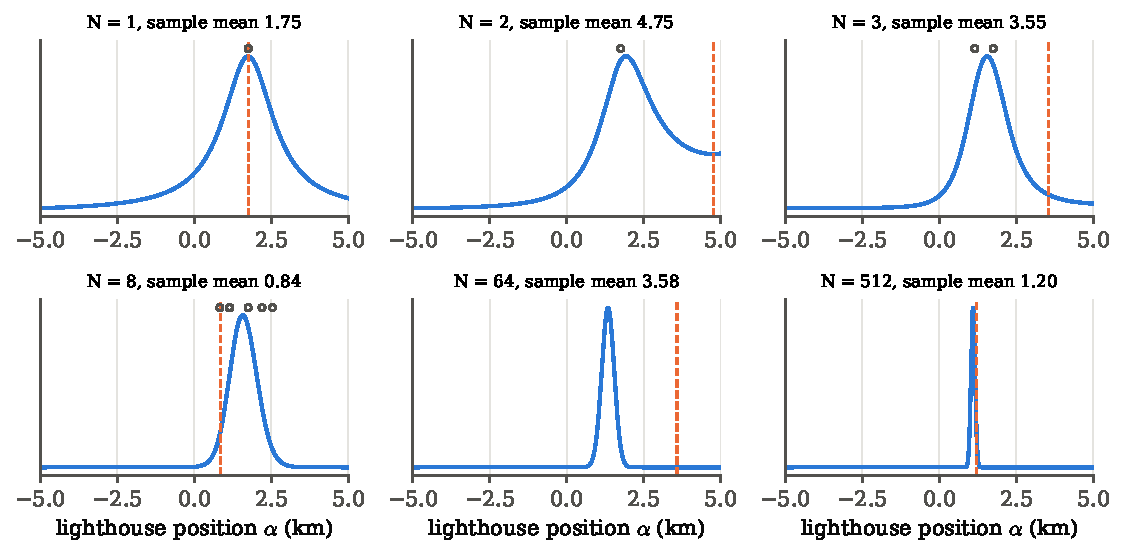
\includegraphics[width=\linewidth]{figures/ch05/lighthouse.pdf}
\caption{The posterior for the lighthouse position as flashes accumulate ($N$ in each
title). Circles at the top of the first four panels mark where the flashes landed, and
the dashed vertical line is the sample mean of the arrival points. The posterior starts
broad and sometimes two-peaked, becomes a narrow Gaussian-like peak near the true
$\alpha=1$\,km, while the sample mean keeps jumping around.}
\label{5b:fig:lighthouse}
\end{figure}

The lighthouse shows both sides of the Gaussian approximation. With few data the
posterior can be lopsided or have several peaks, and no ``$\theta_0\pm\sigma$''
describes it. With many data from a well-behaved likelihood the posterior becomes a
Gaussian of width $1/\sqrt{N\,I}$, where $I$ is the Fisher information of one datum,
whatever the shape of the single-datum likelihood. That second half is
a theorem, the Bernstein--von Mises theorem of \cref{5b:sec:bvm}.
\section{Nuisance parameters: integrating out what we do not care about}
\label{5b:sec:marginal}

A spectrum shows a peak sitting on a smooth background: a Bragg peak on diffuse
scattering, an emission line on a quasar's continuum, a resonance on the falling
background of a collider mass spectrum. We want the amplitude $A$ of the peak. The
background level $B$ is of no interest in itself, but it cannot be ignored, because the
counts we measure are the sum of both, and a higher background leaves room for a
smaller peak \srcref{Sivia}{\S3.1}. Such a parameter, needed by the model and irrelevant
to the question, is a \newterm{nuisance parameter}. How do we get a posterior for $A$
alone that honestly includes our ignorance of $B$?

\subsection{Marginalising: the sum rule applied to parameters}

Bayes' theorem gives the joint posterior $p(A,B\given\data)$, a density over pairs of
values. Our question is about $A$ alone: what is the probability that $A$ lies in some
small range, whatever $B$ is? That can happen in many ways, one for each value of $B$,
and the sum rule says to add up their probabilities. This is marginalisation
(\cref{ch:01}). A marginal distribution isolates the probability of a single variable,
here $A$, by averaging out the ``nuisance'' variables, here $B$, from the joint
distribution:
\begin{equation}
  p(A\given\data)=\int p(A,B\given\data)\,\dd B
  \label{5b:eq:marg}
\end{equation}
\srcref{Sivia}{(3.9)}, \mainref{p.~183, (11.9)}, \srcref{Padilla}{(38)}. In the tree
picture it is the sum over all branches of $B$ that lead to the same $A$. With more
nuisance parameters the integral runs over all of them. This is why the standard output
of a cosmological analysis is a set of marginal posteriors, of one or two parameters
out of dozens \srcref{HobsonBMC}{(2.6)}.

\begin{workdef}[marginal posterior]
For parameters of interest $\params$ and nuisance parameters $\bm\nu$, the
\newterm{marginal posterior} is $p(\params\given\data)=\int p(\params,\bm\nu\given\data)\,
\dd\bm\nu$ \unpack{the joint posterior summed over every value of the nuisance
parameters, each weighted by how credible it is}. \emph{Operationally:} on a grid, sum
the joint posterior along the nuisance axes. From samples of the joint posterior,
simply ignore the nuisance coordinates (\cref{5b:sec:sampling}).
\end{workdef}

How does not knowing $B$ change what we learn about $A$? To see it, split the integrand
with the product rule, $p(A,B\given\data)=p(A\given B,\data)\,p(B\given\data)$:
\begin{equation}
  p(A\given\data)=\int p(A\given B,\data)\;p(B\given\data)\,\dd B .
  \label{5b:eq:marg-mix}
\end{equation}
The marginal is an average of the conditional posteriors $p(A\given B,\data)$, one for
each assumed background, weighted by how credible that background is. Now suppose an
independent calibration fixed the background exactly at $b$. Then $p(B\given\data)=
\delta(B-b)$ and
\begin{align*}
  p(A\given\data)
  \eqby{1}\int p(A\given B,\data)\,\delta(B-b)\,\dd B
  \eqby{2}p(A\given b,\data),
\end{align*}
\begin{explain}
  \item The calibration puts all the probability for $B$ at $b$.
  \item The delta function picks out the integrand at $B=b$.
\end{explain}
So the conditional posterior is the special case in which the nuisance parameter is
known perfectly \srcref{Sivia}{p.~44}. An analysis that ``fixes'' a parameter at a
fiducial value is doing exactly this, without saying so: it gives that parameter a
delta-function prior \srcref{HobsonBMC}{p.~42}. Any spread in $p(B\given\data)$ mixes
conditionals centred at different places, so the marginal is broader.

\paragraph{Example: a peak on a background.}
Following Sivia, the expected count in channel $k$ is $D_k=n_0[A\,e^{-x_k^2/2w^2}+B]$,
a Gaussian peak of known width and position on a flat background, and the observed count
$N_k$ is Poisson with mean $D_k$ \srcref{Sivia}{(3.1)--(3.4)}. With independent channels
and a flat prior on $A,B\ge0$,
\begin{equation*}
  \ln p(A,B\given\{N_k\})=\text{const}+\sum_k\bigl[N_k\ln D_k-D_k\bigr]
\end{equation*}
\srcref{Sivia}{(3.8)}, the log of a product of Poisson probabilities with the factorials
dropped. Here $n_0$ sets the overall count level, $x_k$ is the position of channel $k$
measured from the peak, and $w$ is the peak width.

How much does not knowing $B$ cost? It depends on whether the data can tell the peak
from the background. \Cref{5b:fig:signal-bkg} shows two simulated set-ups, both with
$A=1$, $B=2$.
\begin{itemize}[itemsep=1pt,leftmargin=1.2em]
  \item \emph{Wide set-up} (top row): 15 channels spread well beyond the peak. The
        outer channels measure the background alone, so $A$ and $B$ are only moderately
        correlated, $\rho=\FiveBMaRhoWide$. The marginal error on $A$ is
        $\FiveBMaSigWide$, against $\FiveBMaSigCondWide$ if $B$ were known to be 2.
  \item \emph{Narrow set-up} (bottom row): 7 channels over a narrow range around the
        peak. No channel sees the background alone, so a little more background and a
        little less peak fit almost equally well. The correlation is
        $\rho=\FiveBMaRhoNarrow$, and the marginal error on $A$ grows to
        $\FiveBMaSigNarrow$, almost three times the conditional error
        $\FiveBMaSigCondNarrow$.
\end{itemize}
Both ratios agree with the factor $1/\sqrt{1-\rho^2}$ of \cref{5b:sec:laplace}. So when
the data cannot separate signal from background, a calibration of the background is
worth a lot. When they can, it adds little \srcref{Sivia}{p.~42}.

\begin{figure}[htbp]
\centering
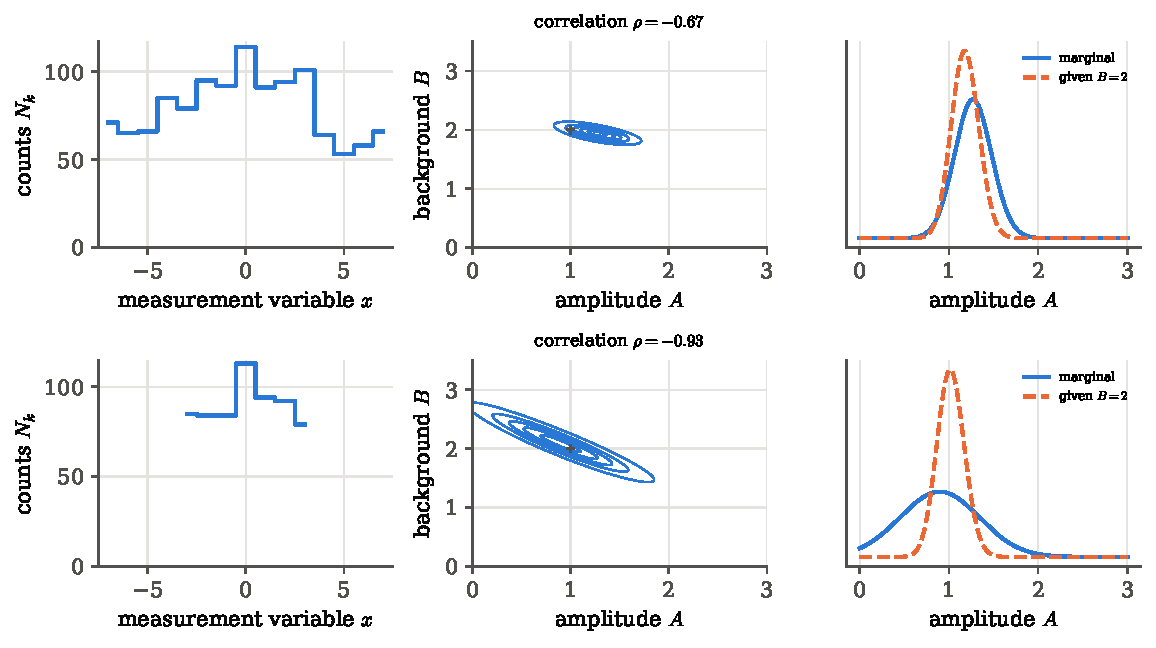
\includegraphics[width=\linewidth]{figures/ch05/marg_signal_bkg.pdf}
\caption{A peak of amplitude $A$ on a flat background $B$, from Poisson counts. Top:
15 channels spanning the peak and the background around it. Bottom: 7 channels
concentrated on the peak. Left: the simulated counts. Middle: contours of the joint
posterior at 10, 30, 50, 70 and 90\% of its maximum, with the true values marked by a
cross. Right: the marginal posterior of $A$ (solid) and the conditional posterior with
$B$ fixed at its true value (dashed). The narrow set-up correlates $A$ and $B$ strongly,
and marginalising over $B$ then widens the posterior of $A$ a lot.}
\label{5b:fig:signal-bkg}
\end{figure}

\paragraph{Example: an unknown noise level.}
Readings $x_k$ are Gaussian with mean $\mu$ and an error $\sigma$ that nobody told us.
Then $\sigma$ is a nuisance parameter, and \cref{ch:03} showed that integrating it out
with the prior $p(\sigma)\propto1/\sigma$ gives $p(\mu\given\data)\propto
\bigl[\sum_k(x_k-\mu)^2\bigr]^{-N/2}$ \srcref{Sivia}{(3.38)}, \srcref{HobsonBMC}{(2.26)}.
Its shape in $\mu$ follows from splitting the sum about the sample mean $\bar x$:
\begin{align*}
  \sum_k(x_k-\mu)^2
  &\eqby{1}\sum_k\bigl[(x_k-\bar x)+(\bar x-\mu)\bigr]^2\\
  &\eqby{2}\sum_k(x_k-\bar x)^2+2(\bar x-\mu)\sum_k(x_k-\bar x)+N(\bar x-\mu)^2
  \eqby{3}V+N(\bar x-\mu)^2,
\end{align*}
\begin{explain}
  \item Add and subtract $\bar x$ inside each square.
  \item Expand the square. The middle factor $(\bar x-\mu)$ does not depend on $k$.
  \item $\sum_k(x_k-\bar x)=0$ by the definition of $\bar x$, and $V\equiv\sum_k(x_k-\bar x)^2$.
\end{explain}
So $p(\mu\given\data)\propto[N(\bar x-\mu)^2+V]^{-N/2}$, a Student-$t$ curve centred on
$\bar x$ \srcref{Sivia}{(3.41)--(3.44)}. For large $N$ it approaches a Gaussian of width
$\sqrt{V/N^2}$, the familiar $s/\sqrt N$ with $s^2=V/N$. For small $N$ its tails are
much heavier than a Gaussian's. Not knowing the size of the noise costs precision, and
marginalisation builds that cost in automatically. (Sivia's flat prior on $\sigma$ gives the exponent
$-(N-1)/2$ instead, a slightly wider curve. The choice matters only for very few data.)

\subsection{Marginalising against profiling}

The frequentist way to remove a nuisance parameter is to \emph{maximise} over it: the
profile likelihood $\Like_p(A)=\max_B\Like(A,B)$ (\cref{ch:03}). Do integration and
maximisation agree?

For a Gaussian posterior they do. Write the log-posterior about its peak as
$L=\frac12(ax^2+2cxy+by^2)$ in the deviations $x=A-A_0$, $y=B-B_0$, with $a,b<0$ and
$ab>c^2$. Maximising over $y$ at fixed $x$ gives $by+cx=0$, so $y^\ast=-cx/b$, and
\begin{align*}
  L(x,y^\ast)
  \eqby{1}\tfrac12\Bigl(ax^2-\frac{2c^2x^2}{b}+\frac{c^2x^2}{b}\Bigr)
  \eqby{2}\tfrac12\,\frac{ab-c^2}{b}\,x^2 ,
  \qquad
  \int e^{L}\,\dd y
  \eqby{3}e^{\frac12\frac{ab-c^2}{b}x^2}\sqrt{\frac{2\pi}{-b}} .
\end{align*}
\begin{explain}
  \item Substitute $y^\ast=-cx/b$.
  \item Collect the terms over the common denominator $b$.
  \item Complete the square in $y$, $by^2+2cxy=b(y+cx/b)^2-c^2x^2/b$, and do the
        Gaussian integral over $y$. Its value $\sqrt{2\pi/(-b)}$ does not depend on $x$.
\end{explain}
Profile and marginal have the same $x$-dependence, so after normalisation they are the
same curve, with variance $b/(c^2-ab)$ as in \eqref{5b:eq:cov2}. The equality rests on
step (3): the width of the posterior in the nuisance direction, $(-b)^{-1/2}$, is the
same for every $x$.

When that width changes with the parameter of interest, the two disagree. To see by how
much, call the parameter of interest $\theta$ and the nuisance parameter $\nu$. At each
fixed $\theta$, expand $L$ about the best nuisance value $\hat\nu(\theta)$ and integrate
the Gaussian in $\nu$, exactly as in step (3). This gives
\begin{equation}
  p(\theta\given\data)=\int e^{L(\theta,\nu)}\,\dd\nu
  \;\approx\;\underbrace{e^{L(\theta,\hat\nu(\theta))}}_{\text{profile}}\;
  \underbrace{\sqrt{2\pi}\,\sigma_\nu(\theta)}_{\text{volume}},
  \qquad \sigma_\nu(\theta)=\bigl(-\partial_\nu^2L\bigr)^{-1/2}\big|_{\hat\nu(\theta)} .
  \label{5b:eq:volume}
\end{equation}
The first factor is the profile, the best fit at this $\theta$. The second measures how
many values of $\nu$ fit almost as well. So the marginal rewards values of $\theta$ for
which many values of the nuisance parameter fit the data, a large ``volume'' of good
fits. The profile only asks how good the best fit is.

\paragraph{Example: a weak bump of unknown position.}
Readings $y_i$ at 60 positions $x_i\in[0,10]$ follow $y_i=A\,e^{-(x_i-\mu)^2/2w^2}+
\epsilon_i$ with unit Gaussian noise and known narrow width $w=0.4$. A bump of true
amplitude $A=\FiveBVolAtrue$ sits at $\mu=5$, and we take flat priors on $A\in[0,4]$ and
on the position $\mu\in[0,10]$ (\cref{5b:fig:volume}). Here the amplitude $A$ is the
parameter of interest and the position $\mu$ the nuisance parameter.

How wide is the range of good positions? It depends on $A$. When $A$ is large, only
positions near the true bump fit, so the posterior in $\mu$ is narrow. When $A$ is near
zero, every position fits equally well, because a bump of zero height is invisible
wherever it is. Then the whole prior range of $\mu$ contributes. That large volume pulls
the marginal posterior of $A$ towards zero. For the data of \cref{5b:fig:volume} its
mode is at $A=\FiveBVolMargMode$, and it puts probability $\FiveBVolPsmallMarg$ on
$A<0.5$. The profile ignores volume. It peaks at $A=\FiveBVolProfMode$ and gives
$\FiveBVolPsmallProf$ to $A<0.5$. One data set could be a fluke, so we repeat the
analysis on $\FiveBVolLoopR$ fresh data sets with the same true bump. On average the
marginal gives $A<0.5$ a probability of $\FiveBVolLoopPsmallMarg$ and the profile
$\FiveBVolLoopPsmallProf$ (each to within about $\FiveBVolLoopErr$), and the marginal
peaks at $A=0$ in $\FiveBVolLoopModeZero$ of them.

Neither is wrong; they answer different questions. The profile says ``the best bump
anywhere has amplitude about $\FiveBVolProfMode$''. The marginal says ``averaged over
where a bump could be, small amplitudes are more credible than the best fit alone
suggests''.
This is the Bayesian face of the look-elsewhere effect (\cref{ch:04}). It is also a
first view of how the evidence penalises a model for its prior volume, the Occam factor
of model comparison.

\begin{figure}[htbp]
\centering
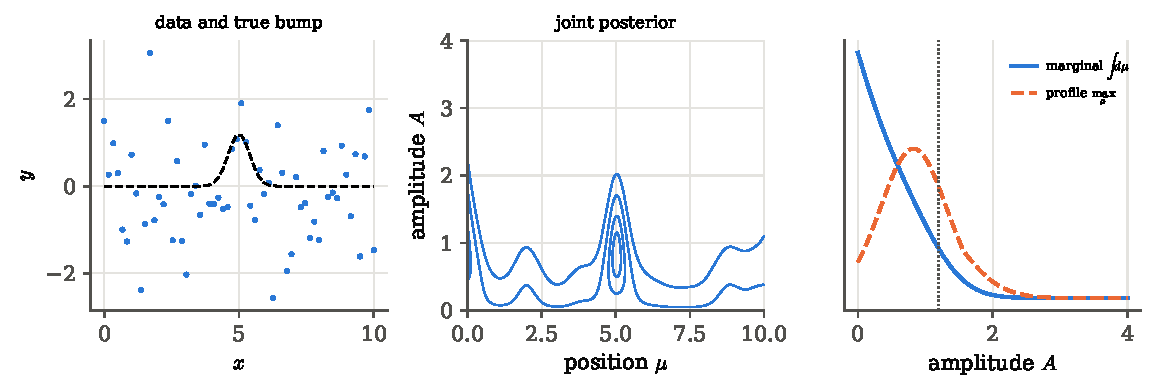
\includegraphics[width=\linewidth]{figures/ch05/marg_volume.pdf}
\caption{Marginal against profile for a weak bump whose position is unknown. Left: the
data and the true bump (dashed). Middle: the joint posterior of amplitude and position.
At small amplitude every position fits about equally well, so whatever probability the
posterior keeps there is spread over the whole range of positions. Right: the marginal
posterior of the amplitude (solid) integrates over position, so it gives small
amplitudes more weight than the profile (dashed), which maximises over position and
peaks near the best-fitting bump. The dotted line is the true amplitude.}
\label{5b:fig:volume}
\end{figure}

\begin{pitfall}[The peak of the joint is not the peak of the marginal]
The best-fit point of a joint posterior, projected onto one parameter, is the peak of
the profile, not of the marginal. For skewed or banana-shaped posteriors, and whenever
the nuisance width changes across the parameter of interest, the two differ, and quoting
``the best fit'' next to a marginal interval can put the best fit outside the interval.
In cosmology these ``projection'' or ``prior-volume'' effects are routine in analyses
with many nuisance parameters. Report which summary is quoted, and when they differ,
report both \srcref{Sivia}{p.~54}.
\end{pitfall}

Marginals also hide structure. Two strongly correlated parameters may each have a broad
marginal while their difference is sharply determined. And two pairs of parameters with
the same marginals can have very different joint posteriors
\srcref{Kruschke}{Fig.~12.1}. Whenever the question concerns a combination of parameters,
compute the posterior of that combination from the joint, not from the marginals. With
samples this is a one-line operation (\cref{5b:sec:sampling}).
\section{Choosing a prior: subjective, flat and Jeffreys}
\label{5b:sec:priors}

Every posterior so far has needed a prior density $p(\theta)$ for the parameter
$\theta$ we want, the weight each branch of the probability tree gets before the data
arrive. Sometimes the choice is easy: an earlier experiment measured the same quantity,
and its result is our prior. Often it is not. Suppose we are the first to measure the
fraction $\theta$ of cosmic-ray muons that fire a new trigger. We believe it lies
between 0 and 1 and not much more. What density should we write down, and how much
does the answer depend on that choice?

Two schools answer differently \mainref{pp.~181--182}. The first, called
\newterm{subjectivism}, says that the prior should reflect our opinion about $\theta$
before the data are collected. The second looks for a prior that expresses no opinion
at all, a ``noninformative'' prior. The obvious candidate is a flat prior,
$p(\theta)\propto\text{constant}$. Both are useful and both have traps. The trap of the
flat prior is the more surprising one. A prior cannot be flat in every way of describing
the same parameter, so ``flat'' always hides a choice of variable.

The questions, in words, are these.
\begin{enumerate}
  \item How do we turn real but vague knowledge into a density?
  \item What does a flat prior actually say, and when is a flat prior over an infinite
        range allowed?
  \item Is there a rule that gives the same answer whichever variable we use to
        describe the parameter?
\end{enumerate}

\subsection{Priors that encode knowledge}

A prior is a probability like any other. No probability, prior or likelihood, is ever
simply ``known''. Each one is an assignment that reflects the information $I$ we have.
We call $p(X\given I)$ a likelihood when $X$ is data, and a prior when $X$ is a
parameter and no new measurement is involved. The difference is one of name, not of
objectivity \srcref{Sivia}{\S5.5}. What makes an assignment objective is consistency:
two people with the same information should assign the same density. In practice there
are three routes from knowledge to a density, which we take in turn.

\paragraph{Informal assessment.} Think of ten points, each carrying 10\% of the prior
probability, and decide where they plausibly go \srcref{HobsonBMC}{\S1.3.2}. That gives
a rough centre, a rough width and a rough shape, which we then match to a standard
density. For a \emph{location} parameter \unpack{one that shifts the prediction, like a
peak position or a mass} with centre $c$ and width $w$, a Cauchy density
\begin{equation*}
  p(\theta)=\frac{w/\pi}{(\theta-c)^2+w^2}
\end{equation*}
is a good choice. Its heavy tails still give real weight to values far from the guess,
so the data can move the answer there if they demand it. For a positive \emph{intensity} \unpack{a rate or an
amplitude that cannot be negative} of plausible size $a$, an exponential
$p(\theta)=a^{-1}e^{-\theta/a}$, or a Gamma density if we also know a width, does the same
job \srcref{HobsonBMC}{(1.28)--(1.30)}. The prior does not have to be ``right'' in some
undefinable sense. It has to be reasonable.

\paragraph{Moment matching.} If earlier data exist, choose a standard density with the
same mean and standard deviation as those data \srcref{Lambert}{\S5.6.2}. For example,
five earlier determinations of a detector gain, with mean $1.02$ and scatter $0.05$,
give the prior $\Normal(1.02,0.05^2)$. Which moments to match is an arbitrary choice, so
this is a practical recipe rather than a principle.

\paragraph{Example: a prior elicited from quantiles.}
Experts find quantiles easier to state than standard deviations. Suppose a colleague
says: ``I would give even odds that the Hubble constant lies between 67 and
$73\,\mathrm{km\,s^{-1}Mpc^{-1}}$, and I think it is equally likely to be below 67 as
above 73.'' That is a statement of the 25\% and 75\% quantiles, $q_{25}=67$ and
$q_{75}=73$. For a Gaussian prior $\Normal(\mu,s^2)$ each quantile is $q=\mu+z\,s$, where
$z$ is the matching quantile of the standard normal, $z_{75}=-z_{25}=0.6745$
\srcref{Lambert}{\S5.6.3}. Then
\begin{align*}
  q_{75}-q_{25}&\eqby{1}(\mu+z_{75}s)-(\mu+z_{25}s)\eqby{2}2\times0.6745\,s
  &&\Rightarrow\quad s=\frac{73-67}{1.349}=4.45,\\
  q_{75}+q_{25}&\eqby{3}2\mu
  &&\Rightarrow\quad \mu=70 .
\end{align*}
\begin{explain}
  \item Each quantile of $\Normal(\mu,s^2)$ is $\mu$ plus the standard-normal quantile
        times $s$.
  \item $z_{25}=-z_{75}$ because the standard normal is symmetric.
  \item Adding instead of subtracting, the $z$ terms cancel for the same reason.
\end{explain}
So the elicited prior is $\Normal(70,4.45^2)$. With a panel of experts, the pairs
$(z,q)$ from all of them lie roughly on one straight line $q=\mu+zs$, and a linear
regression through them gives a pooled $\mu$ (the intercept) and $s$ (the slope).

\subsection{Flat priors, and flat priors over an infinite range}

A flat prior $p(\theta)=\text{constant}$ lets the likelihood alone set the shape of the
posterior, since $p(\theta\given\data)\propto\Like(\theta)\times\text{constant}$. For a
bounded parameter such as our trigger fraction, the constant is $1$ on $[0,1]$, and after
$z$ firings in $N$ muons the posterior is $\mathrm{Beta}(z+1,N-z+1)$ (\cref{5b:sec:conjugate}),
which seems very reasonable \mainref{p.~182}.

For a parameter with no natural bound, such as the mean $\theta$ of Gaussian readings,
a constant over the whole real line has infinite area. So it is not a probability
density at all. Such a prior is called \newterm{improper}. Can we use it anyway? We can
still multiply it by the likelihood, and then check whether the product can be
normalised.

\paragraph{Example: the mean of Gaussian readings with a flat improper prior.}
Take $n$ readings $x_1,\dots,x_n$, each $\Normal(\theta,\sigma^2)$ with known $\sigma$,
and $p(\theta)=c$ on the whole real line. Write $\bar x=\frac1n\sum_ix_i$. Then
\begin{align*}
  p(\theta\given x_1,\dots,x_n)
  &\relby{1}{\propto} c\prod_{i=1}^n e^{-(x_i-\theta)^2/2\sigma^2}
   \relby{2}{\propto}\exp\!\Bigl[-\frac{1}{2\sigma^2}\sum_{i=1}^n(x_i-\theta)^2\Bigr]\\
  &\eqby{3}\exp\!\Bigl[-\frac{1}{2\sigma^2}\sum_{i=1}^n(x_i-\bar x)^2\Bigr]
     \exp\!\Bigl[-\frac{n(\theta-\bar x)^2}{2\sigma^2}\Bigr]
   \relby{4}{\propto}\exp\!\Bigl[-\frac{(\theta-\bar x)^2}{2\sigma^2/n}\Bigr].
\end{align*}
\begin{explain}
  \item Posterior $\propto$ likelihood $\times$ prior, dropping the factors
        $1/\sqrt{2\pi\sigma^2}$ that do not contain $\theta$.
  \item The constant $c$ drops out, and a product of exponentials is the exponential of
        the sum.
  \item Write $x_i-\theta=(x_i-\bar x)+(\bar x-\theta)$ and square. The cross term is
        $2(\bar x-\theta)\sum_i(x_i-\bar x)=0$, because the deviations from the mean sum
        to zero.
  \item The first factor does not contain $\theta$.
\end{explain}
The posterior is $\Normal(\bar x,\sigma^2/n)$, a perfectly proper density, and its
95\% interval $\bar x\pm1.96\,\sigma/\sqrt n$ coincides exactly with the frequentist
confidence interval of \cref{ch:03} \mainref{p.~182}. An improper prior is harmless as
long as the posterior it produces is a well-defined probability distribution.

The safe way to think about an improper prior is as the limit of proper ones
\srcref{Sivia}{\S5.5}. Use a prior that is flat between bounds $A$ and $B$, compute the
posterior, and watch what happens as $A\to-\infty$ and $B\to\infty$. Usually the
posterior settles down and the bounds drop out, as they did above. If instead the
conclusions depend strongly on $A$ and $B$, the data carry very little information, and
the prior range, which is prior knowledge, is doing the work. Every maximum-likelihood or
least-squares fit uses this limit without saying so.

Improper priors are not harmless everywhere. Take the evidence $p(\data)=\int\Like\,p\,
\dd\theta$ of a model whose prior is flat over a width $W$, so $p=1/W$. The evidence
carries this factor $1/W$, so as $W\to\infty$ it goes to zero. The model then loses any
comparison with a model that knows even roughly what range to expect
\srcref{HobsonBMC}{\S1.3.2}. A flat prior
over an enormous range is also not ignorance. It says we are almost certain that
$|\theta|$ is enormous, since almost all of its area lies there. Are you really almost
certain that $|\theta|>10^{100}$?

\subsection{Flat in which variable?}

A flat prior is supposed to say ``we know nothing''. But knowing nothing about a
parameter should also mean knowing nothing about any other way of describing it. Can
one prior be flat in both? Return to the trigger fraction $p$ with the flat prior
$p\sim U(0,1)$, meant to represent our lack of information about $p$. A physicist might
equally describe the trigger by its log-odds
\begin{equation*}
  \psi=\ln\frac{p}{1-p},\qquad p=\frac{e^\psi}{1+e^\psi},
\end{equation*}
which runs over the whole real line. If we are ignorant about $p$, we are also ignorant
about $\psi$, so we should use a flat prior for $\psi$ too. But we have no freedom left:
the flat prior on $p$ already fixes the density of $\psi$. The rule is the change of
variables for densities (\cref{ch:01}): corresponding intervals must carry equal
probability, $p_\Psi(\psi)\,|\dd\psi|=p_P(p)\,|\dd p|$. So
\begin{align}
  p_\Psi(\psi)
  &\eqby{1}p_P\bigl(p(\psi)\bigr)\,\Bigl|\frac{\dd p}{\dd\psi}\Bigr|
   \eqby{2}1\times\frac{\dd}{\dd\psi}\frac{e^\psi}{1+e^\psi}
   \eqby{3}\frac{e^\psi(1+e^\psi)-e^\psi e^\psi}{(1+e^\psi)^2}
   \eqby{4}\frac{e^\psi}{(1+e^\psi)^2} .
  \label{5b:eq:logit-density}
\end{align}
\begin{explain}
  \item Change of variables for a density: equal probability in matching intervals.
  \item The flat density on $[0,1]$ is $1$, and $p(\psi)$ increases, so the absolute
        value is not needed.
  \item Quotient rule.
  \item The $e^{2\psi}$ terms cancel.
\end{explain}
This is a bump centred at $\psi=0$, not a flat line \mainref{p.~182}. How much of the
probability does the bump hold in $|\psi|<2$? That range corresponds to
$p\in(1/(1+e^2),\,e^2/(1+e^2))=(0.119,0.881)$, which the flat prior gives probability
$0.762$. So a flat prior on $p$ is a confident statement about $\psi$: the trigger is
probably neither extremely efficient nor extremely inefficient.

\Cref{5b:fig:logit-map} shows why. Equal steps in $p$ map onto steps in $\psi$ that are
narrow in the middle and wide at the ends. Each step carries the same probability, so
probability gets squeezed into the middle of the $\psi$ axis. The conclusion is
unavoidable: ``flat'' has no meaning until we say flat in which variable, because a flat
prior on a parameter is not flat on a nonlinear function of it. Flat priors are not
\newterm{transformation invariant}.

\begin{figure}[htbp]
\centering
\begin{tikzpicture}[x=7cm,y=0.55cm]
  \draw[->] (0,-4.4) -- (1.07,-4.4) node[right,lbl] {$p$};
  \draw[->] (0,-4.4) -- (0,4.7) node[above,lbl] {$\psi=\ln\frac{p}{1-p}$};
  \foreach \t in {0,0.5,1}{\draw (\t,-4.4) -- (\t,-4.6) node[below,lbl] {$\t$};}
  \foreach \s in {-4,-2,0,2,4}{\draw (0,\s) -- (-0.012,\s) node[left,lbl] {$\s$};}
  \draw[form,domain=0.013:0.987,samples=120] plot (\x,{ln(\x/(1-\x))});
  \foreach \t in {0.1,0.2,0.3,0.4,0.5,0.6,0.7,0.8,0.9}{
    \pgfmathsetmacro{\s}{ln(\t/(1-\t))}
    \draw[tangentgreen,thin] (\t,-4.4) -- (\t,\s);
    \draw[fibreorange,thin,dashed] (\t,\s) -- (0,\s);
    \fill[fibreorange] (0,\s) circle (1.3pt);
    \fill[formblue] (\t,\s) circle (1.1pt);
  }
  \node[lbl,align=center,anchor=north] at (0.5,-5.4) {equal steps of $0.1$ in $p$};
  \node[lbl,align=left,anchor=west] at (0.04,3.7) {each step in $p$ carries\\ prior probability $0.1$};
\end{tikzpicture}
\caption{Why a flat prior in $p$ is not flat in the log-odds $\psi$. The curve is
$\psi=\ln[p/(1-p)]$. Nine equally spaced values of $p$ (green lines) are carried up to
the curve and across to the $\psi$ axis (orange points). The orange points crowd
together near $\psi=0$ and spread apart towards the ends, so the same probability, $0.1$
per step, is packed densely in the middle of the $\psi$ axis and thinly at its ends:
the bump of \eqref{5b:eq:logit-density}.}
\label{5b:fig:logit-map}
\end{figure}

The same happens for any nonlinear function. Lambert's example is the probability
$u=\theta^2$ that two randomly chosen individuals both carry a disease of prevalence
$\theta$ \srcref{Lambert}{\S5.6.1}. A flat prior on $\theta\in[0,1]$ gives $u$ the
density $p(u)=p(\theta)\,|\dd\theta/\dd u|=1/(2\sqrt u)$, which piles up at $u=0$. For
ten individuals, $v=\theta^{10}$, the pile-up is sharper still,
$p(v)=\frac1{10}v^{-9/10}$. So a prior that looks uninformative about one quantity is
quite informative about others. This is why ``vague'' or ``diffuse'' are better words
than ``uninformative''.

\paragraph{Example: a scale parameter over four decades.}
The effect is largest for a positive \emph{scale} parameter \unpack{one that sets a
size, like a width, a lifetime or a noise level} whose order of magnitude is unknown.
Let $\lambda$ lie anywhere between $0.01$ and $100$, four decades. A prior flat in
$\lambda$ gives the decade $[10,100]$ the probability $(100-10)/(100-0.01)=
\FiveBPrFlatTop$, and the decade $[0.01,0.1]$ only $\FiveBPrFlatBottom$. So ``complete
ignorance'' has become a 90\% bet that $\lambda$ is in the top decade. A prior flat in $\ln\lambda$ instead gives each of the
four decades probability $\FiveBPrLogDecade$ (\cref{5b:fig:priors-param}, middle). For a
quantity whose order of magnitude is unknown, the second is clearly what we mean.

\paragraph{Why flat in $\ln\lambda$ is special.} A consistency argument makes this
precise \srcref{Sivia}{\S5.1}. The question is: what density says only ``this is a
location'' or only ``this is a scale''? Start with a location parameter $X$. If that is
all we know, then moving the origin by $x_0$ cannot change our density:
$p(X)\,\dd X=p(X+x_0)\,\dd(X+x_0)$ for every $x_0$. Since $\dd(X+x_0)=\dd X$, this says
$p(X)=p(X+x_0)$, so $p$ is constant: complete ignorance about a location is a uniform
density. If all we know about a length $L$ is that it is a scale, then changing the
units by a factor $\beta$ (nanometres to \aa ngstr\"oms) cannot change our density:
\begin{align*}
  p(L)\,\dd L=p(\beta L)\,\dd(\beta L)
  \;&\relby{1}{\Rightarrow}\; p(L)=\beta\,p(\beta L)\quad\text{for all }\beta>0\\
  &\relby{2}{\Rightarrow}\; p(\beta)=\frac{p(1)}{\beta}
  \;\relby{3}{\Rightarrow}\; p(L)\propto\frac1L .
\end{align*}
\begin{explain}
  \item $\dd(\beta L)=\beta\,\dd L$ for a constant $\beta$. Divide by $\dd L$.
  \item Set $L=1$ and solve for $p(\beta)$.
  \item Rename $\beta$ as $L$: the relation holds for every positive value.
\end{explain}
This is \newterm{Jeffreys' prior} for a scale parameter \srcref{Sivia}{(5.17)--(5.18)}.
In terms of $s=\ln L$ it is $p(s)=p(L)\,\dd L/\dd s=(1/L)\times L=\text{constant}$: flat
in the logarithm, which is why problems involving magnitudes are best done on
logarithmic graph paper. It is improper on $(0,\infty)$, so we use it between bounds
or check that the posterior is normalisable. It is also the prior
$p(\Cell)\propto1/\Cell$ used for a power-spectrum amplitude in \cref{5b:sec:conjugate}.

\subsection{Jeffreys' rule: a prior that does not depend on the coordinates}

Is there a recipe that gives the same prior whichever variable we choose, so that
``Jeffreys in $\theta$'' transformed to $\psi$ equals ``Jeffreys computed in $\psi$''?
Jeffreys found one \mainref{pp.~182--183}.

\begin{workdef}[Jeffreys' prior]
For a model with density $f(x\given\theta)$ for one datum, \newterm{Jeffreys' prior}
is $p(\theta)\propto\sqrt{I(\theta)}$, where $I(\theta)=-\E_\theta\bigl[\partial_\theta^2
\ln f(X\given\theta)\bigr]$ is the Fisher information \unpack{how sharply one datum pins
down $\theta$ on average, \cref{ch:03}}. For several parameters,
$p(\params)\propto\sqrt{\det I(\params)}$ with the Fisher information matrix.
\emph{Operationally:} compute the expected curvature of $\ln f$, take its square root,
and normalise if the result has finite area.
\end{workdef}

Why is it invariant? Let $\psi=h(\theta)$ be any smooth, one-to-one reparametrisation.
Use the equivalent form $I(\theta)=\E_\theta[(\partial_\theta\ln f)^2]$ of the Fisher
information from \cref{ch:03}. Then
\begin{align*}
  I_\psi(\psi)
  &\eqby{1}\E\Bigl[\Bigl(\frac{\partial\ln f}{\partial\psi}\Bigr)^2\Bigr]
   \eqby{2}\E\Bigl[\Bigl(\frac{\partial\ln f}{\partial\theta}\Bigr)^2\Bigr]
     \Bigl(\frac{\dd\theta}{\dd\psi}\Bigr)^2
   \eqby{3}I_\theta(\theta)\Bigl(\frac{\dd\theta}{\dd\psi}\Bigr)^2,
  \\
  \sqrt{I_\psi(\psi)}
  &\eqby{4}\sqrt{I_\theta(\theta)}\,\Bigl|\frac{\dd\theta}{\dd\psi}\Bigr| .
\end{align*}
\begin{explain}
  \item Fisher information in the new variable, as the mean square of the score.
  \item Chain rule, $\partial_\psi=(\dd\theta/\dd\psi)\,\partial_\theta$. The factor is
        not random and comes out of the expectation.
  \item The definition of $I_\theta$.
  \item Square root of both sides.
\end{explain}
The last line is exactly the change-of-variables law for a density,
$p_\psi(\psi)=p_\theta(\theta)\,|\dd\theta/\dd\psi|$. So the square root of the Fisher
information transforms as a density must. Computing Jeffreys' prior in $\theta$ and
transforming it to $\psi$ gives the same density as computing it in $\psi$ directly. Geometrically, $I$ is a metric on parameter space
\unpack{it measures how distinguishable nearby parameter values are by their data}, and
$\sqrt{\det I}$ is its volume element. Jeffreys' prior spreads prior mass uniformly
over distinguishable models, not over coordinate intervals
\srcref{HobsonBMC}{(1.47)--(1.54)}.

\paragraph{Example: the Bernoulli trigger.} One muon fires the trigger, $x=1$, with
probability $p$, or not, $x=0$. Then $\ln f=x\ln p+(1-x)\ln(1-p)$ and
\begin{align*}
  I(p)
  &\eqby{1}-\E\Bigl[-\frac{X}{p^2}-\frac{1-X}{(1-p)^2}\Bigr]
   \eqby{2}\frac{p}{p^2}+\frac{1-p}{(1-p)^2}
   \eqby{3}\frac1p+\frac1{1-p}
   =\frac{1}{p(1-p)} .
\end{align*}
\begin{explain}
  \item Differentiate $\ln f$ twice in $p$.
  \item $\E[X]=p$ and $\E[1-X]=1-p$.
  \item Cancel. Adding the fractions gives $1/[p(1-p)]$.
\end{explain}
Jeffreys' prior is $\sqrt{I(p)}=p^{-1/2}(1-p)^{-1/2}$, the
$\mathrm{Beta}(\tfrac12,\tfrac12)$ density \mainref{p.~183, Ex.~11.6}. It is not flat;
it rises at both ends. Compare it with the two other popular choices. The flat prior in
$p$ is $p^0(1-p)^0$. The prior flat in $\psi$ is the improper Haldane prior
$\mathrm{Beta}(0,0)\propto p^{-1}(1-p)^{-1}$. It is flat in $\psi$ because its density
in $\psi$ is $p^{-1}(1-p)^{-1}\times\dd p/\dd\psi=p^{-1}(1-p)^{-1}\times p(1-p)=1$, using
$\dd p/\dd\psi=p(1-p)$ from \eqref{5b:eq:logit-density}. Jeffreys' exponents,
$-\tfrac12$, lie halfway between the flat prior's $0$ and Haldane's $-1$.

\paragraph{Example: a Poisson rate and a Gaussian width.} Take a count $n$ with mean
$\lambda T$, where $\lambda$ is the rate and $T$ the exposure. Then $\ln f=n\ln\lambda-
\lambda T+\text{const}$, so $\partial_\lambda^2\ln f=-n/\lambda^2$ and
$I=\E[n]/\lambda^2=T/\lambda$. Jeffreys' prior is therefore $\lambda^{-1/2}$. With zero
observed events the posterior is $\propto\lambda^{-1/2}e^{-\lambda T}$, a
$\mathrm{Gamma}(\tfrac12,T)$ density. For this density $2T\lambda$ has the $\chi^2$
distribution with one degree of freedom, whose 95\% point is $3.84$. So the 95\% upper
limit is $\lambda<3.84/(2T)=1.92/T$, against $3.00/T$ from the flat prior
(\cref{5b:sec:conjugate}). Now take the width $\sigma$ of Gaussian noise. Then $\ln f=-\ln\sigma-(x-\mu)^2/2\sigma^2$, so
$\partial_\sigma^2\ln f=1/\sigma^2-3(x-\mu)^2/\sigma^4$, whose expectation is
$1/\sigma^2-3/\sigma^2=-2/\sigma^2$. So $I=2/\sigma^2$ and Jeffreys' prior is
$1/\sigma$, the scale prior found above from units alone.

\paragraph{Does it matter? The three priors on real numbers.}
\Cref{5b:fig:priors-param} and \cref{5b:lst:priors} compare the flat $\mathrm{Beta}(1,1)$,
Jeffreys $\mathrm{Beta}(\tfrac12,\tfrac12)$ and Haldane $\mathrm{Beta}(0,0)$ priors for
the trigger. With $1$ firing in $10$ muons the posterior means are $\FiveBPrFlatMeanTen$,
$\FiveBPrJefMeanTen$ and $\FiveBPrHalMeanTen$, and the 95\% upper limits are
$\FiveBPrFlatUpTen$, $\FiveBPrJefUpTen$ and $\FiveBPrHalUpTen$. With so little data, the
choice among ``noninformative'' priors changes the answer by a third. With $100$ firings in
$1000$ muons the means are $\FiveBPrFlatMeanThou$, $\FiveBPrJefMeanThou$ and
$\FiveBPrHalMeanThou$ and the upper limits $\FiveBPrFlatUpThou$, $\FiveBPrJefUpThou$ and
$\FiveBPrHalUpThou$: the choice has become irrelevant. A large sample makes the prior
irrelevant for a reason, and the same reason tells us when it fails (\cref{5b:sec:bvm}).

\pyfile[firstline=30,lastline=58,firstnumber=30,label={5b:lst:priors}]{code/ch05/14_priors.py}{Flat in which
variable: a flat prior seen in the log-odds, mass per decade for a scale parameter, and
three ``noninformative'' priors on the same data}

Lines~31--32 draw $10^5$ values of $p$ from the flat prior and transform each to its
log-odds. This is the change of variables done by sampling, and line~35 overlays the
exact density \eqref{5b:eq:logit-density}. Line~38 counts the fraction with $|\psi|<2$,
$\FiveBPrFracCentral$, against the exact $0.762$. Lines~41--44 compute the prior mass per
decade on $[0.01,100]$ for the two priors: for the flat prior it is the width of the
decade over the width of the range, and for the log-flat prior the log-width over the
log-width of the range. Lines~55--58 update each of the three Beta priors with the
conjugate rule $\mathrm{Beta}(a+z,b+N-z)$ of \cref{5b:sec:conjugate} and read off the
posterior mean and the 95\% quantile.

\begin{figure}[htbp]
\centering
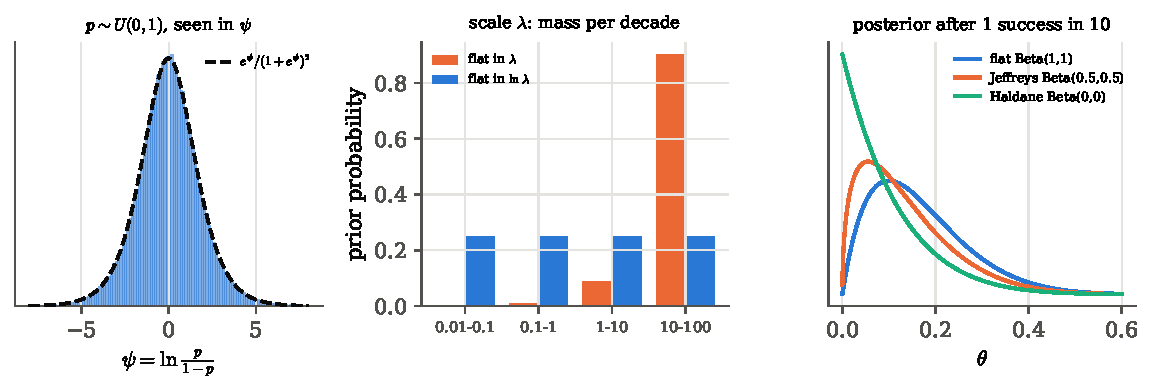
\includegraphics[width=\linewidth]{figures/ch05/priors_param.pdf}
\caption{Flat depends on the variable. Left: $10^5$ draws from a flat prior on $p$,
histogrammed in the log-odds $\psi$, follow the bump $e^\psi/(1+e^\psi)^2$ (dashed).
Middle: the prior probability of each decade of a scale parameter between $0.01$ and
$100$. Flat in $\lambda$ puts 90\% in the top decade. Flat in $\ln\lambda$ gives each
decade a quarter. Right: posteriors for a trigger efficiency after 1 firing in 10
muons, from the flat, Jeffreys and Haldane priors. With so few data they differ
visibly.}
\label{5b:fig:priors-param}
\end{figure}

\begin{pitfall}[There is no prior that says nothing]
Every prior says something about some function of the parameter. Jeffreys' rule is
consistent across coordinates, but it depends on the likelihood, so it changes when
the experiment changes, and in several dimensions $\sqrt{\det I}$ can behave badly or
fail to normalise \srcref{HobsonBMC}{\S1.3.2}. The general need for informal assessment
means that the search for a universal ``objective'' prior is doomed. Choose a
reasonable prior, say why, and check how much the answer depends on it
\srcref{Lambert}{\S5.7}.
\end{pitfall}

In practice most analyses use what Gelman calls \newterm{weakly informative} priors
\srcref{Lambert}{\S5.6.1}: smooth, proper densities that give zero weight only to
impossible values (a negative rate, a lifetime longer than the age of the universe) and
spread the rest broadly over physically sensible values. They avoid the arbitrary hard
edges of a flat box, which produce kinked posteriors and can trap the answer on the
wrong side of the edge (\cref{5b:sec:bvm}).
\section{Forgetting the prior: when the data win and when they cannot}
\label{5b:sec:bvm}

Two physicists measure the same trigger efficiency $\theta$, the fraction of muons that
fire a new trigger, with true value $0.3$. The first has no opinion and uses the flat
prior $\mathrm{Beta}(1,1)$. The second remembers a similar trigger with efficiency near
$0.8$ and is confident: $\mathrm{Beta}(80,20)$, a prior worth $\kappa=a+b=100$ muons
(\cref{5b:sec:conjugate}). Their priors barely overlap. They then record the same muons.
After ten muons they still disagree. After a hundred thousand they agree to a fraction of
an error bar (\cref{5b:fig:bvm-converge}). Is this agreement guaranteed? How fast does it
come? And when does it never come, however much data we take?

A second kind of forgetting is easy to confuse with this one. A Markov chain Monte
Carlo sampler (\cref{ch:09}) started at a silly point forgets where it started. That is
a different mechanism with a different cure. Keeping the two apart matters every time
someone says ``the prior washes out''.

\subsection{Why the prior is forgotten}

Write the log-posterior for $N$ independent data $x_1,\dots,x_N$ as
\begin{equation}
  \ln p(\theta\given x_1,\dots,x_N)
  =\underbrace{\ln p(\theta)}_{\text{one term}}
   +\underbrace{\sum_{i=1}^N\ln f(x_i\given\theta)}_{N\text{ terms}}
   +\text{const}.
  \label{5b:eq:logpost-N}
\end{equation}
Here $f(x\given\theta)$ is the density of one datum. The prior is a single term that
does not grow with $N$. The log-likelihood $\ell_N(\theta)=\sum_i\ln f(x_i\given\theta)$
is a sum of $N$ terms, so it grows in proportion to $N$. As data accumulate, the
likelihood therefore becomes a tall, narrow spike. The prior varies slowly across that
spike, so it can only nudge it. How much? Expand both terms about the
maximum-likelihood estimate $\hat\theta$, the peak of $\ell_N$. The curvature of $\ell_N$
there is $N\hat I$, where $\hat I=-\ell_N''(\hat\theta)/N$ is the observed information per
datum, close to the Fisher information $I(\theta)$ for large $N$ (\cref{ch:03}). Write
$g=\frac{\dd}{\dd\theta}\ln p(\theta)\big|_{\hat\theta}$ for the slope of the log-prior
there. Then
\begin{align}
  \ln p(\theta\given x_1,\dots,x_N)
  &\relby{1}{\approx}\text{const}+g\,(\theta-\hat\theta)
      -\frac{N\hat I}{2}(\theta-\hat\theta)^2
   \nonumber\\
  &\eqby{2}\text{const}'-\frac{N\hat I}{2}
      \Bigl(\theta-\hat\theta-\frac{g}{N\hat I}\Bigr)^2 .
  \label{5b:eq:bvm-shift}
\end{align}
\begin{explain}
  \item Taylor expansion about $\hat\theta$: the log-likelihood to second order (its
        first derivative vanishes at its peak), the log-prior to first order (it changes
        little across the narrow likelihood peak).
  \item Complete the square: $-\frac{c}{2}u^2+gu=-\frac c2(u-g/c)^2+g^2/2c$ with
        $u=\theta-\hat\theta$ and $c=N\hat I$. The $g^2/2c$ goes into the constant.
\end{explain}
The posterior is approximately Gaussian with
\begin{equation}
  \text{mean }\;\hat\theta+\frac{g}{N\hat I},\qquad
  \text{width }\;\frac{1}{\sqrt{N\hat I}},\qquad
  \frac{\text{shift caused by the prior}}{\text{width}}=\frac{g}{\sqrt{N\hat I}} .
  \label{5b:eq:bvm-ratio}
\end{equation}
The prior moves the posterior by an amount that falls as $1/N$. The posterior width
falls only as $1/\sqrt N$. So, measured in error bars, the influence of any smooth prior
dies away as $N^{-1/2}$. Two analysts with log-prior slopes $g_1$ and $g_2$ at
$\hat\theta$ disagree by $|g_1-g_2|/\sqrt{N\hat I}$ posterior standard deviations.

\begin{keyidea}[Bernstein--von Mises]
If the model is regular, the parameter is identifiable and of fixed dimension, and the
prior is smooth and nonzero at the true value, then for large $N$ the posterior is
approximately $\Normal\bigl(\hat\theta,\,1/[N I(\hat\theta)]\bigr)$, whatever the
prior. The posterior mean approaches the maximum-likelihood estimate, and a 95\%
credible interval approaches the 95\% confidence interval $\hat\theta\pm1.96/\sqrt{N
I(\hat\theta)}$ \mainref{p.~181, Thm.~11.5}.
\end{keyidea}

This is the Gaussian approximation of \cref{5b:sec:laplace} with a promise attached:
for large $N$ the curvature comes from the likelihood alone, so every reasonable prior
gives the same answer. This is why frequentist and Bayesian error bars on well-measured
quantities agree.

\paragraph{Example: two observers with Gaussian priors.}
Observers A and B have priors $\Normal(\mu_A,\Sigma_A^2)$ and $\Normal(\mu_B,\Sigma_B^2)$
for a quantity $\theta$ and share $N$ readings with Gaussian noise $\sigma$ and mean
$\bar m$ \srcref{Padilla}{\S3.4}. The rule ``precisions add'' of \cref{5b:sec:conjugate}
gives each observer $i\in\{A,B\}$ a Gaussian posterior with
\begin{align*}
  \hat\mu_i
  &\eqby{1}\frac{N\bar m/\sigma^2+\mu_i/\Sigma_i^2}{N/\sigma^2+1/\Sigma_i^2}
   \eqby{2}\frac{\bar m+r_i\,\mu_i}{1+r_i},
  \qquad r_i\equiv\frac{\sigma^2/N}{\Sigma_i^2},\\
  \tau_i^2
  &\eqby{3}\frac{1}{N/\sigma^2+1/\Sigma_i^2}
   \eqby{4}\frac{\sigma^2/N}{1+r_i}.
\end{align*}
\begin{explain}
  \item Precision-weighted mean \eqref{5b:eq:normal-post}: the $N$ readings count as
        one measurement $\bar m$ with variance $\sigma^2/N$.
  \item Divide numerator and denominator by $N/\sigma^2$.
  \item The posterior precision is the sum of the two precisions.
  \item Same division.
\end{explain}
The ratio $r_i$ compares the error of the data, $\sigma/\sqrt N$, with the width of the
prior, $\Sigma_i$. When $r_i\ll1$, the data dominate and $\hat\mu_i\to\bar m$ for both
observers. How fast do they converge? Since $r_i\propto1/N$, the difference
$\hat\mu_A-\hat\mu_B\approx r_A\mu_A-r_B\mu_B-(r_A-r_B)\bar m$ falls as $1/N$. The common
width $\tau\approx\sigma/\sqrt N$ falls only as $1/\sqrt N$. Their ratio falls as
$N^{-1/2}$, the law of \eqref{5b:eq:bvm-ratio} again. With one reading the two
posteriors can be far apart. After a hundred they are practically indistinguishable
\srcref{Padilla}{Fig.~3}.

\paragraph{Example: the confident and the open-minded physicist.}
Return to the two physicists of the opening: true efficiency $0.3$, a flat prior, and a
confident prior $\mathrm{Beta}(80,20)$. For the trigger the conjugate update is exact,
so we can follow the whole approach to agreement, not only its end. With $z$ firings in
$N$ muons and prior $\mathrm{Beta}(a,b)$ of mean $m_0=a/\kappa$, the posterior mean is
\begin{equation*}
  \frac{a+z}{\kappa+N}=\frac{N\hat\theta+\kappa m_0}{N+\kappa}
  \quad\Rightarrow\quad
  \text{mean}-\hat\theta=\frac{\kappa\,(m_0-\hat\theta)}{N+\kappa},
\end{equation*}
with $\hat\theta=z/N$. For the confident prior, $\kappa(m_0-\hat\theta)\approx100\times
(0.8-0.3)=50$. The flat prior's own pull, $2(0.5-\hat\theta)/(N+2)$, is tiny by
comparison. Dividing by the posterior width $\sqrt{\hat\theta(1-\hat\theta)/N}\approx
0.458/\sqrt N$ gives the gap between the two analysts in units of the posterior width,
\begin{equation*}
  \frac{\text{gap}}{\text{width}}\approx\frac{50}{N+100}\cdot\frac{\sqrt N}{0.458}
  =\frac{109\sqrt N}{N+100}.
\end{equation*}
Surprisingly, this \emph{grows} at first, because the posteriors narrow faster than
they approach each other. It peaks at $N=\kappa=100$, at about $5.5$ widths. That is the
moment of greatest embarrassment: both analysts are confident, and they disagree. Then
the gap falls as $109/\sqrt N$, the $N^{-1/2}$ law, and drops below one width only when
$N\gtrsim1.2\times10^4$. The simulation in \cref{5b:fig:bvm-converge} follows this curve:
its gap peaks at $\FiveBBvmGapPeak$ widths near $N=\FiveBBvmNpeak$ and stays below one
width from $N=\FiveBBvmNone$ on.

The lesson: a prior worth $\kappa$ observations needs many times $\kappa$ observations to
be forgotten. For a prior centred far from the truth, how many times is set by how many
widths away its centre lies. This matches Sivia's finding that a fair-minded coin prior
needs about a thousand flips before the data overrule it \srcref{Sivia}{\S2.1}, and
Lambert's that a strong model is less sensitive to the prior \srcref{Lambert}{\S5.7}.

\begin{figure}[htbp]
\centering
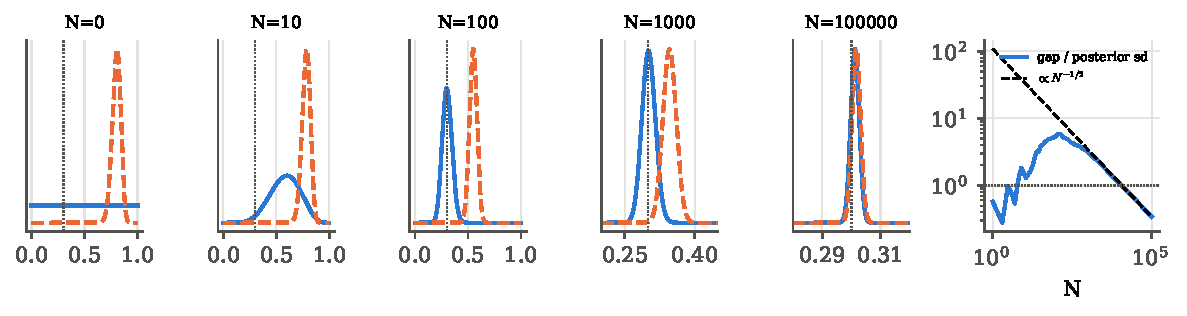
\includegraphics[width=\linewidth]{figures/ch05/bvm_converge.pdf}
\caption{Two analysts forget their priors. First five panels: posteriors from the flat
prior (solid) and from the confident prior $\mathrm{Beta}(80,20)$ (dashed) after
$N=0$ to $10^5$ tosses of a trigger with true efficiency $0.3$ (dotted). The horizontal
axis zooms in as the posteriors narrow. Last panel: the distance between the two
posterior means in units of the posterior width. It rises until $N$ is about the
prior's weight of 100, then falls as $N^{-1/2}$ (dashed line) and crosses one width
(dotted line) near $N=10^4$.}
\label{5b:fig:bvm-converge}
\end{figure}

\subsection{When the prior is never forgotten}

The derivation of \eqref{5b:eq:bvm-shift} used every condition in the key idea: enough
data, a prior nonzero at the truth, an identifiable parameter, a fixed number of
parameters, and a truth away from the edge. Each one can fail, and each failure shows up
in physics. We take them in turn.

\paragraph{Weak data.} The theorem is about large $N$. For $N$ comparable to the weight
$\kappa$ of an informative prior, or for a handful of events of any kind, the posterior
is a genuine compromise and the prior matters. After one trigger firing in ten muons the
three ``noninformative'' priors of \cref{5b:sec:priors} gave upper limits differing by a
third, and in the $N=10$ panel of \cref{5b:fig:bvm-converge} the two analysts are
$\FiveBBvmGapTen$ widths apart, with the gap still growing. With weak data the only
honest course is to report the prior and show how the answer moves when it changes: a
\newterm{prior sensitivity analysis} \srcref{Lambert}{\S5.7}.

\paragraph{A prior that is zero at the truth.} A health minister is ``morally certain''
that the prevalence of a disease is below 25\%, so the analysis uses a prior that is zero
above $0.25$ \srcref{Lambert}{\S5.7.1}. The true value is $0.3$. The posterior is prior
times likelihood, so it is zero above $0.25$ whatever the data say. As data accumulate
the likelihood climbs steadily towards $0.3$, and all the posterior can do is pile up
against the wall at $0.25$ (\cref{5b:fig:bvm-fail}, right). More data make the posterior
\emph{narrower at the wrong value}. The expansion \eqref{5b:eq:bvm-shift} failed because
$\ln p(\theta)=-\infty$ at the truth, so $g$ does not exist. A prior should be zero only
where a value is physically impossible.

\paragraph{A parameter the data cannot see.} A detector records the total count $n$ from
two channels with rates $\lambda_1$ and $\lambda_2$ but cannot tell them apart, so
$n\sim\text{Poisson}\bigl((\lambda_1+\lambda_2)T\bigr)$ in exposure $T$. What can the
count say about how the total is split between the channels? Reparametrise by the total
rate $\Lambda=\lambda_1+\lambda_2$ and the fraction $f=\lambda_1/\Lambda$ of the first
channel, and take independent priors $p(\Lambda)\,p(f)$. Then
\begin{align*}
  p(f\given n)
  &\eqby{1}\int p(\Lambda,f\given n)\,\dd\Lambda
   \eqby{2}\frac{\int\Prob(n\given\Lambda)\,p(\Lambda)\,p(f)\,\dd\Lambda}
               {\iint\Prob(n\given\Lambda')\,p(\Lambda')\,p(f')\,\dd\Lambda'\,\dd f'}
   \\
  &\eqby{3}p(f)\,\frac{\int\Prob(n\given\Lambda)\,p(\Lambda)\,\dd\Lambda}
               {\int\Prob(n\given\Lambda')\,p(\Lambda')\,\dd\Lambda'}
   =p(f).
\end{align*}
\begin{explain}
  \item Marginalise over the total rate (\cref{5b:sec:marginal}).
  \item Bayes' theorem. The likelihood depends on $\Lambda$ only, because the detector
        sees only the total.
  \item $p(f)$ comes out of the $\Lambda$ integral, and $\int p(f')\,\dd f'=1$.
\end{explain}
So the posterior of $f$ is its prior, exactly, for any number of counts. The data pin
down $\Lambda$ ever more precisely, but the prior alone decides the split. In the
simulation, $\FiveBBvmNtot$ counts fix $\Lambda$ to 1.4\%, yet two different priors on
$f$ give two completely different posteriors for $\lambda_1$ (\cref{5b:fig:bvm-fail},
left). Such a parameter is \newterm{not identifiable} \unpack{different values of it
predict exactly the same distribution of data}. Real cases are common: a
cosmological amplitude and a galaxy bias that enter only as a product, two
backgrounds with the same shape, a mass and a coupling that enter a rate only in
combination.

\paragraph{More parameters than data.} The theorem assumes the number of parameters
stays fixed while $N$ grows. Wasserman gives a simplified version of the Robins--Ritov
example, a missing-data problem with $B\gg N$ unknown probabilities $\theta_1,\dots,
\theta_B$ \mainref{pp.~186--188, Ex.~11.9}. With far fewer data than parameters, most
$\theta_j$ never appear in the likelihood, so their posterior equals their prior. The
posterior of their average $\psi=\frac1B\sum_j\theta_j$ therefore barely moves from its
prior. Yet a simple frequentist weighted average, the Horvitz--Thompson estimator, does
learn $\psi$: its error falls as $1/\sqrt N$ however large $B$ is. It succeeds because it
uses the known probability that each datum is observed. Those probabilities drop out of
the likelihood, so no method built on the likelihood can use them. Bayesian methods are
tied to the likelihood function, and in high-dimensional problems the likelihood may
not give accurate inferences.

\paragraph{A truth on the edge.} If the true value sits on the boundary of the allowed
range, such as a signal strength of exactly zero with the prior restricted to
nonnegative values, the posterior is a half-Gaussian piled against the edge, not a
Gaussian, and the credible and confidence intervals need not agree (\cref{ch:04}).

\begin{figure}[htbp]
\centering
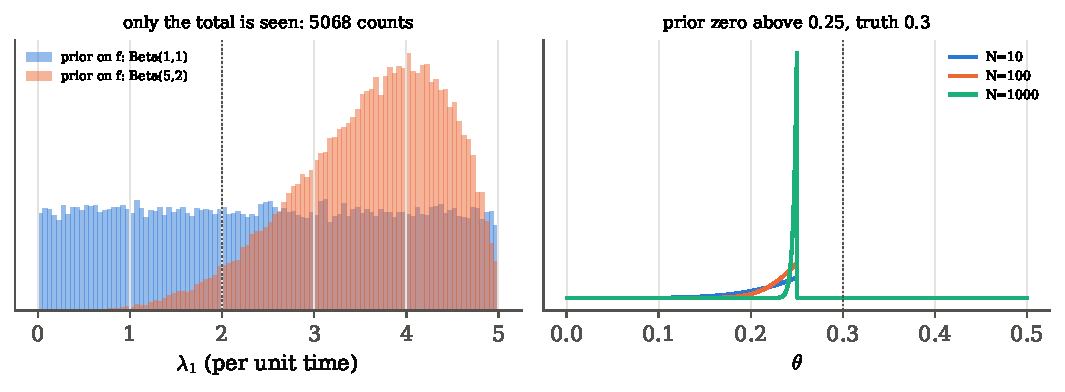
\includegraphics[width=\linewidth]{figures/ch05/bvm_fail.pdf}
\caption{Two ways the prior is never forgotten. Left: a detector that sees only the
total of two channels. With $\FiveBBvmNtot$ counts the total rate is known precisely,
but the posterior of the first channel's rate $\lambda_1$ is set by the prior on its
fraction: a flat prior gives the broad blue histogram, a $\mathrm{Beta}(5,2)$ prior the
orange one. The dotted line is the true $\lambda_1=2$. Right: a prior that is zero above
$0.25$ when the truth is $0.3$ (dotted). With 10, 100 and 1000 data the posterior only
piles up more sharply against the wall.}
\label{5b:fig:bvm-fail}
\end{figure}

\subsection{Forgetting the prior is not forgetting the start of a chain}

When a posterior cannot be computed on a grid, we explore it with a Markov chain: a
random walk in parameter space, biased so that it spends time in each region in
proportion to the posterior there (\cref{ch:09}). A chain started far from the bulk of
the posterior wanders for a while before it settles. That early part, the
\newterm{burn-in}, is thrown away, and after it the chain has forgotten where it
started. It is tempting to say the chain has also ``washed out'' the prior. It has not,
because the two forgettings work by different mechanisms.
\begin{itemize}
  \item \emph{A chain forgets its starting point} because every step is drawn from a
        rule that leaves one target distribution unchanged, and repeated steps pull any
        starting distribution towards that target (\cref{ch:09} proves the contraction).
        Running the chain longer is the cure for a bad start.
  \item \emph{A posterior forgets its prior} only through the likelihood,
        \eqref{5b:eq:bvm-ratio}: more \emph{data}. The target of the chain is
        prior$\times$likelihood, prior included, so a chain run forever reproduces the
        prior's influence perfectly.
\end{itemize}

\paragraph{Example: four chains.} Take 6 firings in 20 muons and the two priors of the
trigger example. We run a Metropolis chain \unpack{a random walk whose proposed steps are
accepted or rejected by comparing posterior values} from $\theta=0.02$ and from
$\theta=0.98$ for each prior, $2\times10^4$ steps each, and discard the first 5000.

\pyfile[firstline=94,lastline=108,firstnumber=94]{code/ch05/15_bvm.py}{A Metropolis
chain on the trigger posterior: only a ratio of posteriors enters}

Lines~94--97 are the log-posterior, $\ln[\theta^{z+a-1}(1-\theta)^{N-z+b-1}]$ up to a
constant, and $-\infty$ outside $(0,1)$. Line~103 proposes a Gaussian step. Line~105
accepts it with probability $\min(1,p_{\text{new}}/p_{\text{old}})$. This is computed
from the difference of log-posteriors, so the unknown evidence cancels and never
appears.

The results separate the two forgettings (\cref{5b:fig:chain-prior}). With the flat
prior the two chains give means $\FiveBChainFlatA$ and $\FiveBChainFlatB$ from their two
starts, against the exact posterior mean $\FiveBChainExactFlat$. With the confident prior
they give $\FiveBChainStrA$ and $\FiveBChainStrB$, against the exact
$\FiveBChainExactStr$. Within a few dozen steps each chain has forgotten whether it
started at $0.02$ or $0.98$. But no number of steps brings the two priors together:
they sample two different posteriors, both correctly. Only more muons would.

\begin{figure}[htbp]
\centering
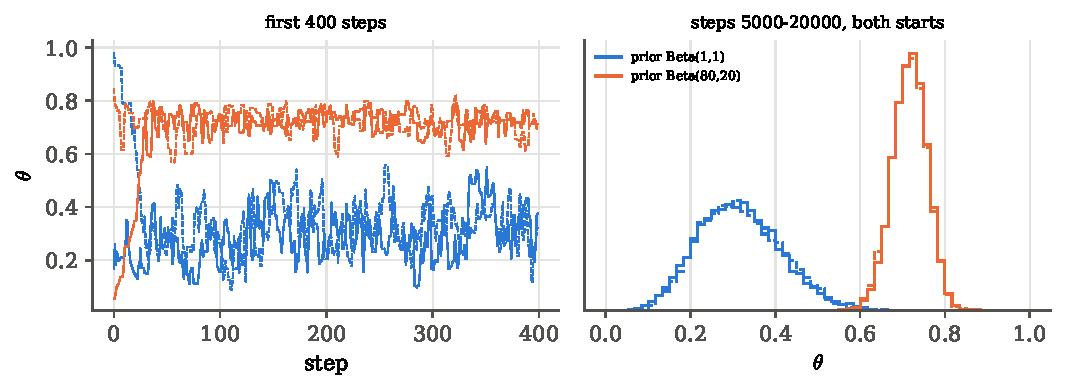
\includegraphics[width=\linewidth]{figures/ch05/chain_vs_prior.pdf}
\caption{Two kinds of forgetting. Left: the first 400 steps of four Metropolis chains on
the trigger posterior after 6 firings in 20 muons, started at $0.02$ (solid) and $0.98$
(dashed), with the flat prior (blue) and the confident prior (orange). Each pair forgets
its start within a few dozen steps. Right: histograms of steps 5000 to 20000. Chains with
the same prior agree whatever the start. Chains with different priors disagree however
long they run.}
\label{5b:fig:chain-prior}
\end{figure}

\begin{pitfall}[Burn-in does not remove a prior]
Discarding burn-in removes the memory of the chain's starting point. It does nothing to
the prior, which is part of the distribution the chain is built to sample. If two
analyses with different priors disagree, running the chains longer will only make the
disagreement more precise. The cure is more informative data, or a prior sensitivity
analysis that reports how the result depends on the prior.
\end{pitfall}
\section{Sampling the posterior: a histogram instead of an integral}
\label{5b:sec:sampling}

A mass on a spring oscillates as $x(t)=A\cos\omega t$. Where are we most likely to find
it if we look at a random moment? ``A random moment'' already contains an assumption:
the moment of looking is uniform in time, so the phase $\omega t$ is uniform over a
cycle. With that assumption there are two ways to answer. One is a calculation: change
variables from the uniform phase to the position and obtain the arcsine density
$1/(\pi\sqrt{A^2-x^2})$ (\cref{ch:01}). The other needs no calculus at all. Pick a large
set of random times, compute $x$ at each, and histogram the values. The histogram piles
up at the turning points, where the mass moves slowly, and it traces out the arcsine
curve (\cref{5b:fig:sampling}, bottom right). This idea can be used to find the
probability distribution of position: we plot the histogram for $x$ for a large set of
random values of $t$.

The same idea works for a posterior. Suppose that instead of a formula for
$p(\theta\given\data)$ we had a machine that produces random values
$\theta_1,\dots,\theta_B$ distributed according to it. Then a histogram of
$\theta_1,\dots,\theta_B$ approximates the posterior density $p(\theta\given\data)$
\mainref{p.~180}. Every integral we have needed so far becomes a count or an average
over the draws: a mean, a marginal, the probability of an interval. This is the bridge
from Bayesian inference to Monte Carlo, and it is how almost all modern posteriors are
handled.

The question, in words: if we can draw from the posterior, what can we compute from the
draws, and how accurately?

\begin{workdef}[posterior sample]
A \newterm{posterior sample} is a set of values $\theta_1,\dots,\theta_B$, each drawn from
$p(\theta\given\data)$ \unpack{so that the fraction of draws in any interval approaches
the posterior probability of that interval as $B$ grows}. \emph{Operationally:} the
posterior probability of a set $S$ is estimated by the fraction of draws in $S$, the
posterior mean of any function $g(\theta)$ by $\frac1B\sum_ig(\theta_i)$, and a quantile
by the corresponding order statistic of the sorted draws.
\end{workdef}

\subsection{Why a histogram of draws is the density}

Take a bin of width $\Delta$ around $\theta_j$. Each draw lands in it independently with
probability $P_j=\int_{\text{bin}}p(\theta\given\data)\,\dd\theta\approx p(\theta_j\given
\data)\,\Delta$, so the count $n_j$ in the bin is binomial, $n_j\sim\mathrm{Bin}(B,P_j)$
(\cref{ch:02}). The histogram height, count divided by $B\Delta$, then has
\begin{align*}
  \E\Bigl[\frac{n_j}{B\Delta}\Bigr]
  &\eqby{1}\frac{BP_j}{B\Delta}\relby{2}{\approx} p(\theta_j\given\data),
  \\
  \frac{\text{sd}(n_j)}{\E[n_j]}
  &\eqby{3}\frac{\sqrt{BP_j(1-P_j)}}{BP_j}
   \relby{4}{\approx}\frac{1}{\sqrt{BP_j}} .
\end{align*}
\begin{explain}
  \item The mean of a binomial count is $BP_j$.
  \item $P_j\approx p(\theta_j\given\data)\Delta$ for a narrow bin.
  \item The standard deviation of a binomial count is $\sqrt{BP_j(1-P_j)}$.
  \item A single bin holds a small fraction of the probability, $P_j\ll1$.
\end{explain}
So the histogram is centred on the density. Its relative error in a bin is one over the
square root of the expected count there. For example, with $B=\FiveBSaB$ draws and a bin
holding 1\% of the probability, the expected count is 2000 and the height is good to
about $1/\sqrt{2000}\approx2\%$. The
same counting argument says that averages over draws converge: the average of $g(\theta_i)$
has mean $\E[g(\theta)\given\data]$ and standard deviation $\text{sd}(g)/\sqrt B$ for
independent draws \mainref{p.~181}.

\begin{pitfall}[Monte Carlo error is not the error bar]
Two different widths appear. The \emph{posterior width} $\text{sd}(\theta\given\data)$ is
the physical uncertainty on the parameter. It is set by the data and does not shrink when
we draw more samples. The \emph{Monte Carlo error} $\text{sd}(\theta\given\data)/\sqrt B$ is
how well the draws reproduce the exact posterior mean. It shrinks with $B$ and says nothing
about the physics. Quote the first as the error bar. Make sure the second is much smaller.
\end{pitfall}

\subsection{What the draws give for free}

\Cref{5b:fig:draws-flow} collects the operations. Each of them replaces an integral by a
one-line manipulation of an array of draws.

\begin{figure}[htbp]
\centering
\begin{tikzpicture}[x=1cm,y=1cm,
  box/.style={draw,rounded corners,fill=white,align=center,font=\footnotesize,
               inner sep=3pt,text width=1.95cm},
  arr/.style={->,thick,black!65}]
  \node[box,fill=formblue!10,text width=4.6cm] (d) at (0,0) {draws\\ $\params_1,\dots,\params_B\sim p(\params\given\data)$};
  \node[box] (h) at (-4.8,-2.3) {histogram\\ $\to$ density};
  \node[box] (m) at (-2.4,-2.3) {average, sort\\ $\to$ mean, interval};
  \node[box] (g) at (0,-2.3) {$\tau_i=g(\params_i)$\\ $\to$ any function};
  \node[box] (k) at (2.4,-2.3) {keep one coordinate\\ $\to$ marginal};
  \node[box] (p) at (4.8,-2.3) {$\tilde x_i\sim p(\tilde x\given\params_i)$\\ $\to$ new data};
  \foreach \t in {h,m,g,k,p}{\draw[arr] (d.south) -- (\t.north);}
\end{tikzpicture}
\caption{One array of posterior draws, five products. Histogramming it approximates the
density. Averaging and sorting give the mean and the interval ends. Applying a function
to each draw gives draws of that function. Ignoring all but one coordinate gives draws of
that parameter's marginal. Simulating a new data set from each draw gives the
distribution of future data.}
\label{5b:fig:draws-flow}
\end{figure}

\paragraph{Means and intervals.} The posterior mean is estimated by $\frac1B\sum_i
\theta_i$. The ends of the 95\% equal-tailed interval are the 2.5\% and 97.5\% sample
quantiles, and the HDI is the shortest window that contains 95\% of the sorted draws
(\cref{5b:sec:summaries}) \mainref{p.~181}.

\paragraph{Functions of the parameter.} If $\tau=g(\theta)$, then $\tau_i=g(\theta_i)$ is
a sample from the posterior of $\tau$. No change of variables is needed
\mainref{pp.~180--181}. To see how much work this saves, take a coin's heads probability
$p$ after $s=10$ heads in $n=14$ tosses, with a flat prior. Write $x^n=(x_1,\dots,x_n)$
for the tosses. The posterior is $p\given x^n\sim\mathrm{Beta}(s+1,n-s+1)$
(\cref{5b:sec:conjugate}). What is the posterior density of the log-odds
$\psi=\ln[p/(1-p)]$? The exact route goes through the cumulative distribution $H$ of
$\psi$, and then its derivative $h$:
\begin{align*}
  H(\psi\given x^n)
  &\eqby{1}\Prob\Bigl(\ln\frac{P}{1-P}\le\psi\Bigm| x^n\Bigr)
   \eqby{2}\Prob\Bigl(P\le\frac{e^\psi}{1+e^\psi}\Bigm| x^n\Bigr)
   \eqby{3}\int_0^{e^\psi/(1+e^\psi)}f(p\given x^n)\,\dd p,\\
  h(\psi\given x^n)
  &\eqby{4}f\Bigl(\frac{e^\psi}{1+e^\psi}\Bigm| x^n\Bigr)\,\frac{e^\psi}{(1+e^\psi)^2}
   \eqby{5}\frac{\Gamma(n+2)}{\Gamma(s+1)\Gamma(n-s+1)}
     \Bigl(\frac{e^\psi}{1+e^\psi}\Bigr)^{s+1}\Bigl(\frac{1}{1+e^\psi}\Bigr)^{n-s+1}.
\end{align*}
\begin{explain}
  \item Definition of the cumulative distribution of $\Psi=\ln[P/(1-P)]$, with $P$ the
        random heads probability.
  \item The log-odds is increasing in $P$, so the inequality can be inverted.
  \item The probability of an interval is the integral of the posterior density over it.
  \item Differentiate with respect to $\psi$: fundamental theorem of calculus and chain
        rule, with $\dd p/\dd\psi$ from \eqref{5b:eq:logit-density}.
  \item Insert the Beta density $f(p\given x^n)=\frac{\Gamma(n+2)}{\Gamma(s+1)\Gamma(n-s+1)}
        p^s(1-p)^{n-s}$ at $p=e^\psi/(1+e^\psi)$, and note that $\frac{e^\psi}{(1+e^\psi)^2}
        =p(1-p)$ raises each power by one.
\end{explain}
This is Wasserman's Example 11.3 \mainref{p.~180}. The sampling route takes two lines:
draw $P_i\sim\mathrm{Beta}(11,5)$, set $\psi_i=\ln[P_i/(1-P_i)]$, and histogram
\mainref{p.~181, Ex.~11.4}. The two agree (\cref{5b:fig:sampling}, top left). For a
function of several parameters, or one with no inverse in closed form, the sampling
route is the only practical one.

\paragraph{Marginals and combinations.} Take several parameters $\params=(\theta_1,\dots,
\theta_p)$ and $B$ draws $\params^{(1)},\dots,\params^{(B)}$. Their first coordinates
$\theta_1^{(1)},\dots,\theta_1^{(B)}$ are a sample from the marginal posterior of
$\theta_1$. Keeping one coordinate and ignoring the rest replaces the $(p-1)$-dimensional
integral of \cref{5b:sec:marginal} \mainref{p.~183, (11.9)}.

A combination of parameters is just as easy. After a detector upgrade we want to know:
did the efficiency improve? Before the upgrade $x_1=18$ of $n_1=40$ test pulses were
detected, and after it $x_2=28$ of $n_2=40$. Call the two efficiencies $p_1$ and $p_2$.
With a flat prior on the square $(p_1,p_2)\in[0,1]^2$,
\begin{equation*}
  p(p_1,p_2\given x_1,x_2)\propto p_1^{x_1}(1-p_1)^{n_1-x_1}\;p_2^{x_2}(1-p_2)^{n_2-x_2},
\end{equation*}
which factorises into $\mathrm{Beta}(x_1+1,n_1-x_1+1)$ for $p_1$ times
$\mathrm{Beta}(x_2+1,n_2-x_2+1)$ for $p_2$: under the posterior the two efficiencies are
independent \mainref{pp.~183--184, Ex.~11.7}. The improvement is $\tau=p_2-p_1$. Draw
$B$ values of each efficiency and subtract, $\tau_i=p_{2,i}-p_{1,i}$. The fraction of
positive differences estimates $\Prob(p_2>p_1\given\data)=\FiveBSaPpos$, and the 95\%
interval for the improvement is $(\FiveBSaTauLo,\FiveBSaTauHi)$ (\cref{5b:fig:sampling},
bottom left). If the parameters were correlated, the same subtraction of draws would use
the correlation automatically, because each draw is a pair taken together. The separate
marginals would have thrown that correlation away.

\paragraph{Predicting new data.} The \newterm{posterior predictive distribution} of a
future data set $\tilde x$ averages the forward model over our uncertainty about $\theta$:
\begin{align*}
  p(\tilde x\given\data)
  &\eqby{1}\int p(\tilde x,\theta\given\data)\,\dd\theta
   \eqby{2}\int p(\tilde x\given\theta,\data)\,p(\theta\given\data)\,\dd\theta
   \eqby{3}\int p(\tilde x\given\theta)\,p(\theta\given\data)\,\dd\theta .
\end{align*}
\begin{explain}
  \item Sum rule: marginalise the joint distribution of new data and parameter.
  \item Product rule.
  \item Given $\theta$, the new data are independent of the old data: the old data
        influence the prediction only through what they tell us about $\theta$.
\end{explain}
The sampling recipe mirrors the formula: for each draw $\theta_i$, simulate one new data
set $\tilde x_i$ from $p(\tilde x\given\theta_i)$. The collection $\tilde x_1,\dots,
\tilde x_B$ is a sample from the predictive distribution \srcref{Lambert}{\S7.8}.

\paragraph{Example: two more heads.} After 10 heads in 14 tosses, what is the probability
that the next two tosses are both heads? The exact answer, found in
\cref{5b:sec:conjugate}, is $B(13,5)/B(11,5)=\FiveBSaTwoHeadsExact$, not the plug-in
$(10/14)^2=0.51$ \srcref{Padilla}{\S2.3}. By sampling: for each draw $p_i$, toss two
simulated coins with heads probability $p_i$ and record whether both came up heads. The
fraction is $\FiveBSaTwoHeads$, within the Monte Carlo error $\sqrt{0.485\times0.515/B}
\approx0.001$ of the exact value.

\paragraph{Example: failures in the next batch.} One detector module in a batch of ten
fails its burn-in test. How many failures should we expect in the next batch of ten?
\begin{itemize}[itemsep=1pt,leftmargin=1.2em]
  \item \emph{Plug-in.} Take the failure rate to be exactly $0.1$ and use
        $\mathrm{Bin}(10,0.1)$. Its central 80\% range is $0$ to $\FiveBSaPlugHi$
        failures.
  \item \emph{Posterior predictive.} With a flat prior the posterior of the rate is
        $\mathrm{Beta}(1+1,1+9)=\mathrm{Beta}(2,10)$. Draw a rate, then a batch of ten
        with that rate, and repeat. The central 80\% range is $\FiveBSaPredLo$ to
        $\FiveBSaPredHi$ (\cref{5b:fig:sampling}, top right) \srcref{Lambert}{\S7.8}.
\end{itemize}
The predictive range is wider because it includes two sources of spread: our
uncertainty about the rate, and the binomial scatter of a batch. It also gives zero
failures probability $\FiveBSaPredZero$, against the plug-in $\FiveBSaPlugZero$, because
the rate could well be larger than $0.1$. Plugging in a best value always makes
predictions look more certain than they are.

\subsection{The same code for every posterior}

\pyfile[firstline=33,lastline=75,firstnumber=33]{code/ch05/16_sampling.py}{Posterior
draws put to work: a function of the parameter, two predictive calculations and a
difference of two efficiencies}

Lines~35--36 draw $B$ values of the heads probability from $\mathrm{Beta}(11,5)$ and turn
each into a log-odds, and line~39 is the exact density from the chain above, used only as
a check. Line~47 is the two-heads prediction: two uniform numbers per draw, each below
$p_i$ with probability $p_i$. Lines~49--50 draw a failure rate and then a whole new batch
for each draw, and lines~54--55 read the 80\% predictive range off the cumulative
histogram. Lines~66--68 draw the two efficiencies independently and subtract them, and
lines~74--75 turn the differences into a probability and an interval. The last panel of
the figure is the oscillator: uniform phases, $x=A\cos\omega t$, histogram. It is the
same three lines as the log-odds, with a random phase in the place of a random heads
probability.

\begin{figure}[htbp]
\centering
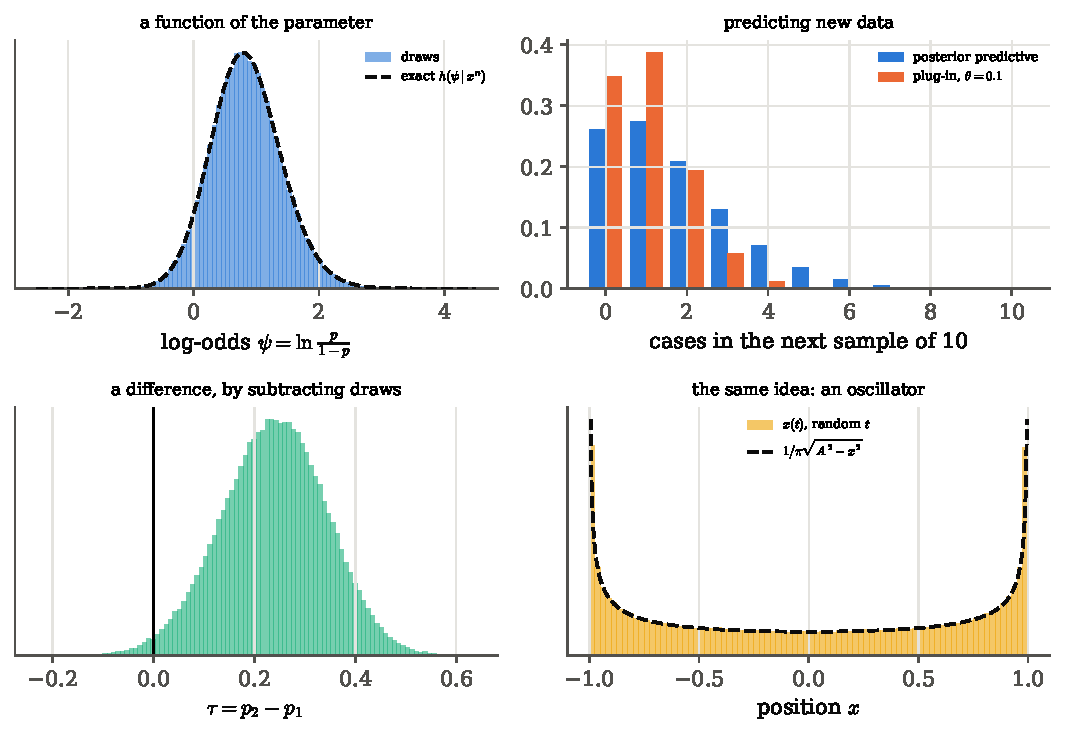
\includegraphics[width=0.95\linewidth]{figures/ch05/sampling.pdf}
\caption{Posterior draws at work. Top left: draws of the heads probability after 10 heads
in 14, turned into log-odds and histogrammed, against the exact density (dashed). Top
right: the predicted number of failures in the next batch of ten modules after one
failure in ten, from posterior draws (blue) and from plugging in the rate $0.1$ (orange).
Bottom left: the improvement in efficiency, from differences of draws. Bottom right: the
same idea for an oscillator. Positions at uniformly random times follow the arcsine
density (dashed).}
\label{5b:fig:sampling}
\end{figure}

Here every draw came from a standard generator, because every posterior was a Beta
density. That is the luxury of conjugacy (\cref{5b:sec:conjugate}). For a realistic
posterior in six or twenty dimensions we have neither a grid nor a generator. We can
only evaluate $\Like(\params)\,p(\params)$ at any point we choose. Monte Carlo methods
turn uniform random numbers into draws from simple distributions (\cref{ch:06}), and Markov
chain Monte Carlo builds a random walk whose visited points are draws from a posterior
known only up to its normalising constant (\cref{ch:09}). Everything downstream of the
draws, the histograms, averages, quantiles, functions, marginals and predictions of this
section, stays exactly the same.

\begin{recap}
\begin{itemize}
  \item For a continuous parameter, the observed data are the event, the parameter values
        are the hypotheses, and $p(\lambda\given\data)=\Like(\lambda)p(\lambda)/p(\data)$
        is a density. On a grid, sum log-likelihoods and subtract the maximum before
        exponentiating.
  \item Conjugate pairs (Beta--Binomial, Gamma--Poisson, Gaussian--Gaussian) give exact
        posteriors. In the Gaussian case precisions add and means are
        precision-weighted.
  \item Summaries: the posterior mean, median and mode minimise squared, absolute and
        all-or-nothing loss. Equal-tailed intervals are invariant under reparametrisation.
        HDIs are the shortest.
  \item Near a single peak the posterior is Gaussian with covariance minus the inverse
        Hessian of $\ln p$. Marginal errors come from the diagonal of the inverse.
  \item Nuisance parameters are integrated out. Profiling maximises over them instead, and
        the two differ by a volume factor.
  \item No prior is flat in every parametrisation. Jeffreys' prior $\sqrt{I(\theta)}$ is
        coordinate independent: $1/\sigma$ for a scale, $\mathrm{Beta}(\frac12,\frac12)$
        for a Bernoulli probability.
  \item With many data a smooth prior's influence dies as $N^{-1/2}$ posterior widths
        (Bernstein--von Mises). It is never forgotten if it is zero at the truth, if the
        parameter is not identifiable, or if parameters outnumber data. A Markov chain
        forgets its start, not its prior.
  \item A histogram of posterior draws is the posterior. Functions, marginals and
        predictions of new data are one line each on the draws.
\end{itemize}
\end{recap}

\providecommand{\FiveCFacZone}{}\renewcommand{\FiveCFacZone}{4.993\times10^{-4}}
\providecommand{\FiveCFacZtwo}{}\renewcommand{\FiveCFacZtwo}{0.002339}
\providecommand{\FiveCFacZgridOne}{}\renewcommand{\FiveCFacZgridOne}{4.993\times10^{-4}}
\providecommand{\FiveCFacZgridTwo}{}\renewcommand{\FiveCFacZgridTwo}{0.002339}
\providecommand{\FiveCFacBF}{}\renewcommand{\FiveCFacBF}{0.2135}
\providecommand{\FiveCFacInvBF}{}\renewcommand{\FiveCFacInvBF}{4.683}
\providecommand{\FiveCFacPostOne}{}\renewcommand{\FiveCFacPostOne}{17.6}
\providecommand{\FiveCFacPostTwo}{}\renewcommand{\FiveCFacPostTwo}{82.4}
\providecommand{\FiveCFairFifteen}{}\renewcommand{\FiveCFairFifteen}{0.3229}
\providecommand{\FiveCFairEleven}{}\renewcommand{\FiveCFairEleven}{3.337}
\providecommand{\FiveCFairTen}{}\renewcommand{\FiveCFairTen}{3.664}
\providecommand{\FiveCFacMeanOne}{}\renewcommand{\FiveCFacMeanOne}{0.4524}
\providecommand{\FiveCFacMeanTwo}{}\renewcommand{\FiveCFacMeanTwo}{0.6905}
\providecommand{\FiveCFacMeanAvg}{}\renewcommand{\FiveCFacMeanAvg}{0.6486}
\providecommand{\FiveCFairZmin}{}\renewcommand{\FiveCFairZmin}{7}
\providecommand{\FiveCFairZmax}{}\renewcommand{\FiveCFairZmax}{13}
\providecommand{\FiveCBumpChiLine}{}\renewcommand{\FiveCBumpChiLine}{49.07}
\providecommand{\FiveCBumpChiBump}{}\renewcommand{\FiveCBumpChiBump}{34.54}
\providecommand{\FiveCBumpDChi}{}\renewcommand{\FiveCBumpDChi}{14.53}
\providecommand{\FiveCBumplnLR}{}\renewcommand{\FiveCBumplnLR}{7.265}
\providecommand{\FiveCBumplnB}{}\renewcommand{\FiveCBumplnB}{2.096}
\providecommand{\FiveCBumplnOccam}{}\renewcommand{\FiveCBumplnOccam}{-5.169}
\providecommand{\FiveCBumpB}{}\renewcommand{\FiveCBumpB}{8.133}
\providecommand{\FiveCBumpAhat}{}\renewcommand{\FiveCBumpAhat}{2.307}
\providecommand{\FiveCBumpMuhat}{}\renewcommand{\FiveCBumpMuhat}{6.373}
\providecommand{\FiveCBumplnZline}{}\renewcommand{\FiveCBumplnZline}{-68.61}
\providecommand{\FiveCBumplnZbump}{}\renewcommand{\FiveCBumplnZbump}{-66.51}
\providecommand{\FiveCBumpGridErr}{}\renewcommand{\FiveCBumpGridErr}{1.236\times10^{-8}}
\providecommand{\FiveCFlatChiLine}{}\renewcommand{\FiveCFlatChiLine}{48.37}
\providecommand{\FiveCFlatChiBump}{}\renewcommand{\FiveCFlatChiBump}{43.98}
\providecommand{\FiveCFlatDChi}{}\renewcommand{\FiveCFlatDChi}{4.387}
\providecommand{\FiveCFlatlnLR}{}\renewcommand{\FiveCFlatlnLR}{2.194}
\providecommand{\FiveCFlatlnB}{}\renewcommand{\FiveCFlatlnB}{-1.675}
\providecommand{\FiveCFlatlnOccam}{}\renewcommand{\FiveCFlatlnOccam}{-3.868}
\providecommand{\FiveCFlatB}{}\renewcommand{\FiveCFlatB}{0.1873}
\providecommand{\FiveCFlatAhat}{}\renewcommand{\FiveCFlatAhat}{1.584}
\providecommand{\FiveCFlatMuhat}{}\renewcommand{\FiveCFlatMuhat}{0.2214}
\providecommand{\FiveCFlatlnZline}{}\renewcommand{\FiveCFlatlnZline}{-68.26}
\providecommand{\FiveCFlatlnZbump}{}\renewcommand{\FiveCFlatlnZbump}{-69.93}
\providecommand{\FiveCFlatGridErr}{}\renewcommand{\FiveCFlatGridErr}{7.607\times10^{-6}}
\providecommand{\FiveCLapLnZbump}{}\renewcommand{\FiveCLapLnZbump}{-66.57}
\providecommand{\FiveCLapLnB}{}\renewcommand{\FiveCLapLnB}{2.04}
\providecommand{\FiveCLapLnOccOne}{}\renewcommand{\FiveCLapLnOccOne}{-12.54}
\providecommand{\FiveCLapLnOccZero}{}\renewcommand{\FiveCLapLnOccZero}{-7.318}
\providecommand{\FiveCLapOccRatio}{}\renewcommand{\FiveCLapOccRatio}{0.005381}
\providecommand{\FiveCSigA}{}\renewcommand{\FiveCSigA}{0.6053}
\providecommand{\FiveCSigMu}{}\renewcommand{\FiveCSigMu}{0.1415}
\providecommand{\FiveCSigAMuVol}{}\renewcommand{\FiveCSigAMuVol}{0.5381}
\providecommand{\FiveCPriorAMuVol}{}\renewcommand{\FiveCPriorAMuVol}{100}
\providecommand{\FiveCFixLnB}{}\renewcommand{\FiveCFixLnB}{4.668}
\providecommand{\FiveCFixB}{}\renewcommand{\FiveCFixB}{106.5}
\providecommand{\FiveCFreeOverFix}{}\renewcommand{\FiveCFreeOverFix}{13.09}
\providecommand{\FiveCFixAhat}{}\renewcommand{\FiveCFixAhat}{2.18}
\providecommand{\FiveCFixSigA}{}\renewcommand{\FiveCFixSigA}{0.6018}
\providecommand{\FiveCFixZscore}{}\renewcommand{\FiveCFixZscore}{3.622}
\providecommand{\FiveCBumpLnBHundred}{}\renewcommand{\FiveCBumpLnBHundred}{-0.2067}
\providecommand{\FiveCFlatLnBHundred}{}\renewcommand{\FiveCFlatLnBHundred}{-3.977}
\providecommand{\FiveCFlatLnBOne}{}\renewcommand{\FiveCFlatLnBOne}{-0.03148}
\providecommand{\FiveCAmax}{}\renewcommand{\FiveCAmax}{10}
\providecommand{\FiveCNdata}{}\renewcommand{\FiveCNdata}{40}
\providecommand{\FiveCWidth}{}\renewcommand{\FiveCWidth}{0.5}
\providecommand{\FiveCTrueA}{}\renewcommand{\FiveCTrueA}{2.5}
\providecommand{\FiveCTrueMu}{}\renewcommand{\FiveCTrueMu}{6.2}
\providecommand{\FiveCHalUnifBF}{}\renewcommand{\FiveCHalUnifBF}{0.1253}
\providecommand{\FiveCHalHaldBF}{}\renewcommand{\FiveCHalHaldBF}{5.728}
\providecommand{\FiveCInfUnifBF}{}\renewcommand{\FiveCInfUnifBF}{0.05571}
\providecommand{\FiveCInfHaldBF}{}\renewcommand{\FiveCInfHaldBF}{0.05748}
\providecommand{\FiveCHdiUnifLo}{}\renewcommand{\FiveCHdiUnifLo}{0.5543}
\providecommand{\FiveCHdiUnifHi}{}\renewcommand{\FiveCHdiUnifHi}{0.7382}
\providecommand{\FiveCHdiHaldLo}{}\renewcommand{\FiveCHdiHaldLo}{0.5564}
\providecommand{\FiveCHdiHaldHi}{}\renewcommand{\FiveCHdiHaldHi}{0.7418}
\providecommand{\FiveCLamS}{}\renewcommand{\FiveCLamS}{75}
\providecommand{\FiveCLamT}{}\renewcommand{\FiveCLamT}{150}
\providecommand{\FiveCLamLnZa}{}\renewcommand{\FiveCLamLnZa}{-32.78}
\providecommand{\FiveCLamLnZb}{}\renewcommand{\FiveCLamLnZb}{-28.86}
\providecommand{\FiveCLamLnZc}{}\renewcommand{\FiveCLamLnZc}{-27.66}
\providecommand{\FiveCLamZratio}{}\renewcommand{\FiveCLamZratio}{50.36}
\providecommand{\FiveCLamMeanA}{}\renewcommand{\FiveCLamMeanA}{0.5}
\providecommand{\FiveCLamMeanB}{}\renewcommand{\FiveCLamMeanB}{0.5}
\providecommand{\FiveCLamSdA}{}\renewcommand{\FiveCLamSdA}{0.04069}
\providecommand{\FiveCLamSdB}{}\renewcommand{\FiveCLamSdB}{0.04043}
\providecommand{\FiveCLinPzeroN}{}\renewcommand{\FiveCLinPzeroN}{0.3512}
\providecommand{\FiveCLinPzeroNk}{}\renewcommand{\FiveCLinPzeroNk}{0.8228}
\providecommand{\FiveCLinPzeroNm}{}\renewcommand{\FiveCLinPzeroNm}{0.9932}
\providecommand{\FiveCLinPzeroNkk}{}\renewcommand{\FiveCLinPzeroNkk}{0.9731}
\providecommand{\FiveCLinNhalf}{}\renewcommand{\FiveCLinNhalf}{41.25}
\providecommand{\FiveCLinBound}{}\renewcommand{\FiveCLinBound}{0.1278}
\providecommand{\FiveCLinBoundLR}{}\renewcommand{\FiveCLinBoundLR}{6.826}
\providecommand{\FiveCSelaB}{}\renewcommand{\FiveCSelaB}{2.456}
\providecommand{\FiveCSelalnB}{}\renewcommand{\FiveCSelalnB}{0.8985}
\providecommand{\FiveCSelaZ}{}\renewcommand{\FiveCSelaZ}{1.96}
\providecommand{\FiveCSelbB}{}\renewcommand{\FiveCSelbB}{7.988}
\providecommand{\FiveCSelblnB}{}\renewcommand{\FiveCSelblnB}{2.078}
\providecommand{\FiveCSelbZ}{}\renewcommand{\FiveCSelbZ}{2.576}
\providecommand{\FiveCSelcB}{}\renewcommand{\FiveCSelcB}{21.11}
\providecommand{\FiveCSelclnB}{}\renewcommand{\FiveCSelclnB}{3.05}
\providecommand{\FiveCSelcZ}{}\renewcommand{\FiveCSelcZ}{2.968}
\providecommand{\FiveCSeldB}{}\renewcommand{\FiveCSeldB}{53.26}
\providecommand{\FiveCSeldlnB}{}\renewcommand{\FiveCSeldlnB}{3.975}
\providecommand{\FiveCSeldZ}{}\renewcommand{\FiveCSeldZ}{3.291}
\providecommand{\FiveCSeleB}{}\renewcommand{\FiveCSeleB}{151.2}
\providecommand{\FiveCSelelnB}{}\renewcommand{\FiveCSelelnB}{5.018}
\providecommand{\FiveCSeleZ}{}\renewcommand{\FiveCSeleZ}{3.615}
\providecommand{\FiveCSelfB}{}\renewcommand{\FiveCSelfB}{44889}
\providecommand{\FiveCSelflnB}{}\renewcommand{\FiveCSelflnB}{10.71}
\providecommand{\FiveCSelfZ}{}\renewcommand{\FiveCSelfZ}{5.001}
\providecommand{\FiveCHmOnelnZZero}{}\renewcommand{\FiveCHmOnelnZZero}{-68.61}
\providecommand{\FiveCHmOnePZero}{}\renewcommand{\FiveCHmOnePZero}{0.07901}
\providecommand{\FiveCHmOneChiZero}{}\renewcommand{\FiveCHmOneChiZero}{49.07}
\providecommand{\FiveCHmOneBICZero}{}\renewcommand{\FiveCHmOneBICZero}{56.44}
\providecommand{\FiveCHmOneAICZero}{}\renewcommand{\FiveCHmOneAICZero}{53.07}
\providecommand{\FiveCHmOnelnZOne}{}\renewcommand{\FiveCHmOnelnZOne}{-66.51}
\providecommand{\FiveCHmOnePOne}{}\renewcommand{\FiveCHmOnePOne}{0.6425}
\providecommand{\FiveCHmOneChiOne}{}\renewcommand{\FiveCHmOneChiOne}{34.54}
\providecommand{\FiveCHmOneBICOne}{}\renewcommand{\FiveCHmOneBICOne}{49.29}
\providecommand{\FiveCHmOneAICOne}{}\renewcommand{\FiveCHmOneAICOne}{42.54}
\providecommand{\FiveCHmOnelnZTwo}{}\renewcommand{\FiveCHmOnelnZTwo}{-67.35}
\providecommand{\FiveCHmOnePTwo}{}\renewcommand{\FiveCHmOnePTwo}{0.2784}
\providecommand{\FiveCHmOneChiTwo}{}\renewcommand{\FiveCHmOneChiTwo}{30.1}
\providecommand{\FiveCHmOneBICTwo}{}\renewcommand{\FiveCHmOneBICTwo}{52.24}
\providecommand{\FiveCHmOneAICTwo}{}\renewcommand{\FiveCHmOneAICTwo}{42.1}
\providecommand{\FiveCHmOnelnBtwoone}{}\renewcommand{\FiveCHmOnelnBtwoone}{-0.8362}
\providecommand{\FiveCHmOnelnBonezero}{}\renewcommand{\FiveCHmOnelnBonezero}{2.096}
\providecommand{\FiveCHmOneBICtwoone}{}\renewcommand{\FiveCHmOneBICtwoone}{-1.473}
\providecommand{\FiveCHmOneBIConezero}{}\renewcommand{\FiveCHmOneBIConezero}{3.576}
\providecommand{\FiveCHmTwolnZZero}{}\renewcommand{\FiveCHmTwolnZZero}{-75.73}
\providecommand{\FiveCHmTwoPZero}{}\renewcommand{\FiveCHmTwoPZero}{8.192\times10^{-4}}
\providecommand{\FiveCHmTwoChiZero}{}\renewcommand{\FiveCHmTwoChiZero}{63.32}
\providecommand{\FiveCHmTwoBICZero}{}\renewcommand{\FiveCHmTwoBICZero}{70.7}
\providecommand{\FiveCHmTwoAICZero}{}\renewcommand{\FiveCHmTwoAICZero}{67.32}
\providecommand{\FiveCHmTwolnZOne}{}\renewcommand{\FiveCHmTwolnZOne}{-71.2}
\providecommand{\FiveCHmTwoPOne}{}\renewcommand{\FiveCHmTwoPOne}{0.07661}
\providecommand{\FiveCHmTwoChiOne}{}\renewcommand{\FiveCHmTwoChiOne}{44.62}
\providecommand{\FiveCHmTwoBICOne}{}\renewcommand{\FiveCHmTwoBICOne}{59.38}
\providecommand{\FiveCHmTwoAICOne}{}\renewcommand{\FiveCHmTwoAICOne}{52.62}
\providecommand{\FiveCHmTwolnZTwo}{}\renewcommand{\FiveCHmTwolnZTwo}{-68.71}
\providecommand{\FiveCHmTwoPTwo}{}\renewcommand{\FiveCHmTwoPTwo}{0.9226}
\providecommand{\FiveCHmTwoChiTwo}{}\renewcommand{\FiveCHmTwoChiTwo}{30.98}
\providecommand{\FiveCHmTwoBICTwo}{}\renewcommand{\FiveCHmTwoBICTwo}{53.11}
\providecommand{\FiveCHmTwoAICTwo}{}\renewcommand{\FiveCHmTwoAICTwo}{42.98}
\providecommand{\FiveCHmTwolnBtwoone}{}\renewcommand{\FiveCHmTwolnBtwoone}{2.488}
\providecommand{\FiveCHmTwolnBonezero}{}\renewcommand{\FiveCHmTwolnBonezero}{4.538}
\providecommand{\FiveCHmTwoBICtwoone}{}\renewcommand{\FiveCHmTwoBICtwoone}{3.135}
\providecommand{\FiveCHmTwoBIConezero}{}\renewcommand{\FiveCHmTwoBIConezero}{5.658}
\providecommand{\FiveCHmGridErr}{}\renewcommand{\FiveCHmGridErr}{7.188\times10^{-7}}
\providecommand{\FiveCHmLoopR}{}\renewcommand{\FiveCHmLoopR}{100}
\providecommand{\FiveCHmLoopOneEvOne}{}\renewcommand{\FiveCHmLoopOneEvOne}{80}
\providecommand{\FiveCHmLoopOneEvTwo}{}\renewcommand{\FiveCHmLoopOneEvTwo}{6}
\providecommand{\FiveCHmLoopTwoEvTwo}{}\renewcommand{\FiveCHmLoopTwoEvTwo}{80}
\providecommand{\FiveCHmLoopOneAicTwo}{}\renewcommand{\FiveCHmLoopOneAicTwo}{33}
\providecommand{\FiveCHmLoopOneBicTwo}{}\renewcommand{\FiveCHmLoopOneBicTwo}{8}
\providecommand{\FiveCTwoMuOne}{}\renewcommand{\FiveCTwoMuOne}{4}
\providecommand{\FiveCTwoMuTwo}{}\renewcommand{\FiveCTwoMuTwo}{5.4}
\providecommand{\FiveCTwoA}{}\renewcommand{\FiveCTwoA}{2.5}
\providecommand{\FiveCEffNone}{}\renewcommand{\FiveCEffNone}{40}
\providecommand{\FiveCEffXone}{}\renewcommand{\FiveCEffXone}{28}
\providecommand{\FiveCEffNtwo}{}\renewcommand{\FiveCEffNtwo}{40}
\providecommand{\FiveCEffXtwo}{}\renewcommand{\FiveCEffXtwo}{35}
\providecommand{\FiveCEffPup}{}\renewcommand{\FiveCEffPup}{0.9694}
\providecommand{\FiveCEffLo}{}\renewcommand{\FiveCEffLo}{-0.007736}
\providecommand{\FiveCEffHi}{}\renewcommand{\FiveCEffHi}{0.3402}
\providecommand{\FiveCEffMean}{}\renewcommand{\FiveCEffMean}{0.1666}
\providecommand{\FiveCEffBsame}{}\renewcommand{\FiveCEffBsame}{0.7517}
\providecommand{\FiveCEffPsame}{}\renewcommand{\FiveCEffPsame}{0.4291}
\providecommand{\FiveCEffDraws}{}\renewcommand{\FiveCEffDraws}{200000}
\providecommand{\FiveCGcExact}{}\renewcommand{\FiveCGcExact}{2.096}
\providecommand{\FiveCGcNmax}{}\renewcommand{\FiveCGcNmax}{64}
\providecommand{\FiveCGcTmax}{}\renewcommand{\FiveCGcTmax}{9.43}
\providecommand{\FiveCGcLnBmax}{}\renewcommand{\FiveCGcLnBmax}{2.1}
\providecommand{\FiveCGcLnBsmall}{}\renewcommand{\FiveCGcLnBsmall}{4.558}
\providecommand{\FiveCGcNsmall}{}\renewcommand{\FiveCGcNsmall}{12}
\providecommand{\FiveCGcLnBmid}{}\renewcommand{\FiveCGcLnBmid}{2.379}
\providecommand{\FiveCGcNmid}{}\renewcommand{\FiveCGcNmid}{24}
\providecommand{\FiveCGcTpp}{}\renewcommand{\FiveCGcTpp}{5.621\times10^{-7}}
\providecommand{\FiveCGcSixD}{}\renewcommand{\FiveCGcSixD}{1.784e+04}
\providecommand{\FiveCGcSixDcmb}{}\renewcommand{\FiveCGcSixDcmb}{3.175\times10^{10}}
\providecommand{\FiveCDcErrTwo}{}\renewcommand{\FiveCDcErrTwo}{0.01888}
\providecommand{\FiveCDcErrFive}{}\renewcommand{\FiveCDcErrFive}{0.2925}
\providecommand{\FiveCDcErrEight}{}\renewcommand{\FiveCDcErrEight}{4.937}
\providecommand{\FiveCDcErrTen}{}\renewcommand{\FiveCDcErrTen}{0.98}
\providecommand{\FiveCDcFracTwo}{}\renewcommand{\FiveCDcFracTwo}{0.04682}
\providecommand{\FiveCDcFracFive}{}\renewcommand{\FiveCDcFracFive}{7.315\times10^{-4}}
\providecommand{\FiveCDcFracEight}{}\renewcommand{\FiveCDcFracEight}{9.500\times10^{-6}}
\providecommand{\FiveCDcPostTwo}{}\renewcommand{\FiveCDcPostTwo}{0.002947}
\providecommand{\FiveCDcPostTen}{}\renewcommand{\FiveCDcPostTen}{0.002263}
\providecommand{\FiveCDcMedTen}{}\renewcommand{\FiveCDcMedTen}{8.293\times10^{-4}}
\providecommand{\FiveCDcMedEight}{}\renewcommand{\FiveCDcMedEight}{0.1252}
\providecommand{\FiveCDcVolTen}{}\renewcommand{\FiveCDcVolTen}{9.563\times10^{-10}}
\providecommand{\FiveCDcDraws}{}\renewcommand{\FiveCDcDraws}{100000}
\providecommand{\FiveCEmMuMean}{}\renewcommand{\FiveCEmMuMean}{6.371}
\providecommand{\FiveCEmAMean}{}\renewcommand{\FiveCEmAMean}{2.212}
\providecommand{\FiveCEmFloor}{}\renewcommand{\FiveCEmFloor}{0.005811}
\providecommand{\FiveCEmSteps}{}\renewcommand{\FiveCEmSteps}{640000}
\providecommand{\FiveCMhSteps}{}\renewcommand{\FiveCMhSteps}{1000000}
\providecommand{\FiveCMhBurn}{}\renewcommand{\FiveCMhBurn}{50000}
\providecommand{\FiveCMhAcc}{}\renewcommand{\FiveCMhAcc}{0.3533}
\providecommand{\FiveCMhTime}{}\renewcommand{\FiveCMhTime}{43.73}
\providecommand{\FiveCMhMuMean}{}\renewcommand{\FiveCMhMuMean}{6.37}
\providecommand{\FiveCMhMuSd}{}\renewcommand{\FiveCMhMuSd}{0.1619}
\providecommand{\FiveCGridMuMean}{}\renewcommand{\FiveCGridMuMean}{6.349}
\providecommand{\FiveCGridMuSd}{}\renewcommand{\FiveCGridMuSd}{0.4253}
\providecommand{\FiveCMhAMean}{}\renewcommand{\FiveCMhAMean}{2.215}
\providecommand{\FiveCGridAMean}{}\renewcommand{\FiveCGridAMean}{2.199}
\providecommand{\FiveCSdBin}{}\renewcommand{\FiveCSdBin}{0.1}
\providecommand{\FiveCSdChain}{}\renewcommand{\FiveCSdChain}{5.571}
\providecommand{\FiveCSdExtrap}{}\renewcommand{\FiveCSdExtrap}{5.717}
\providecommand{\FiveCSdChainErr}{}\renewcommand{\FiveCSdChainErr}{0.5489}
\providecommand{\FiveCMhFloorChain}{}\renewcommand{\FiveCMhFloorChain}{0.003826}
\providecommand{\FiveCMhFloorGrid}{}\renewcommand{\FiveCMhFloorGrid}{0.007269}
\providecommand{\FiveCSdAvg}{}\renewcommand{\FiveCSdAvg}{5.049}
\providecommand{\FiveCSdGridZero}{}\renewcommand{\FiveCSdGridZero}{5.338}
\providecommand{\FiveCSdExact}{}\renewcommand{\FiveCSdExact}{5.338}
\providecommand{\FiveCMhNchains}{}\renewcommand{\FiveCMhNchains}{6}
\providecommand{\FiveCMhFloorMin}{}\renewcommand{\FiveCMhFloorMin}{0.003826}
\providecommand{\FiveCMhFloorMax}{}\renewcommand{\FiveCMhFloorMax}{0.007526}
\providecommand{\FiveCMhMuSdMin}{}\renewcommand{\FiveCMhMuSdMin}{0.1609}
\providecommand{\FiveCMhMuSdMax}{}\renewcommand{\FiveCMhMuSdMax}{0.2646}
\providecommand{\FiveCNsLnZ}{}\renewcommand{\FiveCNsLnZ}{2.066}
\providecommand{\FiveCNsErr}{}\renewcommand{\FiveCNsErr}{0.1805}
\providecommand{\FiveCNsRef}{}\renewcommand{\FiveCNsRef}{2.096}
\providecommand{\FiveCNsIter}{}\renewcommand{\FiveCNsIter}{1211}
\providecommand{\FiveCNsEval}{}\renewcommand{\FiveCNsEval}{90450449}
\providecommand{\FiveCNsEvalM}{}\renewcommand{\FiveCNsEvalM}{90.45}
\providecommand{\FiveCNsTime}{}\renewcommand{\FiveCNsTime}{51.58}
\providecommand{\FiveCNsLive}{}\renewcommand{\FiveCNsLive}{100}
\providecommand{\FiveCNsRuns}{}\renewcommand{\FiveCNsRuns}{8}
\providecommand{\FiveCNsH}{}\renewcommand{\FiveCNsH}{3.982}
\providecommand{\FiveCNsSkilling}{}\renewcommand{\FiveCNsSkilling}{0.1996}
\providecommand{\FiveCNsRunSd}{}\renewcommand{\FiveCNsRunSd}{0.2064}
\providecommand{\FiveCNsRunMean}{}\renewcommand{\FiveCNsRunMean}{2.083}
\providecommand{\FiveCNsLnXend}{}\renewcommand{\FiveCNsLnXend}{-12.11}
\providecommand{\FiveCCntZzero}{}\renewcommand{\FiveCCntZzero}{0.03609}
\providecommand{\FiveCCntZone}{}\renewcommand{\FiveCCntZone}{0.09631}
\providecommand{\FiveCCntZoneQuad}{}\renewcommand{\FiveCCntZoneQuad}{0.09631}
\providecommand{\FiveCCntB}{}\renewcommand{\FiveCCntB}{2.669}
\providecommand{\FiveCCntLhat}{}\renewcommand{\FiveCCntLhat}{0.1755}
\providecommand{\FiveCCntLR}{}\renewcommand{\FiveCCntLR}{4.862}
\providecommand{\FiveCCntOcc}{}\renewcommand{\FiveCCntOcc}{0.5489}
\providecommand{\FiveCCntCdfb}{}\renewcommand{\FiveCCntCdfb}{0.9834}
\providecommand{\FiveCCntCdfbs}{}\renewcommand{\FiveCCntCdfbs}{0.02034}
\providecommand{\FiveCCntZoneWide}{}\renewcommand{\FiveCCntZoneWide}{0.009834}
\providecommand{\FiveCCntBWide}{}\renewcommand{\FiveCCntBWide}{0.2725}
\providecommand{\FiveCCntPost}{}\renewcommand{\FiveCCntPost}{0.7274}
 
\section{Which model produced the data?}
\label{5c:sec:models}

Is the spectrum of primordial fluctuations exactly scale invariant, with spectral
index $n_s=1$, or is it tilted, with $n_s$ a free number to be measured? Does a
smooth falling background describe a diphoton mass spectrum, or does a resonance
sit on top of it? Is a gravitational-wave event the merger of two black holes, or
of two neutron stars whose tides leave a mark on the waveform? None of these asks
for the value of a parameter inside a model we have agreed on. Each asks
\emph{which model} is right: which of several descriptions of nature, each with its
own parameters, produced the data we have.

Until now the hypotheses were the possible values of a parameter $\theta$ inside one
model. We observed data and asked which value of $\theta$ could have produced them.
Now the hypotheses are whole models. The reasoning does not change. The four questions of
\cref{5a:sec:two-directions} (what did we see, what could have produced it, how
probable was it under each candidate, how do the prior probabilities change)
get these answers: (1) we saw the whole data set $\data$; (2) the candidates are
the models $M_1,M_2,\dots$; (3) under each model the data have the probability
$p(\data\given M_i)$, the evidence derived below; (4) multiplying by the prior
probabilities $\Prob(M_i)$ and normalising gives the posterior probability of
each model.

Only step 3 is new, and it raises a question: how probable are the data under a
model whose parameter we do not know? A model with a free parameter does not make
one prediction for the data. It makes a different prediction for every value of its
parameter, and before the data arrive we do not know which value nature chose. So
the probability of the data under the model must be an average: over the parameter
values the model allows, each weighted by how probable the model thought it was.
Once this average is written down, Bayes' theorem chooses between models exactly as
it chose between parameter values.

\subsection{The probability of the data under a model}
\label{5c:sec:evidence}

A model $M$, for our purposes, is two things
\srcref{HobsonBMC}{\S4.1}, \srcref{Kruschke}{\S10.1}, \cite[\S4.1]{Trotta2008}:
\begin{enumerate}[itemsep=1pt,leftmargin=1.6em]
  \item a likelihood $p(\data\given\params,M)$ \unpack{for each parameter value, the
        probability of the data this model would produce}, and
  \item a prior $p(\params\given M)$ \unpack{how probable the model considered each
        parameter value before the data}.
\end{enumerate}
The two together are a complete recipe for generating data: draw $\params$ from the
prior, then draw $\data$ from the likelihood at that $\params$. A tree shows the
recipe (\cref{5c:fig:model-tree}). The first split chooses the model. The second
chooses a parameter value inside the model. The leaves are the data. The
observed data set $\data$ can be reached along many paths inside each model, one
for every parameter value.

\begin{figure}[htbp]
\centering
\begin{tikzpicture}[
  font=\small,
  mnode/.style={draw=accent,rounded corners=2pt,fill=ideabg,minimum width=12mm,
                minimum height=6mm,align=center},
  leaf/.style={draw=formblue,thick,fill=formblue!12,rounded corners=2pt,
               minimum width=5mm,minimum height=5mm,inner sep=1pt},
  br/.style={formblue,thick},
  thin/.style={formblue!70,semithick}]
  \node[mnode] (root) at (0,0) {start};
  \node[mnode] (m1) at (-3.6,-1.5) {$M_1$};
  \node[mnode] (m2) at ( 3.6,-1.5) {$M_2$};
  \draw[br] (root) -- (m1) node[pos=0.5,above left=-1pt,font=\footnotesize] {$\Prob(M_1)$};
  \draw[br] (root) -- (m2) node[pos=0.5,above right=-1pt,font=\footnotesize] {$\Prob(M_2)$};
  \foreach \k/\x in {1/-5.2,2/-4.4,3/-3.6,4/-2.8,5/-2.0}{
    \fill[fibreorange] (\x,-3.0) circle (1.6pt);
    \draw[thin] (m1) -- (\x,-3.0);
    \node[leaf] (a\k) at (\x,-4.3) {$\data$};
    \draw[thin] (\x,-3.0) -- (a\k);
  }
  \foreach \k/\x in {1/2.0,2/2.8,3/3.6,4/4.4,5/5.2}{
    \fill[fibreorange] (\x,-3.0) circle (1.6pt);
    \draw[thin] (m2) -- (\x,-3.0);
    \node[leaf] (b\k) at (\x,-4.3) {$\data$};
    \draw[thin] (\x,-3.0) -- (b\k);
  }
  \node[font=\footnotesize,anchor=east] at (-5.5,-2.25) {$p(\params\given M_1)$};
  \node[font=\footnotesize,anchor=west] at (5.5,-2.25) {$p(\params\given M_2)$};
  \node[font=\footnotesize,anchor=east] at (-5.5,-3.65) {$p(\data\given\params,M_1)$};
  \node[font=\footnotesize,anchor=west] at (5.5,-3.65) {$p(\data\given\params,M_2)$};
  \draw[decorate,decoration={brace,mirror,amplitude=5pt},accent]
    (-5.4,-4.75) -- (-1.8,-4.75)
    node[midway,below=6pt,align=center] {$p(\data\given M_1)=\int p(\data\given\params,M_1)\,p(\params\given M_1)\,\dd\params$};
  \draw[decorate,decoration={brace,mirror,amplitude=5pt},accent]
    (1.8,-4.75) -- (5.4,-4.75)
    node[midway,below=6pt,align=center] {$p(\data\given M_2)$};
\end{tikzpicture}
\caption{Two models as a probability tree. The first split picks the model, the
second picks a parameter value inside it (orange dots stand for the continuum of
values), and every path ends at the same observed data set $\data$. The
probability of reaching $\data$ inside a model is the sum over all of that model's
paths: the evidence.}
\label{5c:fig:model-tree}
\end{figure}

The probability of reaching the observed data inside model $M$ is the sum over its
paths. Each path contributes (probability of choosing $\params$)$\times$(probability
of producing $\data$ from $\params$). In symbols,
\begin{align}
  p(\data\given M)
  &\eqby{1}\int p(\data,\params\given M)\,\dd\params \nonumber\\
  &\eqby{2}\int p(\data\given\params,M)\,p(\params\given M)\,\dd\params .
  \label{5c:eq:evidence}
\end{align}
\begin{explain}
  \item Marginalisation (the sum rule for densities): the probability of $\data$ is
        the joint probability of $\data$ and $\params$ integrated over every
        $\params$, because the parameter must have \emph{some} value.
  \item The product rule inside the model: the joint probability of a path is the
        probability of choosing $\params$ times the probability of producing $\data$
        from it.
\end{explain}
We have met this number before. It is the denominator of Bayes' theorem for the
parameters of $M$,
$p(\params\given\data,M)=p(\data\given\params,M)\,p(\params\given M)/p(\data\given M)$.
It is also called the prior predictive probability of the data: the model's forecast
of the data before they are taken \srcref{Sivia}{p.~82, (4.3)},
\srcref{HobsonBMC}{p.~83, (4.5)}, \srcref{Kruschke}{p.~268, (10.4)},
\srcref{Padilla}{(12)}, \cite[eq.~(17)]{Trotta2008}. In parameter estimation it did
not depend on $\params$, so it only normalised the posterior and we could drop it.
In model comparison it is the quantity we need.

The words that go with \eqref{5c:eq:evidence} are worth remembering: ``For the
distribution of parameter values you thought reasonable before the data came along,
what was the average value of the likelihood?'' \srcref{HobsonBMC}{p.~83}. The
evidence is the likelihood averaged over the prior.

\begin{workdef}[evidence of a model]
The \newterm{evidence} (or \newterm{marginal likelihood}) of a model $M$ is
\[
  Z_M\equiv p(\data\given M)=\int p(\data\given\params,M)\,p(\params\given M)\,\dd\params ,
\]
the probability, before the data were seen, that $M$ would produce the data set
actually observed \unpack{the likelihood averaged over the prior of that model}.
\emph{Operationally:} draw many parameter values from the prior and average the
likelihood, or integrate likelihood $\times$ prior on a grid. It is a probability
(or density) of the data, not of the parameters, so it carries the units and the
normalisation of $\data$.
\end{workdef}

The prior is part of the model, because the evidence averages over it. Two models
with the same likelihood and different priors are different models, and they have
different evidences. Everything else about model comparison follows from this point
\srcref{Kruschke}{p.~268}.

\subsection{Posterior model probabilities and the Bayes factor}
\label{5c:sec:bf}

With the evidence of each model in hand, steps 3 and 4 of the reasoning are Bayes'
theorem with the models as the hypotheses. If we believed model $M_i$ with
probability $\Prob(M_i)$ before the data, then
\begin{equation}
  \Prob(M_i\given\data)
  =\frac{p(\data\given M_i)\,\Prob(M_i)}{\sum_j p(\data\given M_j)\,\Prob(M_j)} .
  \label{5c:eq:model-post}
\end{equation}
The logic is unchanged: nature produced one observed data set, several models could
have produced it, and the posterior shares the probability among them according to
how readily each would have produced what we saw. For two models the denominator
cancels in the ratio:
\begin{align}
  \frac{\Prob(M_1\given\data)}{\Prob(M_2\given\data)}
  &\eqby{1}\frac{p(\data\given M_1)\,\Prob(M_1)/p(\data)}{p(\data\given M_2)\,\Prob(M_2)/p(\data)}
   \nonumber\\
  &\eqby{2}\underbrace{\frac{p(\data\given M_1)}{p(\data\given M_2)}}_{B_{12}}
   \times\frac{\Prob(M_1)}{\Prob(M_2)} .
  \label{5c:eq:odds}
\end{align}
\begin{explain}
  \item \eqref{5c:eq:model-post} for $i=1$ and $i=2$, with the common denominator
        written as $p(\data)=\sum_j p(\data\given M_j)\Prob(M_j)$.
  \item $p(\data)$ cancels, and we group the evidences and the priors.
\end{explain}
Posterior odds equal the \newterm{Bayes factor} $B_{12}$ times the prior odds
\srcref{Kruschke}{p.~268, (10.5)}, \srcref{Sivia}{p.~82, (4.2)},
\cite[eqs.~(19)--(20)]{Trotta2008}. It is the odds form of Bayes' theorem
(posterior odds $=$ likelihood ratio $\times$ prior odds), with each hypothesis now a
whole model. The Bayes factor
is the factor by which the data change the odds, whatever the odds were before.

\begin{workdef}[Bayes factor]
The \newterm{Bayes factor} of model $M_1$ against model $M_2$ is the ratio of their
evidences,
\[
  B_{12}=\frac{Z_1}{Z_2}=\frac{p(\data\given M_1)}{p(\data\given M_2)} ,
\]
\unpack{how many times more probable the observed data were under $M_1$ than under
$M_2$}. $B_{12}>1$ means the data moved the odds towards $M_1$. It is usually quoted
as $\ln B_{12}=\ln Z_1-\ln Z_2$.
\end{workdef}

Model comparison is parameter estimation for one more parameter: the label of the
model. Give the model a label $m$ that takes the values $1,2,\dots$. The complete
unknown is then the pair ($m$, the parameters of model $m$). Bayes' theorem on this
joint space shares out the probability at both levels at once: between the models,
and between parameter values inside each model
\srcref{Kruschke}{pp.~266--267, (10.1)--(10.3)}. Summing the joint posterior over
the parameters of each model leaves the posterior of $m$ alone, which is
\eqref{5c:eq:model-post}. Cosmologists speak of three levels of inference
\srcref{HobsonBMC}{\S4.2}: parameter estimation inside a model, model comparison
between models, and model averaging, which combines the parameter posteriors of all
models weighted by the model probabilities (\cref{5c:sec:nested}).

\paragraph{Example: which factory minted this coin?}
The example is Kruschke's \srcref{Kruschke}{\S10.2}. A novelty company has two coin
factories. One makes tail-biased coins: the bias $\theta$ \unpack{the probability of
heads} of its coins is spread as $\mathrm{Beta}(\theta\given 3.5,8.5)$, with mode
$0.25$. The other makes head-biased coins, $\mathrm{Beta}(\theta\given 8.5,3.5)$,
mode $0.75$. We are given one coin from one of the factories, we do not know which,
and we toss it nine times.

\emph{The event.} The coin shows a particular sequence with $z=6$ heads in $N=9$
tosses.

\emph{What could have produced it?} Two models: $M_1$, the coin came from the
tail-biased factory; $M_2$, from the head-biased factory. Inside each model the
coin's own bias $\theta$ is unknown.

\emph{How probable was this sequence under each model?} Under $M_i$ with prior
$\mathrm{Beta}(\theta\given a,b)$, a coin of bias $\theta$ produces this sequence
with probability $\theta^z(1-\theta)^{N-z}$. Averaging over the factory's biases,
\begin{align}
  p(\data\given M_i)
  &\eqby{1}\int_0^1\theta^z(1-\theta)^{N-z}\,
     \frac{\theta^{a-1}(1-\theta)^{b-1}}{B(a,b)}\,\dd\theta \nonumber\\
  &\eqby{2}\frac{1}{B(a,b)}\int_0^1\theta^{z+a-1}(1-\theta)^{N-z+b-1}\,\dd\theta
   \eqby{3}\frac{B(z+a,\,N-z+b)}{B(a,b)} .
  \label{5c:eq:beta-evidence}
\end{align}
\begin{explain}
  \item The evidence \eqref{5c:eq:evidence}: likelihood of the sequence times the Beta
        prior density, whose normalisation is the Beta function
        $B(a,b)=\int_0^1\theta^{a-1}(1-\theta)^{b-1}\dd\theta$.
  \item Collect the powers of $\theta$ and of $1-\theta$.
  \item The remaining integral is, by definition, the Beta function at the shifted
        arguments.
\end{explain}
This is Kruschke's (10.6). For the tail-biased factory ($a=3.5$, $b=8.5$) it gives
$p(\data\given M_1)=\FiveCFacZone$, and for the head-biased factory ($a=8.5$,
$b=3.5$) it gives $p(\data\given M_2)=\FiveCFacZtwo$. A $1001$-point grid over
$\theta$ reproduces both to the digits shown. The Bayes factor is
$B_{12}=\FiveCFacBF$: six heads in nine were $\FiveCFacInvBF$ times more probable
from the head-biased factory.

\emph{Only then the priors, and the normalisation.} If either factory was equally
likely to have made our coin, the prior odds are one, and
\begin{align*}
  \Prob(M_1\given\data)
  \eqby{1}\frac{B_{12}}{1+B_{12}}
  =\frac{\FiveCFacBF}{1+\FiveCFacBF}=\FiveCFacPostOne\%,
  \qquad
  \Prob(M_2\given\data)=\FiveCFacPostTwo\% .
\end{align*}
\begin{explain}
  \item From \eqref{5c:eq:odds} with prior odds $1$: $\Prob(M_1\given\data)/\Prob(M_2\given\data)=B_{12}$
        and the two posteriors add to one.
\end{explain}
\Cref{5c:fig:factories} shows where the numbers come from. The evidence is the area
under likelihood$\times$prior. The head-biased factory puts its prior where the
likelihood is large, so its area is almost five times bigger.

\begin{figure}[htbp]
\centering
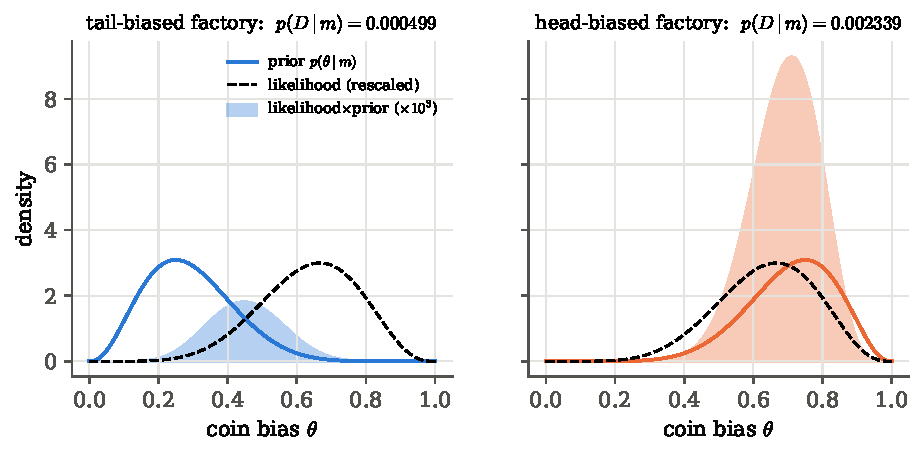
\includegraphics[width=0.95\linewidth]{figures/ch05/factories.pdf}
\caption{The evidence as an area. In each panel the solid curve is the factory's
spread of coin biases (its prior), the dashed curve the likelihood of six heads in
nine tosses (rescaled to fit), and the shaded region their product, whose area is
the evidence printed above the panel. The likelihood is the same in both panels;
only the prior differs, and with it the overlap.}
\label{5c:fig:factories}
\end{figure}

Notice what the comparison did \emph{not} give us: any statement about the bias of
this coin. For that we go back to parameter estimation inside each model. Inside the
tail-biased factory the posterior is $\mathrm{Beta}(z+a,N-z+b)$ with mean
$(z+a)/(N+a+b)=\FiveCFacMeanOne$; inside the head-biased factory the mean is
$\FiveCFacMeanTwo$. If we must give one answer for the bias without deciding on a
factory, we average the two posteriors with the model probabilities as weights,
$\FiveCFacPostOne\%$ and $\FiveCFacPostTwo\%$, which gives the mean $\FiveCFacMeanAvg$
\srcref{Kruschke}{\S10.4}. We return to this averaging in \cref{5c:sec:nested}.

\paragraph{Example: background only, or background plus signal?}
A counter records events from a source that may or may not exist. The background is
well measured: in the time of the run we expect $b=2$ background counts.

\emph{The event.} The run records $n=5$ counts.

\emph{What could have produced it?} Model $M_0$: background only, counts
$\sim\mathrm{Poisson}(b)$. Model $M_1$: background plus a signal of unknown strength
$s$, counts $\sim\mathrm{Poisson}(b+s)$. Before the run, the physics of the source
allows any $s$ between $0$ and $s_{\max}=10$ counts, and we take $s$ uniform in that
range.

\emph{How probable were five counts under each model?} Under $M_0$ there is nothing
to average: $p(n\given M_0)=e^{-b}b^n/n!=\FiveCCntZzero$. Under $M_1$ we average the
Poisson probability over the prior of $s$:
\begin{align}
  p(n\given M_1)
  &\eqby{1}\frac{1}{s_{\max}}\int_0^{s_{\max}}\frac{e^{-(b+s)}(b+s)^n}{n!}\,\dd s
   \eqby{2}\frac{1}{s_{\max}}\int_b^{b+s_{\max}}\frac{e^{-u}u^n}{n!}\,\dd u \nonumber\\
  &\eqby{3}\frac{1}{s_{\max}}\Bigl[F_n(b)-F_n(b+s_{\max})\Bigr],
  \qquad F_n(a)\equiv\sum_{j=0}^{n}\frac{e^{-a}a^j}{j!} .
  \label{5c:eq:counting}
\end{align}
\begin{explain}
  \item The evidence \eqref{5c:eq:evidence} with the uniform prior density
        $1/s_{\max}$.
  \item Substitute $u=b+s$.
  \item The identity $\int_a^\infty e^{-u}u^n/n!\,\dd u=F_n(a)$, the probability that
        a Poisson variable of mean $a$ is at most $n$. It follows by integrating by
        parts $n$ times; each step peels off one term $e^{-a}a^j/j!$. It says that the
        waiting time to the $(n+1)$-th event of a unit-rate Poisson process exceeds
        $a$ exactly when at most $n$ events happened before $a$.
\end{explain}
With $F_5(2)=\FiveCCntCdfb$ and $F_5(12)=\FiveCCntCdfbs$ this gives
$p(n\given M_1)=\FiveCCntZone$ (quadrature agrees). The Bayes factor is
$B_{10}=\FiveCCntB$ in favour of a signal, and with even prior odds the probability
that the source is there is $\FiveCCntPost$.

The Bayes factor is smaller than the best fit would suggest, and the gap is the price
of not knowing $s$. The best signal value is $\hat s=n-b=3$. At that value five
counts are $\FiveCCntLR$ times more probable than under background only. The Bayes
factor is only $\FiveCCntB$. Why? The signal model does not commit to $s=3$. It also
spreads its probability over values like $s=9$, which would have produced far more
than five counts, and those values pull the average down. The ratio of the two
numbers, $\FiveCCntOcc$, is the price the signal model pays for not knowing $s$ in
advance; \cref{5c:sec:occam} derives this price in general. The price depends on how
wide the prior range is. If the physics had allowed anything up to $s_{\max}=100$, the
same five counts would have given $B_{10}=\FiveCCntBWide$, and the data would then
favour background only. The prior range of a parameter is part of what the model
claims.

\begin{keyidea}[The evidence judges a model with its prior]
A model is a likelihood \emph{and} a prior. Its evidence is the likelihood averaged
over its prior, and the Bayes factor, the ratio of two evidences, multiplies the
prior odds of the models. A model that spreads its prior over parameter values the
data do not favour gets a smaller average, even if its best fit is excellent.
\end{keyidea}

Two cautions about reading a quoted Bayes factor. First, conventions differ.
$B_{01}=Z_0/Z_1$ and $B_{10}=Z_1/Z_0=1/B_{01}$ are both in use, and some authors call
$\ln(Z_0/Z_1)$ itself ``the Bayes factor'' \srcref{Padilla}{(13)--(14)}. Always check
which model is in the numerator and whether a logarithm has been taken. Second, a
Bayes factor is not the posterior odds. It multiplies the prior odds, so a model with
prior probability zero stays at zero whatever its Bayes factor
\srcref{Kruschke}{\S10.5.1}.

\subsection{No model is rejected on its own}
\label{5c:sec:alternatives}

Can we ask how probable one model is, without naming any competitor? No. Look at the
denominator of \eqref{5c:eq:model-post}: it is a sum over the competitors, each with
its evidence. Suppose we try to make do with ``$M$ is false'' as the only alternative.
The denominator then needs $p(\data\given\text{not }M)$, the probability of the data
given that $M$ is false. That number cannot be computed, because ``$M$ is false''
makes no prediction for the data \srcref{Sivia}{pp.~87--88}. We need well-defined
alternatives, each making its own prediction. Once we have a list of them, the
question has become model comparison.

A bad fit, on its own, does not make a model improbable. A large $\chi^2$ means a
small likelihood $p(\data\given\params,M)$ at the best parameters. The posterior
probability of $M$ also needs the prior and the evidence of the alternatives, and a
bad fit says nothing about those. What a bad fit does do is tell us to go and look
for an alternative \srcref{Sivia}{p.~88}. The history of Neptune shows that support
for a theory is always support against something \cite[\S4.1]{Trotta2008}. Finding
Neptune near the predicted position strengthened Newtonian gravity against a theory
that predicted no planet there. It did nothing to Newton's standing against
Einstein's gravity, which predicts the same orbit. How much an observation supports a
theory depends on what it is compared with.
\section{Occam's razor from the evidence}
\label{5c:sec:occam}

A better fit alone cannot choose between models. Here is why. Forty measurements
$y_i$ are taken at equally spaced points $x_i$ between $0$ and $10$, each with
Gaussian noise of standard deviation $\sigma=1$. One physicist says the points
scatter about a straight line, $y=a+bx$. A second says there is also a Gaussian bump
on top of the line, the signature of a resonance, with known width $W=0.5$, height $A$
and unknown position $\mu$. Whatever the data, the second physicist's best fit is at
least as good as the first's, because setting $A=0$ turns the bump model into the
line. So the best-fit $\chi^2$ never prefers the simpler model, and a rule that picks
the model with the smallest $\chi^2$ would find a bump in every data set. For the
same reason a tenth-order polynomial always beats a straight line, and nobody believes
it \srcref{Sivia}{p.~81}.

The evidence settles this without any extra rule. The more flexible model spread its
prior over many parameter values, and the data rule most of them out. So its
\emph{average} likelihood, which is the evidence, can be low even when its
\emph{best} likelihood is high.

\subsection{Mr A and Mr B}
\label{5c:sec:mrab}

The simplest version is a story due to Jeffreys, as told by Gull and Sivia
\srcref{Sivia}{\S4.1}. Mr A has a theory with no adjustable parameter. Mr B has a
theory with one adjustable parameter $\lambda$. Whose theory should we prefer, given
data $\data$?

\emph{The event} is the data $\data$. \emph{The hypotheses} are $A$ and $B$.
\emph{How probable was $\data$ under each?} For Mr A this is a straightforward
likelihood, $p(\data\given A)$, since his theory predicts the data with nothing left
to choose. Mr B cannot predict the data without a value of $\lambda$, so his
probability of the data is the evidence \eqref{5c:eq:evidence}, an average over his
prior for $\lambda$. To make it concrete, Sivia makes two simple assumptions
(\cref{5c:fig:mrb}):
\begin{enumerate}[itemsep=1pt,leftmargin=1.6em]
  \item Before seeing the data, Mr B will only say that $\lambda$ lies between
        $\lambda_{\min}$ and $\lambda_{\max}$, so his prior is uniform:
        $p(\lambda\given B)=1/(\lambda_{\max}-\lambda_{\min})$ in that range, zero
        outside \srcref{Sivia}{(4.4)}.
  \item His likelihood has a single peak at the best value $\lambda_0$, of height
        $p(\data\given\lambda_0,B)$, and near the peak it is Gaussian with width
        $\delta\lambda$ \srcref{Sivia}{(4.5)}:
        \[
          p(\data\given\lambda,B)\approx p(\data\given\lambda_0,B)\,
          \exp\!\Bigl[-\frac{(\lambda-\lambda_0)^2}{2\,\delta\lambda^2}\Bigr].
        \]
\end{enumerate}
The likelihood is a function of $\lambda$ but not a density in $\lambda$: its area is
not one. Its height at the peak is the probability of the data at the best value.

\begin{figure}[htbp]
\centering
\begin{tikzpicture}[x=0.9cm,y=3.2cm,font=\small]
  \draw[->,softgray] (0,0) -- (10.6,0) node[right,black] {$\lambda$};
  \draw[->,softgray] (0,0) -- (0,1.18);
  \fill[formblue!15] (1,0) rectangle (9,0.25);
  \draw[form] (1,0) -- (1,0.25) -- (9,0.25) -- (9,0);
  \draw[bdryred,thick,domain=2.5:8.5,samples=120]
    plot (\x,{exp(-(\x-5.5)^2/(2*0.36))});
  \draw[bdryred,dashed,thin] (5.5,0) -- (5.5,1);
  \draw[<->,tangentgreen,thick] (4.9,0.6065) -- (6.1,0.6065);
  \node[tangentgreen!70!black,anchor=west] at (6.25,0.63) {$\pm\delta\lambda$};
  \node[anchor=east] at (0,1) {$p(\data\given\lambda_0,B)$};
  \draw[softgray] (-0.08,1) -- (0.08,1);
  \node[anchor=east] at (0,0.25) {$\dfrac{1}{\lambda_{\max}-\lambda_{\min}}$};
  \draw[softgray] (-0.08,0.25) -- (0.08,0.25);
  \node[below] at (1,0) {$\lambda_{\min}$};
  \node[below] at (9,0) {$\lambda_{\max}$};
  \node[below] at (5.5,0) {$\lambda_0$};
  \node[formblue,anchor=south] at (2.4,0.27) {prior};
  \node[bdryred,anchor=west] at (6.6,0.95) {likelihood};
\end{tikzpicture}
\caption{Mr B's prior and likelihood for his parameter. The prior (blue box) spreads
unit probability evenly over the range $\lambda_{\min}$ to $\lambda_{\max}$; its height
is drawn exaggerated. The likelihood (red) is large only within about $\delta\lambda$ of
its peak. The evidence is the likelihood averaged over the box, so it is roughly the
peak height times the fraction of the box the peak occupies.}
\label{5c:fig:mrb}
\end{figure}

With these two assumptions the average over Mr B's prior can be done by hand:
\begin{align}
  p(\data\given B)
  &\eqby{1}\int p(\data\given\lambda,B)\,p(\lambda\given B)\,\dd\lambda
   \eqby{2}\frac{1}{\lambda_{\max}-\lambda_{\min}}
     \int_{\lambda_{\min}}^{\lambda_{\max}}p(\data\given\lambda,B)\,\dd\lambda \nonumber\\
  &\eqby{3}\frac{p(\data\given\lambda_0,B)}{\lambda_{\max}-\lambda_{\min}}
     \int_{-\infty}^{\infty}e^{-(\lambda-\lambda_0)^2/2\delta\lambda^2}\,\dd\lambda
   \eqby{4}\frac{p(\data\given\lambda_0,B)\;\delta\lambda\sqrt{2\pi}}{\lambda_{\max}-\lambda_{\min}} .
  \label{5c:eq:mrb}
\end{align}
\begin{explain}
  \item The evidence \eqref{5c:eq:evidence} for Mr B.
  \item The uniform prior is a constant inside the range and zero outside, so it comes
        out of the integral and restricts the limits \srcref{Sivia}{(4.6)}.
  \item The Gaussian form of the likelihood. We also assumed the peak lies well inside
        the range, so extending the limits to $\pm\infty$ loses almost nothing.
  \item The Gaussian integral $\int e^{-u^2/2s^2}\dd u=s\sqrt{2\pi}$ \srcref{Sivia}{(4.7)}.
\end{explain}
Put this into the odds \eqref{5c:eq:odds} with $M_1=A$ and $M_2=B$:
\begin{equation}
  \frac{\Prob(A\given\data)}{\Prob(B\given\data)}
  =\underbrace{\frac{\Prob(A)}{\Prob(B)}}_{\text{prior odds}}
   \times\underbrace{\frac{p(\data\given A)}{p(\data\given\lambda_0,B)}}_{\text{best-fit ratio}}
   \times\underbrace{\frac{\lambda_{\max}-\lambda_{\min}}{\delta\lambda\sqrt{2\pi}}}_{\text{Occam factor}} .
  \label{5c:eq:ockham}
\end{equation}
This is Sivia's (4.8). Each of the three factors answers its own question. The first
says what we thought before the data. The second says how well each theory does at
its best; since Mr B can always tune $\lambda$, this ratio can only favour him. The
third is new. It compares the range of $\lambda$ that Mr B's theory allowed before the
data, $\lambda_{\max}-\lambda_{\min}$, with the range the data allow, about
$\delta\lambda$. The first is usually much wider, so this factor is large and favours
Mr A. It is called the
\newterm{Occam factor} (Sivia writes Ockham), because it puts a number on William of
Ockham's rule that ``it is vain to do with more what can be done with fewer''
\srcref{Sivia}{p.~84}.

\begin{workdef}[Occam factor]
For a model with parameters, the \newterm{Occam factor} is the ratio of its evidence
to its best-fit likelihood,
\[
  \frac{Z}{\Like_{\max}}\approx\frac{\text{volume of parameter space allowed by the posterior}}
  {\text{volume allowed by the prior}}\le 1 ,
\]
\unpack{the fraction of the prior's parameter range that the data leave standing}.
The evidence is the best fit times the Occam factor.
\end{workdef}

Reading \eqref{5c:eq:ockham} in a few limits tells us how the razor behaves
\srcref{Sivia}{pp.~84--86}:
\begin{itemize}[itemsep=1pt,leftmargin=1.2em]
  \item \emph{Good data, genuine effect.} If Mr B's extra parameter is really needed,
        the best-fit ratio is tiny (his fit is much better) and it overwhelms the
        Occam factor. Most of the time the goodness of fit decides.
  \item \emph{Good data, no effect.} If Mr B's fit is not much better, the best-fit
        ratio stays near one, while more data make $\delta\lambda$ smaller and the Occam
        factor larger. Mr A is favoured ever more strongly as the data improve.
  \item \emph{Poor data.} If the data barely constrain $\lambda$, then $\delta\lambda$
        approaches the prior range and the likelihood is flat, so both the best-fit
        ratio and the Occam factor approach one. The posterior odds return to the
        prior odds: poor data have taught us nothing.
  \item \emph{Unbounded prior.} If $\lambda_{\max}-\lambda_{\min}\to\infty$, the Occam
        factor is infinite and Mr B always loses. Jeffreys worried about this. In
        practice the range is always bounded by what we know. A new fifth force with
        a huge coupling would have been noticed long ago, so its strength has an upper
        bound before any new experiment.
\end{itemize}

Two variations make the razor sharper.
\begin{itemize}[itemsep=1pt,leftmargin=1.2em]
  \item \emph{Both theories have one parameter.} Give Mr A a parameter $\mu$, with a
        uniform prior and a Gaussian likelihood of width $\delta\mu$, just like Mr B's.
        Each evidence now carries its own Occam factor. With equal prior ranges the
        ranges cancel, and the posterior odds are the best-fit ratio times
        $\delta\mu/\delta\lambda$ \srcref{Sivia}{(4.9)}. So for equally good fits the
        theory with the \emph{larger} error bar wins. That sounds backwards, but a
        larger error bar means that more of the theory's parameter values agree with
        the data.
  \item \emph{The same theory, two prior ranges.} Let Mr A and Mr B hold the same
        theory, but let Mr A claim a narrower prior range, still wide enough to
        contain the fit. Everything cancels except the ranges, and the odds are the
        ratio of the ranges in Mr A's favour. He predicted the parameter more
        precisely, and the evidence rewards him for it.
\end{itemize}

None of this touches parameter estimation. Inside Mr B's theory the posterior for
$\lambda$ is likelihood times prior divided by the evidence \srcref{Sivia}{(4.10)}.
The prior is the constant $1/(\lambda_{\max}-\lambda_{\min})$, and it appears in both
the numerator and the evidence \eqref{5c:eq:mrb}, so it cancels; so does the peak
height. What is left is the Gaussian $\lambda=\lambda_0\pm\delta\lambda$, whatever the
range, as long as the range contains the peak. The range matters only when we compare
models. The same equation serves both purposes; we are asking it different questions.

\paragraph{Example: the counting experiment again.}
In \cref{5c:sec:bf} five counts on an expected background of $b=2$ gave a best-fit
likelihood ratio of $\FiveCCntLR$ for a signal, but a Bayes factor of only
$\FiveCCntB$. The Occam factor explains the difference. We need the width $\delta s$ of
the likelihood. The log-likelihood is $\ln p(n\given s)=-(b+s)+n\ln(b+s)-\ln n!$. Its
second derivative is $-n/(b+s)^2$, and at the peak $\hat s=n-b$, where $b+s=n$, this
is $-1/n$. A Gaussian of width $\delta s$ has second derivative of its logarithm
$-1/\delta s^2$, so $\delta s=\sqrt n=\sqrt5$. The prior range is $s_{\max}=10$, and
\eqref{5c:eq:mrb} gives the Occam factor
\[
  \frac{\delta s\sqrt{2\pi}}{s_{\max}}=\frac{\sqrt{10\pi}}{10}\approx0.56 ,
\]
close to the exact ratio $\FiveCCntOcc$ of evidence to best fit. The Gaussian
approximation is rough for a Poisson likelihood with five counts, but the size of the
penalty is right: a signal prior of width $10$ against a data width of about $2.2$.

\paragraph{Example: must be fair, or anything goes?}
Kruschke's version compares two coin factories that differ only in how widely they
spread their coin biases \srcref{Kruschke}{\S10.5}. The ``must-be-fair'' factory makes
coins with $\theta\sim\mathrm{Beta}(500,500)$, all very close to $0.5$. The
``anything-goes'' factory makes $\theta\sim\mathrm{Beta}(1,1)$, uniform on $[0,1]$. The
second model is the more flexible: it contains a coin matching any observed fraction of
heads. The evidence of each is \eqref{5c:eq:beta-evidence}. For $z=15$ heads in $N=20$
tosses the Bayes factor of fair against anything is $\FiveCFairFifteen$: the fair model
has no bias near $0.75$, and loses. For $z=11$ heads it is $\FiveCFairEleven$: now the
fair model wins, although the anything model contains the bias $0.55$ that matches the
data exactly. The anything model pays for spreading its prior over biases like $0.1$
and $0.9$ that these data rule out. \Cref{5c:fig:fair} shows the pattern for every
possible $z$: the simpler model wins whenever the data are consistent with it, here for
$\FiveCFairZmin\le z\le\FiveCFairZmax$.

\begin{figure}[htbp]
\centering
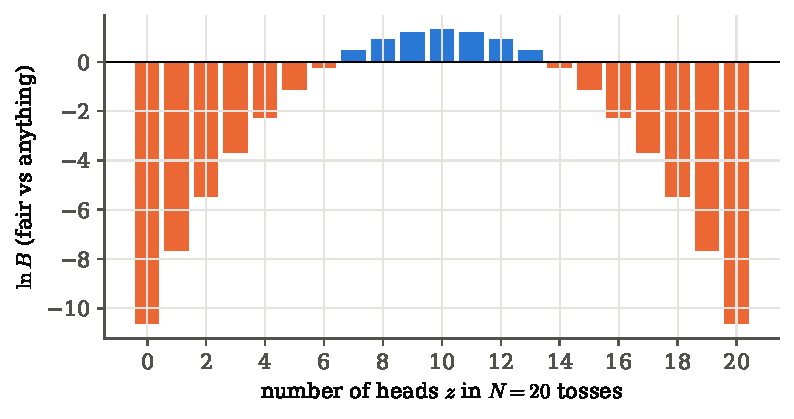
\includegraphics[width=0.78\linewidth]{figures/ch05/fair_vs_anything.pdf}
\caption{Natural Occam's razor for coins. For each possible number of heads in twenty
tosses, the bar is the log Bayes factor of the must-be-fair factory against the
anything-goes factory. Near ten heads the simple model wins by a modest factor (blue);
far from ten it loses by a large one (orange), because it simply cannot produce such
data.}
\label{5c:fig:fair}
\end{figure}

The picture is asymmetric, and that is typical. A simple model that is wrong is
punished hard, because it has no parameter value near the data. A flexible model that
is unnecessary is punished gently, by a factor of a few, the size of its Occam factor.

\subsection{Many parameters: the Laplace approximation}
\label{5c:sec:laplace-evidence}

The same argument works in $D$ dimensions. Near its peak $\hat\params$ the logarithm
of the likelihood is approximately quadratic,
\[
  \ln\Like(\params)\approx\ln\Like_{\max}-\tfrac12(\params-\hat\params)\T\Fish\,(\params-\hat\params),
\]
where $\Fish$ is the matrix of second derivatives of $-\ln\Like$ at the peak
\unpack{the curvature of the log-likelihood, the Fisher matrix of \cref{ch:10}
evaluated on these data}. Its inverse is the covariance of the Gaussian approximation
to the posterior. If the prior $\pi(\params)$ changes little across the peak,
\begin{align}
  Z
  &\eqby{1}\int\Like(\params)\,\pi(\params)\,\dd^D\params
   \relby{2}{\approx}\Like_{\max}\,\pi(\hat\params)
     \int e^{-\frac12(\params-\hat\params)\T\Fish(\params-\hat\params)}\,\dd^D\params \nonumber\\
  &\eqby{3}\Like_{\max}\,\pi(\hat\params)\,\frac{(2\pi)^{D/2}}{\sqrt{\det\Fish}}
   \eqby{4}\Like_{\max}\times\frac{(2\pi)^{D/2}\sqrt{\det\Cmat}}{V_\pi} .
  \label{5c:eq:laplace-evidence}
\end{align}
\begin{explain}
  \item The evidence, with $\Like(\params)=p(\data\given\params,M)$ and
        $\pi(\params)=p(\params\given M)$.
  \item The quadratic expansion of $\ln\Like$, and the prior taken out at the peak.
  \item The $D$-dimensional Gaussian integral. Rotate to the eigenvectors of the
        symmetric positive matrix $\Fish$; the integral factorises into $D$
        one-dimensional integrals $\sqrt{2\pi/f_k}$, one per eigenvalue $f_k$, and the
        product of the eigenvalues is $\det\Fish$.
  \item For a uniform prior on a region of volume $V_\pi$, $\pi(\hat\params)=1/V_\pi$;
        and $\Cmat=\Fish^{-1}$, so $1/\sqrt{\det\Fish}=\sqrt{\det\Cmat}$.
\end{explain}
This is the \newterm{Laplace approximation} to the evidence
\srcref{Sivia}{(4.20)}, \cite[eqs.~(24)--(25)]{Trotta2008}. The factor
$(2\pi)^{D/2}\sqrt{\det\Cmat}$ is the volume of the posterior's ``error ellipsoid'',
so the Occam factor of \eqref{5c:eq:ockham} generalises to the ratio of the posterior
volume to the prior volume. In one dimension it is $\sqrt{2\pi}\,\delta\lambda$ over
$\lambda_{\max}-\lambda_{\min}$ again.

\begin{keyidea}[Evidence $\approx$ best fit $\times$ Occam factor]
\[
  Z\;\approx\;\Like_{\max}\times\frac{V_{\rm posterior}}{V_{\rm prior}} .
\]
A model is rewarded for fitting the data well and penalised by the fraction of its
prior parameter space that the data rule out. Every parameter the data constrain adds
a factor $\sqrt{2\pi}\,\sigma_k/(\text{prior range}_k)$ (for uncorrelated parameters); a model is favoured only if its
better fit pays for all of them.
\end{keyidea}

Two remarks keep the formula honest. First, a parameter the data do not constrain at
all has a posterior as wide as its prior, contributes a factor one, and costs nothing.
Adding the price of fish at Billingsgate market to a cosmological model changes no
prediction, so the likelihood is flat in it and the evidence is unchanged however wide
its prior \srcref{HobsonBMC}{p.~85}, \cite[p.~16]{Trotta2008}. What the evidence
penalises is not the number of parameters but wasted predictive range: parameter
values the model allowed and the data rule out. Hobson and collaborators put it as
``the Bayesian evidence rewards model predictiveness'' \srcref{HobsonBMC}{p.~83}.
Second, if the likelihood has several separate peaks, each contributes its own
term. With $M$ identical bumps whose labels can be permuted, the likelihood has $M!$
equivalent peaks and the Laplace sum must count all of them \srcref{Sivia}{(4.20)}.
An exact integral over the whole prior box counts them automatically.

\subsection{A line, or a line plus a bump?}
\label{5c:sec:bump}

Back to the forty points. The two models are
\begin{align*}
  M_0\ (\text{line}):\quad & y_i=a+bx_i+\epsilon_i,\\
  M_1\ (\text{line}+\text{bump}):\quad & y_i=a+bx_i+A\,e^{-(x_i-\mu)^2/2W^2}+\epsilon_i,
  \qquad\epsilon_i\iid\Normal(0,1),
\end{align*}
with the bump width $W=\FiveCWidth$ known. The priors are part of the models and are
fixed before looking at the data: $a$ uniform on $[0,20]$ and $b$ uniform on $[-2,2]$
in both models; in $M_1$ also $A$ uniform on $[0,A_{\max}]$ with
$A_{\max}=\FiveCAmax$ (a generous ceiling, ten times the noise) and $\mu$ uniform
on $[0,10]$ (the range we measured). We simulate two data sets, one with a real bump of
height $\FiveCTrueA$ at $\mu=\FiveCTrueMu$ and one with no bump, both on the line
$y=5+0.3x$ (\cref{5c:fig:bump-fits}).

\begin{figure}[htbp]
\centering
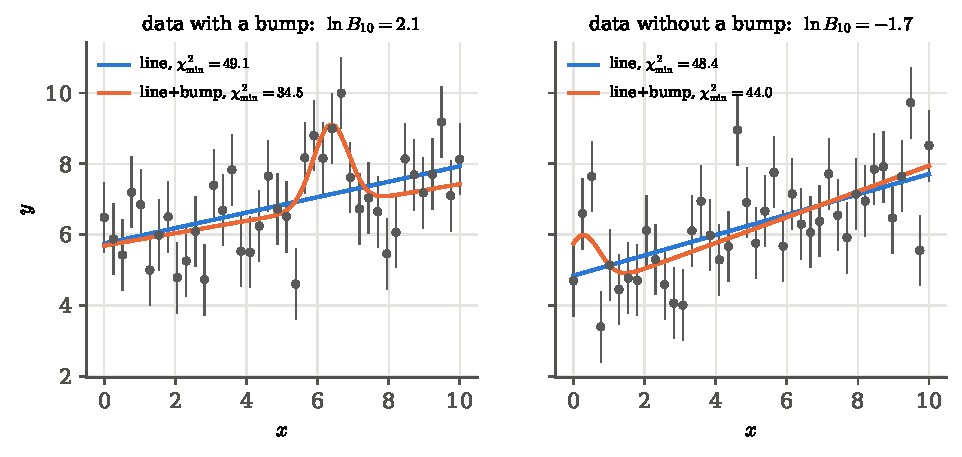
\includegraphics[width=\linewidth]{figures/ch05/line_bump_fits.pdf}
\caption{Two simulated data sets of forty points with unit error bars, and the best fits
of both models. Left: a bump of height $2.5$ is present near $x=6.2$; the bump model
finds it and its $\chi^2$ drops by $\FiveCBumpDChi$. Right: there is no bump; the bump
model still finds a small improvement by fitting a noise fluctuation. The log Bayes
factor of bump against line is printed above each panel.}
\label{5c:fig:bump-fits}
\end{figure}

\paragraph{Integrating out the line exactly.}
The evidence of $M_1$ is a four-dimensional integral over $(a,b,A,\mu)$. The line
parameters $a,b$ enter the model linearly, so the likelihood is Gaussian in them and
their integral can be done exactly. That leaves a two-dimensional integral over
$(A,\mu)$ for the grid. The question for each bump is: once the bump $(A,\mu)$ is
subtracted, how well can the best line fit what remains? Write the data as the vector
$\bm y$ (here $N=40$), the two line shapes as the columns of the $N\times2$ matrix
$X=(\bm1,\bm x)$, and the bump shape at position $\mu$ as the vector $\bm g_\mu$. For
fixed $(A,\mu)$ the line fits $\bm y-A\bm g_\mu$. What it cannot fit is the part of
$\bm y-A\bm g_\mu$ that points in directions no line can reach,
$P_\perp(\bm y-A\bm g_\mu)$, where $P_\perp=\Id-X(X\T X)^{-1}X\T$ is the projector onto
those directions. Writing $\bm r=P_\perp\bm y$ and $\bm u_\mu=P_\perp\bm g_\mu$,
\begin{align}
  \chi^2_{\min}(A,\mu)-\chi^2_{\min,\rm line}
  &\eqby{1}\lVert\bm r-A\bm u_\mu\rVert^2-\lVert\bm r\rVert^2
   \eqby{2}-2A\,\bm r\cdot\bm u_\mu+A^2\,\bm u_\mu\cdot\bm u_\mu .
  \label{5c:eq:dchi2}
\end{align}
\begin{explain}
  \item With $\sigma=1$, the minimum of $\chi^2$ over the line is the squared length of
        the residual the line cannot absorb; for the line model alone that residual is
        $\bm r$.
  \item Expand the square: $\lVert\bm r-A\bm u\rVert^2=\lVert\bm r\rVert^2-2A\,\bm r\cdot\bm u+A^2\lVert\bm u\rVert^2$.
\end{explain}
The integral over $(a,b)$ at fixed $(A,\mu)$ is the same Gaussian integral in both
models, because both use the same line shapes and the same prior box for the line. It
cancels in the Bayes factor, which is therefore
\begin{equation}
  B_{10}=\frac{1}{A_{\max}\cdot10}\int_0^{A_{\max}}\!\!\int_0^{10}
  \exp\!\Bigl[-\tfrac12\bigl(\chi^2_{\min}(A,\mu)-\chi^2_{\min,\rm line}\bigr)\Bigr]\,\dd\mu\,\dd A .
  \label{5c:eq:bump-bf}
\end{equation}
In words: the likelihood ratio of each bump to the best line, averaged over the prior
box of bumps. (We assumed that the line's prior box is wide enough to contain its
likelihood; with the boxes above it is, by many standard deviations.)

\pyfile[firstline=72,lastline=91,firstnumber=72]{code/ch05/lib_bump.py}{The Bayes
factor of bump against line on a grid}

Lines 74--78 build \eqref{5c:eq:dchi2} for every $(A,\mu)$ on the grid at once: the
projected data $\bm r$, the projected bump shapes $\bm u_\mu$ (one column per
position), their dot products, and the quadratic in $A$. Line 86 exponentiates to get
the likelihood ratio to the best line; lines 87--88 average it over $\mu$ and then over
$A$ with the trapezoid rule, which is \eqref{5c:eq:bump-bf}. Working with the ratio to
the best line keeps the numbers of order one; the raw likelihoods are about $e^{-60}$.

\paragraph{The data with a bump.}
The line has $\chi^2_{\min}=\FiveCBumpChiLine$ for $38$ degrees of freedom, the bump
model $\FiveCBumpChiBump$ at $\hat A=\FiveCBumpAhat$, $\hat\mu=\FiveCBumpMuhat$. The best
bump improves the fit by $\Delta\chi^2=\FiveCBumpDChi$, a best-fit likelihood ratio of
$e^{\FiveCBumplnLR}$. The Bayes factor is $\ln B_{10}=\FiveCBumplnB$ ($B_{10}=\FiveCBumpB$;
a grid of half the resolution changes $\ln B_{10}$ by $\FiveCBumpGridErr$). The
difference, $\ln B_{10}-\tfrac12\Delta\chi^2=\FiveCBumplnOccam$, is the logarithm of the
Occam factor. Here the bump is favoured, but by odds of $\FiveCBumpB$ to $1$, not by the
$e^{\FiveCBumplnLR}$ that the fit improvement alone suggests.

The Laplace approximation \eqref{5c:eq:laplace-evidence} lets us read the Occam factor
off the map of \cref{5c:fig:bump-map}. At the best fit the posterior standard deviations
are $\sigma_A=\FiveCSigA$ and $\sigma_\mu=\FiveCSigMu$, so the posterior area in the
$(A,\mu)$ plane is $2\pi\sqrt{\det\Cmat_{A\mu}}=\FiveCSigAMuVol$, against a prior area of
$A_{\max}\times10=\FiveCPriorAMuVol$. Their ratio, $\FiveCLapOccRatio$, is the Occam
factor, and the Laplace estimate of the Bayes factor is $\ln B_{10}=\FiveCLapLnB$,
close to the exact $\FiveCBumplnB$. The bump model allowed $\FiveCPriorAMuVol$ square
units of bumps and the data kept only $\FiveCSigAMuVol$ of them.

\begin{figure}[htbp]
\centering
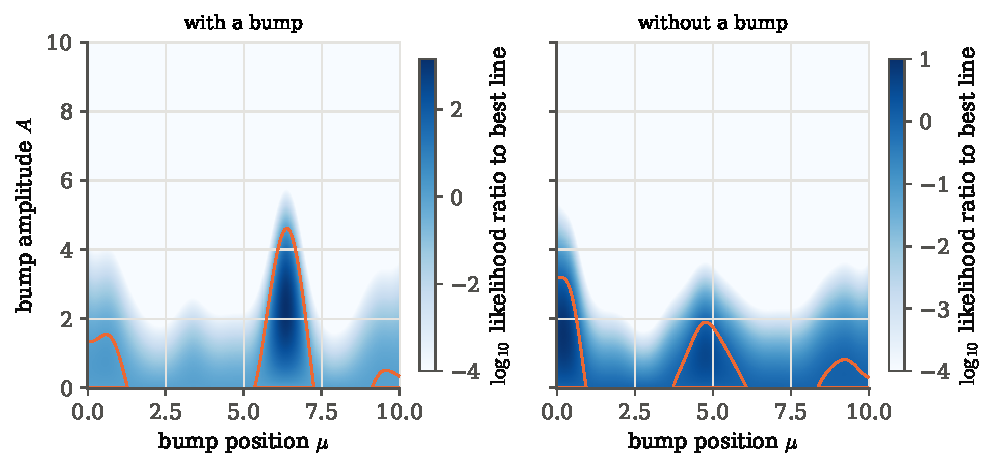
\includegraphics[width=\linewidth]{figures/ch05/line_bump_map.pdf}
\caption{The likelihood of every bump in the prior box, relative to the best line, in
powers of ten. With a bump in the data (left) a small island near
$\mu=\FiveCBumpMuhat$, $A=\FiveCBumpAhat$ is
far better than the line; almost all the rest of the box is worse. Without a bump
(right) nothing is much better than the line. The orange contour marks a likelihood
ratio of one. The Bayes factor is the average of this map over the box.}
\label{5c:fig:bump-map}
\end{figure}

\paragraph{The data without a bump.}
Here the bump model still finds something: a noise fluctuation at
$\hat\mu=\FiveCFlatMuhat$ improves $\chi^2$ from $\FiveCFlatChiLine$ to
$\FiveCFlatChiBump$. A $\chi^2$ drop of a few units for two extra parameters is what
noise does. The evidence agrees: $\ln B_{10}=\FiveCFlatlnB$, so the line is favoured by
a factor $1/\FiveCFlatB$. The Occam factor, $e^{\FiveCFlatlnOccam}$, outweighs the
modest improvement of the fit. For both data sets the razor cuts in the right
direction, and it needed no rule beyond the sum and product rules.

\paragraph{If we had known where to look.}
Not knowing where the bump sits has a price, and the evidence charges it
automatically. Suppose theory had predicted the resonance at $\mu=\FiveCTrueMu$, so
that $M_1$ has only the amplitude free. Then the prior no longer wastes probability on
positions the data rule out. For the data with a bump, $\ln B_{10}=\FiveCFixLnB$
($B_{10}=\FiveCFixB$), which is $\FiveCFreeOverFix$ times larger than with the position
free. At the predicted position the amplitude is $\FiveCFixAhat\pm\FiveCFixSigA$, a
local significance of $\FiveCFixZscore\sigma$. So not knowing the position costs a
factor of $\FiveCFreeOverFix$. This is the look-elsewhere effect of \cref{ch:04}. There it
needed a separate trials factor; here it appears by itself, as the Occam factor of the
parameter $\mu$.
\section{Reading a Bayes factor}
\label{5c:sec:reading}

With three years of WMAP data and the large-scale-structure surveys of the time, a
cosmological model with a free spectral index $n_s$ was found to have a log evidence
$1.99\pm0.26$ higher than the Harrison--Zel'dovich model with $n_s=1$
\srcref{HobsonBMC}{Table~4.4}. The same data gave $n_s=0.958\pm0.016$, nearly three
standard deviations from one. How impressed should we be by $\ln B=2$? Is it the same
statement as ``three sigma'', the significance of \cref{ch:04}? And would another
reasonable choice of prior have given a different number?

\subsection{The Jeffreys scale}
\label{5c:sec:jeffreys}

A Bayes factor multiplies the prior odds. With even prior odds and only two models,
the posterior probability of the favoured model is
\begin{equation}
  \Prob(M_1\given\data)=\frac{B_{10}}{1+B_{10}},
  \qquad\text{e.g.}\quad
  B_{10}=e^{1}\approx2.7\ \to\ 0.73,\quad
  e^{2.5}\approx12\ \to\ 0.92,\quad
  e^{5}\approx150\ \to\ 0.993 ,
  \label{5c:eq:bf-prob}
\end{equation}
from \eqref{5c:eq:odds} with $\Prob(M_1)=\Prob(M_0)$ and $\Prob(M_1\given\data)+\Prob(M_0\given\data)=1$.
Jeffreys proposed words for these levels, and a version of his scale is quoted in
almost every cosmology paper that computes an evidence
\srcref{HobsonBMC}{\S4.5}, \srcref{Padilla}{Table~II}, \cite[Table~1]{Trotta2008},
\cite{KassRaftery1995}:

\begin{center}
\small
\renewcommand{\arraystretch}{1.15}
\begin{tabular}{@{}cccp{2.6cm}p{1.6cm}p{1.6cm}@{}}
\toprule
$\lvert\ln B\rvert$ & odds & probability & Jeffreys & Hobson et al. & Trotta \\\midrule
$<1$ & $<3:1$ & $<0.75$ & not worth more than a bare mention & --- & inconclusive\\
$1$--$2.5$ & $3:1$ to $12:1$ & $0.75$--$0.92$ & significant & weak & weak\\
$2.5$--$5$ & $12:1$ to $150:1$ & $0.92$--$0.993$ & strong to very strong & significant & moderate\\
$>5$ & $>150:1$ & $>0.993$ & decisive & strong & strong\\
\bottomrule
\end{tabular}
\end{center}

\noindent The probability column assumes even prior odds and two models, and the table
rounds $e^{1}\approx2.7$ up to $3:1$. The
thresholds are a convention, calibrated on experience, not a theorem. Three cautions
come with them.
\begin{itemize}[itemsep=1pt,leftmargin=1.2em]
  \item \emph{The scale is logarithmic.} Moving up one level needs roughly ten times
        more support. Evidence accumulates slowly \cite[p.~14]{Trotta2008}.
  \item \emph{It applies to posterior odds.} The words are meant for the ratio of
        posterior model probabilities; they coincide with the Bayes factor only when
        the prior odds are even \srcref{HobsonBMC}{p.~90}. A Bayes factor of $20$
        for an exotic model that we believed at $1:1000$ beforehand still leaves it at
        $1:50$.
  \item \emph{The priors are uncertain too.} Because a Bayes factor depends on the
        prior widths (\cref{5c:sec:prior-width}), Hobson and collaborators soften
        Jeffreys' words: $\ln B$ between $1$ and $2.5$ is only ``weak'', between $2.5$ and
        $5$ ``significant'', above $5$ ``strong'' (third column of the table) \srcref{HobsonBMC}{p.~90}.
        Trotta's column is similar. Kruschke's rule of thumb, ``substantial'' above $B=3$,
        is the same first threshold \srcref{Kruschke}{p.~268}.
\end{itemize}
An evidence computed numerically also has an error, like $\pm0.26$ above, and a
difference in $\ln B$ smaller than its error means nothing.

\paragraph{Example: is the primordial spectrum tilted?}
The two models are the tilted one ($n_s$ free) and Harrison--Zel'dovich ($n_s=1$). In
the WMAP analysis \srcref{HobsonBMC}{pp.~91--93} the log Bayes factor of tilted
against Harrison--Zel'dovich grew as the data improved:
\begin{itemize}[itemsep=1pt,leftmargin=1.2em]
  \item first-year WMAP with other data: $\ln B=-0.58\pm0.12$, inconclusive, with a
        slight preference for the simpler model;
  \item three-year WMAP alone: $0.34\pm0.26$, still inconclusive;
  \item three-year WMAP with other data: $1.99\pm0.26$, odds of about $7:1$,
        ``significant'' in Jeffreys' words and ``weak'' in the softer scale.
\end{itemize}
Then inflation was taken seriously. Slow roll predicts a tilt \emph{and} a
tensor-to-scalar ratio $r$, so this model has two new parameters. Its verdict depended
on the prior for $r$. With $r$ uniform between $0$ and $1$, the $n_s$--$r$ model came
out at $\ln B=-1.45\pm0.45$, disfavoured against Harrison--Zel'dovich. With $\ln r$
uniform from $-80$ to $0$ it came out at $1.90\pm0.24$, about as good as the
$n_s$-only model. The data were identical. Why did the prior on $r$ matter so much?
The data allow only small $r$. A uniform prior on $[0,1]$ puts most of its weight on
larger values of $r$, which the data exclude, so it pays an Occam factor. The
logarithmic prior puts most of its weight on tiny $r$, which the data cannot
distinguish from zero. There the likelihood is flat, so this prior pays almost
nothing: this is the Billingsgate effect of \cref{5c:sec:laplace-evidence}.

\subsection{The prior width sets the price}
\label{5c:sec:prior-width}

The wider the prior range of an extra parameter, the less the data favour it. The
reason is the Occam factor of \eqref{5c:eq:ockham}: it is the data's range divided by
the prior range. So once the prior range is much wider than the likelihood, the Bayes
factor in favour of the extra parameter falls in proportion to the range: every factor
of ten in the range subtracts $\ln10\approx2.3$ from $\ln B_{10}$. Take the bump of
\cref{5c:sec:bump} and vary only the prior range $A_{\max}$ of its amplitude
(\cref{5c:fig:width}). For the data with a bump, $\ln B_{10}$ first rises, because a
prior that stops below the fitted amplitude $\hat A=\FiveCBumpAhat$ cannot reach the
bump; it peaks once the range just covers it; then it falls along a straight line of
slope $-1$ in $\ln A_{\max}$. At $A_{\max}=100$ it is $\FiveCBumpLnBHundred$, against
$\FiveCBumplnB$ at $A_{\max}=10$: the same bump, with the same local significance of
$\FiveCFixZscore\sigma$, is now worth ten times less evidence. For the data
without a bump $\ln B_{10}$ starts at zero (for a tiny range the two models are the
same model) and falls steadily, reaching $\FiveCFlatLnBHundred$ at $A_{\max}=100$.

\begin{figure}[htbp]
\centering
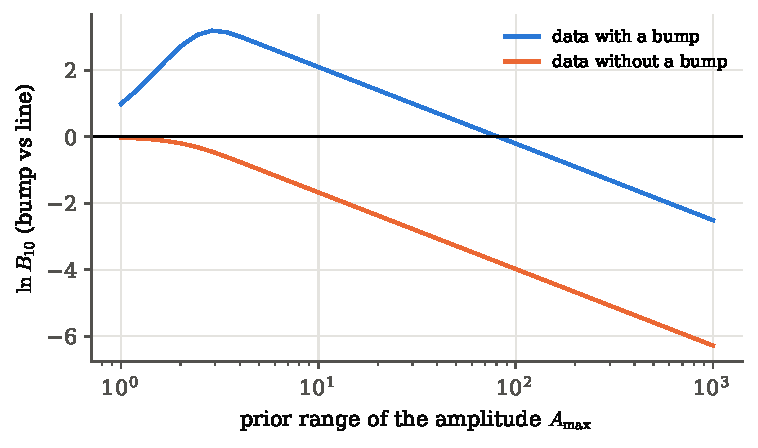
\includegraphics[width=0.75\linewidth]{figures/ch05/line_bump_width.pdf}
\caption{The Bayes factor of bump against line as the prior range of the bump amplitude
is widened, for the two data sets of \cref{5c:fig:bump-fits}. Past the fitted amplitude
both curves fall by $\ln 10$ per decade of $A_{\max}$: each widening of the prior
spreads the model's probability over more bumps the data rule out.}
\label{5c:fig:width}
\end{figure}

So which range is right? The answer has to come from physics, before the data: the
largest resonance the experiment would already have noticed, the range of $n_s$ that
slow-roll inflation allows ($0.8\lesssim n_s\lesssim1.2$), the coupling a fifth force
could have without being seen \srcref{Sivia}{p.~85}, \cite[\S4.5]{Trotta2008}. If
several plausible ranges give the same qualitative verdict, the verdict is robust. If
not, the honest report is the Bayes factor as a function of the range, which is what
\cref{5c:fig:width} is. In the $(\text{information},\text{significance})$ plane of
\cref{5c:sec:lindley} a change of prior width is a horizontal shift
\cite[\S4.4]{Trotta2008}.

\paragraph{Example: two vague priors, one posterior, two verdicts.}
Two priors that both claim to know nothing can give opposite verdicts
\srcref{Kruschke}{\S10.6}. A coin gives $z=65$ heads in $N=100$ tosses. Model one is
must-be-fair, $\theta\sim\mathrm{Beta}(500,500)$, where $\theta$ is the probability of
heads. Model two is anything-goes, and we must choose a vague prior for it.
\begin{itemize}[itemsep=1pt,leftmargin=1.2em]
  \item With $\mathrm{Beta}(1,1)$, uniform, the Bayes factor of fair against anything
        is $\FiveCHalUnifBF$: anything-goes wins by $8:1$.
  \item With the Haldane prior $\mathrm{Beta}(0.01,0.01)$, recommended by some
        statisticians as maximally uninformative, the Bayes factor is
        $\FiveCHalHaldBF$: must-be-fair wins by nearly $6:1$.
\end{itemize}
The verdict reversed. Yet the posteriors of $\theta$ under the two vague priors are
practically the same: their $95\%$ HDIs are $[\FiveCHdiUnifLo,\FiveCHdiUnifHi]$ and
$[\FiveCHdiHaldLo,\FiveCHdiHaldHi]$, and both exclude $0.5$. How can the posterior stay
put while the evidence flips? The evidence \eqref{5c:eq:evidence} is the likelihood
averaged over the prior. The Haldane prior puts almost all its probability extremely
close to $\theta=0$ and $\theta=1$. So its density near $\theta=0.65$, where the
likelihood lives, is tiny, and the average of the likelihood over the prior is tiny
with it. The posterior, by contrast, is renormalised: it does not care about the
overall level of the prior near $0.65$, only about its shape there, and there both
priors are nearly flat.

Lambert shows the same thing for a binomial sample \srcref{Lambert}{\S10.6,
Fig.~10.12}: fifteen counts, each out of ten trials, with a $\mathrm{Beta}(a,a)$ prior
on the success probability (\cref{5c:fig:prior-sens}). As $a$ goes from $0.01$ to $1$
to $10$ the posterior hardly moves (mean $\FiveCLamMeanA$, standard deviation
$\FiveCLamSdA$ against $\FiveCLamSdB$), while $\ln p(\data)$ goes from $\FiveCLamLnZa$ to
$\FiveCLamLnZb$ to $\FiveCLamLnZc$: a factor $\FiveCLamZratio$ in the evidence between the
first two ``vague'' choices.

\begin{figure}[htbp]
\centering
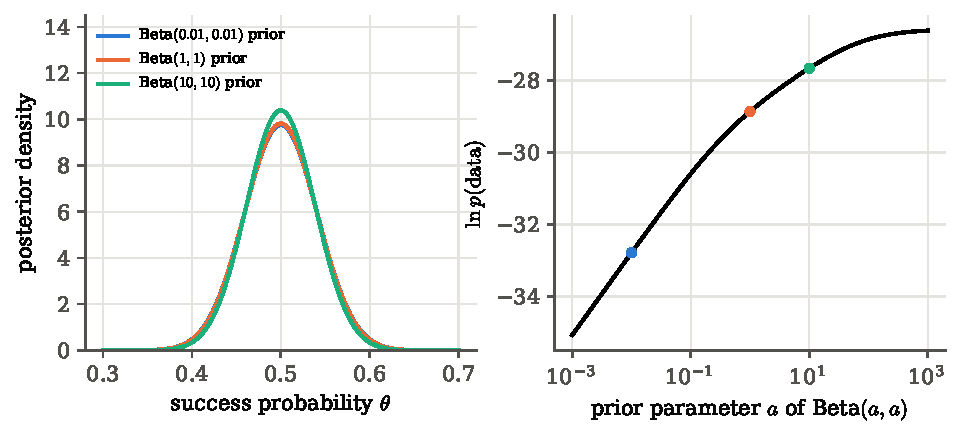
\includegraphics[width=\linewidth]{figures/ch05/prior_sensitivity.pdf}
\caption{Left: the posterior of a success probability under three symmetric Beta
priors, for fifteen binomial counts out of ten trials each; the three curves nearly
coincide. Right: the log evidence of the same data as a function of the prior
parameter $a$; the three dots are the three priors on the left. The posterior barely
notices the prior, the evidence notices it a lot.}
\label{5c:fig:prior-sens}
\end{figure}

Kruschke's remedy is to put the competing models on an equal footing: inform the priors
of \emph{both} models with the same small, representative part of the data, and compute
the Bayes factor from the rest \srcref{Kruschke}{\S10.6.1}. Why does this help? Even a
few data points overwhelm a vague prior and bring each model's parameters ``into the
ballpark'', so the arbitrary choice of vague prior no longer matters. For the
coin, use $6$ heads in the first $10$ tosses to update both priors, then compare on the
remaining $90$. The Bayes factor of fair against anything becomes $\FiveCInfUnifBF$ starting
from the uniform prior and $\FiveCInfHaldBF$ starting from the Haldane prior. The two vague
priors now agree, and both say the coin is not fair, as the HDIs did. Intrinsic and
fractional Bayes factors are more systematic versions of the same idea.

\begin{pitfall}[Vague priors are harmless for estimation, not for comparison]
A wide or ``uninformative'' prior is usually safe when estimating a parameter,
because the likelihood dominates the posterior. In model comparison the overall height
of the prior where the likelihood lives enters directly, and changing from one vague
prior to another can change the Bayes factor by orders of magnitude. An improper prior,
one that cannot be normalised (flat on the whole real line), gives an evidence with an
arbitrary constant in it, so Bayes factors with improper priors on the extra parameters
are undefined \mainref{p.~185}, \srcref{HobsonBMC}{\S1.3}.
\end{pitfall}

\subsection{Lindley's paradox}
\label{5c:sec:lindley}

The simplest nested comparison can be done exactly, and it holds a surprise. We have a
measurement $\hat\theta$ of a quantity $\theta$ with Gaussian error $\sigma$. Model
$M_0$ says the effect is absent, $\theta=0$. Model $M_1$ says it is present, with a
size we can only bound: $\theta\sim\Normal(0,\Sigma^2)$ with $\Sigma$ the scale of
effects the theory allows. Call $\lambda=\lvert\hat\theta\rvert/\sigma$ the
significance of the measurement, the ``number of sigma''.

\emph{The event:} the value $\hat\theta$. \emph{The hypotheses:} $M_0$ and $M_1$.
\emph{How probable was $\hat\theta$ under each?} Under $M_0$ it is the Gaussian density
$\Normal(\hat\theta;0,\sigma^2)$. Under $M_1$ we average over $\theta$:
\begin{align}
  p(\hat\theta\given M_1)
  &\eqby{1}\int\Normal(\hat\theta;\theta,\sigma^2)\,\Normal(\theta;0,\Sigma^2)\,\dd\theta
   \eqby{2}\Normal(\hat\theta;0,\sigma^2+\Sigma^2), \nonumber\\
  B_{01}=\frac{p(\hat\theta\given M_0)}{p(\hat\theta\given M_1)}
  &\eqby{3}\sqrt{\frac{\sigma^2+\Sigma^2}{\sigma^2}}\,
     \exp\!\Bigl[-\frac{\hat\theta^2}{2\sigma^2}+\frac{\hat\theta^2}{2(\sigma^2+\Sigma^2)}\Bigr]
   \eqby{4}\sqrt{1+\frac{\Sigma^2}{\sigma^2}}\,
     \exp\!\Bigl[-\frac{\lambda^2}{2}\,\frac{\Sigma^2}{\sigma^2+\Sigma^2}\Bigr] .
  \label{5c:eq:gauss-bf}
\end{align}
\begin{explain}
  \item The evidence of $M_1$: the likelihood of the measurement averaged over the
        prior of the effect.
  \item The measurement is the true effect plus independent Gaussian noise, so it is
        a sum of two independent Gaussians of variances $\Sigma^2$ and $\sigma^2$, and
        its density is the Gaussian of the summed variance (the convolution of two
        Gaussians; complete the square in $\theta$ to check).
  \item Ratio of the two Gaussian densities: the prefactors give the square root, the
        exponents subtract.
  \item Combine the exponents over the common denominator and write
        $\hat\theta^2/\sigma^2=\lambda^2$.
\end{explain}
This is Trotta's (21) \cite[p.~13]{Trotta2008}. When the data are much more precise than
the prior, $\sigma\ll\Sigma$, the last factor becomes $e^{-\lambda^2/2}$ and
\begin{equation}
  \ln B_{01}\approx\ln\frac{\Sigma}{\sigma}-\frac{\lambda^2}{2}
  \label{5c:eq:rough-guide}
\end{equation}
\cite[eq.~(26)]{Trotta2008}: the Occam term $\ln(\Sigma/\sigma)$, the logarithm of the
ratio of prior to posterior width, against the goodness-of-fit term $\lambda^2/2$. The
more the data have taught us ($\Sigma/\sigma$ large), the more significance is needed to
prefer the extra parameter. \Cref{5c:fig:plane} maps \eqref{5c:eq:gauss-bf} over the
plane of information $I_{10}=\log_{10}(\Sigma/\sigma)$ and significance $\lambda$. For
moderately informative data, $I_{10}$ between $1$ and $2$, the measurement must lie about
$4\sigma$ from zero before the extra parameter is favoured robustly; results at
$2$--$3\sigma$ are inconclusive or even favour the simpler model \cite[\S4.4]{Trotta2008}.

\begin{figure}[htbp]
\centering
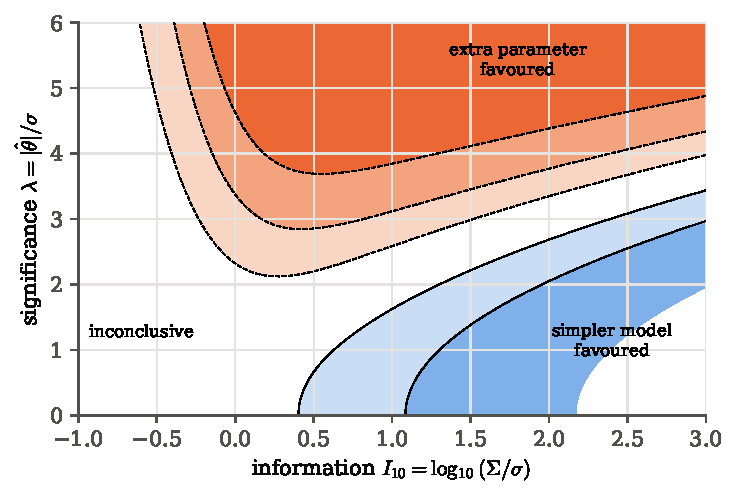
\includegraphics[width=0.72\linewidth]{figures/ch05/evidence_plane.pdf}
\caption{The Bayes factor for one extra parameter with Gaussian prior and likelihood,
over the plane of information (how much narrower the likelihood is than the prior, in
powers of ten) and significance (how many standard deviations the measurement lies
from zero). Contours are at $\lvert\ln B\rvert=1$, $2.5$, $5$. Blue: the simpler model
is favoured; orange: the extra parameter is favoured; white: inconclusive. A wider prior
moves a result to the right.}
\label{5c:fig:plane}
\end{figure}

What happens if the significance stays fixed while the data grow? With $n$
measurements of unit noise,
$\sigma=1/\sqrt n$; take $\Sigma=1$ and a result exactly at $\lambda=1.96$, the
two-sided $p=0.05$ of \cref{ch:04}. The Bayes factor \eqref{5c:eq:gauss-bf} is
$\sqrt{1+n}\,\exp[-\tfrac12(1.96)^2\,n/(1+n)]$, which grows like $\sqrt n$. With even
prior odds the posterior probability of the null (\cref{5c:fig:lindley}) is
$\FiveCLinPzeroN$ at $n=1$, $\FiveCLinPzeroNk$ at $n=10^3$ and $\FiveCLinPzeroNm$ at
$n=10^6$. At a fixed ``$1.96\sigma$'' the data favour the null once $n$ exceeds about
$\FiveCLinNhalf$, and overwhelmingly so for large samples. Even at $p=0.01$
($\lambda=2.58$) the probability of the null at $n=10^6$ is $\FiveCLinPzeroNkk$. This is
\newterm{Lindley's paradox} \cite{Lindley1957}: the same p-value means evidence \emph{against} the null in a
small experiment and evidence \emph{for} it in a large one.

\begin{figure}[htbp]
\centering
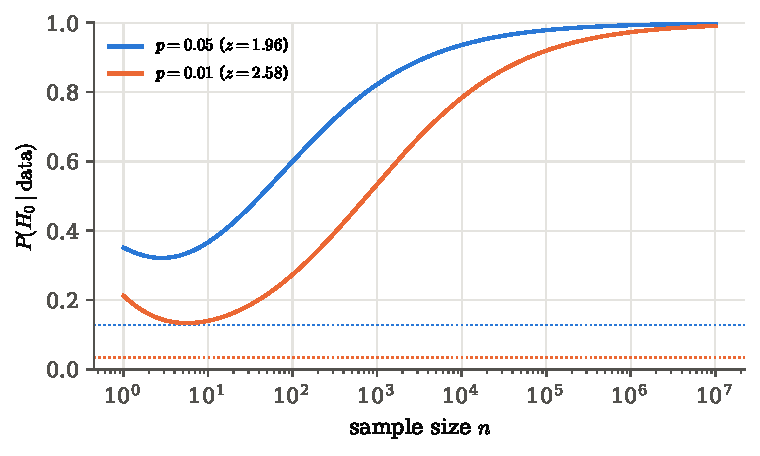
\includegraphics[width=0.75\linewidth]{figures/ch05/lindley.pdf}
\caption{Lindley's paradox. The posterior probability of ``no effect'' for a result
held at fixed significance ($1.96\sigma$, blue; $2.58\sigma$, orange) as the sample size
grows, with a unit-width prior on the effect and even prior odds. The dotted lines are
the lowest value any prior could give (the bound of \cref{5c:sec:pvalues}).}
\label{5c:fig:lindley}
\end{figure}

There is nothing paradoxical in the mechanism. At fixed significance the measured
effect $\hat\theta=1.96/\sqrt n$ shrinks as $n$ grows. The alternative spread its prior
over effects of size $\Sigma=1$, and the data increasingly say that the effect, if there
is one, is far smaller than anything $M_1$ expected. The measurement becomes a successful
prediction of $M_0$. The p-value, which only asks how surprising the data are under
$M_0$, cannot see this. Large modern data sets (Planck maps, LHC luminosities, years of
detector time) are exactly where the two answers part company, which is why ``how many
sigma'' is not by itself a good measure of the evidence for a new effect
\cite[\S5.4]{Trotta2008}.

\subsection{What a p-value can and cannot say}
\label{5c:sec:pvalues}

Wasserman's version of the Bayesian test makes the link to \cref{ch:04} explicit
\mainref{pp.~184--185}. Take the data $x^n=(x_1,\dots,x_n)$ with likelihood
$\Like(\theta)$, and test $H_0:\theta=\theta_0$ against $H_1:\theta\ne\theta_0$. Give each
hypothesis prior probability $\tfrac12$, and give $\theta$ a prior density $f(\theta)$
under $H_1$. Then
\begin{equation}
  \Prob(H_0\given x^n)
  =\frac{\Like(\theta_0)}{\Like(\theta_0)+\int\Like(\theta)f(\theta)\,\dd\theta} ,
  \label{5c:eq:aos-test}
\end{equation}
which is \eqref{5c:eq:model-post} with $Z_0=\Like(\theta_0)$ and $Z_1$ the average of the
likelihood over $f$. The prior $f$ matters here in a way it did not in estimation, and it
must be proper. Is there anything we can say whatever $f$ is? Yes: a bound. An average
cannot exceed the maximum, so $\int\Like f\,\dd\theta\le\Like(\hat\theta)$, where
$\hat\theta$ is the maximum-likelihood value. Putting this into the denominator,
\begin{equation}
  \Prob(H_0\given x^n)\;\ge\;\frac{\Like(\theta_0)}{\Like(\theta_0)+\Like(\hat\theta)} .
  \label{5c:eq:aos-bound}
\end{equation}
For a Gaussian measurement at significance $z$, $\Like(\hat\theta)/\Like(\theta_0)=e^{z^2/2}$,
which at $z=1.96$ is $\FiveCLinBoundLR$. So a result at ``$p=0.05$'' leaves the null with
posterior probability at least $\FiveCLinBound$, whatever prior the alternative is given.
The most favourable prior for $H_1$ is a spike at $\hat\theta$, chosen after seeing the
data, which is cheating; any honest prior does worse.

A less extreme and more useful bound restricts the alternative to priors that are
symmetric about $\theta_0$ and do not increase away from it. Sellke, Bayarri and Berger
showed that over this class \cite{Sellke2001}
\begin{equation}
  B_{10}\;\le\;\bar B_{10}=-\frac{1}{e\,p\ln p}\qquad(p\le e^{-1})
  \label{5c:eq:sellke}
\end{equation}
for a p-value $p$ \cite[\S4.5, eq.~(27)]{Trotta2008}. It turns a significance into the
best odds it could possibly support:

\begin{center}
\small
\renewcommand{\arraystretch}{1.15}
\begin{tabular}{@{}lcccccc@{}}
\toprule
p-value & $0.05$ & $0.01$ & $0.003$ & $0.001$ & $3\times10^{-4}$ & $5.7\times10^{-7}$\\
significance $z$ & $\FiveCSelaZ$ & $\FiveCSelbZ$ & $\FiveCSelcZ$ & $\FiveCSeldZ$ & $\FiveCSeleZ$ & $\FiveCSelfZ$\\
best odds $\bar B_{10}$ & $\FiveCSelaB$ & $\FiveCSelbB$ & $\FiveCSelcB$ & $\FiveCSeldB$ & $\FiveCSeleB$ & $\FiveCSelfB$\\
$\ln\bar B_{10}$ & $\FiveCSelalnB$ & $\FiveCSelblnB$ & $\FiveCSelclnB$ & $\FiveCSeldlnB$ & $\FiveCSelelnB$ & $\FiveCSelflnB$\\
\bottomrule
\end{tabular}
\end{center}

\noindent A ``$99\%$'' result supports odds of $8:1$ at best, short of the moderate
level. Strong evidence at best needs about $3.6\sigma$. A useful rule of thumb is to read
an $s$-sigma result as roughly an $(s-1)$-sigma one \cite[p.~18]{Trotta2008}. The
$5\sigma$ discovery convention of particle physics corresponds to best odds of about
$4.5\times10^4:1$.

\begin{keyidea}[Significance is not evidence]
A p-value is the probability, computed as if $H_0$ were true, of the observed
result \emph{together with every result lying further out in the same direction}
(\cref{4a:sec:pvalue-def}). A Bayes factor compares how probable the result actually
observed was under $H_0$ and under a specified alternative. Even with the alternative's
prior chosen as favourably as honesty allows, a $2\sigma$ result supports odds of at most
about $2.5:1$, and at fixed significance larger samples favour the null (Lindley).
\end{keyidea}

The difference lies in those further-out results. The p-value collects the probability of
outcomes that were not observed, and it never asks what the alternative predicted. The
Bayes factor uses only the observed outcome, under both hypotheses. When a paper
reports ``$3\sigma$ evidence'', the Bayes factor is the number that says how much the
data should move us, and the prior on the new effect is what the claim is really about.
\section{Nested models, shortcuts and model averaging}
\label{5c:sec:nested}

Almost every model comparison in cosmology has the shape of our bump hunt. The base
model is $\Lambda$CDM with its six parameters. The candidate extension adds a
parameter that is zero, or some other fixed value, in the base model: the spatial
curvature $\Omega_k$, the running $\dd n_s/\dd\ln k$, the tensor ratio $r$, the
non-Gaussianity $f_{\rm NL}$, the dark-energy equation of state through $w+1$, an
extra number of neutrino species $N_\nu-3.04$, and upwards of twenty more
\srcref{HobsonBMC}{Table~4.2}. In the bump hunt the base model is the line and the
extension adds a bump that disappears at $A=0$. The simpler model sits inside the
bigger one as a special value of the new parameter. Such models are called
\newterm{nested}. Nesting makes the Bayes factor easier to compute, makes it natural to
combine the models, and leads to some useful approximations.

\subsection{The Savage--Dickey density ratio}
\label{5c:sec:sddr}

Write the parameters of the bigger model $M_1$ as $(\bm\phi,\psi)$: the common
parameters $\bm\phi$ (the line, $a$ and $b$) and the new parameter $\psi$ (the
amplitude $A$). The simpler model $M_0$ is $M_1$ with $\psi$ fixed at $\psi_*$ ($A=0$).
Two conditions make the models genuinely nested \srcref{HobsonBMC}{(4.12)},
\cite[eq.~(22)]{Trotta2008}:
\begin{enumerate}[itemsep=1pt,leftmargin=1.6em]
  \item the likelihoods agree at the special value:
        $p(\data\given\bm\phi,\psi_*,M_1)=p(\data\given\bm\phi,M_0)$;
  \item the prior of $M_1$ factorises into the prior of $M_0$ for the common
        parameters times a prior for the new one:
        $p(\bm\phi,\psi\given M_1)=p(\bm\phi\given M_0)\,p(\psi\given M_1)$.
\end{enumerate}
Now ask a question about the bigger model alone: after the data, how probable is it
that the new parameter sits at its special value? That is the posterior density of
$\psi$ at $\psi_*$, and it turns out to contain the Bayes factor:
\begin{align}
  p(\psi_*\given\data,M_1)
  &\eqby{1}\int p(\bm\phi,\psi_*\given\data,M_1)\,\dd\bm\phi
   \eqby{2}\frac{1}{Z_1}\int p(\data\given\bm\phi,\psi_*,M_1)\,
      p(\bm\phi\given M_0)\,p(\psi_*\given M_1)\,\dd\bm\phi \nonumber\\
  &\eqby{3}\frac{p(\psi_*\given M_1)}{Z_1}\int p(\data\given\bm\phi,M_0)\,
      p(\bm\phi\given M_0)\,\dd\bm\phi
   \eqby{4}p(\psi_*\given M_1)\,\frac{Z_0}{Z_1} .
  \label{5c:eq:sddr-derivation}
\end{align}
\begin{explain}
  \item The marginal posterior of $\psi$: integrate the joint posterior over the common
        parameters.
  \item Bayes' theorem in $M_1$: likelihood times prior over the evidence $Z_1$, with the
        factorised prior of condition 2.
  \item Condition 1 replaces the likelihood by that of $M_0$; the prior density of
        $\psi$ at $\psi_*$ is a constant and comes out.
  \item The remaining integral is the evidence $Z_0$ of the simpler model,
        \eqref{5c:eq:evidence}.
\end{explain}
Rearranged, this is the \newterm{Savage--Dickey density ratio}
\srcref{HobsonBMC}{(4.13)}, \cite[eq.~(23)]{Trotta2008}.

\begin{workdef}[Savage--Dickey density ratio]
For nested models with a factorised prior,
\[
  B_{01}=\frac{Z_0}{Z_1}=\frac{p(\psi_*\given\data,M_1)}{p(\psi_*\given M_1)} ,
\]
\unpack{how much the data raised (or lowered) the probability density of the new
parameter at its ``absent'' value}. \emph{Operationally:} run the bigger model only,
histogram the samples of $\psi$ near $\psi_*$, and divide the height of the normalised
histogram there by the prior density.
\end{workdef}

The ratio has a direct reading. If the data pile up the posterior of the new parameter
at its null value, higher than the prior put it, the simpler model gains; if they push
the posterior away from it, the simpler model loses. Only a one-dimensional marginal
density is needed, and its normalisation is a one-dimensional integral, so there is no
high-dimensional evidence integral left to do.

\paragraph{Example: the bump amplitude at zero.}
Take the data without a bump. The new parameter is $\psi=A$ with $\psi_*=0$ and prior
density $p(A=0\given M_1)=1/A_{\max}=0.1$. The bump position $\mu$ exists only in $M_1$,
but at $A=0$ the likelihood does not depend on it and its prior integrates to one, so
the derivation goes through with $\mu$ integrated along with $\bm\phi$. On the grid,
the posterior density of $A$ at $A=0$ times $A_{\max}$ is $\FiveCSdGridZero$, which is the
exact $B_{01}=1/B_{10}=\FiveCSdExact$ of \cref{5c:sec:bump}. From a Markov chain
(\cref{5c:sec:ratios}) we estimate the density by the fraction of samples with
$A<\FiveCSdBin$, divided by $\FiveCSdBin$; this gives
$B_{01}\approx\FiveCSdChain\pm\FiveCSdChainErr$, where the error comes from splitting
the chain into twenty batches. How close this comes to the exact value varies from run
to run, for two reasons. The estimate is an average over the first bin, and the
posterior density changes across it (the grid average over the bin is
$\FiveCSdAvg$); a finer bin needs more samples. And the chain moves into and out of the
first bin slowly, so twenty batches can understate its random error.

For the data \emph{with} a bump the same estimate is much harder. There $B_{01}=1/\FiveCBumpB$,
so the posterior density at $A=0$ is small and few samples land there. A histogram is
accurate only where samples land, so the estimate is noisy. This is the known weakness
of the method: it is noisy exactly when the simpler model is disfavoured
\srcref{HobsonBMC}{p.~89}. The factorisation condition can also fail quietly, for
instance when a prior boundary of the common parameters depends on the new one.

\subsection{Model averaging}
\label{5c:sec:averaging}

Sometimes no model wins clearly, and we still want the best statement about a quantity
$\theta$ that all the models share. Probability theory gives it directly: we do not know
which model is true, so we sum the joint posterior over the models,
\begin{equation}
  p(\theta\given\data)=\sum_i p(\theta\given\data,M_i)\,\Prob(M_i\given\data),
  \label{5c:eq:bma}
\end{equation}
the posterior of $\theta$ inside each model, weighted by the probability of that model
\srcref{Kruschke}{\S10.4}, \srcref{HobsonBMC}{\S4.2}. This is \newterm{Bayesian model
averaging}. For the two coin factories of \cref{5c:sec:bf} it gave the averaged mean bias
$\FiveCFacMeanAvg$, between the two factories' $\FiveCFacMeanOne$ and
$\FiveCFacMeanTwo$, with the tail-biased factory showing up as a long left tail of the
averaged posterior.

A model in which $\theta$ is fixed still takes part. The line model fixes the amplitude
$A$ at $0$, so it contributes a spike $\Prob(M_0\given\data)\,\delta(\theta)$ to the
average. Hobson and collaborators compare the averaged posterior to a quantum
superposition that later data may collapse onto fewer models \srcref{HobsonBMC}{p.~82}.
Predictions of future data are averaged the same way. Basing them on the winning model
alone ignores the probability that it is wrong.

\paragraph{Example: which dark-energy model?}
Five models of the dark-energy equation of state $w$ were compared with the same
supernova, CMB and large-scale-structure data \srcref{HobsonBMC}{Table~4.5}. Model I is
$\Lambda$CDM, $w=-1$ exactly. Models II and III let $w$ take a constant value with
priors $-1\le w\le-0.33$ and $-2\le w\le-0.33$. Model IV gives $w$ two parameters,
$w(a)=w_0+w_a(1-a)$ with $-2\le w_0\le-0.33$ and $-1.33\le w_a\le1.33$, and model V
lets $w(a)$ vary with redshift, between $-1$ and $1$ for $0\le z\le2$. The log Bayes factors against $\Lambda$CDM are
$0$, $-1.3$, $-1.8$, $-2.0$ and $-4.1$. With equal prior probability for each model,
the posterior probabilities are $e^{\ln B_{i{\rm I}}}$ divided by their sum:
\begin{align*}
  \Prob(M_{\rm I}\given\data)
  &\eqby{1}\frac{1}{1+e^{-1.3}+e^{-1.8}+e^{-2.0}+e^{-4.1}}
   =\frac{1}{1+0.273+0.165+0.135+0.017}=0.63 ,
\end{align*}
\begin{explain}
  \item Equation \eqref{5c:eq:model-post} with equal priors: each model's share is its
        evidence over the total, and dividing every evidence by that of $\Lambda$CDM turns
        the evidences into $e^{\ln B}$.
\end{explain}
and the other four models get $0.17$, $0.10$, $0.09$ and $0.01$ in the same way. Every
extension fits at least as well as $\Lambda$CDM at its best, since each contains
$w=-1$. The evidence prefers $\Lambda$CDM because the extensions spread their priors
over values of $w$ the data exclude, and the more parameters or the wider the range,
the larger the penalty. None of the extensions is decisively ruled out
(no $\lvert\ln B\rvert$ exceeds $5$), and the probabilities depend on the prior ranges
chosen for $w$, which is the lesson of \cref{5c:sec:prior-width}.

\paragraph{Does the answer you need depend on the model?}
Averaging is the formal remedy for model uncertainty. The informal remedy is a
\newterm{sensitivity analysis}: fit several reasonable models and check whether the
quantity you actually care about changes \srcref{Lambert}{\S10.8}. Lambert's example is a
rainfall model for sizing a dam. A two-state model (dry, wet) and a three-state model
(dry, wet, persistently wet) fit $100$ days of rain equally well on every standard
test. But let each generate long rain series, and the three-state model gives far more
probability to long runs of wet days. Long wet runs are the very quantity the dam
depends on. So fit quality cannot choose between the models, and the conclusion that
matters differs between them. The cautious report gives the answer of the pessimistic
model and says why. The same habit applies
to a forecast of a background tail under different fit functions, or of a cosmological
parameter under different sets of nuisance parameters. A sensitivity analysis matters
most when data are few or the decision is sensitive to the modelling choice.

\subsection{How many bumps?}
\label{5c:sec:how-many}

Sivia's ``how many lines are there?'' is the multi-model version of the bump hunt
\srcref{Sivia}{\S4.2}. A spectrum is a sum of $M$ peaks of known shape on a background,
$M$ is unknown, and each value of $M$ is a model with $2M$ peak parameters (amplitudes
and positions). With a uniform prior on $M$ over a few values, $\Prob(M\given\data)$ is
proportional to the evidence $Z_M$ \srcref{Sivia}{(4.15)}, a $2M$-dimensional integral
over a uniform box of amplitudes and positions \srcref{Sivia}{(4.16)--(4.19)}.

We do it for $M=0,1,2$ bumps on our line, with the line integrated out exactly as in
\eqref{5c:eq:dchi2} and the priors of \cref{5c:sec:bump} for each bump. For two bumps,
$\chi^2_{\min}$ minus the line's $\chi^2_{\min}$ is a quadratic form in $(A_1,A_2)$
with coefficients $\bm r\cdot\bm u_{\mu_j}$ and $\bm u_{\mu_j}\cdot\bm u_{\mu_k}$, so the
four-dimensional grid ($81$ amplitudes and $161$ positions per bump) costs only
multiplications; refining it changes $\ln Z$ by $\FiveCHmGridErr$. The box includes both
orderings of the two positions, so the $M!$ equivalent peaks of Sivia's (4.20) are
counted automatically. Besides the one-bump data we simulate a data set with two bumps of
height $\FiveCTwoA$ at $\mu=\FiveCTwoMuOne$ and $\FiveCTwoMuTwo$
(\cref{5c:fig:how-many}).

\begin{figure}[htbp]
\centering
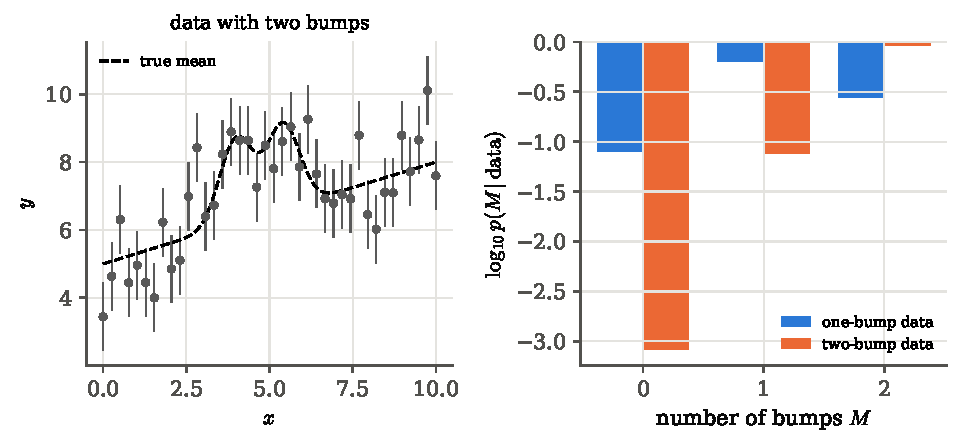
\includegraphics[width=\linewidth]{figures/ch05/how_many_bumps.pdf}
\caption{How many bumps? Left: forty points containing two overlapping bumps, with the
true mean curve. Right: the posterior probability of each number of bumps, in powers of
ten, for the one-bump data of \cref{5c:fig:bump-fits} and for the two-bump data.}
\label{5c:fig:how-many}
\end{figure}

\begin{center}
\small
\renewcommand{\arraystretch}{1.15}
\begin{tabular}{@{}l|ccccc|ccccc@{}}
\toprule
 & \multicolumn{5}{c|}{one-bump data} & \multicolumn{5}{c}{two-bump data}\\
$M$ & $\chi^2_{\min}$ & AIC & BIC & $\ln Z_M$ & $\Prob(M\given\data)$
    & $\chi^2_{\min}$ & AIC & BIC & $\ln Z_M$ & $\Prob(M\given\data)$\\\midrule
$0$ & $\FiveCHmOneChiZero$ & $\FiveCHmOneAICZero$ & $\FiveCHmOneBICZero$ & $\FiveCHmOnelnZZero$ & $\FiveCHmOnePZero$
    & $\FiveCHmTwoChiZero$ & $\FiveCHmTwoAICZero$ & $\FiveCHmTwoBICZero$ & $\FiveCHmTwolnZZero$ & $\FiveCHmTwoPZero$\\
$1$ & $\FiveCHmOneChiOne$ & $\FiveCHmOneAICOne$ & $\FiveCHmOneBICOne$ & $\FiveCHmOnelnZOne$ & $\FiveCHmOnePOne$
    & $\FiveCHmTwoChiOne$ & $\FiveCHmTwoAICOne$ & $\FiveCHmTwoBICOne$ & $\FiveCHmTwolnZOne$ & $\FiveCHmTwoPOne$\\
$2$ & $\FiveCHmOneChiTwo$ & $\FiveCHmOneAICTwo$ & $\FiveCHmOneBICTwo$ & $\FiveCHmOnelnZTwo$ & $\FiveCHmOnePTwo$
    & $\FiveCHmTwoChiTwo$ & $\FiveCHmTwoAICTwo$ & $\FiveCHmTwoBICTwo$ & $\FiveCHmTwolnZTwo$ & $\FiveCHmTwoPTwo$\\
\bottomrule
\end{tabular}
\end{center}

\noindent For the one-bump data the evidence gives one bump the probability
$\Prob(M=1\given\data)=\FiveCHmOnePOne$, although the two-bump model fits better
($\chi^2_{\min}=\FiveCHmOneChiTwo$ against $\FiveCHmOneChiOne$). For the two-bump data it
gives two bumps $\FiveCHmTwoPTwo$. The $\chi^2$ column alone would always choose the most
bumps. Two data sets could be lucky, so we repeat the count on $\FiveCHmLoopR$ fresh
data sets of each kind. The evidence picks one bump in $\FiveCHmLoopOneEvOne$ of the
one-bump sets and two bumps in $\FiveCHmLoopTwoEvTwo$ of the two-bump sets.

\subsection{Information criteria}
\label{5c:sec:ic}

The table also shows two quantities that are popular because they need no integral.
Both are built from $-2\ln\Like_{\max}$, which for Gaussian noise is $\chi^2_{\min}$ plus a
constant, plus a penalty for the number of parameters $k$ \srcref{Lambert}{\S10.5},
\cite[\S4.7]{Trotta2008}, \srcref{HobsonBMC}{(4.14)}:
\[
  \mathrm{AIC}=-2\ln\Like_{\max}+2k,\qquad
  \mathrm{BIC}=-2\ln\Like_{\max}+k\ln N ,
\]
with $N$ the number of data points; smaller is better. (The table uses $\chi^2_{\min}$ for
$-2\ln\Like_{\max}$ and counts the line's two parameters, $k=2,4,6$.)

The \newterm{Bayesian information criterion} is a crude evidence. Start from the Laplace
approximation \eqref{5c:eq:laplace-evidence} with a general prior density
\cite[eqs.~(39)--(41)]{Trotta2008}:
\begin{align}
  \ln Z
  &\relby{1}{\approx}\ln\Like_{\max}+\ln\pi(\hat\params)+\frac k2\ln2\pi-\frac12\ln\det\Fish
   \nonumber\\
  &\relby{2}{\approx}\ln\Like_{\max}+\ln\pi(\hat\params)+\frac k2\ln2\pi-\frac k2\ln N-\frac12\ln\det\Fish_1
   \nonumber\\
  &\relby{3}{\approx}\ln\Like_{\max}-\frac k2\ln N=-\tfrac12\,\mathrm{BIC} .
  \label{5c:eq:bic}
\end{align}
\begin{explain}
  \item The logarithm of \eqref{5c:eq:laplace-evidence}, with $k$ parameters.
  \item For $N$ independent data points the curvature of the log-likelihood grows in
        proportion to $N$: $\Fish=N\Fish_1$, with $\Fish_1$ the curvature per data point,
        and $\det(N\Fish_1)=N^k\det\Fish_1$.
  \item Keep only the terms that grow with $N$: $\ln\Like_{\max}$ grows like $N$,
        $\ln N$ grows slowly, and the prior, $2\pi$ and $\Fish_1$ terms stay constant.
        They are dropped.
\end{explain}
So $-\tfrac12\Delta\mathrm{BIC}$ approximates $\ln B$ for large $N$. The dropped
constant terms are exactly the ones that carry the prior. That is why BIC is attractive
(no prior to choose) and also why it is limited. It charges every parameter the same
price $\tfrac12\ln N$, as if every prior range were one data point's worth of
information wide, whether the parameter is constrained or not. In our table
$-\tfrac12\Delta\mathrm{BIC}$ gives $\FiveCHmOneBIConezero$ for one bump against none on
the one-bump data, where the exact $\ln B$ is $\FiveCHmOnelnBonezero$. Our prior ranges
for the bump are wider than BIC assumes, so BIC under-charges.

The \newterm{Akaike information criterion} comes from a different question: which model will
predict new data best, measured by a Kullback--Leibler divergence
\srcref{Lambert}{\S10.5.5}. Its penalty, $2$ per parameter, is weaker still. In the
$\FiveCHmLoopR$ fresh one-bump data sets, where the truth has one bump, AIC chooses two
bumps over one in $\FiveCHmLoopOneAicTwo$, BIC in $\FiveCHmLoopOneBicTwo$, and the
evidence in $\FiveCHmLoopOneEvTwo$.

Lambert describes the Bayesian descendants of AIC: DIC, which uses the posterior mean
and the posterior variance of the log-likelihood as the penalty; WAIC, which averages
the likelihood of each data point over the posterior; and leave-one-out cross-validation
(LOO-CV), which predicts each point from a fit to all the others
\srcref{Lambert}{\S\S10.5.6--10.5.8}. Trotta relates DIC to the Bayesian complexity, the
effective number of parameters the data actually constrain \cite[\S4.6]{Trotta2008},
\srcref{HobsonBMC}{(4.9)--(4.11)}. All of these answer ``which model predicts
best?'', not ``which model produced the data?''. Lambert prefers them to Bayes factors
because of the prior sensitivity of \cref{5c:sec:prior-width}
\srcref{Lambert}{\S10.6}; cosmologists mostly compute evidences, because their models
come with physically motivated prior ranges.

\begin{taxonomy}[Which number answers which question]
\small
\renewcommand{\arraystretch}{1.12}
\begin{tabularx}{\linewidth}{@{}>{\raggedright\arraybackslash}p{2.6cm}
                               >{\raggedright\arraybackslash}X
                               >{\raggedright\arraybackslash}p{3.6cm}@{}}
\toprule
tool & what it computes & when to trust it\\\midrule
evidence $Z$, Bayes factor & probability of the data under each model, prior included & always the target; needs the prior and an integral\\
Laplace & $\Like_{\max}\times$ posterior volume / prior volume & one Gaussian-like peak well inside the prior\\
Savage--Dickey & posterior over prior density of the new parameter at its null value & nested models, factorised prior, enough samples near the null\\
BIC & $\ln Z$ keeping only terms that grow with $N$ & many independent data, all parameters constrained, priors about one datum wide\\
AIC, DIC, WAIC, LOO-CV & expected accuracy of predictions for new data & when prediction, not the generating model, is the question\\
$\Delta\chi^2$, p-value & improvement of the best fit; surprise under the null & never on its own for comparing models\\
\bottomrule
\end{tabularx}
\end{taxonomy}

\subsection{Estimating a difference, or comparing models?}
\label{5c:sec:estimate-or-compare}

A trigger is upgraded. Before the upgrade $x_1=\FiveCEffXone$ of $n_1=\FiveCEffNone$ test
pulses fired it; after, $x_2=\FiveCEffXtwo$ of $n_2=\FiveCEffNtwo$. Did the efficiency
change? There are two different questions hidden in these words.

\paragraph{Estimation: by how much did it change?}
Give the two efficiencies $p_1,p_2$ independent flat priors. Their posteriors are
independent, $p_j\given x_j\sim\mathrm{Beta}(x_j+1,n_j-x_j+1)$, and the posterior of the
change $\tau=p_2-p_1$ is obtained by drawing pairs and subtracting, exactly as in
Wasserman's example of two binomials \mainref{pp.~183--184}. With $\FiveCEffDraws$ draws
(\cref{5c:fig:eff}), $\Prob(\tau>0\given\data)=\FiveCEffPup$, the posterior mean of $\tau$
is $\FiveCEffMean$, and the central $95\%$ interval is $[\FiveCEffLo,\FiveCEffHi]$.

\begin{figure}[htbp]
\centering
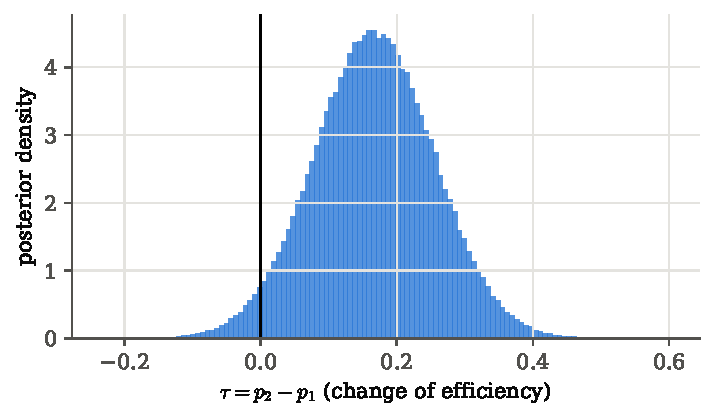
\includegraphics[width=0.7\linewidth]{figures/ch05/two_efficiencies.pdf}
\caption{The posterior of the change of trigger efficiency, from $2\times10^5$ pairs of
draws of the two Beta posteriors. About $97\%$ of the area lies to the right of zero.
The picture answers ``by how much did it change?'' and says nothing about whether the
change is exactly zero, which has zero probability under this continuous posterior.}
\label{5c:fig:eff}
\end{figure}

\paragraph{Comparison: did it change at all?}
Now let the hypotheses be two models. $M_{\rm same}$: one efficiency $p$ for both
periods, flat prior. $M_{\rm diff}$: independent $p_1,p_2$, flat priors. The evidence of
each is a Beta integral like \eqref{5c:eq:beta-evidence}; the binomial coefficients are
the same in both and cancel in the ratio:
\begin{align}
  B_{\rm same,diff}
  &\eqby{1}\frac{\int_0^1p^{x_1+x_2}(1-p)^{n_1+n_2-x_1-x_2}\,\dd p}
     {\int_0^1p_1^{x_1}(1-p_1)^{n_1-x_1}\dd p_1\int_0^1p_2^{x_2}(1-p_2)^{n_2-x_2}\dd p_2}
   \nonumber\\
  &\eqby{2}\frac{B(x_1+x_2+1,\,n_1+n_2-x_1-x_2+1)}{B(x_1+1,n_1-x_1+1)\,B(x_2+1,n_2-x_2+1)} .
  \label{5c:eq:eff-bf}
\end{align}
\begin{explain}
  \item The evidences \eqref{5c:eq:evidence} with flat priors (density one on $[0,1]$ and
        on $[0,1]^2$); the likelihood of the two samples is a product of two binomials.
  \item Each integral is a Beta function, as in \eqref{5c:eq:beta-evidence}.
\end{explain}
Numerically $B_{\rm same,diff}=\FiveCEffBsame$, so with even prior odds
$\Prob(M_{\rm same}\given\data)=\FiveCEffPsame$.

The two answers look contradictory: probability $\FiveCEffPup$ that the efficiency went
up, and probability $\FiveCEffPsame$ that it did not change. They are not, because they
answer different questions with different priors.
\begin{itemize}[itemsep=1pt,leftmargin=1.2em]
  \item The estimation put zero prior probability on ``exactly no change'', since a
        continuous prior gives any single value probability zero.
  \item The comparison put half of all prior probability on exactly that value, and
        spread the other half over all pairs $(p_1,p_2)$, most of which the data exclude.
\end{itemize}
Which is right depends on the physics. If the upgrade could plausibly have done nothing at all (a
firmware change that might not have been loaded), the point hypothesis deserves its
prior mass and the comparison is the right question. If the upgrade certainly changed
something, and we want to know how much, estimation is the right question. Kruschke
makes the same point about restricted models with negligible prior plausibility: testing
every possible equality among nine baseball positions gives $21147$ restricted models,
most of which nobody believes, and estimation of the full model is more informative
\srcref{Kruschke}{\S10.5.1}. Lambert's advice is similar: when one model extends
another, estimate within the bigger model and check its predictions
\srcref{Lambert}{\S10.7}.

\begin{pitfall}[A point null is a strong claim]
Comparing ``the effect is exactly zero'' with ``the effect is something'' gives the point
null a finite share of prior probability on a single value. That is appropriate when
theory singles the value out ($n_s=1$, $\Omega_k=0$, $w=-1$, a symmetry that forbids a
coupling). It is not appropriate for effects that are surely nonzero but possibly small;
there the question is the size of the effect, and a credible interval answers it.
\end{pitfall}
\section{Why we need sampling}
\label{5c:sec:sampling}

The denominator of Bayes' theorem, the integral over all parameter values, is the part
of Bayesian inference that does not scale to many parameters. Every evidence so far
was computed exactly or on a small grid. The coin factories had a Beta-function
formula. The bump model had four parameters, but two of them, the line, entered
linearly and could be integrated by hand, which left a two-dimensional grid. Real
problems are not so kind. The base cosmological model has six parameters. Each
evaluation of its CMB likelihood runs a Boltzmann code and takes of order a second.
Its extensions add more parameters, none of them linear \srcref{HobsonBMC}{p.~87}.
There are two ways out. For parameters, never compute the denominator. For models,
compute it with an algorithm that spends its effort where the likelihood is.

\subsection{The cost of a grid}
\label{5c:sec:grid-cost}

A grid needs about $w/\Delta$ points along each axis to cover a width $w$ with
resolution $\Delta$, so $(w/\Delta)^D$ points in $D$ dimensions
\srcref{HobsonBMC}{p.~58}, \srcref{Sivia}{\S3.4}, \srcref{Kruschke}{\S5.4}. The exponent
is the whole problem. We can watch it happen by computing the bump evidence of
\cref{5c:sec:bump} the brute-force way, on a grid over all four parameters $(a,b,A,\mu)$
with $n$ points per axis and no analytic help (\cref{5c:fig:grid-cost}). The wall time
grows as $n^4$. With $n=\FiveCGcNsmall$ the answer is $\ln B_{10}=\FiveCGcLnBsmall$,
wrong by more than a unit because the grid is too coarse to resolve the peak; with
$n=\FiveCGcNmid$ it is $\FiveCGcLnBmid$; with $n=\FiveCGcNmax$ it is $\FiveCGcLnBmax$,
against the exact $\FiveCGcExact$, after $\FiveCGcTmax$ seconds.

\begin{figure}[htbp]
\centering
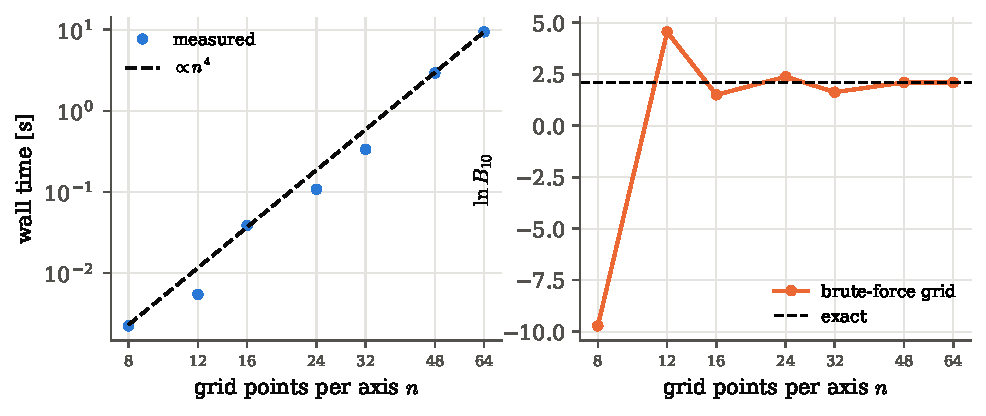
\includegraphics[width=\linewidth]{figures/ch05/grid_cost.pdf}
\caption{The bump evidence by brute force over the four-dimensional prior box. Left:
the wall time grows as the fourth power of the number of points per axis (dashed line).
Right: the log Bayes factor from the grid settles on the exact value only once the grid
is fine enough to resolve the likelihood peak, which occupies a tiny corner of the box.}
\label{5c:fig:grid-cost}
\end{figure}

At the measured cost of $\FiveCGcTpp$ seconds per grid point, a six-parameter problem
with a thousand points per axis, $10^{18}$ points, would take $\FiveCGcSixD$ years. With
a CMB likelihood at one second per call it would take $\FiveCGcSixDcmb$ years, more
than twice the age of the Universe. And almost all of that work is wasted, because
almost every grid point sits where the likelihood is negligible. How small is the
region that matters? The bulk of the posterior occupies a fraction of about $e^{-H}$
of the prior volume. Here $H$ is the information gained from the data (the
Kullback--Leibler divergence from prior to posterior), and it grows in proportion to
the number of well-measured parameters \srcref{HobsonBMC}{p.~20}.

\subsection{Sampling the prior does not rescue us}
\label{5c:sec:prior-mc}

A grid is one way to do an integral; random points are another. The evidence is an
average of the likelihood over the prior, so draw $\params_1,\dots,\params_K$ from the
prior and average: $\hat Z=\frac1K\sum_k\Like(\params_k)$ \srcref{Kruschke}{(10.7)}. The
estimate is unbiased, and its error falls like $1/\sqrt K$ whatever the dimension. The
catch is the constant in front of $1/\sqrt K$. For the simplest test case, a Gaussian
likelihood of width $s$ centred in the unit cube $[0,1]^D$ with a uniform prior, the
relative variance of one term is
\begin{align}
  \frac{\Var_\pi[\Like]}{Z^2}
  &\eqby{1}\frac{\E_\pi[\Like^2]}{Z^2}-1
   \eqby{2}\frac{\int e^{-\lvert\params-\params_0\rvert^2/s^2}\,\dd^D\params}
     {\bigl(\int e^{-\lvert\params-\params_0\rvert^2/2s^2}\,\dd^D\params\bigr)^2}-1
   \eqby{3}\frac{(s\sqrt\pi)^D}{(s\sqrt{2\pi})^{2D}}-1
   =\Bigl(\frac{1}{2\sqrt\pi\,s}\Bigr)^{D}-1 .
  \label{5c:eq:prior-mc}
\end{align}
\begin{explain}
  \item The variance is the mean square minus the square of the mean, and the mean of
        $\Like$ over the prior is $Z$.
  \item The prior density is one on the cube, so averages over the prior are integrals;
        squaring the Gaussian halves its width parameter. We neglect the parts of the
        Gaussians outside the cube, which is exact enough for $s\ll1$.
  \item Gaussian integrals: $\int e^{-u^2/s^2}\dd u=s\sqrt\pi$ and
        $\int e^{-u^2/2s^2}\dd u=s\sqrt{2\pi}$, once per dimension.
\end{explain}
The relative error of $\hat Z$ is the square root of \eqref{5c:eq:prior-mc} divided by
$\sqrt K$. For $s=0.05$ the base is $1/(2\sqrt\pi\,s)\approx5.6$: every extra dimension
multiplies the required number of draws by more than five. With $K=\FiveCDcDraws$ draws
the simulation (\cref{5c:fig:dimension}) finds a relative error of $\FiveCDcErrTwo$ for
$D=2$ and $\FiveCDcErrFive$ for $D=5$, roughly as \eqref{5c:eq:prior-mc} predicts. For $D=8$
the estimate is so lopsided that our $20$ repeated runs cannot pin down its error: most
runs fall short, and the typical run gives only $\FiveCDcMedEight$ of the true value.
By $D=10$ the typical estimate is $\FiveCDcMedTen$ of the
true value: almost no draw lands where the likelihood is, and the rare draw that does
dominates the sum. The fraction of prior draws inside the bulk of the posterior tells
the same story: $\FiveCDcFracTwo$ at $D=2$, $\FiveCDcFracFive$ at $D=5$,
$\FiveCDcFracEight$ at $D=8$. Kruschke's verdict on prior sampling is that it may need
``a ginormous number of samples'' \srcref{Kruschke}{p.~275}.

\begin{figure}[htbp]
\centering
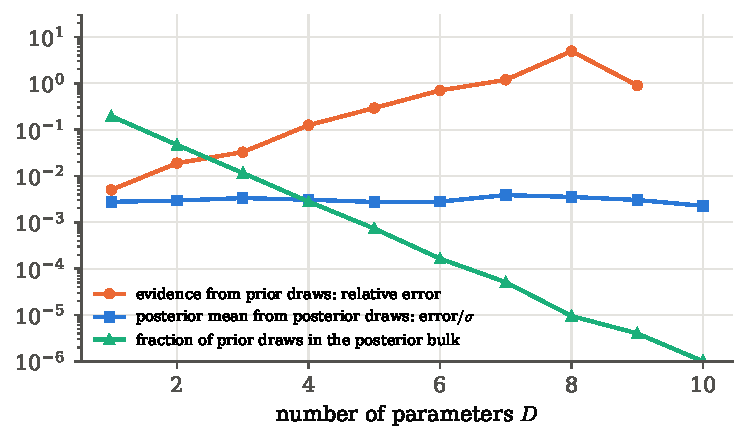
\includegraphics[width=0.8\linewidth]{figures/ch05/dimension_curse.pdf}
\caption{The curse of dimension for a Gaussian likelihood of width $0.05$ in the unit
cube, with $10^5$ draws each time. Orange: relative error of the evidence estimated
from draws of the prior, shown only while some runs still reach the likelihood peak.
Green: fraction of prior draws that land in the bulk of the
posterior. Blue: error of the posterior mean of one parameter estimated from draws of
the posterior, in units of the posterior width; it does not grow with the dimension.}
\label{5c:fig:dimension}
\end{figure}

The blue curve of \cref{5c:fig:dimension} is the hopeful one. If instead we had draws
from the \emph{posterior}, the posterior mean of a parameter would have error
$\sigma/\sqrt K$, independent of $D$: $\FiveCDcPostTwo\,\sigma$ at $D=2$ and
$\FiveCDcPostTen\,\sigma$ at $D=10$, both of the order of $1/\sqrt{10^5}\approx0.003$. This is
the central limit theorem at work on the samples \srcref{HobsonBMC}{\S3.1}, and it is why
cosmologists sample: a few thousand posterior draws summarise a posterior in any number
of dimensions \srcref{HobsonBMC}{p.~58}. What we need is a way to draw from the posterior
without knowing its normalisation.

\subsection{Ratios are all we need for parameters}
\label{5c:sec:ratios}

The normalisation of the posterior is the evidence, and it cancels from every ratio of
posterior densities:
\begin{align}
  \frac{p(\params'\given\data)}{p(\params\given\data)}
  \eqby{1}\frac{p(\data\given\params')\,p(\params')/p(\data)}{p(\data\given\params)\,p(\params)/p(\data)}
  \eqby{2}\frac{\Like(\params')\,\pi(\params')}{\Like(\params)\,\pi(\params)} .
  \label{5c:eq:ratio}
\end{align}
\begin{explain}
  \item Bayes' theorem at the two points $\params'$ and $\params$.
  \item The evidence $p(\data)$ is the same number at both points and cancels.
\end{explain}
A method that only ever asks ``how much more probable is this point than that one?''
can therefore move through parameter space using likelihood times prior alone. The
Metropolis algorithm does exactly this \cite{Metropolis1953}. From the current point
$\params$, propose a random step to $\params'$; accept it with probability
$\min(1,\text{ratio \eqref{5c:eq:ratio}})$; otherwise stay where you are and count the
current point again. We don't want the unbiased random walker, but instead a biased
random walker which spends more time in the region where probability is higher: the
accept--reject step, which uses only the ratio, is the bias. That the fraction of time
the walker spends in each region converges to the posterior probability of that region
is proved in \cref{ch:09}; here we only watch it work.

\pyfile[firstline=37,lastline=48,firstnumber=37]{code/ch05/28_sampling_evidence.py}{A
Metropolis walk on the bump posterior that uses only ratios}

Line 39 starts the walker at the best line with a small bump in the middle of the box.
Line 43 proposes a Gaussian step in all four parameters. Line 44 evaluates the logarithm
of likelihood times prior, which is $-\infty$ outside the prior box, so steps out of the
box are always rejected. Line 45 is the whole algorithm: accept if a uniform random
number is below the ratio, in logarithms. Nothing in the loop knows the evidence.

\paragraph{Example: the bump posterior from a chain.}
For the data with a bump, $\FiveCMhSteps$ steps take $\FiveCMhTime$ seconds, with
acceptance rate $\FiveCMhAcc$; we discard the first $\FiveCMhBurn$ as the walker finds
the peak. The histograms of the chain (\cref{5c:fig:mh}) lie on the grid posteriors. The
posterior mean position is $\FiveCMhMuMean$ from the chain, $\FiveCEmMuMean$ from the
standard ensemble sampler \pyname{emcee} run as a cross-check ($\FiveCEmSteps$ samples),
and $\FiveCGridMuMean$ on the grid; the mean amplitude is $\FiveCMhAMean$ (chain),
$\FiveCEmAMean$ (\pyname{emcee}) and $\FiveCGridAMean$ (grid).

\begin{figure}[htbp]
\centering
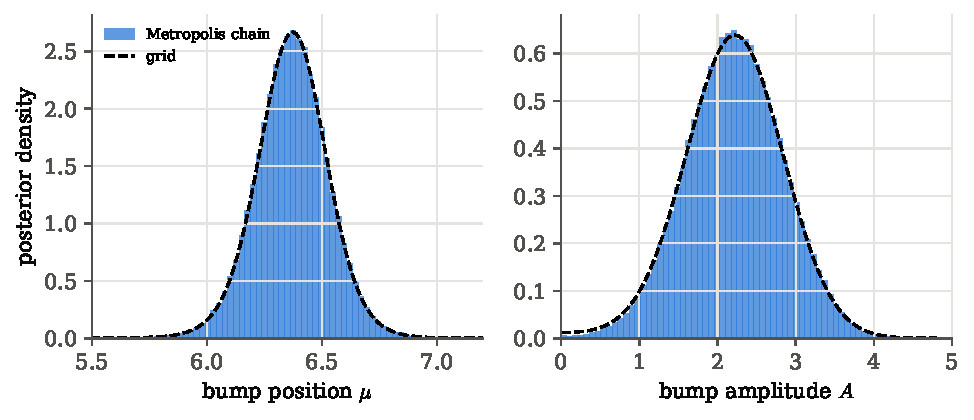
\includegraphics[width=\linewidth]{figures/ch05/mh_bump.pdf}
\caption{The posterior of the bump position and amplitude from a Metropolis chain of
$10^6$ steps that only ever evaluated ratios of likelihood times prior (histograms),
against the grid posterior (dashed). The chain never computed the evidence, yet
reproduces the normalised shape.}
\label{5c:fig:mh}
\end{figure}

A chain can miss part of a posterior, and the reason matters. Besides the peak, a bump
posterior can have a faint ``pedestal'': bumps of small amplitude anywhere in
$0<\mu<10$, which fit about as well as the line. How much probability the pedestal holds
depends on how clearly the data show the bump. For our data the grid gives it
$\FiveCMhFloorGrid$ (for $A<0.5$). The chain spends $\FiveCMhFloorChain$ of its time
there and \pyname{emcee} $\FiveCEmFloor$; $\FiveCMhNchains$ chains with different seeds
give between $\FiveCMhFloorMin$ and $\FiveCMhFloorMax$. When the pedestal holds a
noticeable share, a chain reaches it only in rare excursions, so its share is mostly
luck, set by how many times it happened to wander off the peak. Because the pedestal is
spread over the whole range of $\mu$, those rare visits matter most for the posterior
standard deviation of $\mu$: $\FiveCGridMuSd$ on the grid against $\FiveCMhMuSdMin$ to
$\FiveCMhMuSdMax$ from the chains. Why are the visits rare? A walker that takes small
local steps crosses from the peak to a distant low-amplitude region only rarely, so a
finite chain can under-represent that region. How
long a chain must run, and how to tell whether it has, is the subject of \cref{ch:09}.

\begin{inpractice}[Verification here, the instrument elsewhere]
For the bump posterior the chain can be checked against a grid, so the chain only
\emph{verifies} what we already know. In a cosmological analysis there is no grid: the
posterior of $\Lambda$CDM and its extensions from Planck, BAO and supernova data exists
only as a chain from codes such as CosmoMC \cite{LewisBridle2002}, Cobaya or
MontePython, and the chain \emph{is} the result. Convergence is then judged from the
chains themselves, for instance by comparing several chains started far apart
\cite{GelmanRubin1992}, and the samples are turned into marginal densities and triangle
plots with \pyname{getdist}. The two-step habit of this book carries over: write the
sampler from scratch once to see the mechanism, then use and cross-check the research
code.
\end{inpractice}

\subsection{The evidence needs more than a chain}
\label{5c:sec:evidence-from-samples}

A chain never computes the evidence, so it cannot simply report it. Wasserman gives a
sharp form of the difficulty \mainref{Example~11.10}. Suppose a density is known up to
its constant, $f(x)=c\,g(x)$ with $g$ known, and we can draw $n$ samples $x_1,\dots,x_n$
from $f$. Can the samples tell us $c$? Treat $c$ as a parameter. The likelihood of the
samples is $\prod_i c\,g(x_i)\propto c^n$, the same function of $c$ whatever the samples
are, so a Bayesian analysis learns nothing about $c$ from them. Yet $c$ can be
estimated another way. Estimate the density $\hat f$ from the samples at any point $x$;
then $\hat c=\hat f(x)/g(x)$.

The same trick works for the evidence. Bayes' theorem, rearranged, gives an identity
for the evidence at \emph{any} parameter value $\params$:
\begin{align}
  p(\params\given\data)=\frac{\Like(\params)\,\pi(\params)}{Z}
  \quad\Longrightarrow\quad
  Z=\frac{\Like(\params)\,\pi(\params)}{p(\params\given\data)} .
  \label{5c:eq:candidate}
\end{align}
The numerator, likelihood times prior, we can compute. The denominator is the
normalised posterior density, which the samples estimate. Here $\Like(\params)\pi(\params)$
plays the role of the known $g$, and $Z$ the role of $1/c$. The Savage--Dickey ratio of
\cref{5c:sec:sddr} is this idea for
nested models at the point $\psi=\psi_*$. The \pyname{MCEvidence} code estimates the
posterior density from the nearest-neighbour distances of chain samples
\srcref{Padilla}{\S7}. Kruschke describes a version that averages over the chain
instead of using one point \srcref{Kruschke}{(10.8)}: for any normalised density
$h(\params)$, $1/Z=\E_{\rm post}[h(\params)/(\Like(\params)\pi(\params))]$, which works
well when $h$ resembles the posterior and badly when it does not (with $h$ equal to the
prior it becomes the harmonic-mean estimator, whose variance can be infinite). All
these need a good density estimate in the region that matters, which is again hard in
many dimensions. The reliable general-purpose methods are built for the evidence from
the start.

A chain can also be made to carry the model index. Give the model label $m$ a prior and
let the sampler move in the joint space of $m$ and the parameters of each model, so that
the fraction of steps spent at $m$ estimates $\Prob(m\given\data)$, and the ratio of
the fractions estimates the posterior odds \srcref{Kruschke}{\S10.3.2}. The
difficulty is that, when the chain sits at $m=1$, the parameters that belong only to
model $2$ have no likelihood to pull them anywhere, so they wander over their whole
prior. When the chain proposes a jump to $m=2$, those parameters are almost certainly
somewhere the data exclude, and the jump is rejected. The chain rarely changes model.
The remedy is a \newterm{pseudo-prior}: while the chain sits in another model, the
idle parameters are drawn from a stand-in density placed where their own model's posterior
lives, so that a jump to that model lands somewhere sensible. A pseudo-prior costs a
preliminary run in each model, and, because it does not enter the final answer, it
only affects efficiency, not the result.

\subsection{Nested sampling}
\label{5c:sec:nested-sampling}

Skilling's nested sampling turns the $D$-dimensional evidence integral into a
one-dimensional one \cite{Skilling2006}, \srcref{HobsonBMC}{\S1.4.1}. How can that be?
The evidence only asks how much prior mass has how much likelihood; it does not care
where in parameter space that mass sits. So sort all the prior mass by likelihood. For
each likelihood level $\ell$ let
\[
  X(\ell)=\int_{\Like(\params)>\ell}\pi(\params)\,\dd\params
\]
be the prior mass enclosed by the contour $\Like=\ell$ \srcref{HobsonBMC}{(1.57)}. It
falls from $X=1$ at $\ell=0$ to $X=0$ at the maximum likelihood, and its inverse
$\Like(X)$ is the likelihood of the contour that encloses prior mass $X$
(\cref{5c:fig:ns-scheme}). Then
\begin{align}
  Z
  &\eqby{1}\int\pi(\params)\Bigl[\int_0^{\infty}\mathbb 1\bigl(\Like(\params)>\ell\bigr)\,\dd\ell\Bigr]\dd\params
   \eqby{2}\int_0^\infty\Bigl[\int_{\Like(\params)>\ell}\pi(\params)\,\dd\params\Bigr]\dd\ell
   \nonumber\\
  &\eqby{3}\int_0^\infty X(\ell)\,\dd\ell
   \eqby{4}\int_0^1\Like(X)\,\dd X .
  \label{5c:eq:ns}
\end{align}
\begin{explain}
  \item Write the positive number $\Like(\params)$ as the length of the interval
        $0<\ell<\Like(\params)$, an integral of the indicator $\mathbb1(\cdot)$, which is
        one when its condition holds and zero otherwise.
  \item Exchange the order of integration: for fixed $\ell$ the indicator restricts
        $\params$ to the region inside the contour $\Like=\ell$.
  \item The inner integral is the enclosed prior mass $X(\ell)$.
  \item The area under the decreasing curve $X(\ell)$, plotted against $\ell$, is the
        same region of the plane as the area under its inverse $\Like(X)$, plotted
        against $X$ \srcref{HobsonBMC}{(1.58)}.
\end{explain}

\begin{figure}[htbp]
\centering
\begin{tikzpicture}[font=\small]
  \begin{scope}
    \draw[softgray] (0,0) rectangle (4,4);
    \fill[formblue!8] (2,2) circle (1.748);
    \fill[formblue!16] (2,2) circle (1.354);
    \fill[formblue!28] (2,2) circle (1.049);
    \draw[form] (2,2) circle (1.748);
    \draw[form] (2,2) circle (1.354);
    \draw[form] (2,2) circle (1.049);
    \node[font=\footnotesize,formblue!80!black,fill=white,inner sep=1pt] at (3.236,3.236) {$\Like_1$};
    \node[font=\footnotesize,formblue!80!black,fill=white,inner sep=1pt] at (3.354,2) {$\Like_2$};
    \node[font=\footnotesize,formblue!80!black,fill=white,inner sep=1pt] at (2.742,1.258) {$\Like_3$};
    \fill[fibreorange] (2,2) circle (1.5pt);
    \node[anchor=north] at (2,-0.05) {parameter space (prior box)};
  \end{scope}
  \begin{scope}[xshift=5.6cm,x=5cm,y=3.6cm]
    \draw[->,softgray] (0,0) -- (1.08,0) node[right,black] {$X$};
    \draw[->,softgray] (0,0) -- (0,1.08) node[above,black] {$\Like(X)$};
    \fill[formblue!12] (0.6,0) rectangle (1,{exp(-3.6)});
    \fill[formblue!20] (0.36,0) rectangle (0.6,{exp(-2.16)});
    \fill[formblue!30] (0.216,0) rectangle (0.36,{exp(-1.296)});
    \draw[bdryred,thick,domain=0:1,samples=100] plot (\x,{exp(-6*\x)});
    \foreach \X/\lab in {0.6/X_1,0.36/X_2,0.216/X_3}{
      \draw[softgray] (\X,0) -- (\X,-0.03);
      \node[below,font=\footnotesize] at (\X,-0.03) {$\lab$};
    }
    \draw[softgray] (1,0) -- (1,-0.03) node[below,font=\footnotesize] {$1$};
    \node[bdryred,anchor=west] at (0.2,0.62) {$\Like(X)$, decreasing};
  \end{scope}
\end{tikzpicture}
\caption{Nested sampling in pictures. Left: nested likelihood contours in parameter
space; the contour $\Like_i$ encloses prior mass $X_i$, and each step moves inward. Right:
the same contours as a decreasing curve $\Like(X)$ over the unit interval of prior mass.
The evidence is the area under the curve, accumulated strip by strip (shaded), each
strip of height $\Like_i$ and width $X_{i-1}-X_i$. Here each step shrinks $X$ by the
factor $0.6$.}
\label{5c:fig:ns-scheme}
\end{figure}

A one-dimensional integral of a decreasing function is easy, if we know $\Like$ at a
sequence of known $X$ values. Nested sampling produces such a sequence with the $X$
values known statistically. Keep $N$ ``live'' points drawn from the prior. At each step:
\begin{enumerate}[itemsep=1pt,leftmargin=1.6em]
  \item find the live point with the lowest likelihood, $\Like_i$; record it and its
        estimated enclosed mass $X_i$;
  \item replace it by a new point drawn from the prior subject to $\Like>\Like_i$
        \srcref{HobsonBMC}{(1.61)};
  \item add the strip $\Like_i\,(X_{i-1}-X_i)$ to the running sum; stop when the live
        points could not add a significant amount any more.
\end{enumerate}
Why do we know $X_i$? Before step $i$ the $N$ live points are independent draws from the
prior inside the contour $\Like_{i-1}$, so their enclosed masses are uniform on
$[0,X_{i-1}]$. The discarded point is the one with the largest enclosed mass (the lowest
likelihood). The ratio $t=X_i/X_{i-1}$ is therefore the largest of $N$ uniform numbers on
$[0,1]$, whose density is $Nt^{N-1}$ \srcref{HobsonBMC}{(1.62)}: the probability that
all $N$ lie below $t$ is $t^N$, and its derivative is $Nt^{N-1}$. On average
\begin{align}
  \E[\ln t]
  &\eqby{1}\int_0^1Nt^{N-1}\ln t\,\dd t
   \eqby{2}\Bigl[t^N\ln t\Bigr]_0^1-\int_0^1t^{N}\,\frac{\dd t}{t}
   \eqby{3}-\frac1N ,
  \label{5c:eq:shrink}
\end{align}
\begin{explain}
  \item The expectation of $\ln t$ over the density $Nt^{N-1}$.
  \item Integration by parts, with $Nt^{N-1}\dd t=\dd(t^N)$.
  \item The boundary term vanishes at both ends ($t^N\ln t\to0$ as $t\to0$), and
        $\int_0^1t^{N-1}\dd t=1/N$.
\end{explain}
so $\ln X_i\approx-i/N$: each step shrinks the enclosed prior mass by about $e^{-1/N}$
\srcref{HobsonBMC}{(1.63)}. The prior mass shrinks geometrically, so the algorithm reaches
the tiny region $X\sim e^{-H}$ where the posterior lives after about $NH$ steps, a number
linear rather than exponential in the information. The uncertainty of the $X_i$ gives an
uncertainty of $\ln Z$ of about $\sqrt{H/N}$; it can also be found by redrawing the
shrinkage factors $t$ many times from $Nt^{N-1}$ and recomputing the sum
\srcref{HobsonBMC}{p.~24}.

\paragraph{Example: the bump evidence by nested sampling.}
We run nested sampling from scratch on the $(A,\mu)$ problem of \cref{5c:sec:bump}, with
the line integrated out, so that the result is the Bayes factor $B_{10}$ itself. With
$N=\FiveCNsLive$ live points the run takes $\FiveCNsIter$ steps and ends at
$\ln X=\FiveCNsLnXend$. It returns $\ln B_{10}=\FiveCNsLnZ\pm\FiveCNsErr$, the error
from redrawing the shrinkage factors, against the exact $\FiveCNsRef$
(\cref{5c:fig:ns}). The information is $H=\FiveCNsH$, so Skilling's estimate of the error
is $\sqrt{H/N}=\FiveCNsSkilling$, and $\FiveCNsRuns$ independent runs scatter with standard
deviation $\FiveCNsRunSd$ about a mean of $\FiveCNsRunMean$. The algorithm knows its own
error.

\begin{figure}[htbp]
\centering
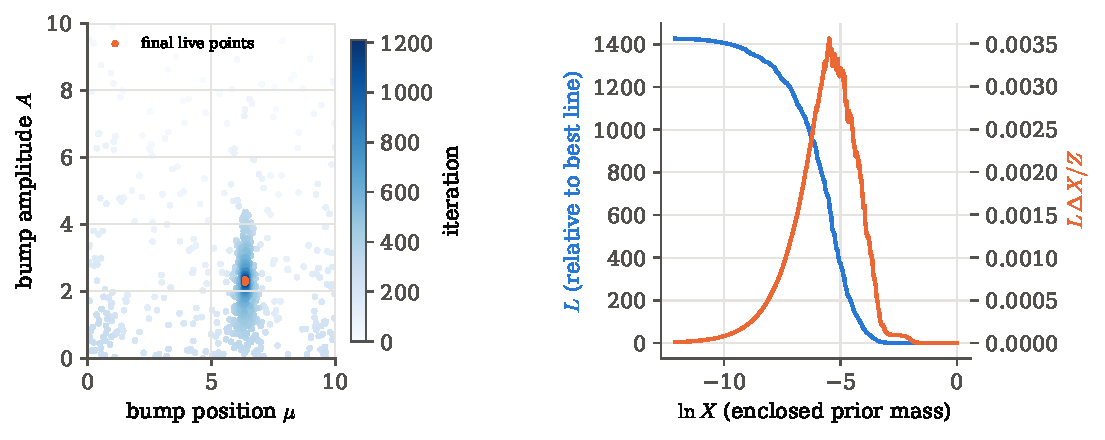
\includegraphics[width=\linewidth]{figures/ch05/nested_sampling.pdf}
\caption{Nested sampling of the bump evidence. Left: the discarded points in the plane of
bump position and amplitude, shaded by the step at which they were discarded; the early
ones are spread over the whole prior box, the late ones close in on the peak, where the
final live points sit. Right: the likelihood of the discarded points against the
logarithm of the enclosed prior mass (blue), and each point's share of the evidence
(orange). The evidence comes from a band around $\ln X\approx-5$, that is, from about
$e^{-5}$ of the prior.}
\label{5c:fig:ns}
\end{figure}

Our version is honest but naive in one place. Step 2 draws new points from the whole
prior until one beats the current lowest likelihood; late in the run almost every
draw fails, and the run spends $\FiveCNsEvalM$ million likelihood evaluations. Research
codes draw the replacement point from a short constrained Markov chain or from ellipsoids
fitted around the live points, and need of order $10^5$ likelihood evaluations for a
cosmological evidence \cite[\S4.3]{Trotta2008}. With a likelihood that takes a second,
that is the difference between a day and several years. Thermodynamic integration,
which heats a Markov chain from the prior to the posterior, is the older alternative and
typically costs about a hundred times more \cite[\S4.3]{Trotta2008},
\srcref{HobsonBMC}{\S4.4.1}. Two further options
are VEGAS, an adaptive multidimensional integrator that refines a sampling density
on the fly and is popular in particle physics, and parallel tempering, in which Markov
chains at different ``temperatures'' (likelihood raised to a power below one, so that
the landscape is flatter) run side by side and swap states, which helps chains cross
between separated peaks \srcref{HobsonBMC}{\S4.4.1}.

\subsection{The same question for lists, parameters and models}
\label{5c:sec:same-question}

Bayes' theorem has now been used on three kinds of hypotheses, and the questions never
changed. For a short list (Monty's doors, a disease, two urns) the posterior was a set
of numbers. For the values of a continuous parameter it was a density. For whole models
it was again a set of numbers, and the probability of the data under each model was
itself an average over that model's parameters. Each time we asked the two questions of
\cref{5a:sec:denominator}: which hypotheses could have produced what we observed, and
how probable the observation was under each. For model comparison the first question
lists the models, each with its prior; the second is answered by the evidence.

The difference between the two uses lies in the evidence. For parameter estimation
inside a model the evidence cancels, and a sampler that uses only ratios delivers the
posterior. For model comparison it does not cancel, so it must be computed: exactly, by
a Laplace or Savage--Dickey approximation, or by nested sampling. The Markov chains of
\cref{ch:09} and the Fisher forecasts of \cref{ch:10} are the two tools the rest of the
book uses to answer the second question in many dimensions.

\begin{recap}
\begin{itemize}[itemsep=2pt,leftmargin=1.2em]
  \item A model is a likelihood and a prior. Its evidence $Z=\int\Like\,\pi\,\dd\params$ is
        the probability it gave to the observed data: the likelihood averaged over its
        prior.
  \item $\Prob(M_i\given\data)\propto Z_i\Prob(M_i)$; posterior odds $=$ Bayes factor
        $\times$ prior odds. The comparison says nothing about parameters; model averaging
        combines the parameter posteriors with the model probabilities as weights.
  \item No model is rejected on its own: $p(\data\given\text{not }M)$ is undefined without
        specific alternatives.
  \item Occam's razor is derived, not assumed: $Z\approx\Like_{\max}\times V_{\rm post}/V_{\rm prior}$.
        Better fits are rewarded, wasted prior range is penalised, unconstrained parameters
        cost nothing. For the bump: a best-fit gain of $e^{\FiveCBumplnLR}$ became odds of $\FiveCBumpB:1$.
  \item Read Bayes factors on the logarithmic Jeffreys scale ($\lvert\ln B\rvert=1$, $2.5$,
        $5$), as posterior odds, and with their numerical and prior uncertainty.
  \item The evidence depends on prior widths ($-\ln10$ per decade of range) and can reverse
        between two vague priors that give the same posterior; improper priors are
        forbidden. Equally informed priors, physically motivated ranges and sensitivity
        plots are the remedies.
  \item Lindley: at fixed significance, large samples favour the null. A $p$-value bounds the
        odds: at most $1/(e\,p\ln p)$ against the null, $2.5:1$ at $2\sigma$, $150:1$ at
        $3.6\sigma$.
  \item Nested models: Savage--Dickey $B_{01}=p(\psi_*\given\data)/\pi(\psi_*)$ from the bigger
        model alone; BIC is the Laplace evidence without its prior terms; AIC, WAIC and LOO
        rank predictions, a different question.
  \item Estimating a difference and testing whether it is exactly zero are different
        questions with different priors, and can give opposite-looking answers.
  \item Grids cost $n^D$ and prior sampling fails exponentially in $D$; posterior samples
        give errors independent of $D$. Ratios of posteriors do not need the evidence
        (Metropolis, \cref{ch:09}); the evidence needs its own algorithm, such as nested
        sampling, $Z=\int_0^1\Like(X)\,\dd X$ with $\ln X_i\approx-i/N$.
\end{itemize}
\end{recap}

\subsection*{Reading the literature}
\label{5c:sec:reading-list}

\begin{itemize}[itemsep=2pt,leftmargin=1.2em]
  \item \textbf{The main line.} Wasserman, \emph{All of Statistics}, Chapter~11: the
        Bayesian method, conjugate examples, simulation from the posterior, flat and
        Jeffreys priors, Bayesian testing and its prior-free bound, and the strengths and
        weaknesses of Bayesian inference \mainref{pp.~175--189}.
  \item \textbf{The gentlest route.} Kruschke, \emph{Doing Bayesian Data Analysis},
        Chapters~2 and 5 (credibility, Bayes' rule), 6 (the Beta--Bernoulli model), 10 (model
        comparison, Occam's razor, prior sensitivity) and 12 (HDIs, estimation against
        testing).
  \item \textbf{The physicist's tutorial.} Sivia, \emph{Data Analysis: A Bayesian
        Tutorial}, Chapters~1--3 (plausible reasoning, parameter estimation, the Gaussian
        approximation, marginalisation), 4 (Mr A and Mr B, how many lines) and 5
        (assigning priors).
  \item \textbf{Priors, prediction and checks.} Lambert, \emph{A Student's Guide to
        Bayesian Statistics}, Chapters~3--7 and 9 (Bayes' rule, likelihood, priors, the
        denominator, conjugacy) and 10 (predictive checks, AIC to LOO-CV, Bayes factors,
        sensitivity analysis).
  \item \textbf{Cosmology.} Hobson, Jaffe, Liddle, Mukherjee and Parkinson (eds.),
        \emph{Bayesian Methods in Cosmology}, Chapter~1 (foundations, priors, nested sampling),
        Chapter~3 (Monte Carlo parameter estimation) and Chapter~4 (model selection,
        Savage--Dickey, the Jeffreys scale, the spectral index). Trotta's review ``Bayes in
        the sky'' \cite{Trotta2008} covers evidence, Occam's razor, the Lindley paradox and
        the $p$-value calibration in cosmological language. Padilla et al.\ \cite{Padilla2019}
        is a hands-on introduction with code.
  \item \textbf{Original papers.} Kass and Raftery on Bayes factors \cite{KassRaftery1995};
        Lindley's paradox \cite{Lindley1957}; Sellke, Bayarri and Berger on calibrating
        $p$-values \cite{Sellke2001}; Skilling on nested sampling \cite{Skilling2006};
        Metropolis et al.\ on the algorithm of \cref{ch:09} \cite{Metropolis1953}.
  \item \textbf{Pictures.} \emph{Seeing Theory}, chapter ``Bayesian Inference'', for
        interactive versions of the updating examples.
\end{itemize}

\clearpage
\raggedbottom
\section*{Chapter summary}
\addcontentsline{toc}{section}{Chapter summary}
\label{5c:sec:summary}

Bayesian inference turns the direction of probability around. Instead of asking what a
hypothesis predicts, we start from an outcome already observed and ask which hypotheses
might lie behind it, and how probable each is after the fact. Bayes' theorem answered
this question first for a short list of hypotheses, then for a continuous parameter,
and then for whole models, where the denominator we had been ignoring became the
quantity of interest. In the pipeline of the book,
\[
  \text{model}\to\text{data}\to\text{summary }S\to P(S\given\theta)\to\boxed{\text{infer physics}},
\]
Bayesian inference is the last arrow: the sampling distribution $P(S\given\theta)$ becomes
the likelihood, and the posterior over parameters and models is the inference.
\Cref{ch:04} gave the frequentist form of the same arrow.

\begin{center}
\small
\renewcommand{\arraystretch}{1.15}
\begin{tabularx}{\linewidth}{@{}>{\raggedright\arraybackslash}p{3.3cm}
                               >{\raggedright\arraybackslash}X
                               >{\raggedright\arraybackslash}p{2.7cm}@{}}
\toprule
\multicolumn{3}{@{}l}{\textbf{Bayes' theorem with a list of hypotheses}}\\
concept & operational meaning & used later in\\\midrule
prediction vs inference & $\Prob(E\given H)$ reads the tree forward; $\Prob(H\given E)$ asks which path produced the observed leaf & every chapter\\
joint table, logical not causal & one table of (hypothesis, outcome) probabilities: columns predict, rows infer; a posterior links hypothesis and evidence logically, it does not say the evidence caused anything & every chapter\\
Bayes' theorem & product rule in both orders: $\Prob(H\given E)=\Prob(E\given H)\Prob(H)/\Prob(E)$ & \cref{ch:08,ch:09}\\
information shrinks the sample space & conditioning on $E$ keeps only the region where $E$ holds and re-measures everything inside it & \cref{ch:08}\\
unit-square picture & priors are widths, likelihoods heights, posterior = surviving rectangle over total surviving area & \cref{ch:08}\\
reasoning in words & the event; what could have produced it; its probability under each hypothesis; then priors and normalise. Monty Hall: ``Monty opened C''; what made him open that door?; $\frac12,1,0$ for car behind A, B, C; posterior $\frac13,\frac23,0$ & every chapter\\
base rates & a tall bar in a thin strip can lose to a short bar in a wide one (rare signals, trigger purity) & \cref{ch:08,ch:12}\\
reallocation of credibility & zero likelihood eliminates, zero prior can never be revived, noisy data only nudge & \cref{ch:09}\\
odds, likelihood ratio & posterior odds $=$ likelihood ratio $\times$ prior odds; independent evidence adds in logarithms & \cref{ch:08,ch:10}\\
sequential updating & yesterday's posterior is today's prior, if the data are independent given the hypothesis & \cref{ch:09}\\
denominator, prior predictive & $\Prob(E)=\sum_i\Prob(E\given H_i)\Prob(H_i)$: normaliser and forecast; needs every hypothesis & \cref{ch:06,ch:09}\\
\bottomrule
\end{tabularx}
\end{center}

\begin{center}
\small
\renewcommand{\arraystretch}{1.15}
\begin{tabularx}{\linewidth}{@{}>{\raggedright\arraybackslash}p{3.3cm}
                               >{\raggedright\arraybackslash}X
                               >{\raggedright\arraybackslash}p{2.7cm}@{}}
\toprule
\multicolumn{3}{@{}l}{\textbf{Parameter estimation}}\\
concept & operational meaning & used later in\\\midrule
posterior density & likelihood $\times$ prior on a grid, normalised; the parameter value is the hypothesis, the data the event & \cref{ch:08,ch:09}\\
conjugate priors & Beta--Binomial, Gamma--Poisson, Normal--Normal: posterior in closed form, pseudo-counts and inverse-variance weights & \cref{ch:07,ch:08}\\
posterior summaries & mean, median, mode from three losses; equal-tailed interval; HDI, the shortest set & \cref{ch:09,ch:10}\\
credible vs confidence & probability of $\theta$ in a set given the data, against coverage over repetitions & \cref{ch:08,ch:10}\\
Gaussian (Laplace) approximation & peak and curvature: $\sigma^2=(-\partial^2\ln p)^{-1}$, covariance $=-H^{-1}$, $\Delta\chi^2$ regions & \cref{ch:10}\\
marginalising, profiling & integrate nuisance parameters out (volume included) or maximise over them & \cref{ch:08,ch:09,ch:10}\\
choosing a prior & knowledge, flat (in which variable?), Jeffreys $\propto\sqrt{I}$; improper priors as limits & \cref{ch:09}\\
forgetting the prior & the likelihood dominates for many data (Bernstein--von Mises); not the same as a chain forgetting its start & \cref{ch:09}\\
posterior sampling & a histogram of draws is the density; functions of parameters for free & \cref{ch:06,ch:09,ch:12}\\
\bottomrule
\end{tabularx}
\end{center}

\begin{center}
\small
\renewcommand{\arraystretch}{1.15}
\begin{tabularx}{\linewidth}{@{}>{\raggedright\arraybackslash}p{3.3cm}
                               >{\raggedright\arraybackslash}X
                               >{\raggedright\arraybackslash}p{2.7cm}@{}}
\toprule
\multicolumn{3}{@{}l}{\textbf{Model comparison and the need for sampling}}\\
concept & operational meaning & used later in\\\midrule
evidence $Z$ & likelihood averaged over the model's prior; the probability the model gave to the data & \cref{ch:09,ch:12}\\
Bayes factor, posterior odds & $B_{12}=Z_1/Z_2$ multiplies the prior odds; quote $\ln B$ and which model is on top & \cref{ch:09,ch:12}\\
Occam factor & $Z\approx\Like_{\max}V_{\rm post}/V_{\rm prior}$; wasted prior range is penalised, unconstrained parameters are free & \cref{ch:10}\\
Jeffreys scale & $\lvert\ln B\rvert=1,2.5,5$: odds $3,12,150$; apply to posterior odds, with the prior uncertainty & \cref{ch:12}\\
prior sensitivity & $\ln B$ falls by $\ln10$ per decade of prior range; vague priors can reverse it; improper priors forbidden & \cref{ch:12}\\
Lindley, $p$-value bounds & fixed significance favours the null at large $n$; $B_{10}\le-1/(e\,p\ln p)$ & \cref{ch:08,ch:12}\\
Savage--Dickey & $B_{01}=p(\psi_*\given\data)/\pi(\psi_*)$ from the bigger model's samples & \cref{ch:09}\\
model averaging & parameter posteriors weighted by model probabilities & \cref{ch:14}\\
BIC, AIC, WAIC, LOO & crude evidence without prior terms; predictive accuracy, a different question & \cref{ch:12}\\
estimation vs comparison & ``how large is the effect?'' against ``is it exactly zero?'': different priors, different answers & \cref{ch:08,ch:12}\\
curse of dimension & grids cost $n^D$; prior draws miss the posterior; posterior draws do not care about $D$ & \cref{ch:06,ch:09}\\
ratios, Metropolis & the evidence cancels in posterior ratios; a biased random walk samples the posterior & \cref{ch:09}\\
nested sampling & $Z=\int_0^1\Like(X)\dd X$, prior mass shrinking by $e^{-1/N}$ per step, error $\sqrt{H/N}$ & \cref{ch:09,ch:12}\\
\bottomrule
\end{tabularx}
\end{center}
\clearpage
\flushbottom
  